\documentclass{emulateapj}


\slugcomment{A living LSST document (arXiv:0805.2366); version 3.0.1 of June 29, 2014}


\newcommand\x         {\hbox{$\times$}}
\newcommand\othername {\hbox{$\dots$}}
\def\eq#1{\begin{equation} #1 \end{equation}}
\def\eqarray#1{\begin{eqnarray} #1 \end{eqnarray}}
\def\eqarraylet#1{\begin{mathletters}\begin{eqnarray} #1 
                  \end{eqnarray}\end{mathletters}}
\def\mic              {\hbox{$\mu{\rm m}$}}
\def\about            {\hbox{$\sim$}}
\def\Mo               {\hbox{$M_{\odot}$}}
\def\Lo               {\hbox{$L_{\odot}$}}
\def\comm#1           {{\tt (COMMENT: #1)}}
\def\kms   {\hbox{km s$^{-1}$}}

\usepackage{graphicx}
\usepackage{xspace}

\usepackage[usenames]{color} 
%\newcommand{\B}[1]{{\color{blue} #1}}
%\newcommand{\R}[1]{{\color{red} #1}}
\newcommand{\G}[1]{{\color{red} #1}}
\newcommand{\B}[1]{{#1}}
\newcommand{\R}[1]{{\color{red}}}

\begin{document}
\title{LSST: from Science Drivers to Reference Design and Anticipated Data Products} 

%% DO NOT EDIT THIS FILE. IT IS GENERATED FROM db2authors.py"
%% Regenerate using:
%%    python support/db2authors.py > authors.tex


\author[0000-0001-5250-2633]{\v{Z}eljko~Ivezi\'{c}}
\affiliation{University of Washington, Dept.\ of Astronomy, Box 351580, Seattle, WA 98195}

\author{Steven~M.~Kahn}
\affiliation{LSST Project Office, 950 N.\ Cherry Avenue, Tucson, AZ  85719}
\affiliation{Kavli Institute for Particle Astrophysics and Cosmology, SLAC National Accelerator Laboratory, Stanford University, Stanford, CA 94025}

\author[0000-0002-9242-8797]{J.~Anthony~Tyson}
\affiliation{Physics Department, University of California, One Shields Avenue, Davis, CA 95616}

\author{Bob~Abel}
\affiliation{Olympic College, 1600 Chester Ave., Bremerton, WA 98337-1699}

\author{Emily~Acosta}
\affiliation{LSST Project Office, 950 N.\ Cherry Avenue, Tucson, AZ  85719}

\author{Robyn~Allsman}
\affiliation{LSST Project Office, 950 N.\ Cherry Avenue, Tucson, AZ  85719}

\author{David~Alonso}
\affiliation{Department of Physics, University of Oxford, Denys Wilkinson Building, Keble Road, Oxford, OX1 3RH, UK}

\author{Yusra~AlSayyad}
\affiliation{Department of Astrophysical Sciences, Princeton University, Princeton, NJ 08544}

\author{Scott~F.~Anderson}
\affiliation{University of Washington, Dept.\ of Astronomy, Box 351580, Seattle, WA 98195}

\author{John~Andrew}
\affiliation{LSST Project Office, 950 N.\ Cherry Avenue, Tucson, AZ  85719}

\author{James~Roger~P.~Angel}
\affiliation{Steward Observatory, The University of Arizona, 933 N Cherry Ave., Tucson, AZ 85721}

\author{George~Z.~Angeli}
\affiliation{Giant Magellan Telescope Organization (GMTO), 465 N.\ Halstead Street, Suite 250, Pasadena, CA 91107}

\author{Reza~Ansari}
\affiliation{Laboratoire de l'Acc\'{e}l\'{e}rateur Lin\'{e}aire, CNRS/IN2P3, Universit\'{e} de Paris-Sud, B.P.\ 34, 91898 Orsay Cedex, France}

\author{Pierre~Antilogus}
\affiliation{Laboratoire de Physique Nucl\'{e}aire et des Hautes Energies, Universit\'{e} Pierre et Marie Curie, Universit\'{e} Paris Diderot, CNRS/IN2P3, 4 place Jussieu, 75005 Paris, France}

\author{Constanza~Araujo}
\affiliation{LSST Project Office, 950 N.\ Cherry Avenue, Tucson, AZ  85719}

\author{Robert~Armstrong}
\affiliation{Department of Astrophysical Sciences, Princeton University, Princeton, NJ 08544}

\author[0000-0002-6826-8340]{Kirk~T.~Arndt}
\affiliation{Department of Physics, University of Oxford, Denys Wilkinson Building, Keble Road, Oxford, OX1 3RH, UK}

\author{Pierre~Astier}
\affiliation{Laboratoire de Physique Nucl\'{e}aire et des Hautes Energies, Universit\'{e} Pierre et Marie Curie, Universit\'{e} Paris Diderot, CNRS/IN2P3, 4 place Jussieu, 75005 Paris, France}

\author{\'{E}ric~Aubourg}
\affiliation{AstroParticule et Cosmologie, Universit\'{e} Paris Diderot, CNRS/IN2P3, CEA/lrfu, Observatoire de Paris, Sorbonne Paris Cit\'{e}, 10, rue Alice Domon et L\'{e}onie Duquet, Paris Cedex 13, France}

\author{Nicole~Auza}
\affiliation{LSST Project Office, 950 N.\ Cherry Avenue, Tucson, AZ  85719}

\author[0000-0002-5722-7199]{Tim~S.~Axelrod}
\affiliation{Steward Observatory, The University of Arizona, 933 N Cherry Ave., Tucson, AZ 85721}

\author{Deborah~J.~Bard}
\affiliation{SLAC National Accelerator Laboratory,  2575 Sand Hill Rd, Menlo Park CA 94025}

\author{Jeff~D.~Barr}
\affiliation{LSST Project Office, 950 N.\ Cherry Avenue, Tucson, AZ  85719}

\author{Aurelian~Barrau}
\affiliation{Laboratoire de Physique Subatomique et de Cosmologie, Universit\'{e} Grenoble-Alpes, CNRS/IN2P3, 53 av.\ des Martyrs, 38026 Grenoble cedex, France}

\author{James~G.~Bartlett}
\affiliation{AstroParticule et Cosmologie, Universit\'{e} Paris Diderot, CNRS/IN2P3, CEA/lrfu, Observatoire de Paris, Sorbonne Paris Cit\'{e}, 10, rue Alice Domon et L\'{e}onie Duquet, Paris Cedex 13, France}

\author{Amanda~E.~Bauer}
\affiliation{LSST Project Office, 950 N.\ Cherry Avenue, Tucson, AZ  85719}

\author{Brian~J.~Bauman}
\affiliation{Lawrence Livermore National Laboratory, 7000 East Avenue, Livermore, CA 94550}

\author{Sylvain~Baumont}
\affiliation{Sorbonne Universit\'{e}s, UPMC Univ Paris 06, UMR 7585, LPNHE, F-75005, Paris, France}
\affiliation{Laboratoire de Physique Nucl\'{e}aire et des Hautes Energies, Universit\'{e} Pierre et Marie Curie, Universit\'{e} Paris Diderot, CNRS/IN2P3, 4 place Jussieu, 75005 Paris, France}

\author[0000-0001-6661-3043]{Andrew~C.~Becker}
\affiliation{University of Washington, Dept.\ of Astronomy, Box 351580, Seattle, WA 98195}

\author{Jacek~Becla}
\affiliation{SLAC National Accelerator Laboratory,  2575 Sand Hill Rd, Menlo Park CA 94025}

\author{Cristina~Beldica}
\affiliation{NCSA, University of Illinois at Urbana-Champaign, 1205 W.\ Clark St., Urbana, IL 61801}

\author{Steve~Bellavia}
\affiliation{Brookhaven National Laboratory, Upton, NY 11973}

\author[0000-0003-1953-8727]{Federica~B.~Bianco}
\affiliation{Center for Urban Science \& Progress, New York University, Brooklyn, NY 11021}
\affiliation{Center for Cosmology \& Particle Physics, New York University, New York, 10012}

\author{Rahul~Biswas}
\affiliation{Oskar Klein Centre, Department of Physics, Stockholm University, SE 106 91 Stockholm, Sweden}

\author{Guillaume~Blanc}
\affiliation{Laboratoire de l'Acc\'{e}l\'{e}rateur Lin\'{e}aire, CNRS/IN2P3, Universit\'{e} de Paris-Sud, B.P.\ 34, 91898 Orsay Cedex, France}
\affiliation{Universit\'{e} Paris Diderot, Sorbonne Paris Cit\'{e}, F-75013 Paris, France}

\author{Jonathan~Blazek}
\affiliation{Center for Cosmology and Astro-Particle Physics, The Ohio State University, Columbus, OH 43210, USA}
\affiliation{Institute of Physics, Laboratory of Astrophysics, \'{E}cole Polytechnique Fed\`{e}rale de Lausanne (EPFL), Observatoire de Sauverny, 1290 Versoix, Switzerland}

\author{Roger~D.~Blandford}
\affiliation{Kavli Institute for Particle Astrophysics and Cosmology, SLAC National Accelerator Laboratory, Stanford University, Stanford, CA 94025}

\author{Josh~S.~Bloom}
\affiliation{Astronomy Department,  University of California, 601 Campbell Hall, Berkeley, CA 94720}

\author{Joanne~Bogart}
\affiliation{Kavli Institute for Particle Astrophysics and Cosmology, SLAC National Accelerator Laboratory, Stanford University, Stanford, CA 94025}

\author{Anders~W.~Borgland}
\affiliation{SLAC National Accelerator Laboratory,  2575 Sand Hill Rd, Menlo Park CA 94025}

\author{Kirk~Borne}
\affiliation{School of Physics, Astronomy and Computational Sciences, George Mason University, 4400 University Drive, Fairfax, VA  22030}

\author[0000-0003-2759-5764]{James~F.~Bosch}
\affiliation{Department of Astrophysical Sciences, Princeton University, Princeton, NJ 08544}

\author[0000-0003-4887-2150]{Dominique~Boutigny}
\affiliation{Universit\'{e} Grenoble-Alpes, Universit\'{e} Savoie Mont Blanc, CNRS/IN2P3 Laboratoire d'Annecy-le-Vieux de Physique des Particules, 9 Chemin de Bellevue -- BP 110, 74940 Annecy-le-Vieux Cedex, France}

\author{Craig~A.~Brackett}
\affiliation{SLAC National Accelerator Laboratory,  2575 Sand Hill Rd, Menlo Park CA 94025}

\author{Andrew~Bradshaw}
\affiliation{Physics Department, University of California, One Shields Avenue, Davis, CA 95616}

\author{William~Nielsen~Brandt}
\affiliation{Department of Astronomy and Astrophysics, The Pennsylvania State University, 525 Davey Lab, University Park, PA 16802}

\author{Michael~E.~Brown}
\affiliation{Division of Geological and Planetary Sciences, California Institute of Technology, Pasadena, CA 91125}

\author{James~S.~Bullock}
\affiliation{Center for Cosmology, University of California, Irvine, CA 92697}

\author{Patricia~Burchat}
\affiliation{Kavli Institute for Particle Astrophysics and Cosmology, SLAC National Accelerator Laboratory, Stanford University, Stanford, CA 94025}

\author{David~L.~Burke}
\affiliation{Kavli Institute for Particle Astrophysics and Cosmology, SLAC National Accelerator Laboratory, Stanford University, Stanford, CA 94025}

\author{Gianpietro~Cagnoli}
\affiliation{Laboratoire des Materiaux Avances (LMA), CNRS/IN2P3, Universit\'{e} de Lyon, F-69622 Villeurbanne, Lyon, France}

\author{Daniel~Calabrese}
\affiliation{LSST Project Office, 950 N.\ Cherry Avenue, Tucson, AZ  85719}

\author{Shawn~Callahan}
\affiliation{LSST Project Office, 950 N.\ Cherry Avenue, Tucson, AZ  85719}

\author{Alice~L.~Callen}
\affiliation{SLAC National Accelerator Laboratory,  2575 Sand Hill Rd, Menlo Park CA 94025}

\author{Srinivasan~Chandrasekharan}
\affiliation{Department of Computer Science, The University of Arizona, 1040 E 4th St, Tucson, AZ 85719}

\author{Glenaver~Charles-Emerson}
\affiliation{LSST Project Office, 950 N.\ Cherry Avenue, Tucson, AZ  85719}

\author{Steve~Chesley}
\affiliation{Jet Propulsion Laboratory, California Institute of Technology, Pasadena, CA 91109}

\author{Elliott~C.~Cheu}
\affiliation{Department of Physics, University of Arizona, 1118 E.\ Fourth Street, Tucson, AZ 85721}

\author[0000-0002-1181-1621]{Hsin-Fang~Chiang}
\affiliation{NCSA, University of Illinois at Urbana-Champaign, 1205 W.\ Clark St., Urbana, IL 61801}

\author{James~Chiang}
\affiliation{Kavli Institute for Particle Astrophysics and Cosmology, SLAC National Accelerator Laboratory, Stanford University, Stanford, CA 94025}

\author{Carol~Chirino}
\affiliation{LSST Project Office, 950 N.\ Cherry Avenue, Tucson, AZ  85719}

\author{Derek~Chow}
\affiliation{SLAC National Accelerator Laboratory,  2575 Sand Hill Rd, Menlo Park CA 94025}

\author{David~R.~Ciardi}
\affiliation{IPAC, California Institute of Technology, MS 100-22, Pasadena, CA 91125}

\author{Charles~F.~Claver}
\affiliation{LSST Project Office, 950 N.\ Cherry Avenue, Tucson, AZ  85719}

\author[0000-0001-9022-4232]{Johann~Cohen-Tanugi}
\affiliation{Laboratoire Univers et Particules de Montpellier (LUPM), Universit\'{e} de Montpellier, CNRS/IN2P3, Place Eug\`{e}ne Bataillon, 34095 Montpellier, France}

\author{Joseph~J.~Cockrum}
\affiliation{LSST Project Office, 950 N.\ Cherry Avenue, Tucson, AZ  85719}

\author[0000-0002-4774-9364]{Rebecca~Coles}
\affiliation{Center for Cosmology and Astro-Particle Physics, The Ohio State University, Columbus, OH 43210, USA}

\author[0000-0001-5576-8189]{Andrew~J.~Connolly}
\affiliation{University of Washington, Dept.\ of Astronomy, Box 351580, Seattle, WA 98195}

\author{Kem~H.~Cook}
\affiliation{Cook Astronomical Consulting, 220 Duxbury CT, San Ramon, CA 94583, USA}

\author{Asantha~Cooray}
\affiliation{Center for Cosmology, University of California, Irvine, CA 92697}

\author{Kevin~R.~Covey}
\affiliation{Western Washington University, 516 High Street, Bellingham, WA 98225}

\author{Chris~Cribbs}
\affiliation{NCSA, University of Illinois at Urbana-Champaign, 1205 W.\ Clark St., Urbana, IL 61801}

\author{Wei~Cui}
\affiliation{Department of Physics and Astronomy, Purdue University, 525 Northwestern Ave., West Lafayette, IN  47907}

\author{Roc~Cutri}
\affiliation{IPAC, California Institute of Technology, MS 100-22, Pasadena, CA 91125}

\author{Philip~N.~Daly}
\affiliation{University of Arizona, Tucson, AZ 85721}

\author{Scott~F.~Daniel}
\affiliation{University of Washington, Dept.\ of Astronomy, Box 351580, Seattle, WA 98195}

\author{Felipe~Daruich}
\affiliation{LSST Project Office, 950 N.\ Cherry Avenue, Tucson, AZ  85719}

\author{Guillaume~Daubard}
\affiliation{Laboratoire de Physique Nucl\'{e}aire et des Hautes Energies, Universit\'{e} Pierre et Marie Curie, Universit\'{e} Paris Diderot, CNRS/IN2P3, 4 place Jussieu, 75005 Paris, France}

\author{Greg~Daues}
\affiliation{NCSA, University of Illinois at Urbana-Champaign, 1205 W.\ Clark St., Urbana, IL 61801}

\author{William~Dawson}
\affiliation{Lawrence Livermore National Laboratory, 7000 East Avenue, Livermore, CA 94550}

\author{Francisco~Delgado}
\affiliation{LSST Project Office, 950 N.\ Cherry Avenue, Tucson, AZ  85719}

\author{Alfred~Dellapenna}
\affiliation{Brookhaven National Laboratory, Upton, NY 11973}

\author{Robert~de~Peyster}
\affiliation{SLAC National Accelerator Laboratory,  2575 Sand Hill Rd, Menlo Park CA 94025}

\author[0000-0002-0455-9384]{Miguel~de~Val-Borro}
\affiliation{Department of Astrophysical Sciences, Princeton University, Princeton, NJ 08544}

\author{Seth~W.~Digel}
\affiliation{SLAC National Accelerator Laboratory,  2575 Sand Hill Rd, Menlo Park CA 94025}

\author{Peter~Doherty}
\affiliation{Department of Physics, Harvard University, 17 Oxford St, Cambridge MA 02138}

\author{Richard~Dubois}
\affiliation{SLAC National Accelerator Laboratory,  2575 Sand Hill Rd, Menlo Park CA 94025}

\author[0000-0003-1598-6979]{Gregory~P.~Dubois-Felsmann}
\affiliation{IPAC, California Institute of Technology, MS 100-22, Pasadena, CA 91125}

\author{Josef~Durech}
\affiliation{Astronomical Institute, Charles University, Praha, Czech Republic}

\author[0000-0002-8333-7615]{Frossie~Economou}
\affiliation{LSST Project Office, 950 N.\ Cherry Avenue, Tucson, AZ  85719}

\author{Michael~Eracleous}
\affiliation{Department of Astronomy and Astrophysics, The Pennsylvania State University, 525 Davey Lab, University Park, PA 16802}

\author{Henry~Ferguson}
\affiliation{Space Telescope Science Institute, 3700 San Martin Drive, Baltimore, MD 21218}

\author{Enrique~Figueroa}
\affiliation{LSST Project Office, 950 N.\ Cherry Avenue, Tucson, AZ  85719}

\author[0000-0001-9440-8960]{Merlin~Fisher-Levine}
\affiliation{Department of Astrophysical Sciences, Princeton University, Princeton, NJ 08544}

\author{Warren~Focke}
\affiliation{SLAC National Accelerator Laboratory,  2575 Sand Hill Rd, Menlo Park CA 94025}

\author{Michael~D.~Foss}
\affiliation{SLAC National Accelerator Laboratory,  2575 Sand Hill Rd, Menlo Park CA 94025}

\author{James~Frank}
\affiliation{Brookhaven National Laboratory, Upton, NY 11973}

\author{Michael~D.~Freemon}
\affiliation{NCSA, University of Illinois at Urbana-Champaign, 1205 W.\ Clark St., Urbana, IL 61801}

\author[0000-0001-6728-1423]{Emmanuel~Gangler}
\affiliation{Universit\'e Clermont Auvergne, CNRS, Laboratoire de Physique de Clermont, F-63000 Clermont-Ferrand, France}

\author{Eric~Gawiser}
\affiliation{Department of Physics and Astronomy, Rutgers University, 136 Frelinghuysen Rd, Piscataway, NJ 08854}

\author{John~C.~Geary}
\affiliation{Smithsonian Astrophysical Observatory, 60 Garden St., Cambridge MA 02138}

\author{Perry~Gee}
\affiliation{Physics Department, University of California, One Shields Avenue, Davis, CA 95616}

\author{Marla~Geha}
\affiliation{Astronomy Department, Yale University, New Haven, CT 06520}

\author{Charles~J.~B.~Gessner}
\affiliation{LSST Project Office, 950 N.\ Cherry Avenue, Tucson, AZ  85719}

\author{Robert~R.~Gibson}
\affiliation{University of Washington, Dept.\ of Astronomy, Box 351580, Seattle, WA 98195}

\author{D.~Kirk~Gilmore}
\affiliation{Kavli Institute for Particle Astrophysics and Cosmology, SLAC National Accelerator Laboratory, Stanford University, Stanford, CA 94025}

\author{Thomas~Glanzman}
\affiliation{SLAC National Accelerator Laboratory,  2575 Sand Hill Rd, Menlo Park CA 94025}

\author{William~Glick}
\affiliation{NCSA, University of Illinois at Urbana-Champaign, 1205 W.\ Clark St., Urbana, IL 61801}

\author{Daniel~A.~Goldstein}
\affiliation{Astronomy Department,  University of California, 601 Campbell Hall, Berkeley, CA 94720}
\affiliation{Lawrence Berkeley National Laboratory, 1 Cyclotron Road, Berkeley, CA 94720, USA}

\author{Iain~Goodenow}
\affiliation{LSST Project Office, 950 N.\ Cherry Avenue, Tucson, AZ  85719}

\author[0000-0002-9154-3136]{Melissa~L.~Graham}
\affiliation{University of Washington, Dept.\ of Astronomy, Box 351580, Seattle, WA 98195}

\author{William~J.~Gressler}
\affiliation{LSST Project Office, 950 N.\ Cherry Avenue, Tucson, AZ  85719}

\author{Philippe~Gris}
\affiliation{Universit\'e Clermont Auvergne, CNRS, Laboratoire de Physique de Clermont, F-63000 Clermont-Ferrand, France}

\author{Augustin~Guyonnet}
\affiliation{Department of Physics, Harvard University, 17 Oxford St, Cambridge MA 02138}

\author{Gunther~Haller}
\affiliation{SLAC National Accelerator Laboratory,  2575 Sand Hill Rd, Menlo Park CA 94025}

\author{Ron~Harris}
\affiliation{National Optical Astronomy Observatory, 950 N.\ Cherry Ave, Tucson, AZ 85719}

\author{Patrick~A.~Hascall}
\affiliation{SLAC National Accelerator Laboratory,  2575 Sand Hill Rd, Menlo Park CA 94025}

\author{Justine~Haupt}
\affiliation{Brookhaven National Laboratory, Upton, NY 11973}

\author[0000-0001-7203-2552]{Fabio~Hernandez}
\affiliation{CNRS, CC-IN2P3, 21 avenue Pierre de Coubertin, CS70202, 69627 Villeurbanne cedex, France}

\author{Sven~Herrmann}
\affiliation{SLAC National Accelerator Laboratory,  2575 Sand Hill Rd, Menlo Park CA 94025}

\author{Edward~Hileman}
\affiliation{LSST Project Office, 950 N.\ Cherry Avenue, Tucson, AZ  85719}

\author[0000-0002-5292-5879]{Joshua~Hoblitt}
\affiliation{LSST Project Office, 950 N.\ Cherry Avenue, Tucson, AZ  85719}

\author{John~A.~Hodgson}
\affiliation{SLAC National Accelerator Laboratory,  2575 Sand Hill Rd, Menlo Park CA 94025}

\author{Craig~Hogan}
\affiliation{Department of Astronomy and Astrophysics, University of Chicago, 5640 South Ellis Avenue, Chicago, IL 60637}

\author{Dajun~Huang}
\affiliation{Brookhaven National Laboratory, Upton, NY 11973}

\author{Michael~E.~Huffer}
\affiliation{Kavli Institute for Particle Astrophysics and Cosmology, SLAC National Accelerator Laboratory, Stanford University, Stanford, CA 94025}

\author{Patrick~Ingraham}
\affiliation{LSST Project Office, 950 N.\ Cherry Avenue, Tucson, AZ  85719}

\author{Walter~R.~Innes}
\affiliation{Kavli Institute for Particle Astrophysics and Cosmology, SLAC National Accelerator Laboratory, Stanford University, Stanford, CA 94025}

\author{Suzanne~H.~Jacoby}
\affiliation{LSST Project Office, 950 N.\ Cherry Avenue, Tucson, AZ  85719}

\author{Bhuvnesh~Jain}
\affiliation{Department of Physics \& Astronomy, University of Pennsylvania, 209 South 33rd Street, Philadelphia, PA 19104-6396}

\author{Fabrice~Jammes}
\affiliation{Universit\'e Clermont Auvergne, CNRS, Laboratoire de Physique de Clermont, F-63000 Clermont-Ferrand, France}

\author{James~Jee}
\affiliation{Physics Department, University of California, One Shields Avenue, Davis, CA 95616}

\author[0000-0001-5982-167X]{Tim~Jenness}
\affiliation{LSST Project Office, 950 N.\ Cherry Avenue, Tucson, AZ  85719}

\author{Garrett~Jernigan}
\affiliation{Space Sciences Lab, University of California, 7 Gauss Way, Berkeley, CA 94720-7450}

\author{Darko~Jevremovi\'{c}}
\affiliation{Astronomical Observatory, Volgina 7, P.O.\ Box 74, 11060 Belgrade, Serbia}

\author{Kenneth~Johns}
\affiliation{Department of Physics, University of Arizona, 1118 E.\ Fourth Street, Tucson, AZ 85721}

\author[0000-0002-5729-2716]{Anthony~S.~Johnson}
\affiliation{SLAC National Accelerator Laboratory,  2575 Sand Hill Rd, Menlo Park CA 94025}

\author{Margaret~W.~G.~Johnson}
\affiliation{NCSA, University of Illinois at Urbana-Champaign, 1205 W.\ Clark St., Urbana, IL 61801}

\author[0000-0001-5916-0031]{R.~Lynne~Jones}
\affiliation{University of Washington, Dept.\ of Astronomy, Box 351580, Seattle, WA 98195}

\author{Claire~Juramy-Gilles}
\affiliation{Laboratoire de Physique Nucl\'{e}aire et des Hautes Energies, Universit\'{e} Pierre et Marie Curie, Universit\'{e} Paris Diderot, CNRS/IN2P3, 4 place Jussieu, 75005 Paris, France}

\author[0000-0003-1996-9252]{Mario~Juri\'{c}}
\affiliation{University of Washington, Dept.\ of Astronomy, Box 351580, Seattle, WA 98195}

\author{Jason~S.~Kalirai}
\affiliation{Space Telescope Science Institute, 3700 San Martin Drive, Baltimore, MD 21218}

\author{Nitya~J.~Kallivayalil}
\affiliation{Department of Astronomy, University of Virginia, Charlottesville, VA 22904}

\author[0000-0002-6825-5283]{Bryce~Kalmbach}
\affiliation{University of Washington, Dept.\ of Astronomy, Box 351580, Seattle, WA 98195}

\author{Jeffrey~P.~Kantor}
\affiliation{LSST Project Office, 950 N.\ Cherry Avenue, Tucson, AZ  85719}

\author[0000-0001-7970-0760]{Mansi~M.~Kasliwal}
\affiliation{Astronomy Department, California Institute of Technology, 1200 East California Blvd., Pasadena CA 91125}

\author{Heather~Kelly}
\affiliation{SLAC National Accelerator Laboratory,  2575 Sand Hill Rd, Menlo Park CA 94025}

\author{Richard~Kessler}
\affiliation{Department of Astronomy and Astrophysics, University of Chicago, 5640 South Ellis Avenue, Chicago, IL 60637}

\author{Veronica~Kinnison}
\affiliation{LSST Project Office, 950 N.\ Cherry Avenue, Tucson, AZ  85719}

\author{David~Kirkby}
\affiliation{Department of Physics and Astronomy, University of California, 4129 Frederick Reines Hall, Irvine, CA 92697}

\author{Lloyd~Knox}
\affiliation{Physics Department, University of California, One Shields Avenue, Davis, CA 95616}

\author{Ivan~V.~Kotov}
\affiliation{Brookhaven National Laboratory, Upton, NY 11973}

\author{Victor~L.~Krabbendam}
\affiliation{LSST Project Office, 950 N.\ Cherry Avenue, Tucson, AZ  85719}

\author[0000-0002-4410-7868]{K.~Simon~Krughoff}
\affiliation{LSST Project Office, 950 N.\ Cherry Avenue, Tucson, AZ  85719}

\author{Petr~Kub\'{a}nek}
\affiliation{Institute of Physics, Academy of Sciences of the Czech Republic, Na Slovance 2, 182 21 Praha 8, Czech Republic}

\author{John~Kuczewski}
\affiliation{Brookhaven National Laboratory, Upton, NY 11973}

\author{Shri~Kulkarni}
\affiliation{Astronomy Department, California Institute of Technology, 1200 East California Blvd., Pasadena CA 91125}

\author{John~Ku}
\affiliation{SLAC National Accelerator Laboratory,  2575 Sand Hill Rd, Menlo Park CA 94025}

\author{Nadine~R.~Kurita}
\affiliation{SLAC National Accelerator Laboratory,  2575 Sand Hill Rd, Menlo Park CA 94025}

\author{Craig~S.~Lage}
\affiliation{Physics Department, University of California, One Shields Avenue, Davis, CA 95616}

\author{Ron~Lambert}
\affiliation{LSST Project Office, 950 N.\ Cherry Avenue, Tucson, AZ  85719}
\affiliation{Cerro Tololo InterAmerican Observatory, La Serena, Chile}

\author{Travis~Lange}
\affiliation{SLAC National Accelerator Laboratory,  2575 Sand Hill Rd, Menlo Park CA 94025}

\author{J.~Brian~Langton}
\affiliation{SLAC National Accelerator Laboratory,  2575 Sand Hill Rd, Menlo Park CA 94025}

\author{Laurent~Le~Guillou}
\affiliation{Sorbonne Universit\'{e}s, UPMC Univ Paris 06, UMR 7585, LPNHE, F-75005, Paris, France}
\affiliation{Laboratoire de Physique Nucl\'{e}aire et des Hautes Energies, Universit\'{e} Pierre et Marie Curie, Universit\'{e} Paris Diderot, CNRS/IN2P3, 4 place Jussieu, 75005 Paris, France}

\author{Deborah~Levine}
\affiliation{IPAC, California Institute of Technology, MS 100-22, Pasadena, CA 91125}

\author{Ming~Liang}
\affiliation{LSST Project Office, 950 N.\ Cherry Avenue, Tucson, AZ  85719}

\author[0000-0002-6338-6516]{Kian-Tat~Lim}
\affiliation{SLAC National Accelerator Laboratory,  2575 Sand Hill Rd, Menlo Park CA 94025}

\author{Chris~J.~Lintott}
\affiliation{Department of Physics, University of Oxford, Denys Wilkinson Building, Keble Road, Oxford, OX1 3RH, UK}

\author{Kevin~E.~Long}
\affiliation{Longhorn Industries, Ellensburg, WA 98926}

\author{Margaux~Lopez}
\affiliation{SLAC National Accelerator Laboratory,  2575 Sand Hill Rd, Menlo Park CA 94025}

\author{Paul~J.~Lotz}
\affiliation{LSST Project Office, 950 N.\ Cherry Avenue, Tucson, AZ  85719}

\author[0000-0003-1666-0962]{Robert~H.~Lupton}
\affiliation{Department of Astrophysical Sciences, Princeton University, Princeton, NJ 08544}

\author[0000-0002-4122-9384]{Nate~B.~Lust}
\affiliation{Department of Astrophysical Sciences, Princeton University, Princeton, NJ 08544}

\author{Lauren~A.~MacArthur}
\affiliation{Department of Astrophysical Sciences, Princeton University, Princeton, NJ 08544}

\author{Ashish~Mahabal}
\affiliation{Astronomy Department, California Institute of Technology, 1200 East California Blvd., Pasadena CA 91125}

\author{Rachel~Mandelbaum}
\affiliation{McWilliams Center for Cosmology, Department of Physics, Carnegie Mellon University, Pittsburgh, PA 15213, USA}

\author{Darren~S.~Marsh}
\affiliation{SLAC National Accelerator Laboratory,  2575 Sand Hill Rd, Menlo Park CA 94025}

\author{Philip~J.~Marshall}
\affiliation{Kavli Institute for Particle Astrophysics and Cosmology, SLAC National Accelerator Laboratory, Stanford University, Stanford, CA 94025}

\author{Stuart~Marshall}
\affiliation{Kavli Institute for Particle Astrophysics and Cosmology, SLAC National Accelerator Laboratory, Stanford University, Stanford, CA 94025}

\author{Morgan~May}
\affiliation{Brookhaven National Laboratory, Upton, NY 11973}

\author{Robert~McKercher}
\affiliation{LSST Project Office, 950 N.\ Cherry Avenue, Tucson, AZ  85719}

\author{Michelle~McQueen}
\affiliation{Brookhaven National Laboratory, Upton, NY 11973}

\author[0000-0002-2308-4230]{Joshua~Meyers}
\affiliation{Department of Astrophysical Sciences, Princeton University, Princeton, NJ 08544}

\author{Myriam~Migliore}
\affiliation{Laboratoire de Physique Subatomique et de Cosmologie, Universit\'{e} Grenoble-Alpes, CNRS/IN2P3, 53 av.\ des Martyrs, 38026 Grenoble cedex, France}

\author{Michelle~Miller}
\affiliation{National Optical Astronomy Observatory, 950 N.\ Cherry Ave, Tucson, AZ 85719}

\author{David~J.~Mills}
\affiliation{LSST Project Office, 950 N.\ Cherry Avenue, Tucson, AZ  85719}

\author{Connor~Miraval}
\affiliation{Brookhaven National Laboratory, Upton, NY 11973}

\author[0000-0001-5820-3925]{Joachim~Moeyens}
\affiliation{University of Washington, Dept.\ of Astronomy, Box 351580, Seattle, WA 98195}

\author{David~G.~Monet}
\affiliation{U.S.\ Naval Observatory Flagstaff Station, 10391 Naval Observatory Road, Flagstaff, AZ 86001}

\author{Marc~Moniez}
\affiliation{Laboratoire de l'Acc\'{e}l\'{e}rateur Lin\'{e}aire, CNRS/IN2P3, Universit\'{e} de Paris-Sud, B.P.\ 34, 91898 Orsay Cedex, France}

\author{Serge~Monkewitz}
\affiliation{IPAC, California Institute of Technology, MS 100-22, Pasadena, CA 91125}

\author{Christopher~Montgomery}
\affiliation{LSST Project Office, 950 N.\ Cherry Avenue, Tucson, AZ  85719}

\author{Fritz~Mueller}
\affiliation{SLAC National Accelerator Laboratory,  2575 Sand Hill Rd, Menlo Park CA 94025}

\author{Gary~P.~Muller}
\affiliation{LSST Project Office, 950 N.\ Cherry Avenue, Tucson, AZ  85719}

\author{Freddy~Mu\~noz~Arancibia}
\affiliation{LSST Project Office, 950 N.\ Cherry Avenue, Tucson, AZ  85719}

\author{Douglas~R.~Neill}
\affiliation{LSST Project Office, 950 N.\ Cherry Avenue, Tucson, AZ  85719}

\author{Scott~P.~Newbry}
\affiliation{SLAC National Accelerator Laboratory,  2575 Sand Hill Rd, Menlo Park CA 94025}

\author{Jean-Yves~Nief}
\affiliation{CNRS, CC-IN2P3, 21 avenue Pierre de Coubertin, CS70202, 69627 Villeurbanne cedex, France}

\author{Andrei~Nomerotski}
\affiliation{Brookhaven National Laboratory, Upton, NY 11973}

\author{Martin~Nordby}
\affiliation{SLAC National Accelerator Laboratory,  2575 Sand Hill Rd, Menlo Park CA 94025}

\author{Paul~O'Connor}
\affiliation{Brookhaven National Laboratory, Upton, NY 11973}

\author{John~Oliver}
\affiliation{Department of Physics, Harvard University, 17 Oxford St, Cambridge MA 02138}
\affiliation{Department of Astronomy, Center for Astrophysics, Harvard University, 60 Garden St., Cambridge, MA 02138}

\author{Scot~S.~Olivier}
\affiliation{Lawrence Livermore National Laboratory, 7000 East Avenue, Livermore, CA 94550}

\author{Knut~Olsen}
\affiliation{National Optical Astronomy Observatory, 950 N.\ Cherry Ave, Tucson, AZ 85719}

\author[0000-0003-4141-6195]{William~O'Mullane}
\affiliation{LSST Project Office, 950 N.\ Cherry Avenue, Tucson, AZ  85719}

\author{Sandra~Ortiz}
\affiliation{LSST Project Office, 950 N.\ Cherry Avenue, Tucson, AZ  85719}

\author{Shawn~Osier}
\affiliation{SLAC National Accelerator Laboratory,  2575 Sand Hill Rd, Menlo Park CA 94025}

\author{Russell~E.~Owen}
\affiliation{University of Washington, Dept.\ of Astronomy, Box 351580, Seattle, WA 98195}

\author{Reynald~Pain}
\affiliation{Laboratoire de Physique Nucl\'{e}aire et des Hautes Energies, Universit\'{e} Pierre et Marie Curie, Universit\'{e} Paris Diderot, CNRS/IN2P3, 4 place Jussieu, 75005 Paris, France}

\author{Paul~E.~Palecek}
\affiliation{Brookhaven National Laboratory, Upton, NY 11973}

\author{John~K.~Parejko}
\affiliation{University of Washington, Dept.\ of Astronomy, Box 351580, Seattle, WA 98195}

\author{James~B.~Parsons}
\affiliation{NCSA, University of Illinois at Urbana-Champaign, 1205 W.\ Clark St., Urbana, IL 61801}

\author[0000-0002-9701-5975]{Nathan~M.~Pease}
\affiliation{SLAC National Accelerator Laboratory,  2575 Sand Hill Rd, Menlo Park CA 94025}

\author[0000-0002-6564-6246]{J.~Matt~Peterson}
\affiliation{LSST Project Office, 950 N.\ Cherry Avenue, Tucson, AZ  85719}

\author{John~R.~Peterson}
\affiliation{Department of Physics and Astronomy, Purdue University, 525 Northwestern Ave., West Lafayette, IN  47907}

\author{Donald~L.~Petravick}
\affiliation{NCSA, University of Illinois at Urbana-Champaign, 1205 W.\ Clark St., Urbana, IL 61801}

\author{M.~E.~Libby~Petrick}
\affiliation{LSST Project Office, 950 N.\ Cherry Avenue, Tucson, AZ  85719}

\author{Cathy~E.~Petry}
\affiliation{LSST Project Office, 950 N.\ Cherry Avenue, Tucson, AZ  85719}

\author{Francesco~Pierfederici}
\affiliation{Instituto de Radioastronom\'ia Milim\'{e}trica, Av.\ Divina Pastora 7, N\'{u}cleo Central, E-18012 Granada, Spain}

\author{Stephen~Pietrowicz}
\affiliation{NCSA, University of Illinois at Urbana-Champaign, 1205 W.\ Clark St., Urbana, IL 61801}

\author{Rob~Pike}
\affiliation{Google Inc., 1600 Amphitheatre Parkway Mountain View, CA 94043}

\author{Philip~A.~Pinto}
\affiliation{Steward Observatory, The University of Arizona, 933 N Cherry Ave., Tucson, AZ 85721}

\author{Raymond~Plante}
\affiliation{NCSA, University of Illinois at Urbana-Champaign, 1205 W.\ Clark St., Urbana, IL 61801}

\author{Stephen~Plate}
\affiliation{Brookhaven National Laboratory, Upton, NY 11973}

\author{Paul~A.~Price}
\affiliation{Department of Astrophysical Sciences, Princeton University, Princeton, NJ 08544}

\author{Michael~Prouza}
\affiliation{Institute of Physics, Academy of Sciences of the Czech Republic, Na Slovance 2, 182 21 Praha 8, Czech Republic}

\author{Veljko~Radeka}
\affiliation{Brookhaven National Laboratory, Upton, NY 11973}

\author{Jayadev~Rajagopal}
\affiliation{National Optical Astronomy Observatory, 950 N.\ Cherry Ave, Tucson, AZ 85719}

\author{Andrew~P.~Rasmussen}
\affiliation{Department of Physics and Astronomy, Purdue University, 525 Northwestern Ave., West Lafayette, IN  47907}

\author{Nicolas~Regnault}
\affiliation{Laboratoire de Physique Nucl\'{e}aire et des Hautes Energies, Universit\'{e} Pierre et Marie Curie, Universit\'{e} Paris Diderot, CNRS/IN2P3, 4 place Jussieu, 75005 Paris, France}

\author{Kevin~A.~Reil}
\affiliation{SLAC National Accelerator Laboratory,  2575 Sand Hill Rd, Menlo Park CA 94025}

\author{David~J.~Reiss}
\affiliation{University of Washington, Dept.\ of Astronomy, Box 351580, Seattle, WA 98195}

\author[0000-0003-3881-8310]{Michael~A.~Reuter}
\affiliation{LSST Project Office, 950 N.\ Cherry Avenue, Tucson, AZ  85719}

\author{Stephen~T.~Ridgway}
\affiliation{National Optical Astronomy Observatory, 950 N.\ Cherry Ave, Tucson, AZ 85719}

\author{Vincent~J.~Riot}
\affiliation{Lawrence Livermore National Laboratory, 7000 East Avenue, Livermore, CA 94550}

\author{Steve~Ritz}
\affiliation{Santa Cruz Institute for Particle Physics and Physics Department, University of California--Santa Cruz, 1156 High St., Santa Cruz, CA 95064}

\author{Sean~Robinson}
\affiliation{Brookhaven National Laboratory, Upton, NY 11973}

\author{Aaron~Roodman}
\affiliation{SLAC National Accelerator Laboratory,  2575 Sand Hill Rd, Menlo Park CA 94025}

\author{Wayne~Rosing}
\affiliation{Las Cumbres Observatory, 6740 Cortona Dr.\ Suite 102, Santa Barbara, CA 93117}

\author{Cecille~Roucelle}
\affiliation{AstroParticule et Cosmologie, Universit\'{e} Paris Diderot, CNRS/IN2P3, CEA/lrfu, Observatoire de Paris, Sorbonne Paris Cit\'{e}, 10, rue Alice Domon et L\'{e}onie Duquet, Paris Cedex 13, France}

\author{Matthew~R.~Rumore}
\affiliation{Brookhaven National Laboratory, Upton, NY 11973}

\author{Stefano~Russo}
\affiliation{SLAC National Accelerator Laboratory,  2575 Sand Hill Rd, Menlo Park CA 94025}

\author{Abhijit~Saha}
\affiliation{National Optical Astronomy Observatory, 950 N.\ Cherry Ave, Tucson, AZ 85719}

\author{Benoit~Sassolas}
\affiliation{Laboratoire des Materiaux Avances (LMA), CNRS/IN2P3, Universit\'{e} de Lyon, F-69622 Villeurbanne, Lyon, France}

\author{Terry~L.~Schalk}
\affiliation{Santa Cruz Institute for Particle Physics and Physics Department, University of California--Santa Cruz, 1156 High St., Santa Cruz, CA 95064}

\author[0000-0002-8324-0880]{Pim~Schellart}
\affiliation{Department of Astrophysical Sciences, Princeton University, Princeton, NJ 08544}
\affiliation{Department of Astrophysics/IMAPP, Radboud University Nijmegen, P.O.\ Box 9010, 6500 GL Nijmegen, The Netherlands}

\author{Rafe~H.~Schindler}
\affiliation{Kavli Institute for Particle Astrophysics and Cosmology, SLAC National Accelerator Laboratory, Stanford University, Stanford, CA 94025}

\author{Samuel~Schmidt}
\affiliation{Physics Department, University of California, One Shields Avenue, Davis, CA 95616}

\author{Donald~P.~Schneider}
\affiliation{Department of Astronomy and Astrophysics, The Pennsylvania State University, 525 Davey Lab, University Park, PA 16802}

\author{Michael~D.~Schneider}
\affiliation{Lawrence Livermore National Laboratory, 7000 East Avenue, Livermore, CA 94550}

\author{William~Schoening}
\affiliation{LSST Project Office, 950 N.\ Cherry Avenue, Tucson, AZ  85719}

\author{German~Schumacher}
\affiliation{LSST Project Office, 950 N.\ Cherry Avenue, Tucson, AZ  85719}
\affiliation{Cerro Tololo InterAmerican Observatory, La Serena, Chile}

\author{Megan~E.~Schwamb}
\affiliation{Gemini Observatory, Northern Operations Center, 670 North A'ohoku Place, Hilo, HI 96720, USA}

\author{Jacques~Sebag}
\affiliation{LSST Project Office, 950 N.\ Cherry Avenue, Tucson, AZ  85719}

\author{Brian~Selvy}
\affiliation{LSST Project Office, 950 N.\ Cherry Avenue, Tucson, AZ  85719}

\author{Glenn~H.~Sembroski}
\affiliation{Department of Physics and Astronomy, Purdue University, 525 Northwestern Ave., West Lafayette, IN  47907}

\author{Lynn~G.~Seppala}
\affiliation{Lawrence Livermore National Laboratory, 7000 East Avenue, Livermore, CA 94550}

\author{Andrew~Serio}
\affiliation{LSST Project Office, 950 N.\ Cherry Avenue, Tucson, AZ  85719}

\author{Eduardo~Serrano}
\affiliation{LSST Project Office, 950 N.\ Cherry Avenue, Tucson, AZ  85719}

\author{Ian~Shipsey}
\affiliation{Department of Physics, University of Oxford, Denys Wilkinson Building, Keble Road, Oxford, OX1 3RH, UK}

\author[0000-0003-3001-676X]{Jonathan~Sick}
\affiliation{LSST Project Office, 950 N.\ Cherry Avenue, Tucson, AZ  85719}

\author{Nicole~Silvestri}
\affiliation{University of Washington, Dept.\ of Astronomy, Box 351580, Seattle, WA 98195}

\author[0000-0002-0558-0521]{Colin~T.~Slater}
\affiliation{University of Washington, Dept.\ of Astronomy, Box 351580, Seattle, WA 98195}

\author{J.~Allyn~Smith}
\affiliation{Austin Peay State University, Clarksville, TN 37044}

\author{R.~Chris~Smith}
\affiliation{Cerro Tololo InterAmerican Observatory, La Serena, Chile}

\author{Shahram~Sobhani}
\affiliation{Belldex IT Consulting, Tucson, AZ 85742}

\author{Christine~Soldahl}
\affiliation{SLAC National Accelerator Laboratory,  2575 Sand Hill Rd, Menlo Park CA 94025}

\author{Lisa~Storrie-Lombardi}
\affiliation{IPAC, California Institute of Technology, MS 100-22, Pasadena, CA 91125}

\author{Edward~Stover}
\affiliation{LSST Project Office, 950 N.\ Cherry Avenue, Tucson, AZ  85719}

\author[0000-0002-0106-7755]{Michael~A.~Strauss}
\affiliation{Department of Astrophysical Sciences, Princeton University, Princeton, NJ 08544}

\author{Rachel~A.~Street}
\affiliation{Las Cumbres Observatory, 6740 Cortona Dr.\ Suite 102, Santa Barbara, CA 93117}

\author[0000-0003-0347-1724]{Christopher~W.~Stubbs}
\affiliation{Department of Physics, Harvard University, 17 Oxford St, Cambridge MA 02138}
\affiliation{Department of Astronomy, Center for Astrophysics, Harvard University, 60 Garden St., Cambridge, MA 02138}

\author[0000-0001-8708-251X]{Ian~S.~Sullivan}
\affiliation{University of Washington, Dept.\ of Astronomy, Box 351580, Seattle, WA 98195}

\author{Donald~Sweeney}
\affiliation{LSST Project Office, 950 N.\ Cherry Avenue, Tucson, AZ  85719}

\author[0000-0001-9445-1846]{John~D.~Swinbank}
\affiliation{University of Washington, Dept.\ of Astronomy, Box 351580, Seattle, WA 98195}
\affiliation{Department of Astrophysical Sciences, Princeton University, Princeton, NJ 08544}

\author{Alexander~Szalay}
\affiliation{Department of Physics and Astronomy, The John Hopkins University, 3701 San Martin Drive, Baltimore, MD 21218}

\author{Peter~Takacs}
\affiliation{Brookhaven National Laboratory, Upton, NY 11973}

\author{Stephen~A.~Tether}
\affiliation{SLAC National Accelerator Laboratory,  2575 Sand Hill Rd, Menlo Park CA 94025}

\author{Jon~J.~Thaler}
\affiliation{University of Illinois, Physics and Astronomy Departments, 1110 W.\ Green St., Urbana, IL  61801}

\author{John~Gregg~Thayer}
\affiliation{SLAC National Accelerator Laboratory,  2575 Sand Hill Rd, Menlo Park CA 94025}

\author{Sandrine~Thomas}
\affiliation{LSST Project Office, 950 N.\ Cherry Avenue, Tucson, AZ  85719}

\author{Vaikunth~Thukral}
\affiliation{SLAC National Accelerator Laboratory,  2575 Sand Hill Rd, Menlo Park CA 94025}

\author{Jeffrey~Tice}
\affiliation{SLAC National Accelerator Laboratory,  2575 Sand Hill Rd, Menlo Park CA 94025}

\author{David~E.~Trilling}
\affiliation{Department of Physics and Astronomy, Northern Arizona University, PO Box 6010, Flagstaff, AZ 86011, USA}

\author{Max~Turri}
\affiliation{SLAC National Accelerator Laboratory,  2575 Sand Hill Rd, Menlo Park CA 94025}

\author{Richard~Van~Berg}
\affiliation{SLAC National Accelerator Laboratory,  2575 Sand Hill Rd, Menlo Park CA 94025}
\affiliation{Department of Physics \& Astronomy, University of Pennsylvania, 209 South 33rd Street, Philadelphia, PA 19104-6396}

\author{Daniel~Vanden~Berk}
\affiliation{Saint Vincent College, Department of Physics, 300 Fraser Purchase Road, Latrobe, PA 15650}

\author{Kurt~Vetter}
\affiliation{Brookhaven National Laboratory, Upton, NY 11973}

\author{Francoise~Virieux}
\affiliation{AstroParticule et Cosmologie, Universit\'{e} Paris Diderot, CNRS/IN2P3, CEA/lrfu, Observatoire de Paris, Sorbonne Paris Cit\'{e}, 10, rue Alice Domon et L\'{e}onie Duquet, Paris Cedex 13, France}

\author{Tomislav~Vucina}
\affiliation{LSST Project Office, 950 N.\ Cherry Avenue, Tucson, AZ  85719}

\author{William~Wahl}
\affiliation{Brookhaven National Laboratory, Upton, NY 11973}

\author[0000-0003-2918-8687]{Lucianne~Walkowicz}
\affiliation{Library of Congress, 101 Independence Ave SE, Washington, DC 20540}
\affiliation{The Adler Planetarium, 1300 South Lakeshore Ave, Chicago, IL 60605, USA}

\author{Brian~Walsh}
\affiliation{Brookhaven National Laboratory, Upton, NY 11973}

\author[0000-0003-2035-2380]{Christopher~W.~Walter}
\affiliation{Department of Physics, Duke University, Durham, NC 27708}

\author{Daniel~L.~Wang}
\affiliation{SLAC National Accelerator Laboratory,  2575 Sand Hill Rd, Menlo Park CA 94025}

\author{Michael~Warner}
\affiliation{Cerro Tololo InterAmerican Observatory, La Serena, Chile}

\author{Oliver~Wiecha}
\affiliation{LSST Project Office, 950 N.\ Cherry Avenue, Tucson, AZ  85719}

\author[0000-0003-2892-9906]{Beth~Willman}
\affiliation{LSST Project Office, 950 N.\ Cherry Avenue, Tucson, AZ  85719}
\affiliation{Steward Observatory, The University of Arizona, 933 N Cherry Ave., Tucson, AZ 85721}

\author{Scott~E.~Winters}
\affiliation{Lawrence Livermore National Laboratory, 7000 East Avenue, Livermore, CA 94550}

\author{David~Wittman}
\affiliation{Physics Department, University of California, One Shields Avenue, Davis, CA 95616}

\author{Sidney~C.~Wolff}
\affiliation{LSST Project Office, 950 N.\ Cherry Avenue, Tucson, AZ  85719}

\author[0000-0001-7113-1233]{W.~Michael~Wood-Vasey}
\affiliation{Department of Physics and Astronomy, University of Pittsburgh, 3941 O'Hara Street, Pittsburgh PA 15260}

\author{Xiuqin~Wu}
\affiliation{IPAC, California Institute of Technology, MS 100-22, Pasadena, CA 91125}

\author{Bo~Xin}
\affiliation{LSST Project Office, 950 N.\ Cherry Avenue, Tucson, AZ  85719}

\author[0000-0003-2874-6464]{Peter~Yoachim}
\affiliation{University of Washington, Dept.\ of Astronomy, Box 351580, Seattle, WA 98195}

\author{Hu~Zhan}
\affiliation{Key Laboratory of Optical Astronomy, National Astronomical Observatories, Chinese Academy of Sciences, 20A Datun Road, Chaoyang District, Beijing 100012, China}



\begin{abstract}
Major advances in our understanding of the
Universe frequently arise from dramatic improvements in our ability to accurately 
measure astronomical quantities. Aided by rapid progress in information 
technology, current sky surveys are changing the way we view and study the
Universe. Next-generation surveys will maintain this revolutionary 
progress. We describe here the most ambitious survey currently planned in 
the optical, the Large Synoptic Survey Telescope (LSST). A vast array
of science will be enabled by a single wide-deep-fast sky survey, and 
LSST will have unique survey capability in the faint time domain. The LSST design is 
driven by four main science themes: probing dark energy and dark matter, 
taking an inventory of the Solar System, exploring the transient optical sky, 
and mapping the Milky Way. LSST will be a large, wide-field ground-based system 
designed to obtain multiple images covering the sky visible from
Cerro Pach\'{o}n in northern Chile. The telescope will have an 8.4 m 
(6.5 m effective) primary mirror, a 9.6 deg$^2$ field of view, and a 3.2 Gigapixel 
camera.  This system can image about 10,000 square degrees of sky in
three clear nights using pairs of 15-second exposures twice per
night, with typical 5$\sigma$ depth for point sources of $r\sim24.5$ (AB). 
The system is designed to yield high image quality as well as superb astrometric 
and photometric accuracy. The project is in the construction phase and will begin 
regular survey operations by 2022. The survey area will 
be contained within 30,000 deg$^2$ with $\delta<+34.5^\circ$, and will be imaged multiple times 
in six bands, $ugrizy$, covering the wavelength range 320--1050 nm. 
About 90\% of the observing time will be devoted to a deep-wide-fast survey mode 
which will \B{uniformly} observe a 18,000 deg$^2$ 
region about 800 times (summed over all six bands) during the anticipated 10 years 
of operations, and yield a coadded map to $r\sim27.5$. These data will result in 
databases including 20 billion galaxies and a similar number of stars, and will 
serve the majority of the primary science programs. The remaining 10\% of the observing time 
will be allocated to special projects such as a Very Deep and Fast time domain 
survey. We illustrate how the LSST science drivers led to these choices of system 
parameters, and describe the expected data products and their characteristics. 
The goal is to make LSST data products  including a relational database of about 32
trillion observations of 40 billion objects available to the public and scientists around the 
world -- everyone will be able to view and study a high-definition color movie of 
the deep Universe. 
\end{abstract}

\keywords{
  astronomical data bases: atlases, catalogs, surveys ---
  Solar System ---
  stars ---
  the Galaxy ---
  galaxies ---
  cosmology
}





% latex lsst; dvips -Ppdf -o lsst.ps lsst.dvi; ps2pdf14 lsst.ps lsst.pdf










\section{INTRODUCTION}
 

Major advances in our understanding of the Universe have historically arisen
from dramatic improvements in our ability to ``see''. We have developed
progressively larger telescopes over the past century, allowing us 
to peer further into space, and further back in time. With the development of 
advanced instrumentation -- imaging, spectroscopic, and polarimetric -- we 
have been able to parse radiation detected from distant sources over the 
full electromagnetic spectrum in increasingly subtle ways. 
These data have provided the detailed information needed to construct physical 
models of planets, stars, galaxies, quasars, and larger structures. 

Until recently, most astronomical investigations have focused on small samples 
of cosmic sources or individual objects. This is because our largest telescope 
facilities typically had rather small fields of view, and those with large
fields of view could not detect very faint sources. With all of our existing 
telescope facilities, we have still surveyed only a minute volume of the 
observable Universe (except when considering the most luminous quasars). 

Over the past two decades, however, advances in technology have made it possible to 
move beyond the traditional observational paradigm and to undertake large-scale 
sky surveys. As vividly demonstrated by surveys such as the Sloan Digital Sky 
Survey (SDSS; York et al. 2000), the Two Micron All Sky Survey (2MASS;
Skrutskie et al. 2006), and the Galaxy Evolution Explorer (GALEX; Martin et
al. 2006), to name but a few, sensitive and accurate 
multi-color surveys over a large fraction of the sky enable an extremely broad range of 
new scientific investigations. These projects, based on a synergy of advances in 
telescope construction, detectors, and above all, information technology, 
have dramatically impacted nearly all fields of astronomy 
-- and many areas of fundamental physics. In addition, the world-wide attention 
received by Sky in Google Earth\footnote{http://earth.google.com/sky/} (Scranton et al. 2007) 
demonstrates that the impact of sky surveys extends
far beyond fundamental science progress and reaches all of society.

Motivated by the evident scientific progress enabled by large sky surveys,
three nationally-endorsed reports by the U.S. National Academy of Sciences\footnote{
  Astronomy and Astrophysics in the New Millennium, NAS 2001; 
  Connecting Quarks with the Cosmos: Eleven Science Questions for the New Century, NAS 2003; 
  New Frontiers in the Solar System: An Integrated Exploration Strategy, NAS 2003.   
}
concluded that a dedicated ground-based wide-field imaging telescope with an effective aperture 
of 6--8 meters is a high priority for planetary science, astronomy, and physics 
over the next decade. The Large Synoptic Survey Telescope (LSST) described here is 
such a system. The LSST will be a large, wide-field ground-based telescope 
designed to obtain multi-band images over a substantial fraction of the sky
every few nights. The survey will yield contiguous overlapping imaging of over
half the sky in six optical bands, with each sky location visited about 1000 times over 
10 years. The recent 2010 report ``New Worlds, New Horizons in Astronomy and Astrophysics''
by the Committee for a Decadal Survey of Astronomy and 
Astrophysics\footnote{http://www.nap.edu/catalog.php?record\_id=12951}
ranked LSST as its top priority for ground-based projects. 

The purpose of this paper is to provide an overall summary of the main LSST
science drivers and how they led to the current system design parameters 
(\S~\ref{Sec:refdesign}), to describe anticipated data products (\S~\ref{Sec:dataprod}), 
and to provide a few examples of the science programs that LSST will enable 
(\S~\ref{Sec:science}). The community involvement is discussed in \S~\ref{Sec:community}, 
and broad educational and societal impacts in \S~\ref{Sec:impact}. Concluding 
remarks are presented in \S~\ref{Sec:conclusions}. This publication will be maintained 
at the arXiv.org site\footnote{http://lanl.arxiv.org/abs/0805.2366}, and will also
be available from the LSST website (www.lsst.org). The latest arXiv version of this paper 
should be consulted and referenced for the most up-to-date information about the 
LSST system.


\newpage
\section{FROM SCIENCE DRIVERS TO REFERENCE DESIGN}
\label{Sec:refdesign}

The most important characteristic that determines the speed at which a system can 
survey a given sky area to a given depth (faint flux limit) is its \'etendue
(or grasp), the product of its primary mirror area and the field-of-view area (assuming
that observing conditions such as seeing, sky brightness, etc., are fixed). 
The effective \'etendue for LSST will be greater than 300 m$^2$ deg$^2$, which
is more than an order of magnitude larger than that of any existing facility.  
For example, the SDSS, with its 2.5-m telescope (Gunn et al. 2006) and a
camera with 30 imaging CCDs (Gunn et al. 1998), has an effective \'etendue of 
only 5.9 m$^2$ deg$^2$.

The range of scientific investigations which will be enabled by such a 
dramatic improvement in survey capability is extremely broad. Guided by
the community-wide input assembled in the report of the Science Working Group of the
LSST\footnote{Available as 
http://www.lsst.org/Science/docs/DRM2.ps}, the LSST is designed to 
achieve goals set by four main science themes:

\begin{enumerate}
\item Probing Dark Energy and Dark Matter
\item Taking an Inventory of the Solar System
\item Exploring the Transient Optical Sky
\item Mapping the Milky Way
\end{enumerate}

Each of these four themes itself encompasses a variety of analyses, with 
varying sensitivity to instrumental and system parameters. These themes 
fully exercise the technical capabilities of the system, such as photometric 
and astrometric accuracy and image quality. About 90\% of the observing time 
will be devoted to a deep-wide-fast (main) survey mode. The working paradigm is that all 
scientific investigations will utilize a common database constructed from an optimized 
observing program (the main survey mode), such as that discussed in Section 3. 
Here we briefly describe these science goals and the most challenging requirements for the 
telescope and instrument that are derived from those goals, which will
inform the overall system design decisions discussed below.
For a more detailed discussion, we refer the reader to the LSST Science Requirements 
Document\footnote{Available at 
http://www.lsst.org/files/docs/SRD.ps}, 
\B{the LSST Science Book}\footnote{Available at
http://www.lsst.org/lsst/SciBook and as arXiv:0912.0201} (hereafter SciBook),
as well as to numerous LSST poster presentations at recent
meetings of the AAS\footnote{See
http://www.lsst.org/lsst/news/aas\_215}. 


\subsection{The Main Science Drivers }

The main science drivers are used to optimize various system parameters.
Ultimately, in this high-dimensional parameter space, there is a 
manifold defined by the total project cost. The science
drivers must both justify this cost, as well as provide guidance
on how to optimize various parameters while staying within the cost envelope.

Here we summarize the dozen most important interlocking constraints on data 
properties placed by the four main science themes: 

\begin{enumerate}
\item  The depth of a single visit (an observation consisting of two back-to-back 
         exposures of the same region of sky) 
\item  Image quality
\item  Photometric accuracy
\item  Astrometric accuracy
\item  Optimal exposure time
\item  The filter complement
\item  The distribution of revisit times (i.e., the cadence of observations),
       including the survey lifetime
\item  The total number of visits to a given area of sky
\item  The coadded survey depth
\item  The distribution of visits on the sky, and the total sky coverage
\item  The distribution of visits per filter
\item  Data processing and data access (e.g., time delay for reporting
         transient sources and the software contribution to measurement errors)
\end{enumerate}

We present a detailed discussion of how these science-driven data properties are
transformed to system parameters below. 

\subsubsection{Probing Dark Energy and Dark Matter}

Current models of cosmology require the existence of both dark matter and dark
energy to match observational constraints (Riess et al. 2007; Komatsu et al. 2009; 
Percival et al. 2010; and references therein). Dark energy affects
the cosmic history of both the Hubble expansion and mass clustering. If combined, 
different types of probes of the expansion history and structure formation history can lead 
to tight constraints \R{(a percent level precision)} on the dark energy equation of state 
and other cosmological parameters. These \R{tight} constraints arise  
because each technique depends on the cosmological parameters or errors in a different 
way. The most powerful probes include weak gravitational lens cosmic shear (WL), baryon 
acoustic oscillations (BAO), and type Ia supernovae (SN) -- all as functions of 
redshift. Using the cosmic microwave background fluctuations as the normalization, the combination 
of these probes can yield the needed precision to distinguish among models of dark 
energy (Zhan 2006, and references therein). In addition, strong galaxy 
and cluster lensing as a function of cosmic time probes the physics of dark matter,
because the positions and shapes of multiple images of a source galaxy 
depend sensitively on the total mass distribution, including the dark matter,
in the lensing object.

The three major programs from this science theme, WL, BAO and SN,  provide unique and independent 
constraints on the system design (SciBook Ch.~11--15). 

Weak lensing (WL) techniques can be used to map the distribution of mass as a function 
of redshift and thereby trace the history of both the expansion of the Universe and the 
growth of structure (e.g., Hu \& Tegmark 1999; for a review see
Bartelmann \& Schneider 2001). 
\R{Weak lensing of galaxies as a function of redshift probes 
both the evolution of structure over cosmic time and}
\B{One can use WL to}
 determine dimensionless ratios of 
angular distances versus cosmic time, providing multiple independent 
constraints on the nature of dark energy.  These investigations require deep wide-area
multi-color imaging with stringent requirements on shear systematics in at
least two bands, and excellent photometry in all bands to measure photometric redshifts (a requirement shared with BAO.) 
The strongest constraints on the LSST image quality arise from this science program. In
order to control systematic errors in shear measurement, 
the desired depth must be achieved with many short exposures (which enables reconstruction of 
galaxy shapes with minimum systematic error). Detailed simulations of weak lensing 
techniques show that, in order to obtain a sample of $\sim$3 billion lensing galaxies,
the coadded map must cover $\sim$20,000 deg$^2$, and reach a depth of
$r\sim27.5$ (5$\sigma$ for point sources; AB magnitudes hereafter), with several hundred exposures per
field and sufficient signal-to-noise ratio ($SNR$) in at least five other bands to obtain accurate
photometric redshifts. This depth, \B{and the corresponding deep surface brightness limit,}
optimizes the number of galaxies with measured shapes in ground-based seeing, 
and allows their detection in significant numbers to beyond a redshift of two.
\R{It is anticipated that} Optimal science analysis of weak lensing will place
strong constraints on data processing software, such as simultaneous analysis
of all the available images rather than analyzing a single deep coadded image (Tyson
et al. 2008a). 

Type Ia supernovae (SN) provided the first evidence that the expansion of the
Universe is accelerating (Riess et al. 1998; Perlmutter et al. 1999). To fully 
exploit the supernova science potential, light curves sampled in multiple
bands every few days over the course of a few months are required. This is
essential to search for systematic differences in supernova populations 
(e.g., due to differing progenitor channels) which 
may masquerade as cosmological effects, as well as to determine photometric 
redshifts from the supernovae themselves. Unlike other cosmological probes,
even a single object can provide useful constraints and, therefore, a large 
number of SN across the sky can enable a high angular resolution search for 
any dependence of dark energy properties on direction, which 
would be an indicator of new physics. Given the expected SN flux distribution
at the redshifts where dark energy is important, the 
single visit depth should be at least $r\sim24$. Good image quality is
required to separate SN photometrically from 
their host galaxies. Observations in at least five photometric bands will allow
%are necessary to ensure that, for any given supernova, 
light curves in several bands to be obtained (due to the spread in
redshift). The importance of K-corrections to supernova cosmology implies that the
calibration of the relative offsets in photometric zero points between filters and
the knowledge of the system response functions, especially near the edges of
bandpasses, must be accurate to about 1\% (Wood-Vasey et al. 2007). Similar
photometric accuracy is required for photometric redshifts of galaxies. Deeper data 
($r>26$) for small areas of the sky can extend the discovery of SN to a mean 
redshift of 0.7 (from $\sim0.5$ for the main survey), with some objects beyond $z\sim$1
(Garnavich et al. 2005; Pinto et al. 2005; SciBook Ch.~11). The added statistical leverage 
on the ``pre-acceleration'' era ($z\ga1$) would improve constraints on the properties of 
dark energy as a function of redshift.


\subsubsection{Taking an Inventory of the Solar System}

The small-body populations in the Solar System, such as asteroids, 
trans-Neptunian objects (TNOs) and comets, are remnants of its early 
assembly. The history of accretion, collisional grinding, and perturbation 
by existing and vanished giant planets is preserved in the orbital elements 
and size distributions of those objects. Collisions in the main asteroid 
belt between Mars and Jupiter still occur, and occasionally eject objects
on orbits that may place them on a collision course with Earth. 

As a result, the Earth orbits within a swarm of asteroids; a fraction
of these objects will ultimately strike the Earth's surface. In December 2005, 
the U.S. Congress directed\footnote{For details see
http://neo.jpl.nasa.gov/neo/report2007.html}
NASA to implement a near-Earth object (NEO) survey 
that would catalog 90\% of NEOs larger than 140 meters by 2020. 
About 20\% of NEOs, the potentially hazardous asteroids or PHAs, are 
in orbits that pass sufficiently close to Earth's orbit, to within 0.05 AU, that 
perturbations with time scales of a century can lead to intersections and 
the possibility of collision. In order to 
fulfill the Congressional mandate using a ground-based facility, a 10-meter 
class telescope equipped with a multi-gigapixel camera, and a sophisticated 
and robust data processing system are required (Ivezi\'{c} et al. 2007a). 
The search for NEOs also places strong constraints on the cadence of
observations, requiring closely spaced pairs of observations (two or preferably 
three times per lunation) in order to link observations unambiguously and 
derive orbits (SciBook Ch.~5). Individual exposures should be shorter than about 30 seconds
each to minimize the effects of trailing for the majority of moving objects. 
The images must be well sampled to enable accurate astrometry, with absolute 
accuracy of at least 0.1 arcsec. The images should reach a depth of at 
least $\sim$24.5 (5$\sigma$ for point sources) in the $r$ band in order to 
probe the $\sim100$ m size range at main-belt distances, and to fulfill the 
Congressional NEO mandate. The photometry should be better than 1-2\% to enable 
color-based taxonomy of the asteroids. 


\subsubsection{ Exploring the Transient Optical Sky}

Recent surveys have shown the power of measuring variability for studying gravitational 
lensing, searching for supernovae, determining the physical properties of 
gamma-ray burst sources, probing the structure of active galactic nuclei, studying
variable stars, and many 
other subjects at the forefront of astrophysics (SciBook Ch.~8). 
Wide-area, dense temporal coverage to deep limiting magnitudes would enable the discovery 
and analysis of rare and exotic objects such as neutron star and black hole 
binaries, novae and stellar flares, gamma-ray bursts and X-ray flashes, active
galactic nuclei (AGNs), 
stellar disruptions by black holes, and possibly new classes of transients, 
such as binary mergers of black holes (Shields \& Bonning 2008). 
Such a survey likely would detect numerous microlensing events in 
the Local Group and perhaps beyond, and open the possibility of discovering 
planets via transits (e.g., Beaulieu et al. 2006), as well as obtaining spectra of lensed 
stars in distant galaxies. 

Time-domain science requires large area coverage to enhance the probability 
of detecting rare events; good time sampling, because light curves are necessary 
to distinguish certain types of variables and in some cases to infer their
properties (e.g., determining the intrinsic luminosity of Type Ia supernovae 
depends on measurements of their rate of decline); accurate color information 
to assist with the classification of variable objects; good image quality 
to enable differencing of images, especially in crowded fields; and rapid data 
reduction, classification and reporting to the community in order to flag 
interesting objects for spectroscopic and other investigations with separate 
facilities. 

Time scales ranging from 1 min, to serendipitously catch eclipses in ultracompact 
double-degenerate binary systems (Anderson et al. 2005) or  to constrain the properties 
of fast faint transients (such as optical flashes associated with gamma-ray
bursts; Bloom et al. 2008), and transients discovered by the Deep Lens
Survey (Becker et al. 2004) and the Palomar Transient Factory (Law et al. 2009), 
to 10 years to study long-period variables and quasars (Kaspi et al. 2007) should 
be probed over a significant fraction of the sky. It should be possible to measure 
colors of fast transients, and to reach faint magnitude limits in individual visits 
(at least $r\sim24.5$). 
Classification of transients will be aided by inclusion of the photometric
history of the objects (both pre- and post-``event''). 

%\vskip 0.5in
\subsubsection{ Mapping the Milky Way}

A major objective of modern astrophysics is to understand when and how galaxies 
formed and evolved. 
%\B{In addition to dark energy,} arguably
One of the biggest challenges to extragalactic cosmology today 
concerns the formation of structure on sub-galactic scales, where baryon physics 
becomes important, and where the nature of dark matter may manifest itself in 
observable ways.  The Milky Way and its environment provide a unique data set for 
understanding the detailed processes that shape galaxy formation and for testing
the small-scale predictions of our standard cosmology. However, we still lack robust 
answers to two basic questions about our Galaxy: 
\begin{itemize}
\item What is the detailed structure and accretion history of the Milky Way? 
\item What are the fundamental properties of all the stars within 300 pc of the Sun? 
\end{itemize}

Key requirements for mapping the Galaxy are large area coverage, excellent
image quality to maximize the photometric and astrometric accuracy,
especially in crowded fields; photometric precision of at least 1\% to
separate main sequence and giant stars (e.g., Helmi et al. 2003); and astrometric 
precision of about 10 mas per observation to enable parallax and proper motion measurements
(SciBook Ch.~6--7). 
In order to probe the halo out to its presumed edge at $\sim$100 kpc
(Ivezi\'{c} et al. 2003) using numerous main-sequence stars, the total coadded depth 
must reach $r>27$, with a similar depth in the $g$ band. To study the metallicity distribution of stars 
in the Sgr tidal stream (e.g., see Majewski et al. 2003) and other halo 
substructures at distances beyond the presumed boundary between inner and outer halo 
($\sim$30 kpc, Carollo et al. 2007), the coadded depth in the $u$ band must reach $\sim24.5$. 
To detect RR Lyrae stars beyond the Galaxy's tidal radius at $\sim$300 kpc,
the single-visit depth must be $r\sim24.5$. In order to measure the tangential 
velocity of stars at a distance of 10 kpc, where the halo dominates over the disk, to 
within 10 km s$^{-1}$ needed to be competitive with large-scale radial velocity surveys, 
the required proper motion 
accuracy is at least 0.2 mas yr$^{-1}$. This is the same accuracy as will be delivered
by Gaia (Perryman et al. 2001) at its faint limit ($r\sim20$). In order to produce a complete 
sample of solar neighborhood stars out to a distance of 300 pc (the thin disk scale height), 
with geometric distance accuracy of at least $\sim$30\%,  trigonometric parallax 
measurements accurate to 1 mas (1$\sigma$) are required over 10 years. To achieve the 
required proper motion and parallax accuracy with an assumed astrometric 
accuracy of 10 mas per observation per coordinate, approximately 1,000 
observations are required. This requirement on the number of observations is 
in good agreement with the independent constraint implied by the difference 
between the total depth and the single-visit depth.



%\subsubsection{A Summary and Synthesis of Science-driven Constraints on Data Properties}

\begin{figure}
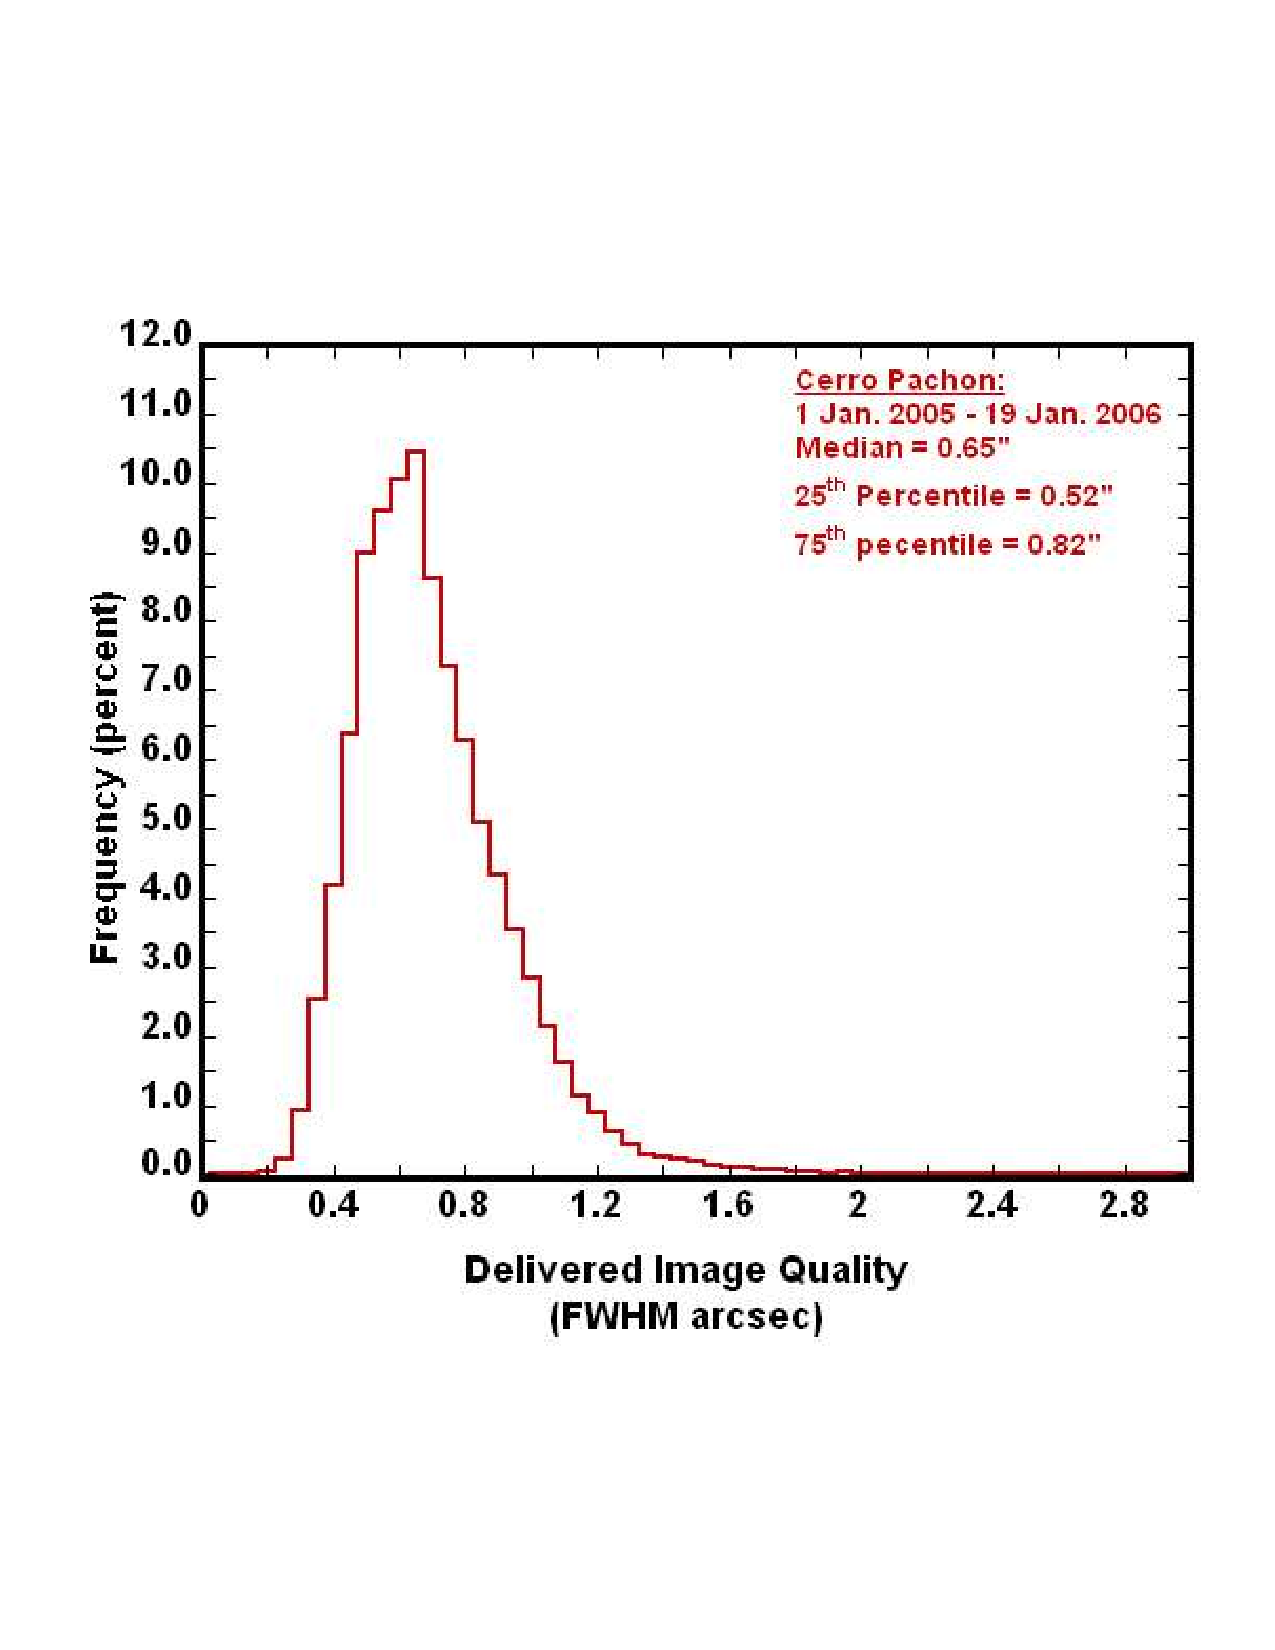
\includegraphics[width=1.0\hsize,clip]{seeing2.pdf}
\caption{
The image quality distribution measured at the Cerro Pach\'{o}n site using a
DIMM (differential image motion monitor) at $\lambda$ = 500 nm, and corrected 
using an outer scale parameter of 30 m over an 8.4 m aperture. For details 
about the outer scale correction see Tokovinin (2002). The observed distribution 
is well described by a log-normal distribution, with the parameters shown in 
the figure.} 
\label{Fig:seeing}
\end{figure}

\subsubsection{A Summary and Synthesis of Science-driven Constraints on Data Properties}

The goals of all the science programs discussed above 
(and many more, of course) can be accomplished by satisfying the 
minimal constraints listed below. For a more elaborate listing
of various constraints, including detailed specification of 
various probability distributions, please see the LSST Science
Requirements Document\footnote{http://www.lsst.org/files/docs/SRD.pdf}
and the LSST Science Book. 

\begin{enumerate}
\item  {\it The single visit depth} should reach $r\sim24.5$. This limit is
   primarily driven by the NEO survey, variable sources (e.g., SN,
   RR Lyrae stars), and by proper motion and trigonometric parallax 
   measurements for stars. Indirectly, it is also driven by the
   requirements on the coadded survey depth and the minimum number of 
   exposures required by WL science. 
\item  {\it Image quality} should maintain the limit set by the 
     atmosphere (the median free-air seeing is 0.65 arcsec in the $r$ band 
     at the chosen site, see Fig.~\ref{Fig:seeing}),
     and not be degraded appreciably by the hardware. In addition to stringent 
     constraints from weak lensing, good image quality is driven by the 
     required survey depth for point sources and by image differencing
     techniques. 
\item  {\it Photometric repeatability} should achieve 5 mmag precision
     at the bright end, with zeropoint stability across the sky of 10 mmag
     and band-to-band calibration errors not larger than 5 mmag.
     These requirements are driven by the photometric redshift accuracy,
     the separation of stellar populations, detection of low-amplitude variable
     objects (such as eclipsing planetary systems), and the search for
     systematic effects in type Ia supernova light curves.
\item  {\it Astrometric precision} should maintain the limit set by 
     the atmosphere, of about 10 mas per visit at the bright end
     (on scales below 20 arcmin). This precision is driven by the desire to 
     achieve a proper motion accuracy of 0.2 mas yr$^{-1}$ and parallax accuracy of 
     1.0 mas over the course of a 10-year survey (see \S \ref{Sec:apSize}).
\item  {\it The single visit exposure time} (including both exposures in a 
    visit, which are required for cosmic ray rejection) should be less than about a minute 
    to prevent trailing of fast moving objects and to aid control 
    of various systematic effects induced by the atmosphere. It should
    be longer than $\sim$20 seconds to avoid significant efficiency losses due to
    finite readout, slew time, and read noise.
\item  {\it The filter complement} should include at least six filters
    in the wavelength range limited by atmospheric absorption and 
    silicon detection efficiency (320--1050 nm), with roughly
    rectangular filters and no large gaps in the coverage, in order
    to enable robust and accurate photometric redshifts and stellar typing. An 
    SDSS-like $u$ band (Fukugita et al. 1996) is extremely important for separating 
    low-redshift quasars from hot stars, and for estimating the metallicities of 
    F/G main sequence stars. A bandpass with an effective wavelength of
    about 1 micron  would enable studies of sub-stellar objects, high-redshift 
    quasars (to redshifts of $\sim$7.5), and regions of the Galaxy that are obscured 
    by interstellar dust.
\item  {\it The revisit time distribution} should enable determination of
   orbits of Solar System objects and sample SN light curves every few days, 
   while accommodating constraints set by proper motion and trigonometric 
   parallax measurements.
\item  {\it The total number of visits} of any given area of sky, when accounting for all 
   filters, should be of the order of 1,000, as mandated by WL science, the
   NEO survey, and proper motion and 
   trigonometric parallax measurements. Studies of transient sources 
   also benefit from a large number of visits.
\item  {\it The coadded survey depth} should reach 
    $r\sim27.5$, with sufficient signal-to-noise ratio in other bands
    to address both extragalactic and Galactic science drivers.
\item  {\it The distribution of visits per filter} should enable 
   accurate photometric redshifts, separation of stellar populations,
   and sufficient depth to enable detection of faint extremely red
   sources (e.g., brown dwarfs and high-redshift quasars). Detailed simulations of 
   photometric redshift estimates
   suggest an approximately flat distribution of visits among bandpasses
   (because the system throughput and atmospheric properties are 
    wavelength dependent, the achieved depths are different in different
    bands). The adopted time allocation
   (see Table 1) includes a slight preference to the $r$ and $i$ bands because of their
   dominant role in star/galaxy separation and weak lensing measurements. 
\item  {\it The distribution of visits on the sky} should extend over
   at least $\sim$20,000 deg$^2$ to obtain the required number of galaxies
   for WL studies, with attention paid to include ``special''
   regions such as the Ecliptic and Galactic planes, and the Large and Small
   Magellanic Clouds. 
\item  {\it Data processing, data products and data access} should enable 
   efficient science analysis without a significant impact on the final 
   uncertainties. To enable a fast and efficient response to
   transient sources, the processing latency should be less than a minute,
   with a robust and accurate preliminary classification 
   of reported transients.
\end{enumerate}

Remarkably, even with these joint requirements, none of the 
individual science programs is severely over-designed, i.e., despite 
their significant scientific diversity, these programs are highly 
compatible in terms of desired data characteristics. Indeed, any one
of the four main science drivers could be removed, and the remaining 
three would still yield very similar requirements for most system 
parameters. As a result, the LSST system can adopt a highly 
efficient survey strategy where {\it a single dataset serves most science
programs} (instead of science-specific surveys executed in series). 
One can view this project as {\it massively parallel astrophysics}.
The vast majority (about 90\%) of the observing time will be devoted to 
a deep-wide-fast survey mode, with the remaining 10\% 
allocated to special programs which will also address multiple science 
goals. Before describing these surveys in detail, we discuss the main 
system parameters. 


\begin{table}
\caption{The LSST Baseline Design and Survey Parameters}
\begin{tabular}{|l|l|}
\hline  
   Quantity                         &     Baseline Design Specification    \\
\hline  
Optical Config.                     &  3-mirror modified Paul-Baker        \\
Mount Config.                       &  Alt-azimuth          \\
Final f-ratio, aperture             &  f/1.234, 8.4 m                \\
Field of view, \'etendue            &  9.6 deg$^2$,   319 m$^2$deg$^2$     \\
Plate Scale                         &  50.9 $\mu$m/arcsec (0.2'' pix)  \\
Pixel count                         &  3.2 Gigapix  \\
Wavelength Coverage                 &  320 -- 1050 nm, $ugrizy$                        \\
Single visit depths$^a$ (5$\sigma$) &  23.9, 25.0, 24.7, 24.0, 23.3, 22.1  \\
Mean number of visits               &  56, 80, 184, 184, 160, 160  \\ 
Final (coadded) depths$^a$          &  26.1, 27.4, 27.5, 26.8, 26.1, 24.9 \\
\hline                         
\end{tabular}
\\ \vskip 0.05in
$^a$ The listed values for 5$\sigma$ depths in the $ugrizy$ bands, respectively, 
are AB magnitudes, and correspond to point sources and zenith observations
(about 0.2 mag loss of depth is expected for realistic airmass distributions). 
See Table 2 for more details.   
\vskip 0.2in          
\end{table}



\subsection{The Main System Design Parameters} 

Given the minimum science-driven constraints on the data properties listed 
in the previous section, we now discuss how they are translated into
constraints on the main system design parameters: the aperture size, 
the survey lifetime, the optimal exposure time, and the filter complement. 


\subsubsection{ The Aperture Size }
\label{Sec:apSize}
The product of the system's \'etendue and the survey lifetime, for given
observing conditions, determines
the sky area that can be surveyed to a given depth, where the \'etendue is
the product of the primary mirror area and the field-of-view area. The 
LSST field-of-view area is maximized to its practical limit, $\sim$10 deg$^2$, 
determined by the requirement that the delivered image quality be dominated 
by atmospheric seeing at the chosen site (Cerro Pach\'{o}n in Northern Chile). 
A larger field-of-view would lead to unacceptable deterioration of the 
image quality. This constraint leaves the primary mirror diameter and survey lifetime 
as free parameters. The adopted survey lifetime of 10 years is a compromise 
between a shorter time that leads to an excessively large and expensive mirror (15m for a 
3 year-long survey and 12m for a 5-year long survey) and not as effective proper motion
measurements, and a smaller telescope that would require more time to complete the 
survey, with the associated increase in operations cost.

The primary mirror size is a function of the required survey depth and the 
desired sky coverage. By and large, the anticipated science outcome scales 
with the number of detected sources. For practically all astronomical source 
populations, in order to maximize the number of detected sources, it is more 
advantageous to maximize the area first, and then 
the detection depth\footnote{ 
If the total exposure time is doubled and used to double the survey area, 
the number of sources increases by a factor of two. If the survey 
area is kept fixed, the increased exposure time will result in 
$\sim$0.4 mag deeper data (see eq.~\ref{m5}). For cumulative source 
counts described by $\log(N) = C + k*m$, the number of sources
will increase by more than a factor of two only if $k>0.75$. 
Apart from low-redshift quasars ($z<2$), practically all populations 
have $k$ at most 0.6 (the so-called Euclidean counts), and faint stars 
and galaxies have $k<0.5$. For more details, please see Nemiroff
(2003).}. For this reason, the sky area for the main survey is 
maximized to its practical limit, 20,000 deg$^2$, determined by the 
requirement to avoid large airmasses ($X<1.5$, where approximately $X={\rm sec}(\theta)$ 
and $\theta$ is the zenith distance), which would substantially 
deteriorate the image quality and the survey depth (see eq.~\ref{m5}). 

With the adopted field-of-view area, the sky coverage and the survey lifetime 
fixed, the primary mirror diameter is fully driven by the required survey 
depth. There are two depth requirements: the final (coadded) survey depth, 
$r\sim27.5$, and the depth of a single visit, $r\sim24.5$. The two 
requirements are compatible if the number of visits is several hundred
(per band), which is in good agreement with independent science-driven 
requirements on the latter.  

The required coadded survey depth provides a direct constraint, 
independent of the details of survey execution such as the exposure time per visit, 
on the minimum effective primary mirror diameter of 6.5m, as illustrated in 
Fig.~\ref{Fig:coaddDepth}. 



\subsubsection{ The Optimal Exposure Time }

The single visit depth depends on both the primary mirror diameter and the
chosen exposure time, $t_{\rm vis}$. In turn, the exposure time 
determines the time interval to revisit a given sky position and the total 
number of visits, and each of these quantities has its own science 
drivers. We summarize these simultaneous constraints in terms of the 
single-visit exposure time:
\begin{itemize}
\item  The single-visit exposure time should not be longer than about a minute to 
         prevent trailing of fast Solar System moving objects, and to enable efficient
         control of atmospheric systematics.
\item  The mean revisit time (assuming uniform cadence) for a given position 
         on the sky, $n$, scales as 
\begin{equation}
  n = \left( {t_{\rm vis} \over 10  \, {\rm sec}} \right)
      \left( { A_{\rm sky} \over 10,000  \, {\rm deg}^2} \right)
      \left( {10 \, {\rm deg}^2 \over  A_{\rm FOV}} \right) {\rm days},
\end{equation}
where two visits per night are assumed (required for efficient detection of 
solar system objects, see below), and the losses for realistic observing conditions 
have been taken into account (with the aid of the Operations Simulator described below). 
Science drivers such as SN and moving objects in the Solar System require 
that $n<4$ days, or equivalently $t_{vis} < 40$ seconds for the nominal values 
of $A_{sky} $ and $A_{FOV}$. 
\item  The number of visits to a given position on the sky, $N_{visit}$,
%again 
with losses for realistic observing conditions taken into account,
is given by
\begin{equation}
      N_{visit} = \left( {3000 \over n} \right)
                    \left( { T \over 10 \, {\rm yr}} \right).
\end{equation}
The requirement $N_{visit}>800$ again implies that $n<4$ and 
$t_{vis} < 40$ seconds if the survey lifetime, $T \sim 10$ years. 
\item  These three requirements place a firm upper limit on the 
optimal visit exposure time of $t_{vis} < 40$ seconds. Surveying 
efficiency (the ratio of open-shutter time to the total
time spent per visit) considerations place a lower limit on 
$t_{vis}$ due to finite detector read-out and telescope slew time (the longest 
acceptable read-out time is set to 2 seconds, and the slew and 
settle time is set to 5 seconds, including the read-out time
for the second exposure in a visit):
\begin{equation}
      \epsilon = \left( {t_{vis} \over t_{vis} + 7 \, {\rm sec}}\right).
\end{equation}
To maintain efficiency losses below 30\% (i.e., at least below the 
limit set by the weather patterns), and to minimize the read noise
impact, $t_{vis} > 20$ seconds is required. 
\end{itemize}

Taking these constraints simultaneously into account, as summarized in 
Fig.~\ref{Fig:singleDepth}, 
yielded the following reference design:
\begin{enumerate}
\item A primary mirror effective diameter of $\sim$6.5m. With the adopted optical 
design, described below, this effective diameter corresponds to a geometrical diameter 
of $\sim$8m. Motivated by characteristics of the existing equipment at the
Steward Mirror Laboratory, which is fabricating the primary mirror, the adopted
geometrical diameter is set to 8.4m. 
\item A visit exposure time of 30 seconds (using two 15 second exposures
to efficiently reject cosmic rays), yielding $\epsilon=77$\%.
\item A revisit time of 3 days on average for 10,000 deg$^2$ of sky, 
  with two visits per night.
\end{enumerate}

\begin{figure}[t]
\vskip -0.5in
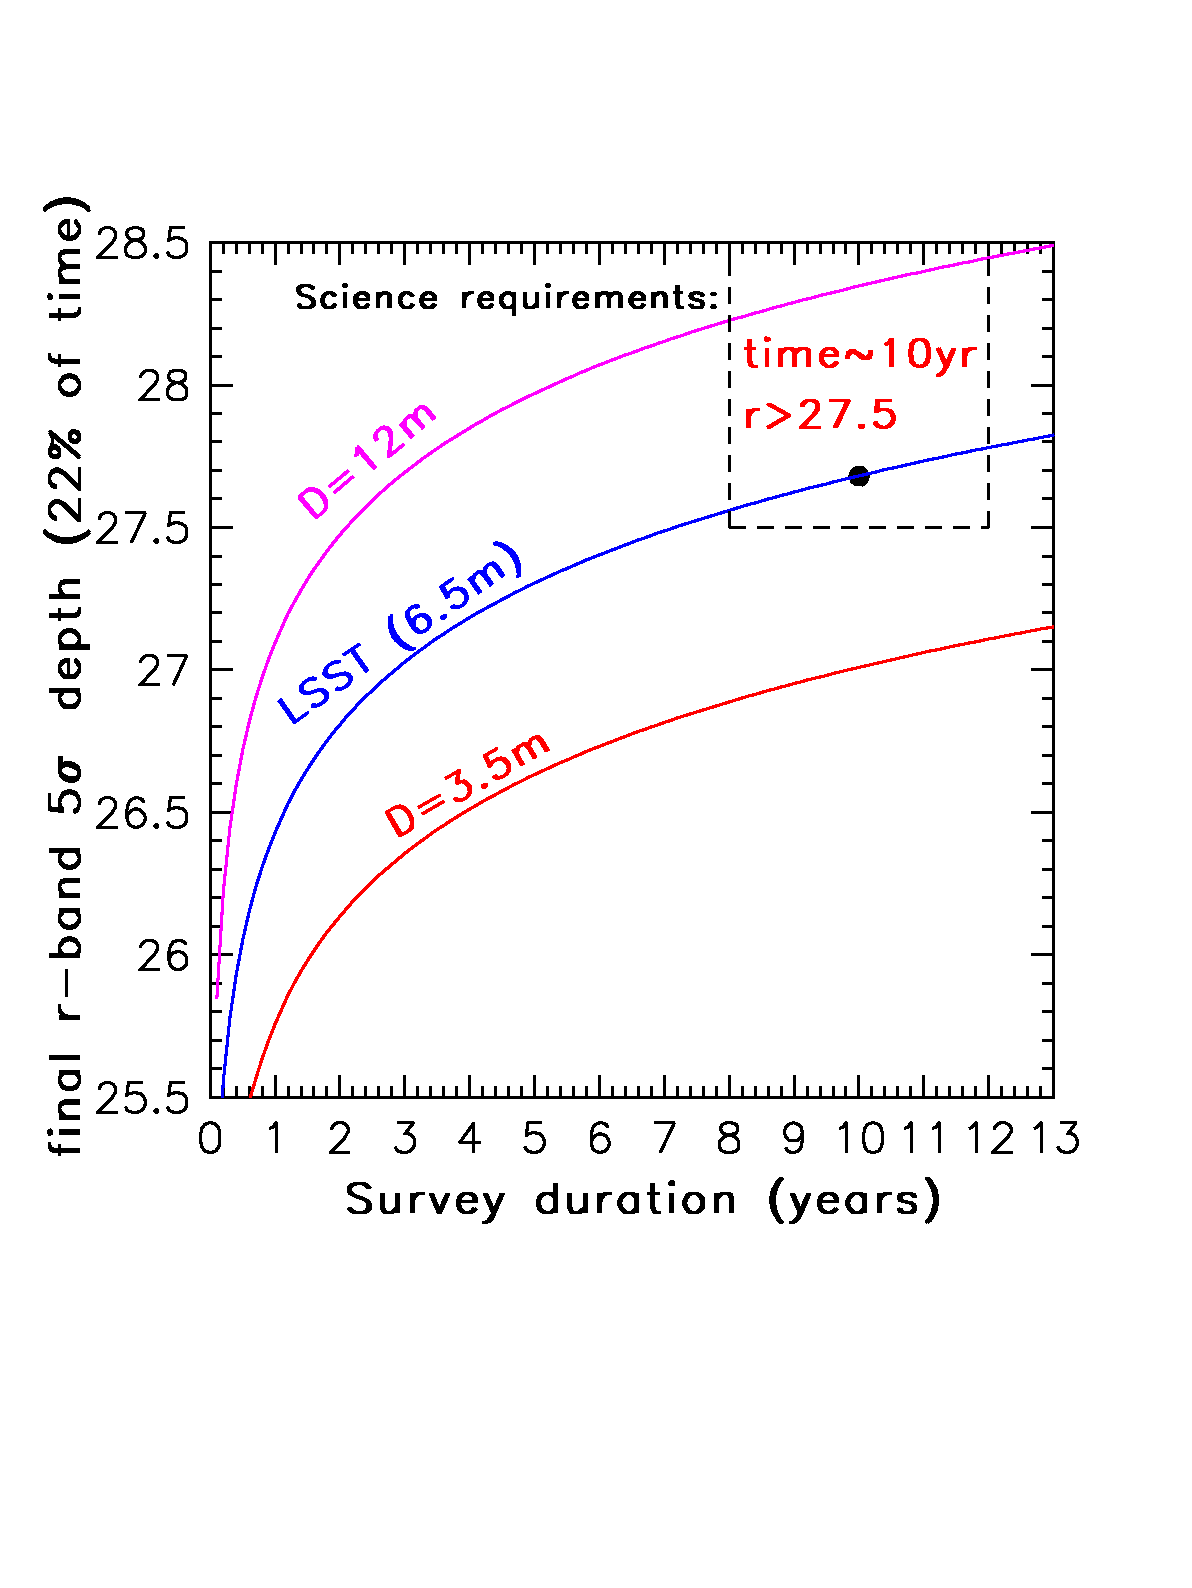
\includegraphics[width=1.1\hsize,clip]{coaddedDepth.pdf}
\vskip -1.1in
\caption{The coadded depth in the $r$ band (AB magnitudes) vs. the effective aperture and 
the survey lifetime. It is assumed that 22\% of the total observing time (corrected for
weather and other losses) is allocated for the $r$ band, and that the ratio of 
the surveyed sky area to the field-of-view area is 2,000.} 
\label{Fig:coaddDepth}
\end{figure}

\begin{figure}[t]
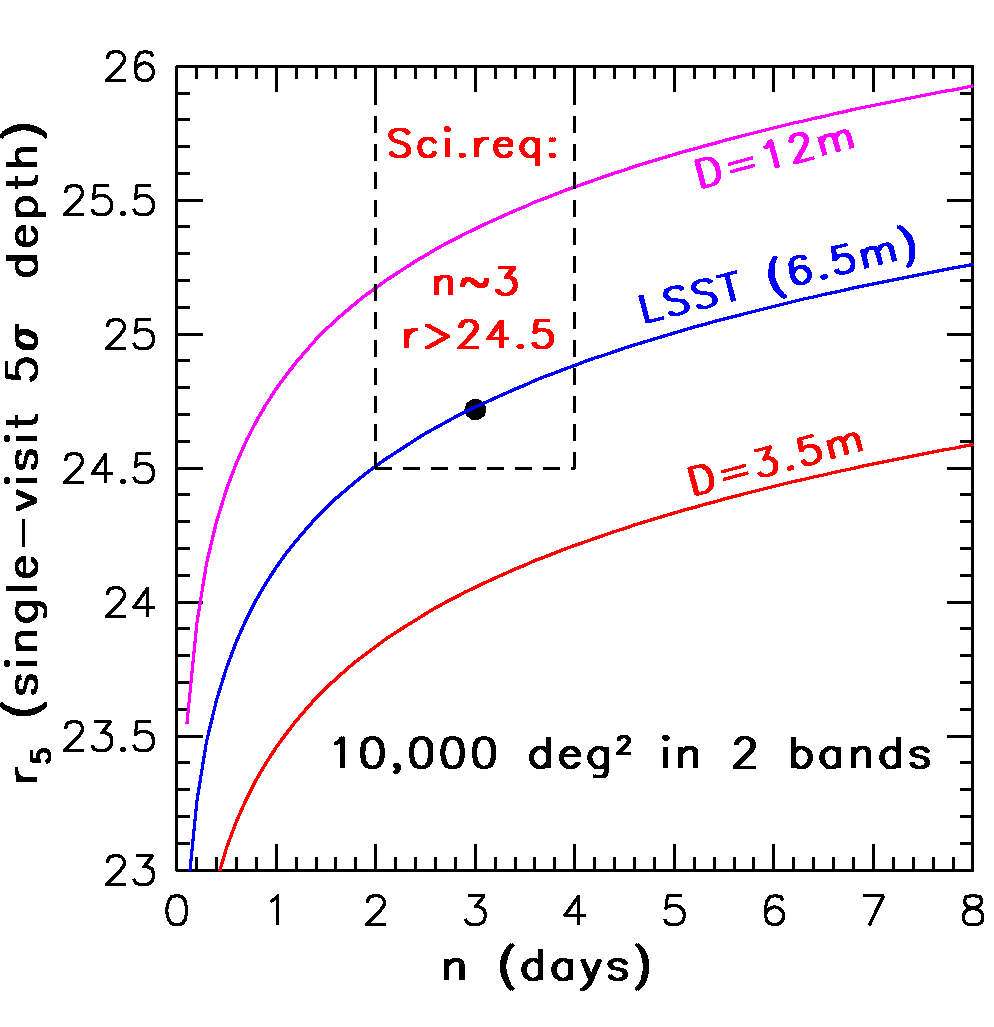
\includegraphics[width=1.0\hsize,clip]{singleDepth.pdf}
\caption{The single-visit depth in the $r$ band (5$\sigma$ detection for 
point sources, AB magnitudes) vs. revisit time, $n$ (days), as a function of 
the effective aperture size. With a coverage of 10,000 deg$^2$ in two bands, 
the revisit time directly constrains the visit exposure time, $t_{vis}=10\,n$ 
seconds. In addition to direct constraints on optimal exposure time, $t_{vis}$ 
is also driven by requirements on the revisit time, $n$, the total number of visits 
per sky position over the survey lifetime, $N_{visit}$, and the survey efficiency,
$\epsilon$ (see eqs.1-3). Note that these constraints result in a fairly narrow range of 
allowed $t_{vis}$ for the main deep-wide-fast survey.} 
\label{Fig:singleDepth}
\end{figure}

To summarize, the chosen primary mirror diameter is the {\it minimum}
diameter that simultaneously satisfies the depth ($r\sim24.5$ for single visit and 
$r\sim27.5$ for coadded depth) and cadence (revisit time of 3-4 days, 
with 30 seconds per visit) constraints described above.

\subsection{System Design Trade-offs}

We note that the Pan-STARRS project (Kaiser et al. 2002), with similar science
goals as LSST, has adopted a distributed aperture design, where the total
system \'etendue is 
a sum of \'etendue values for an array of small telescopes (the prototype
PS1 telescope has an \'etendue of 1/24$^{th}$ of the LSST's \'etendue). 
Similarly, the LSST system could perhaps be made as two smaller copies with 
6m mirrors, or 4 copies with 4m mirrors, or 16 copies with 2m mirrors. Each 
of these clones would have to have its own 3 Gigapixel camera (see below), and 
given the added risk and complexity (e.g., maintenance, data processing), the monolithic 
design seems advantageous for a system with such a large \'etendue as LSST. 

It is informative to consider the tradeoffs that would be required 
for a system with a smaller aperture, if the science requirements were
to be maintained. For this comparison, we consider a four-telescope version of
the Pan-STARRS survey (PS4). With an \'etendue about 6 times smaller 
than that of LSST (effective diameters of 6.5m and 3.0m, and a field-of-view area 
of 9.6 deg$^2$ vs. 7.2 deg$^2$), and all observing conditions being equal,
the PS4 system could in principle use an identical cadence as that of LSST. The
main difference in the datasets would be a faint limit shallower by about 
1 mag in a given survey lifetime. As a result, for Euclidean populations the 
sample sizes would go down by a factor of 4, while for shallower populations (e.g.,
galaxies around redshift of 1) the samples would be smaller by about a factor 2-3. 
The distance limits for nearby sources, such as Milky Way stars, would drop to
60\% of their corresponding LSST values, and the NEO completeness level mandated by
the U.S. Congress would not be reached.  

If instead the survey coadded depth were to be maintained, then the survey sky 
area would have to be 6 times smaller ($\sim$3,500 deg$^2$). If the
survey single-visit depth were to be maintained, then the exposure
time would have to be about 6 times longer (ignoring the slight difference
in the field-of-view area and simply scaling by the \'etendue ratio), 
resulting in non-negligible trailing losses for solar system objects, 
and either 
i) a factor of six smaller sky area observed within $n=3$ days, or 
ii) the same sky area revisited every $n=18$ days. 
Given these conflicts, one solution would be to split the observing time and 
allocate it to individual specialized programs (e.g., large sky area vs. 
deep coadded data vs. deep single-visit data vs. small $n$ data, etc.), 
as considered by the PS1 Consortium\footnote{More information about 
Pan-STARRS is available from http://pan-starrs.ifa.hawaii.edu.}. 

In summary,
{\it given the science requirements as stated here, there is a
minimum \'etendue of $\sim$300 deg$^2$m$^2$ which enables our seemingly
disparate science goals to be addressed with a single data set.}
A system with a smaller \'etendue would require separate specialized surveys
to address the science goals, which results in a loss of surveying
efficiency\footnote{The converse is also true: for every \'etendue
there is a set of optimal science goals that such a system can 
address with a high efficiency.}. The LSST is designed to reach this 
minimum \'etendue for the science goals stated in its Science Requirements 
Document. 



\subsection{  The Filter Complement }

The LSST filter complement ($ugrizy$, see Fig.~\ref{Fig:filters}) is modeled after the Sloan
Digital Sky Survey 
(SDSS) system (Fukugita et al. 1996) because of its demonstrated success in a wide
variety of applications, including photometric redshifts of galaxies (Budav\'{a}ri
et al. 2003), separation of stellar populations (Lenz et al. 1998; Helmi et al. 2003), 
and photometric selection of quasars (Richards et al. 2002). The extension of the 
SDSS system to longer wavelengths
(the $y$ band at $\sim$1 micron) is driven by the increased effective redshift 
range achievable with the LSST due to deeper imaging, the desire to study sub-stellar 
objects, high-redshift quasars, and regions of the Galaxy that are obscured by
interstellar dust, and
the scientific opportunity enabled by modern CCDs with high quantum efficiency 
in the near infrared.  


\begin{figure}
\hskip -0.13in
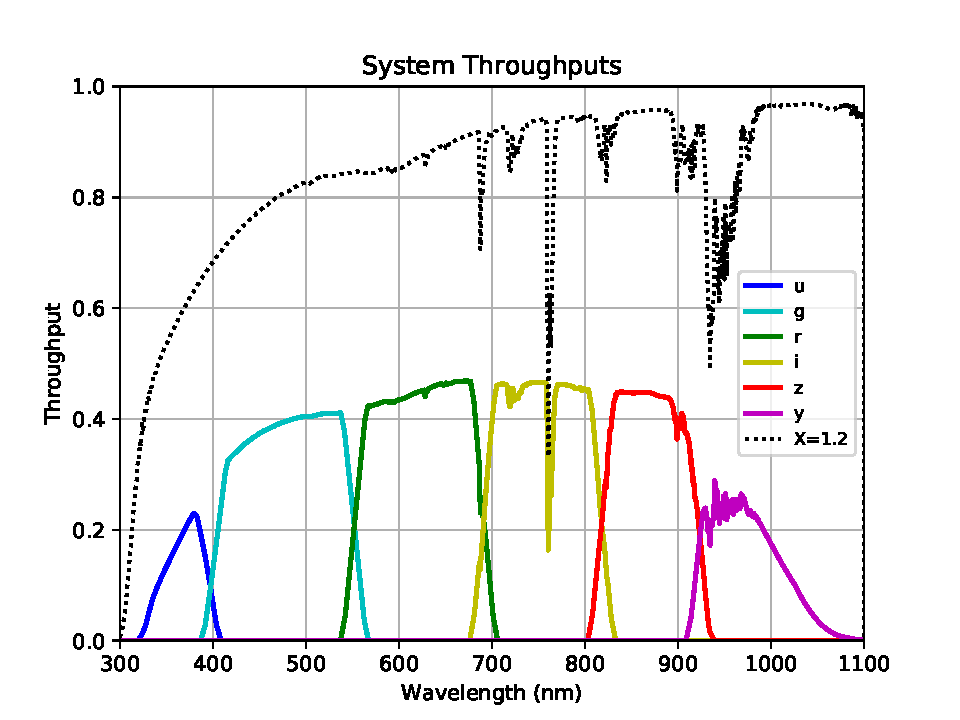
\includegraphics[width=1.1\hsize,clip]{filters_y4.pdf}
\caption{The {\it current} design of the LSST bandpasses. 
The vertical axis shows the total throughput. The computation includes the atmospheric 
transmission (assuming an airmass of 1.2 at an altitude of $\sim$56 deg., dotted line), optics, and the 
detector sensitivity. The detailed design of the $y$ band is still being optimized; the figure 
shows the so-called $y_4$ version which includes the atmospheric water absorption feature 
at $\sim$0.95 $\mu$m.} 
\label{Fig:filters}
\end{figure}


The chosen filter complement corresponds to a design ``sweet spot''. We have 
investigated the possibility of replacing the $ugrizy$ system with a
filter complement that includes only five filters. For example, each filter
width could be increased by 20\% over the same wavelength range (neither a
shorter wavelength range, nor gaps in the wavelength coverage are desirable 
options), but this option is not satisfactory. Placing the red edge of the $u$ 
band blueward of the Balmer break allows optimal separation of stars and
quasars, and the telluric water absorption feature at 9500\AA\
effectively defines the blue edge of the $y$ band. Of the remaining four
filters ($griz$), the $g$ band is already quite wide. As a last option, the 
$riz$ bands could be redesigned as two wider bands. However, this option is also 
undesirable because the $r$ and $i$ bands are the primary bands for weak
lensing studies and for star/galaxy separation, and chromatic atmospheric
refraction would worsen the point spread function for a wider bandpass. 



\subsection{ The Calibration Methods }


\begin{figure}
\hskip -0.12in
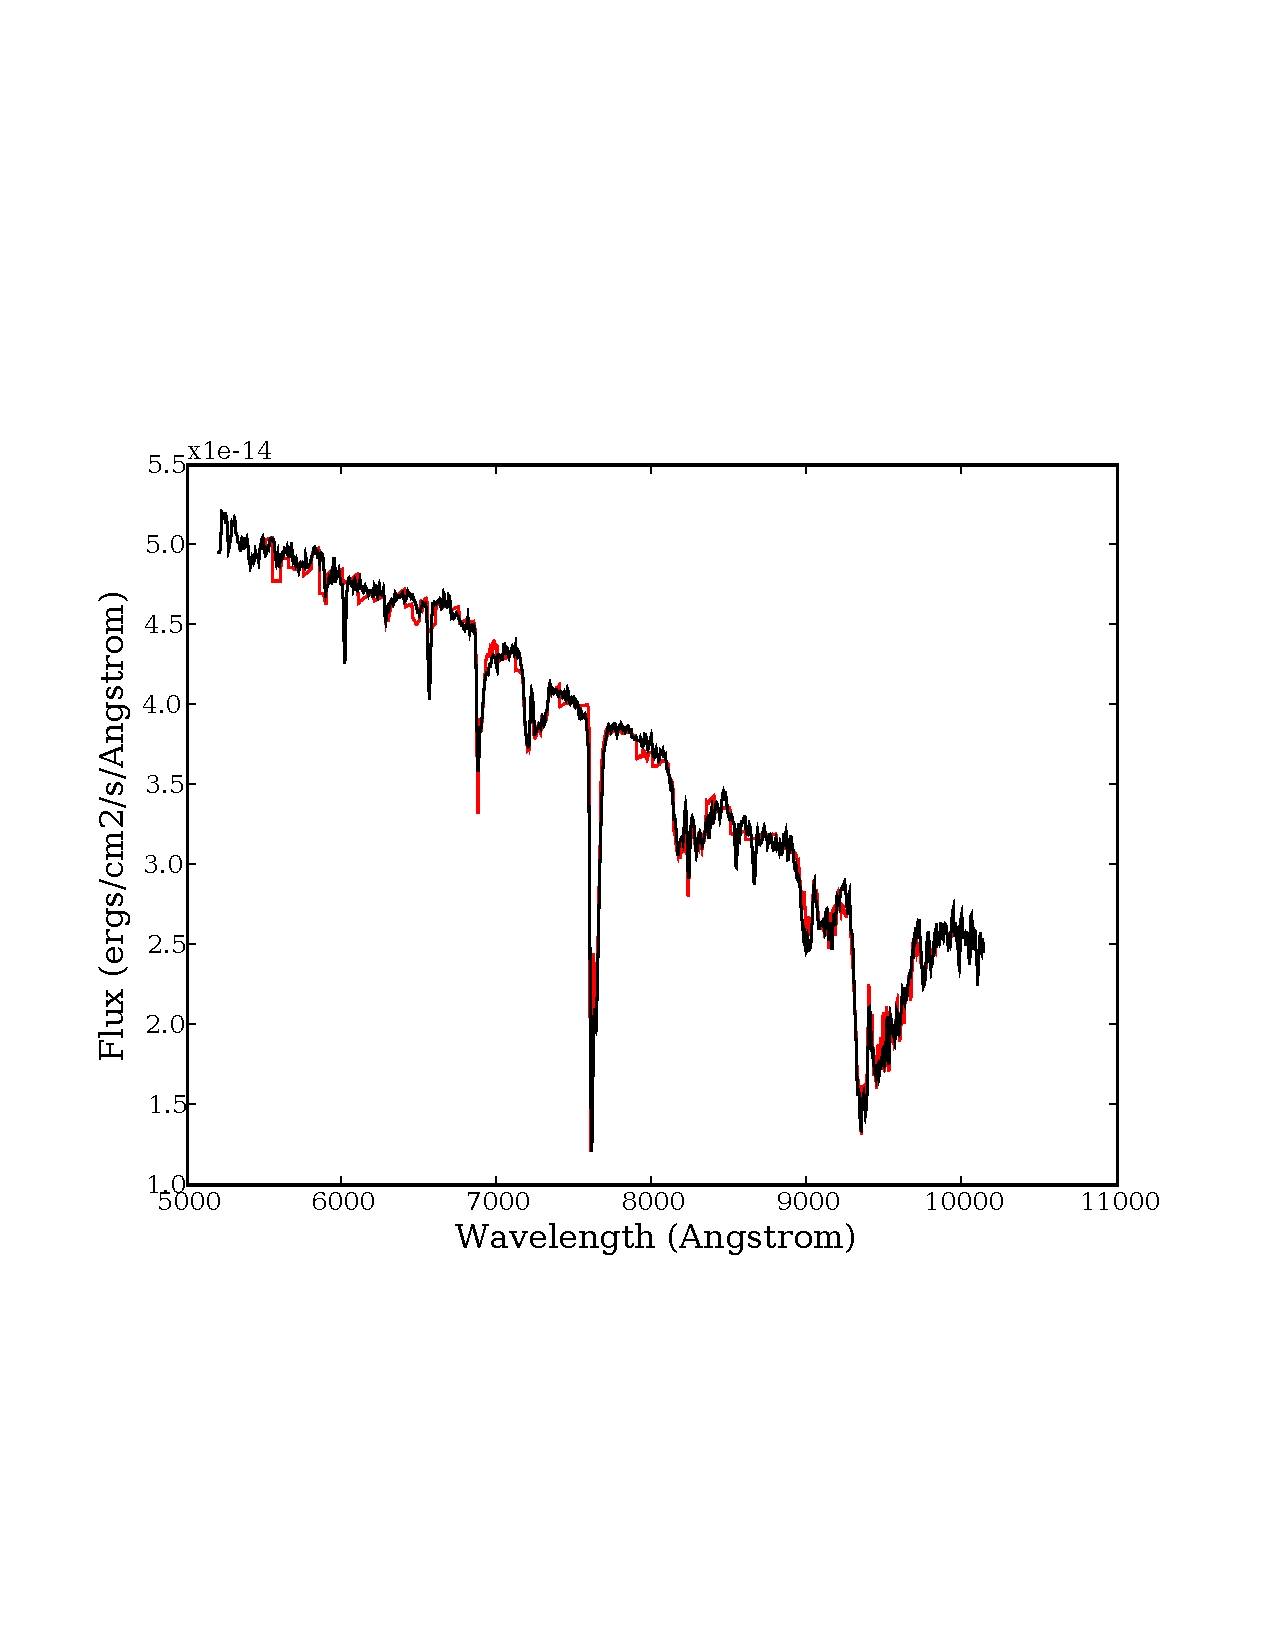
\includegraphics[width=1.1\hsize,clip]{modtran1.pdf}
\caption{An example of determination of the atmospheric opacity by 
simultaneously fitting a three-parameter stellar model SED (Kurucz 1979) and 
six physical parameters of a sophisticated atmospheric model (MODTRAN, Anderson 
et al. 1999) to an observed F-type stellar spectrum ($F_\lambda$). The black 
line is the observed spectrum and the red line is the best fit. Note that the 
atmospheric water feature around 0.9-1.0 $\mu$m is exquisitely well fit. 
The components of the best-fit atmospheric opacity are shown in 
Fig.~\ref{Fig:modtran2}. Adapted from Burke et al. (2007).}
\label{Fig:modtran1}
\end{figure}

\begin{figure}
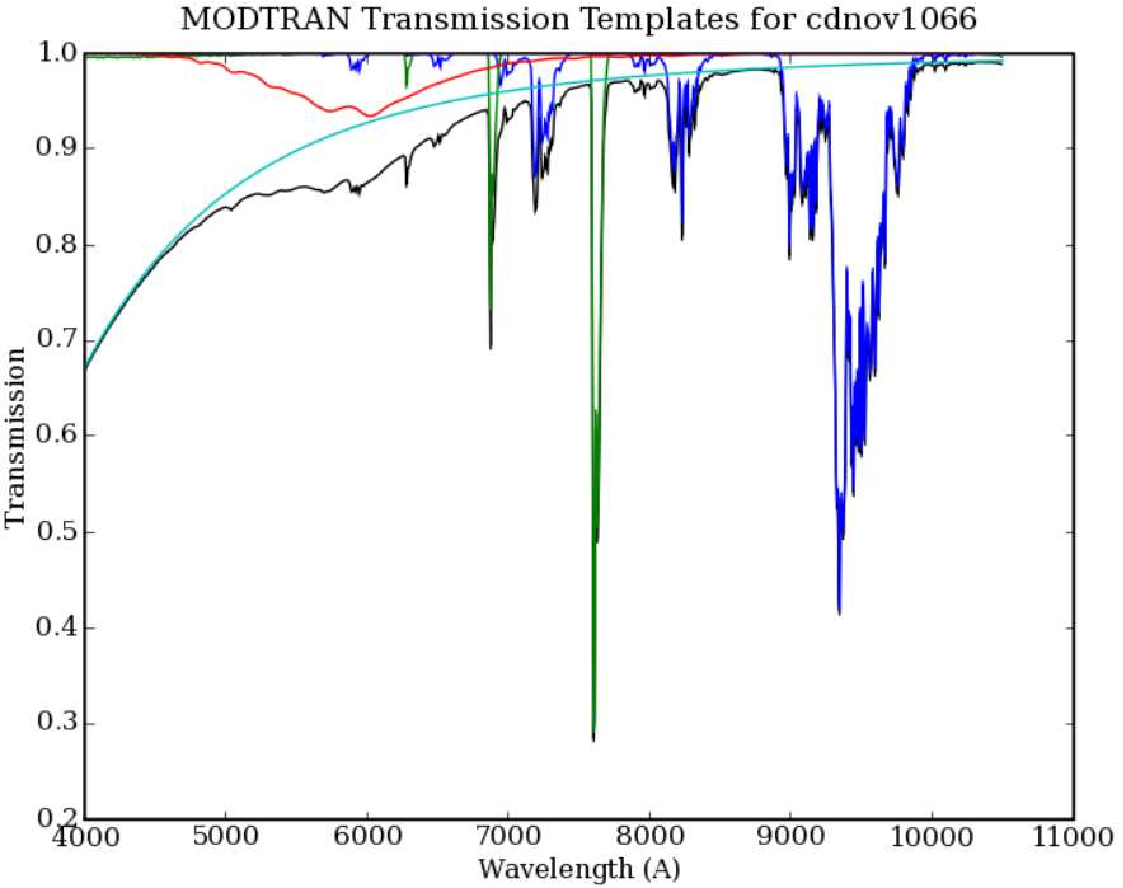
\includegraphics[width=1.0\hsize,clip]{modtran2.pdf}
\caption{The components of the best-fit atmospheric opacity used to
model the observed stellar spectrum shown in Fig.~\ref{Fig:modtran1}.
The atmosphere model (MODTRAN, Anderson et al. 1999) includes six
components: water vapor (blue), oxygen and other trace molecules
(green), ozone (red), Rayleigh scattering (cyan), a gray term
with a transmission of 0.989 (not shown) and an aerosol contribution
proportional to $\lambda^{-1}$ and extinction of 1.3\% at $\lambda$=0.675 \mic\
(not shown). The black line shows all six components combined.
Adapted from Burke et al. (2007).}
\label{Fig:modtran2}
\end{figure}


Precise determination of the point spread function across each image, 
accurate photometric and astrometric calibration, and continuous monitoring 
of system performance and observing conditions will be needed to reach the 
full potential of the LSST mission. Extensive precursor data including the 
massive SDSS dataset and our own data obtained using telescopes close to 
the LSST site of Cerro Pach\'{o}n (e.g., the SOAR and Gemini South telescopes), 
as well as telescopes of similar aperture (e.g., Subaru), indicate that the 
photometric and astrometric accuracy will be limited not by our instrumentation 
or software, but rather by atmospheric effects. Active optics will assure 
superb image quality. 

The required 1\% photometric accuracy is driven by our requirements 
on the photometric redshift accuracy, the separation of stellar populations, 
the ability to detect low-amplitude variable objects, and the search for 
systematic effects in type Ia supernova light curves. SDSS data 
taken in good photometric conditions have indeed reached the LSST requirements
(Padmanabahn et al. 2008), although measurements with ground-based telescopes 
typically produce data with errors a factor of two or so larger. Analysis of
repeated SDSS scans obtained in varying observing conditions demonstrates that data
obtained in traditionally non-photometric conditions can also be calibrated with
sufficient accuracy (Ivezi\'{c} et al. 2007b). 

The LSST calibration plan builds on experience gained from the SDSS survey. 
The planned calibration process decouples the establishment of a stable and uniform internal 
relative calibration from the task of assigning absolute optical flux to 
celestial objects. The latter effort requires determination of a small 
number of factors appropriate for the accumulated multi-epoch data set. 
Celestial sources will be used to define the internal photometric system and 
to monitor stability and uniformity of photometric data. There will be 
$>$100 main-sequence stars with $17<r<20$ per detector (14$\times$14 arcmin$^2$) 
even at high Galactic latitudes. Standardization of photometric scales will be 
achieved through direct observation of stars with well-understood spectral 
energy distributions (SEDs). 

While the primary source of data used for photometric calibration will be 
science images taken with the main telescope, these images alone will be 
insufficient to fully characterize instrumental and atmospheric temporal and 
spatial variations that can affect photometric measurements. Auxiliary 
instrumentation, including a 1.5m calibration telescope, will provide the 
calibration parameters needed for image 
processing, to calibrate the instrumental response of the LSST hardware
(Stubbs \& Tonry 2006), and to measure the atmospheric optical depth as 
a function of wavelength along the LSST line of sight (Stubbs et al. 2007; 
see Figs.~\ref{Fig:modtran1} and \ref{Fig:modtran2}). 


\subsection{     The LSST  Reference Design    }

We briefly describe the reference design for the main LSST system components. 
Detailed discussion of the flow-down from science requirements to system 
design parameters, and extensive system engineering analysis can be 
found in the LSST Science Book (Ch.~2--3). 

\begin{figure}
\vskip -0.5in
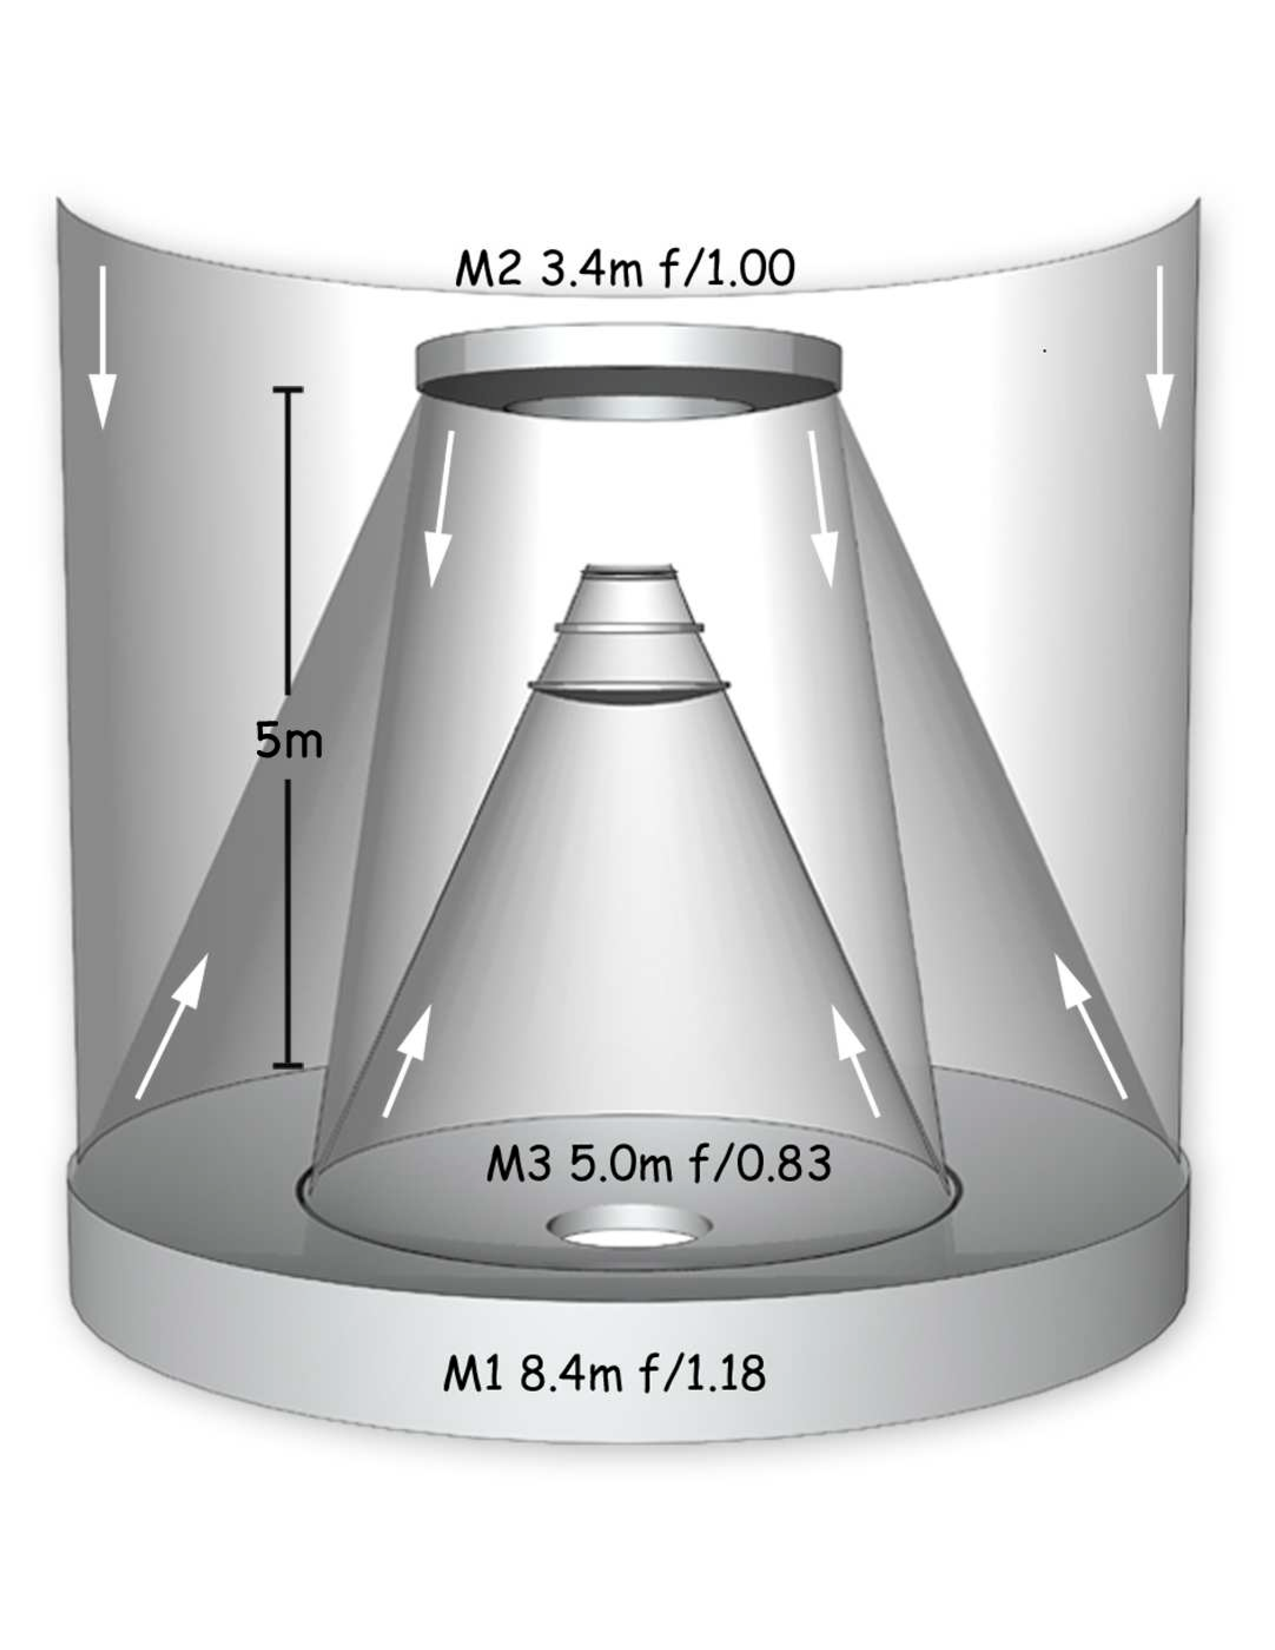
\includegraphics[width=1.0\hsize,clip]{mirrors.pdf}
\vskip -0.5in
\caption{The LSST baseline optical design with its unique 
monolithic mirror: the primary and tertiary mirrors are positioned such 
that they form a continuous compound surface, allowing them to be polished 
into a single substrate.}
\label{Fig:optics}
\end{figure}



\subsubsection{ Telescope and Site}

The large LSST \'etendue is achieved in a novel three-mirror design (modified
Paul-Baker; Angel, Lesser \& Sarlot 2000) with a very fast $f$/1.234 beam. The optical 
design has been optimized to yield a large field of view (9.6 deg$^2$), 
with seeing-limited image quality, across a wide wavelength band (320--1050
nm). Incident light is collected by the primary mirror, which is an annulus
with an outer diameter of 8.4 m and inner diameter of 5.0m (an effective diameter of 
6.5m), then reflected to a 3.4m convex secondary, onto a 5m concave tertiary, and finally 
into three refractive lenses in a camera (see Fig.~\ref{Fig:optics}). This is achieved 
with an innovative approach that positions the tertiary mirror inside the primary 
mirror annulus ring, making it possible to fabricate the mirror pair from a 
single monolithic blank using borosilicate technology. The secondary is 
a thin meniscus mirror, fabricated from an ultra-low expansion material. All 
three mirrors will be actively supported to control wavefront distortions 
introduced by gravity and environmental stresses on the telescope. 
The primary-tertiary mirror and the secondary mirror were 
cast\footnote{http://www.lsst.org/News/enews/m1m3-1004.html}  in 2008 and 2009,
and the primary-tertiary mirror is currently being polished. 

The telescope mount is a compact, stiff structure with a fundamental frequency of 
nearly 10 Hz, which is crucial for achieving the required fast slew-and-settle times
(see Fig.~\ref{Fig:telescope}). The telescope sits on a concrete pier within a 
carousel dome that is 30 m in diameter (Fig.~\ref{Fig:observatory}). The dome has 
been designed to reduce dome seeing (local air turbulence that can distort images) 
and to maintain a uniform thermal environment over the course of the night. 
The LSST Observatory will be sited atop Cerro Pach\'{o}n in northern Chile,
near the Gemini South and SOAR telescopes\footnote{Coordinates listed in older versions 
of this paper were incorrect. We thank E. Mamajek for pointing this error to us.} 
% old, WRONG: (latitude: S 30$^\circ$ 10$'$ 20.1$"$; longitude: W 70$^\circ$ 48$'$ 0.1$"$; elevation: 2123 m; 
% from Mamajek (2012, arXiv:1210.1616, Table 3, GPS values): 
(latitude: S 30$^\circ$ 14$'$ 40.68$"$; longitude: W 70$^\circ$ 44$'$ 57.90$"$; elevation: 2652 m; 
Mamajek 2012).


\begin{figure}
\vskip -0.65in
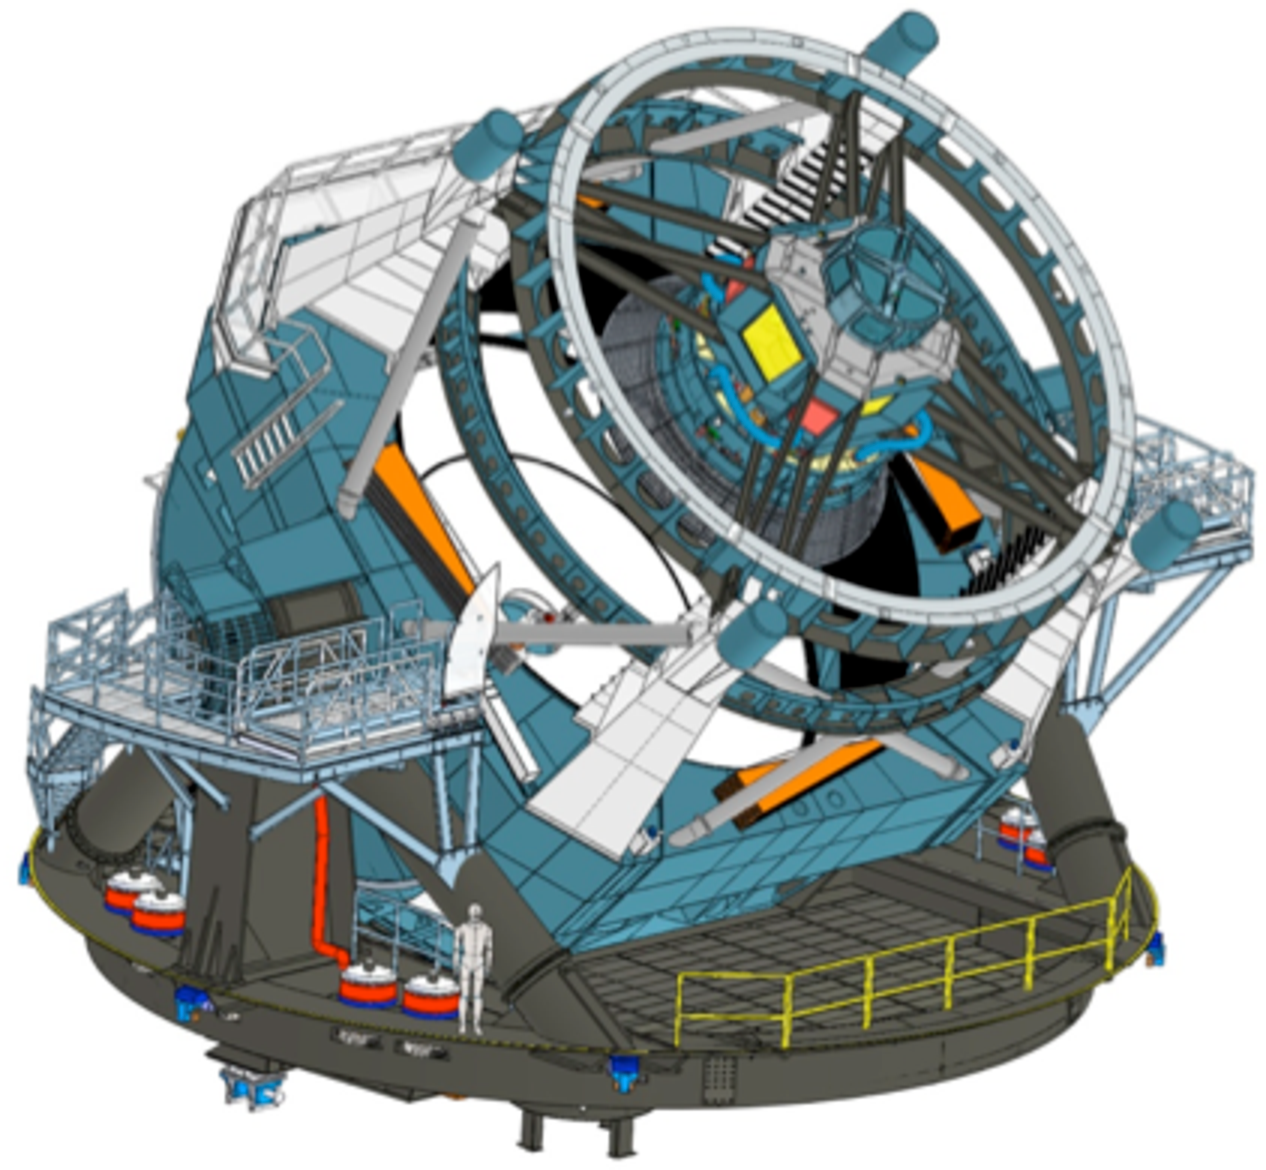
\includegraphics[width=1.0\hsize,clip]{telescopeGreen.pdf}
\vskip -0.65in
\caption{The baseline design (modified three-mirror Paul-Baker) for the 
LSST telescope.} 
\label{Fig:telescope}
\end{figure}


\begin{figure}
\vskip -1.3in
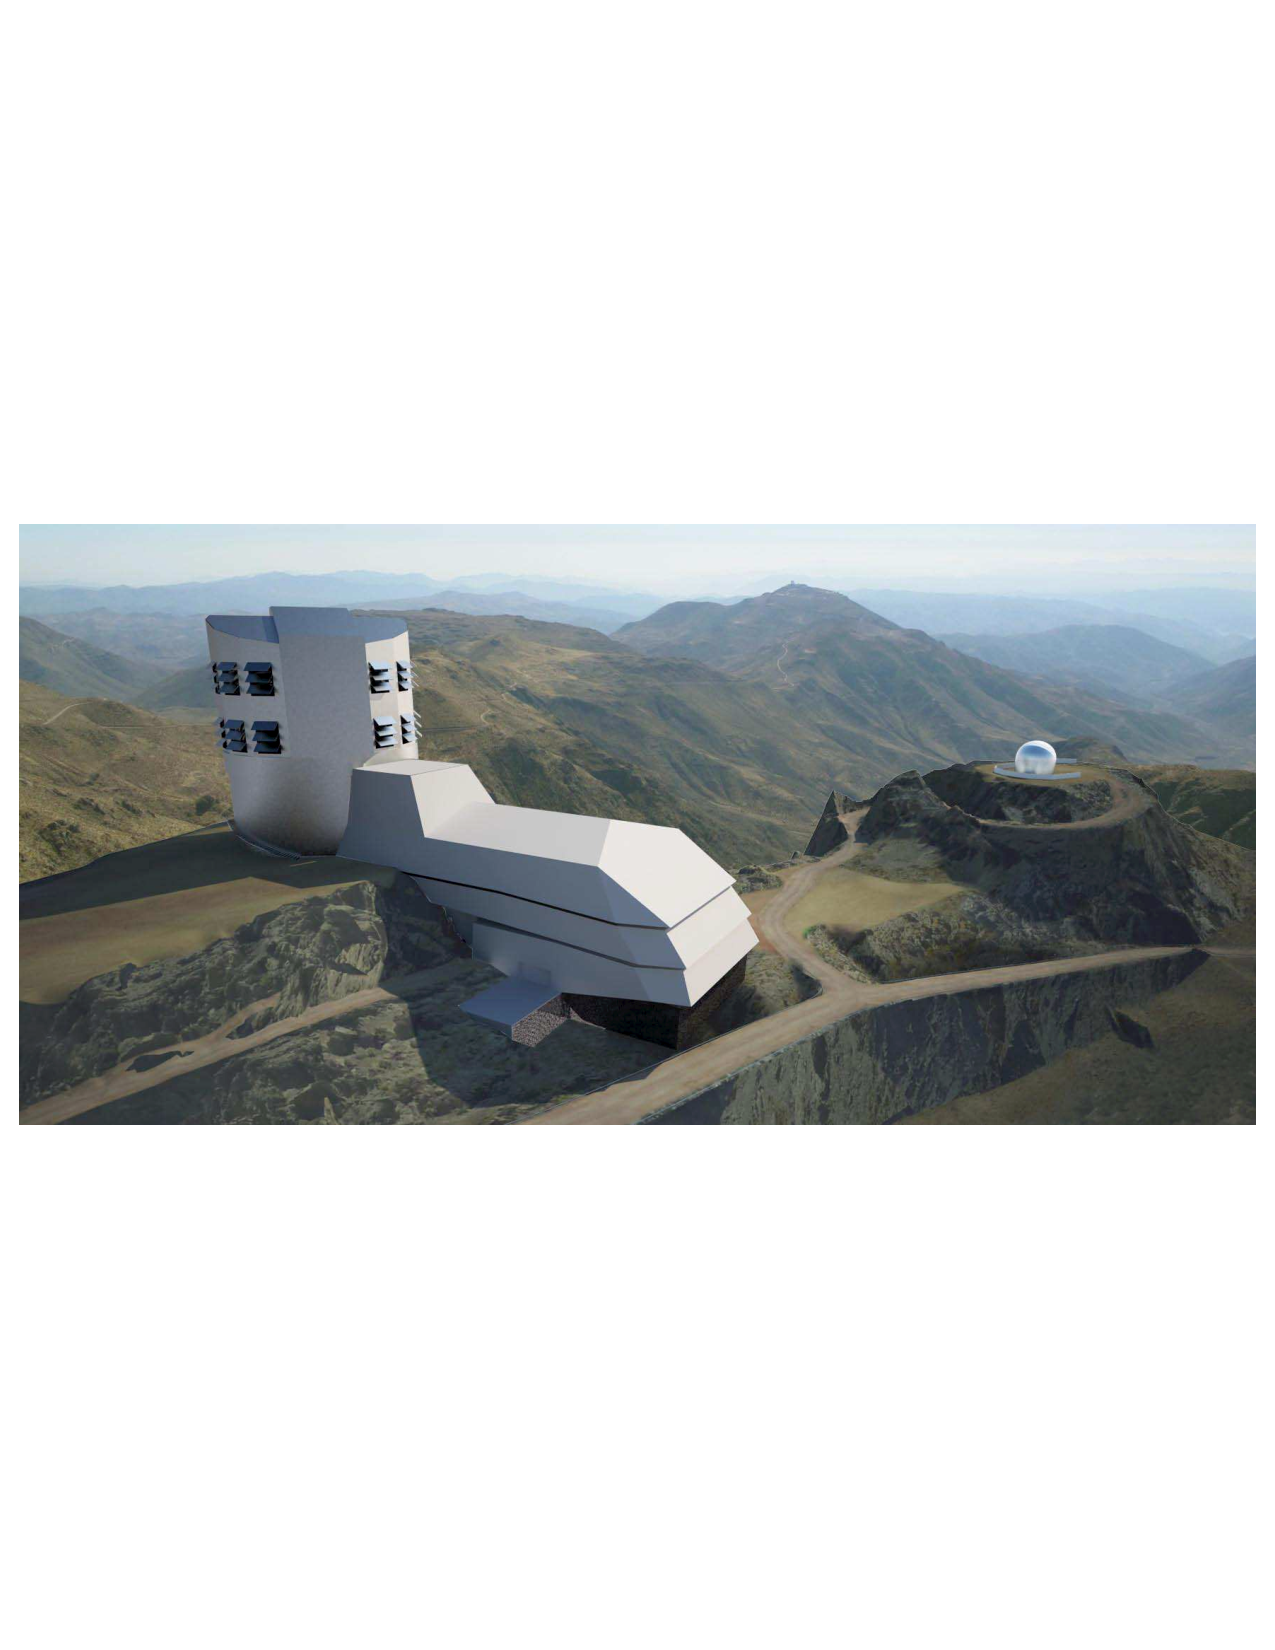
\includegraphics[width=1.0\hsize,clip]{observatoryFull.pdf}
\vskip -1.4in
\caption{The LSST Observatory: artist's rendering of the dome enclosure 
with the attached summit support building on Cerro Pach\'{o}n. The LSST calibration 
telescope is shown on an adjacent rise to the right.} 
\label{Fig:observatory}
\end{figure}



\vskip 0.2in
\subsubsection{ Camera }


\begin{figure}[t!]
\hskip -1.7in
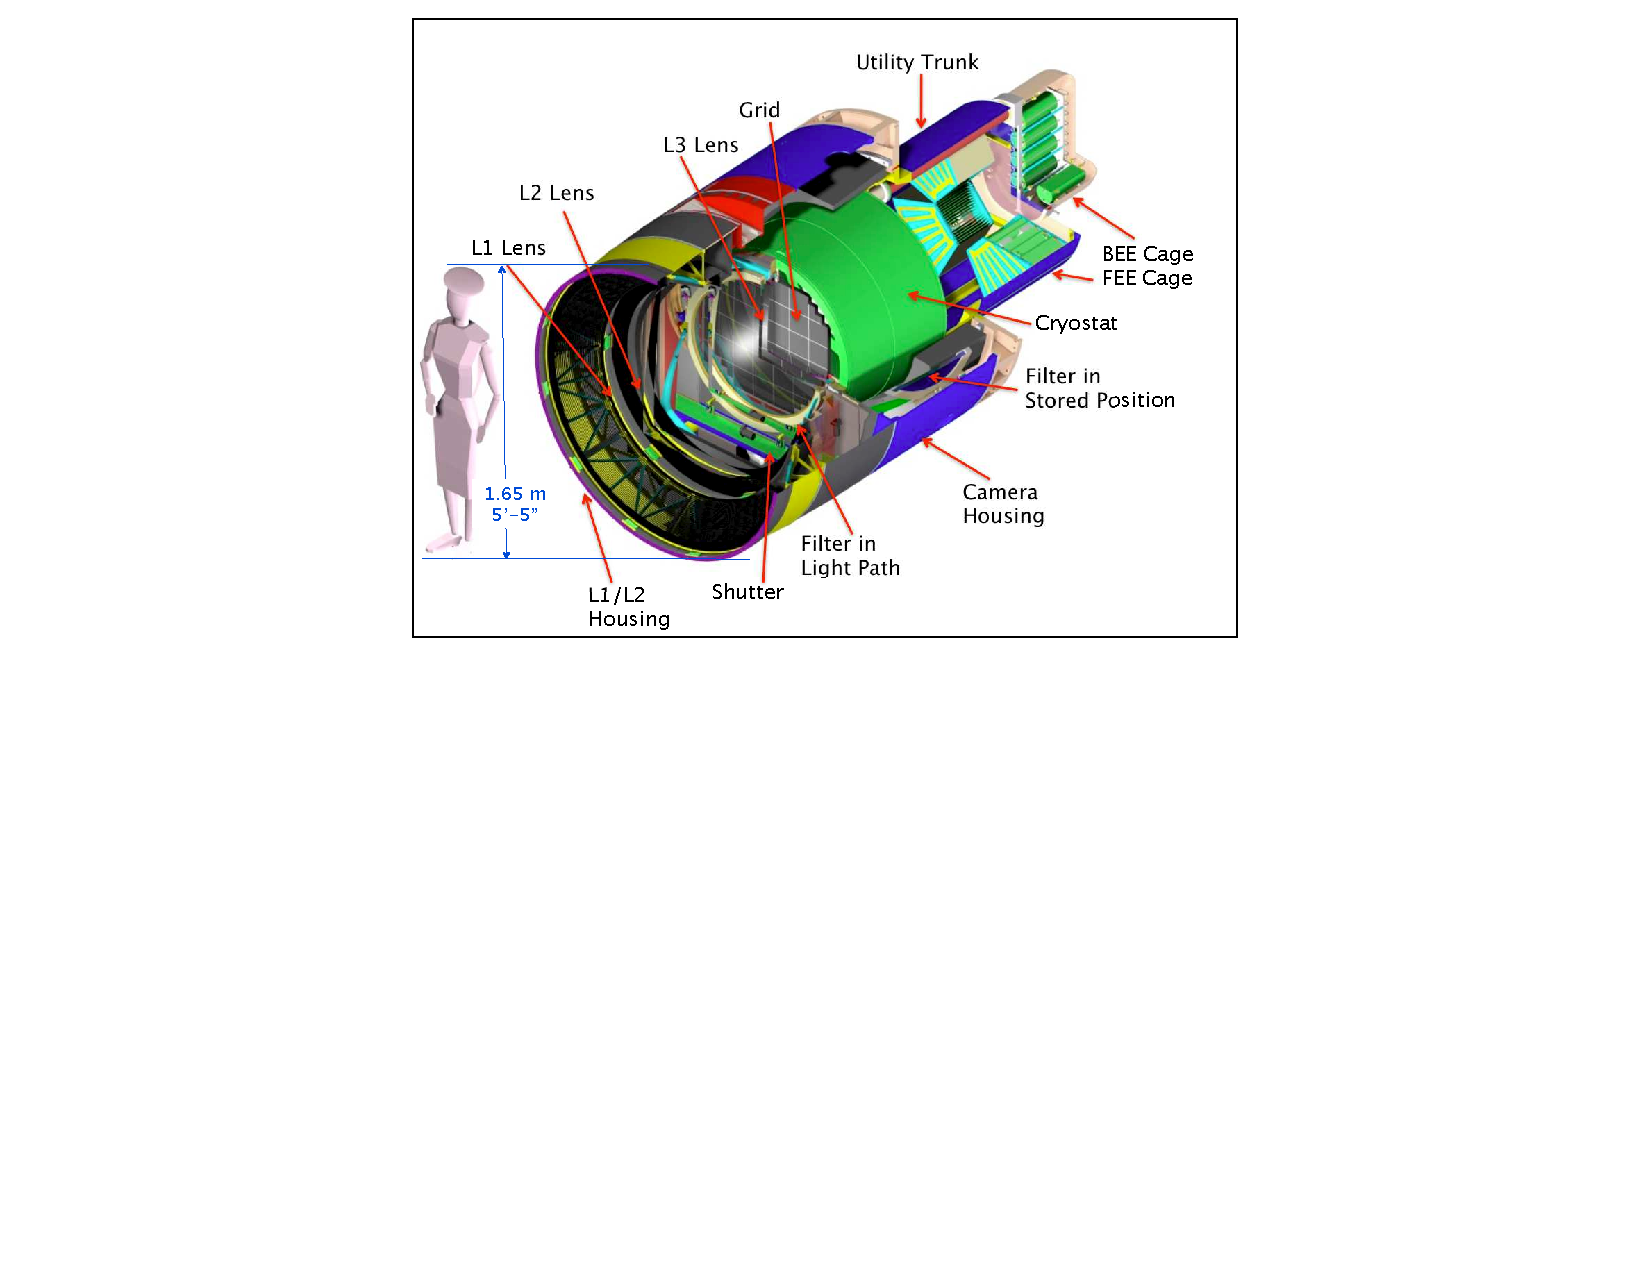
\includegraphics[width=1.55\hsize,angle=90.0,clip]{camera2009.pdf}
\vskip -2.5in
\caption{The cutaway view of LSST camera, with a person to indicate scale size. 
The camera is positioned in the middle of the telescope and will include a filter 
mechanism and shuttering capability.} 
\label{Fig:camera}
\end{figure}


\begin{figure}[ht]
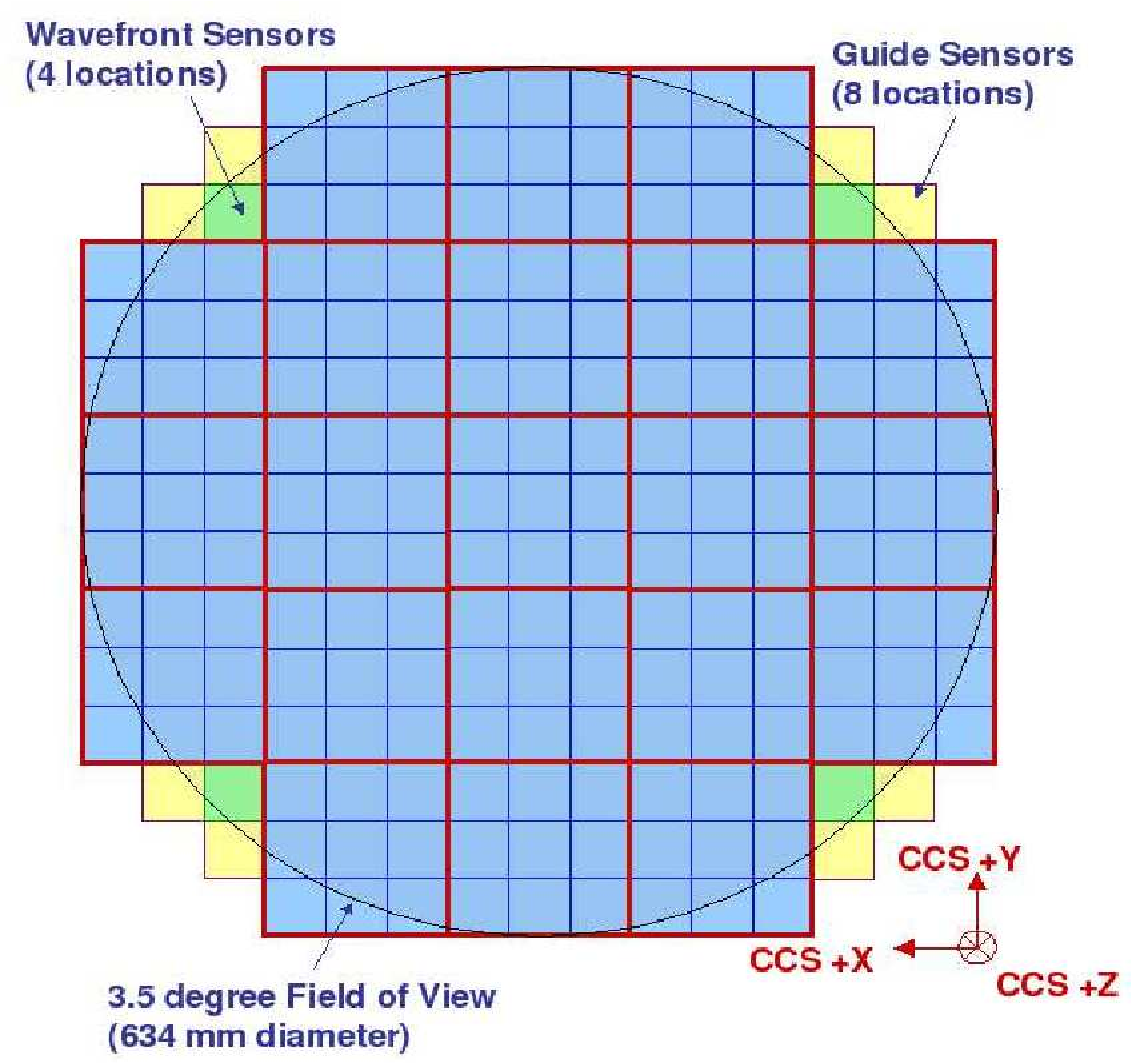
\includegraphics[width=1.0\hsize,clip]{fov.pdf}
\caption{The LSST focal plane. Each cyan square represents one
$4096\times4096$ pixel sensor. Nine sensors are assembled into a
raft; the 21 rafts are outlined in red. There are 189 science sensors, each 
with 16.8 Mpix, for a total pixel count of 3.2 Gpix.} 
\label{Fig:fov}
\end{figure}

\begin{figure}[ht]
\hskip -1.6in
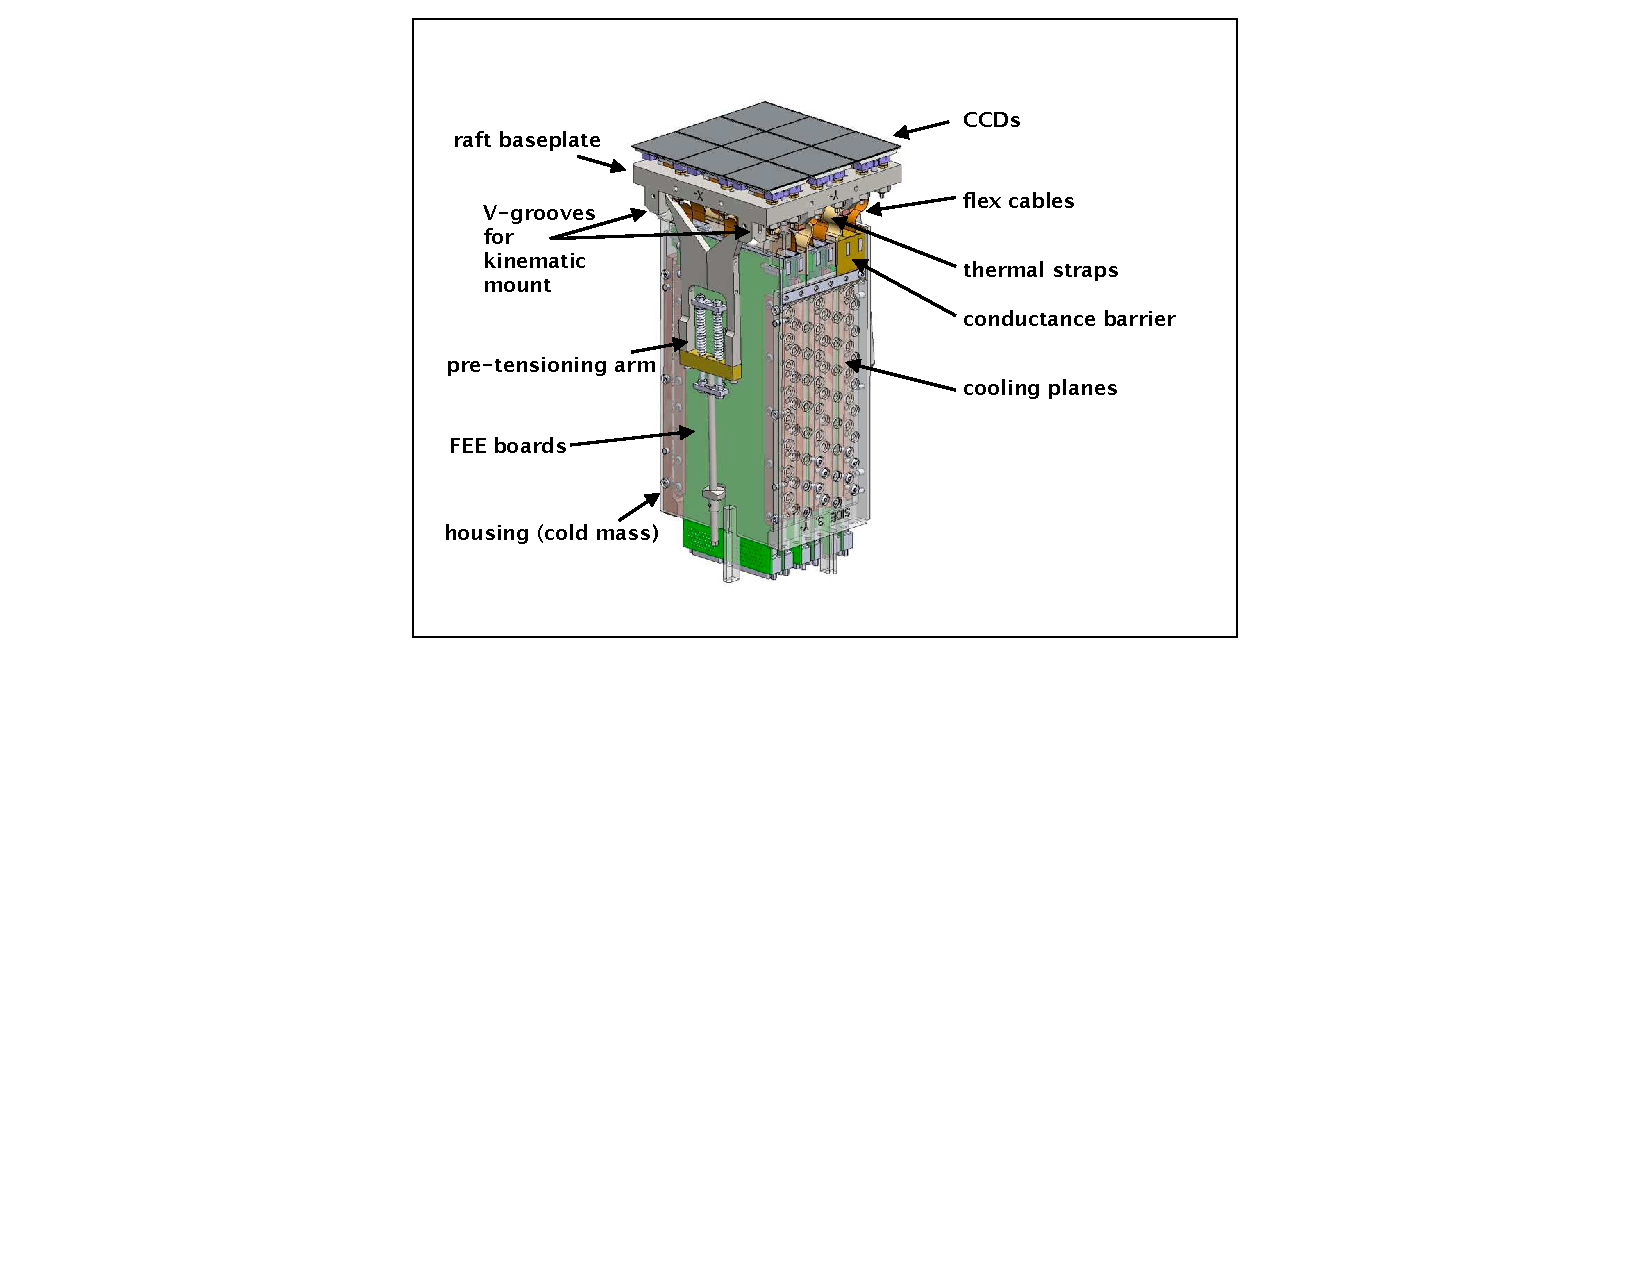
\includegraphics[width=1.5\hsize,angle=90.0,clip]{raft.pdf}
\vskip -2.5in
\caption{The LSST raft module with integrated front-end electronics
and thermal connections. Each raft (red square in Fig.~\ref{Fig:fov})
includes 9 sensors, and can be replaced.} 
\label{Fig:raft}
\end{figure}



The LSST camera provides a 3.2 Gigapixel flat focal plane array, tiled by 189
4K$\times$4K CCD science sensors with 10 $\mu$m pixels (see Figs.~\ref{Fig:camera}
and \ref{Fig:fov}). This pixel count is a direct consequence of sampling the 
9.6 deg$^2$ field-of-view (0.64m diameter) with 0.2$\times$0.2 arcsec$^2$
pixels (Nyquist sampling in the best expected seeing of $\sim$0.4 arcsec). 
The sensors are deep depleted high resistivity silicon back-illuminated devices with a highly segmented 
architecture that enables the entire array to be read in 2 seconds. 
The detectors are grouped into 3$\times$3 rafts (see Fig.~\ref{Fig:raft}); each 
contains its own dedicated front-end and back-end 
electronics boards. The rafts are mounted on a silicon carbide grid inside a 
vacuum cryostat, with an intricate thermal control system that maintains the
CCDs at an operating temperature of 180 K. The entrance window to the
cryostat is the third of the three refractive lenses in the camera. The other
two lenses are mounted in an optics structure at the front of the camera body, which 
also contains a mechanical shutter, and a carousel assembly that holds five
large optical filters. The sixth optical filter can 
replace any of the five via a procedure accomplished during daylight hours. 



\vskip 0.2in
\subsubsection{ Data Management }


The rapid cadence of the LSST observing program will produce an enormous
volume of data ($\sim$15 TB of raw imaging data per night), leading to a total database over 
the ten years of operations of 100 PB for the imaging data, and 50 PB for the catalog database. 
For comparison, the image volume in SDSS Data Release 7 is 16 TB. 
The total LSST data volume after processing will be several hundred PB.
The computing power required to process the data grows as the survey
progresses, starting at
 $\sim$100 TFlops and increasing to $\sim$400 TFlops by the end of the survey. Processing 
such a large volume of data, converting the raw images into a faithful
representation of the Universe, automated data quality assessment, and 
archiving the results in useful form for a broad community of users are
major challenges.

\begin{figure}
\vskip 0.1in
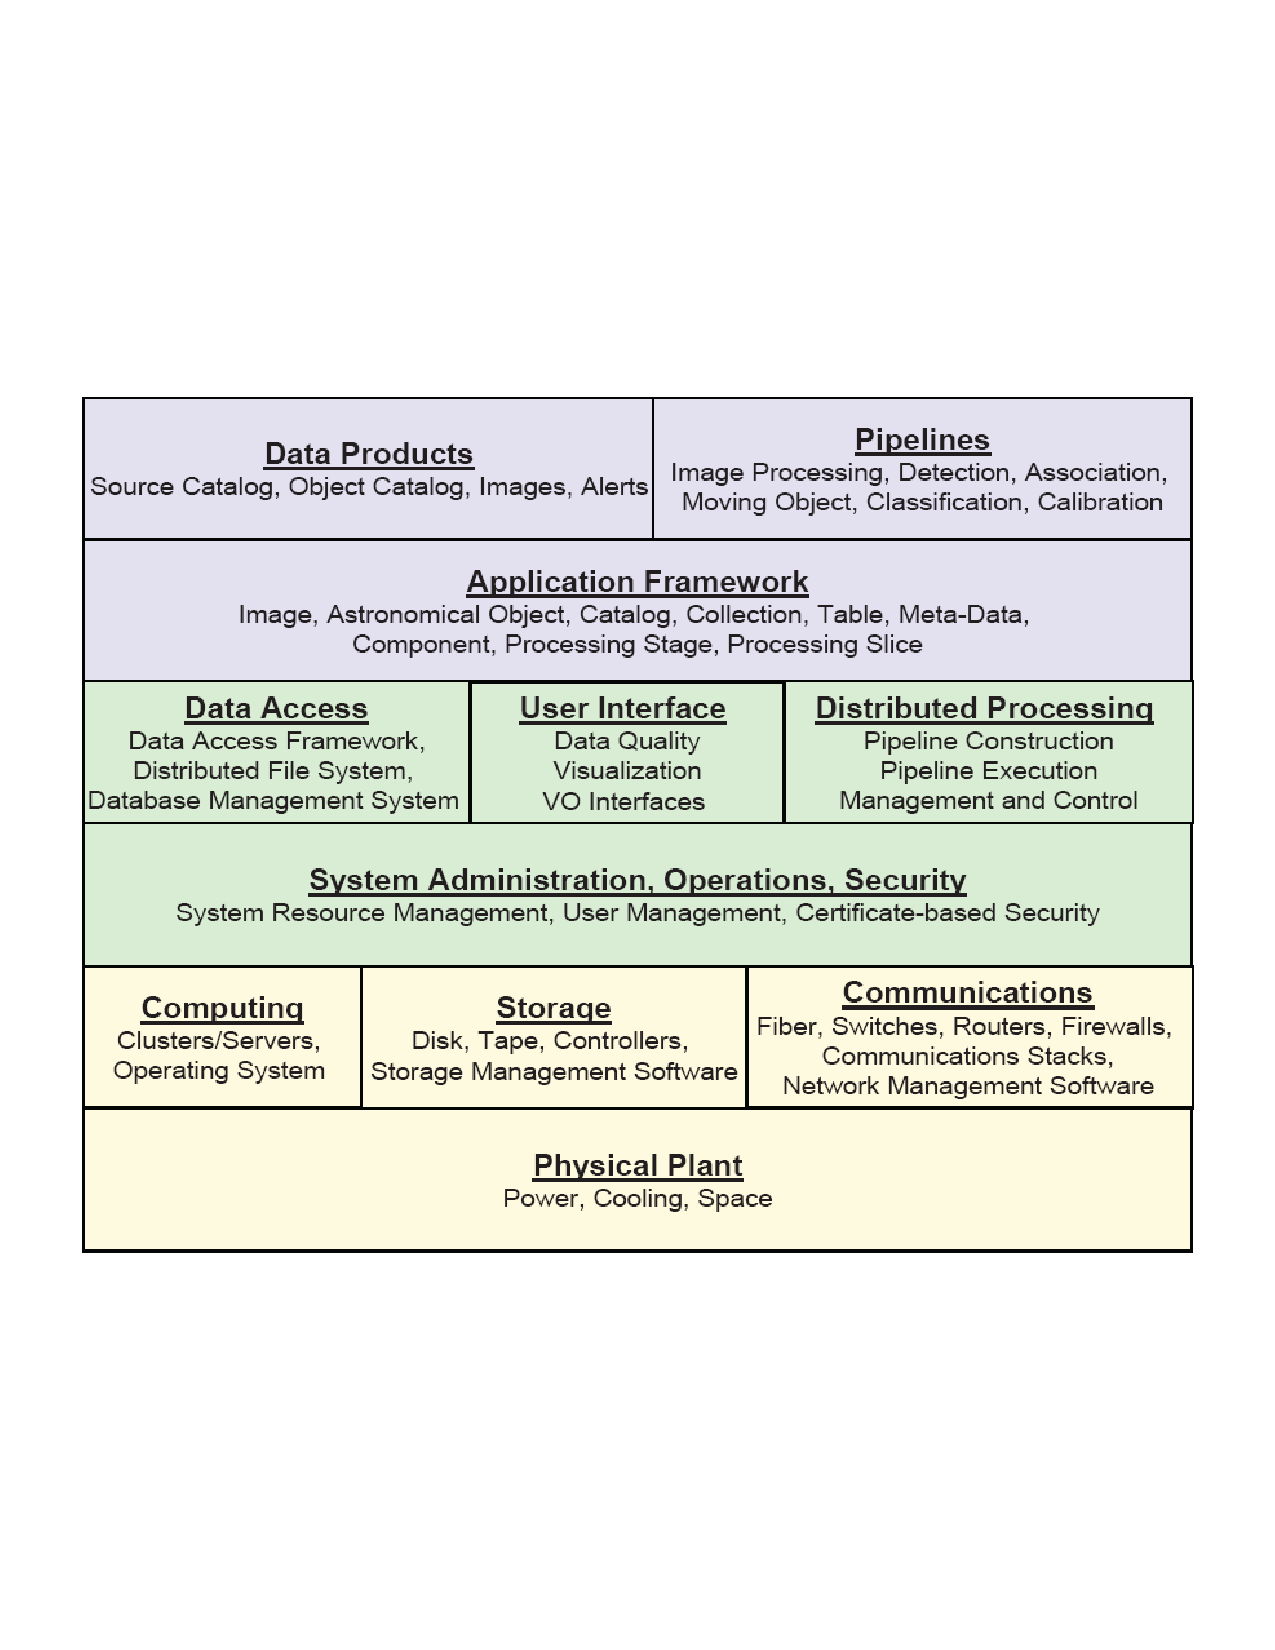
\includegraphics[width=1.0\hsize,clip]{DMsandwich.pdf}
\caption{The three-layered architecture of the data management system 
(application [purple], middleware [green], and infrastructure [yellow] layers) 
enables scalability, reliability, and evolutionary capability.} 
\label{Fig:DM1}
\end{figure}

The data management system is configured in three levels: an
infrastructure layer consisting of the computing, storage, and
networking hardware and system software; a middleware layer, which
handles distributed processing, data access, user interface, and
system operations services; and an applications layer, which includes
the data pipelines and products and the science data archives (see
Fig.~\ref{Fig:DM1}). The application layer (see Fig.~\ref{Fig:DM4})
is organized around the data products being produced.  The nightly
pipelines (see Fig.~\ref{Fig:DM5}) are based on image subtraction,
and are designed to rapidly detect interesting transient events in the
image stream and send out alerts to the community within 60 seconds of
completing the image readout.  The data release
pipelines (see Fig.~\ref{Fig:DM6}), in contrast, are intended to
produce the most completely analyzed data products of the survey, in
particular those that measure very faint objects and cover long time
scales. A new run will begin each year, processing the entire survey data
set that is available to date. The data release pipelines consume most of the
computing power of the data management system.  The calibration
products pipeline produces the wide variety of calibration data
required by the other pipelines.  All of these pipelines are
architected to make efficient use of Linux clusters with thousands of
nodes.

There will be computing facilities at the base facility in La Serena,
at a central archive facility, and at multiple data access 
centers. The data will be transported over existing high-speed optical fiber 
links from South America to the U.S. (see Fig.~\ref{Fig:DM2}).
Although the data processing center will have substantial computing power ($\sim$400 
TFlops, equal to the world's most powerful computer in 2007), the continuation of 
current trends suggests that the center will 
not even qualify for the top 500 list by the time of first light.
Hence, while LSST is making a novel use of advances in information technology, 
it is not taking the risk of pushing the expected technology to the limit.  


\begin{figure}[t!]
%\includegraphics[width=1.0\hsize,clip]{DMp1.pdf}
\hskip -0.1in
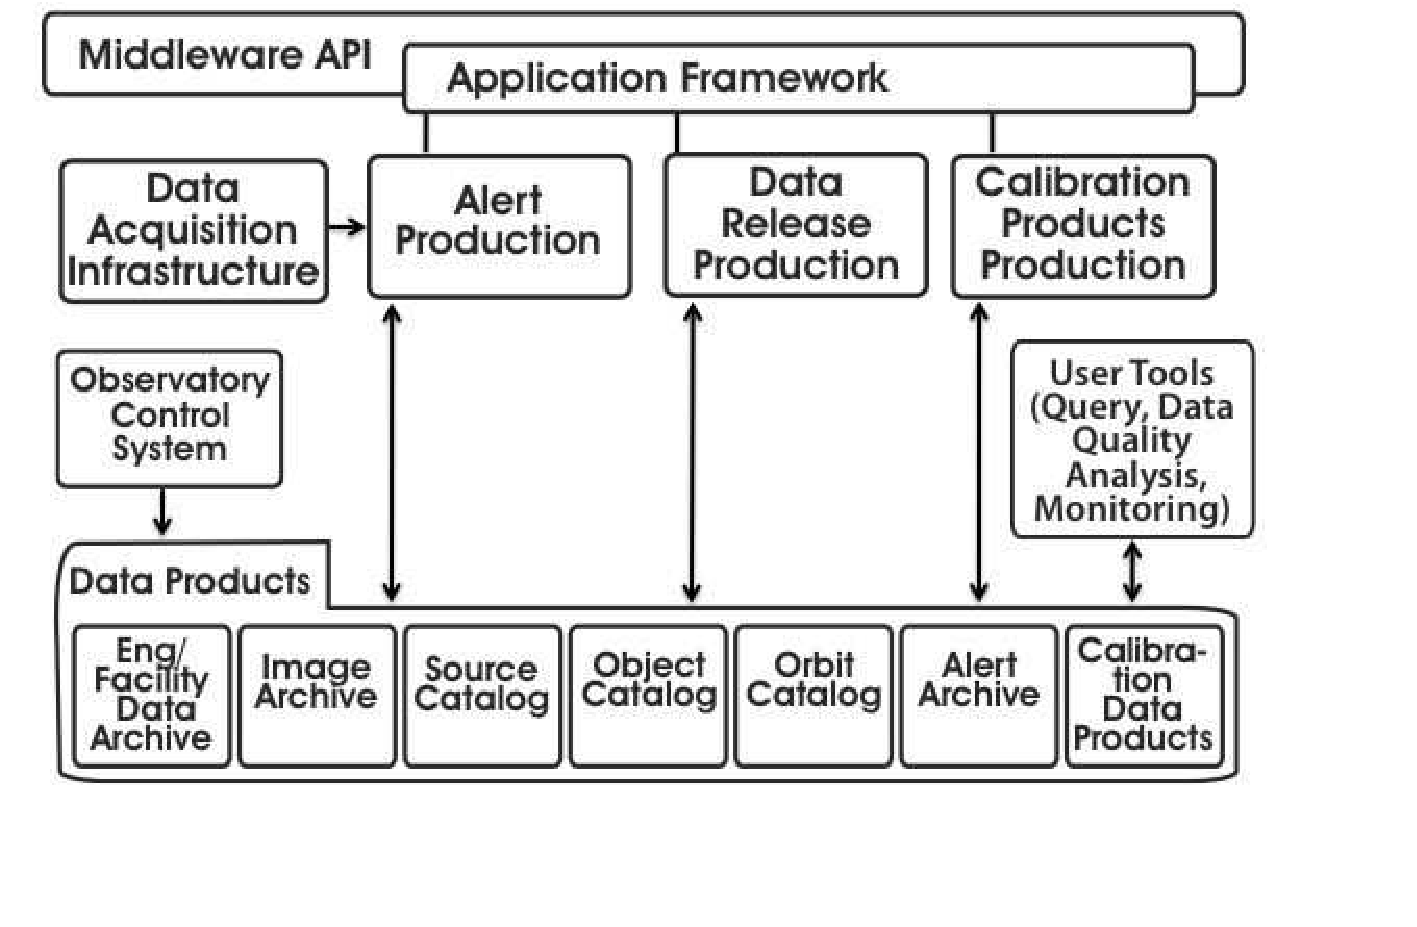
\includegraphics[width=1.15\hsize,clip]{DMp2.pdf}
%\includegraphics[width=1.0\hsize,clip]{DMfig14.pdf}
\vskip -0.3in
\caption{The application layer of the data management system. The arrows indicate
direction of the data flow. The main pipelines enable nightly processing,
calibration, and data releases.} 
\label{Fig:DM4}
\end{figure}

\begin{figure}
%\hskip -0.25in
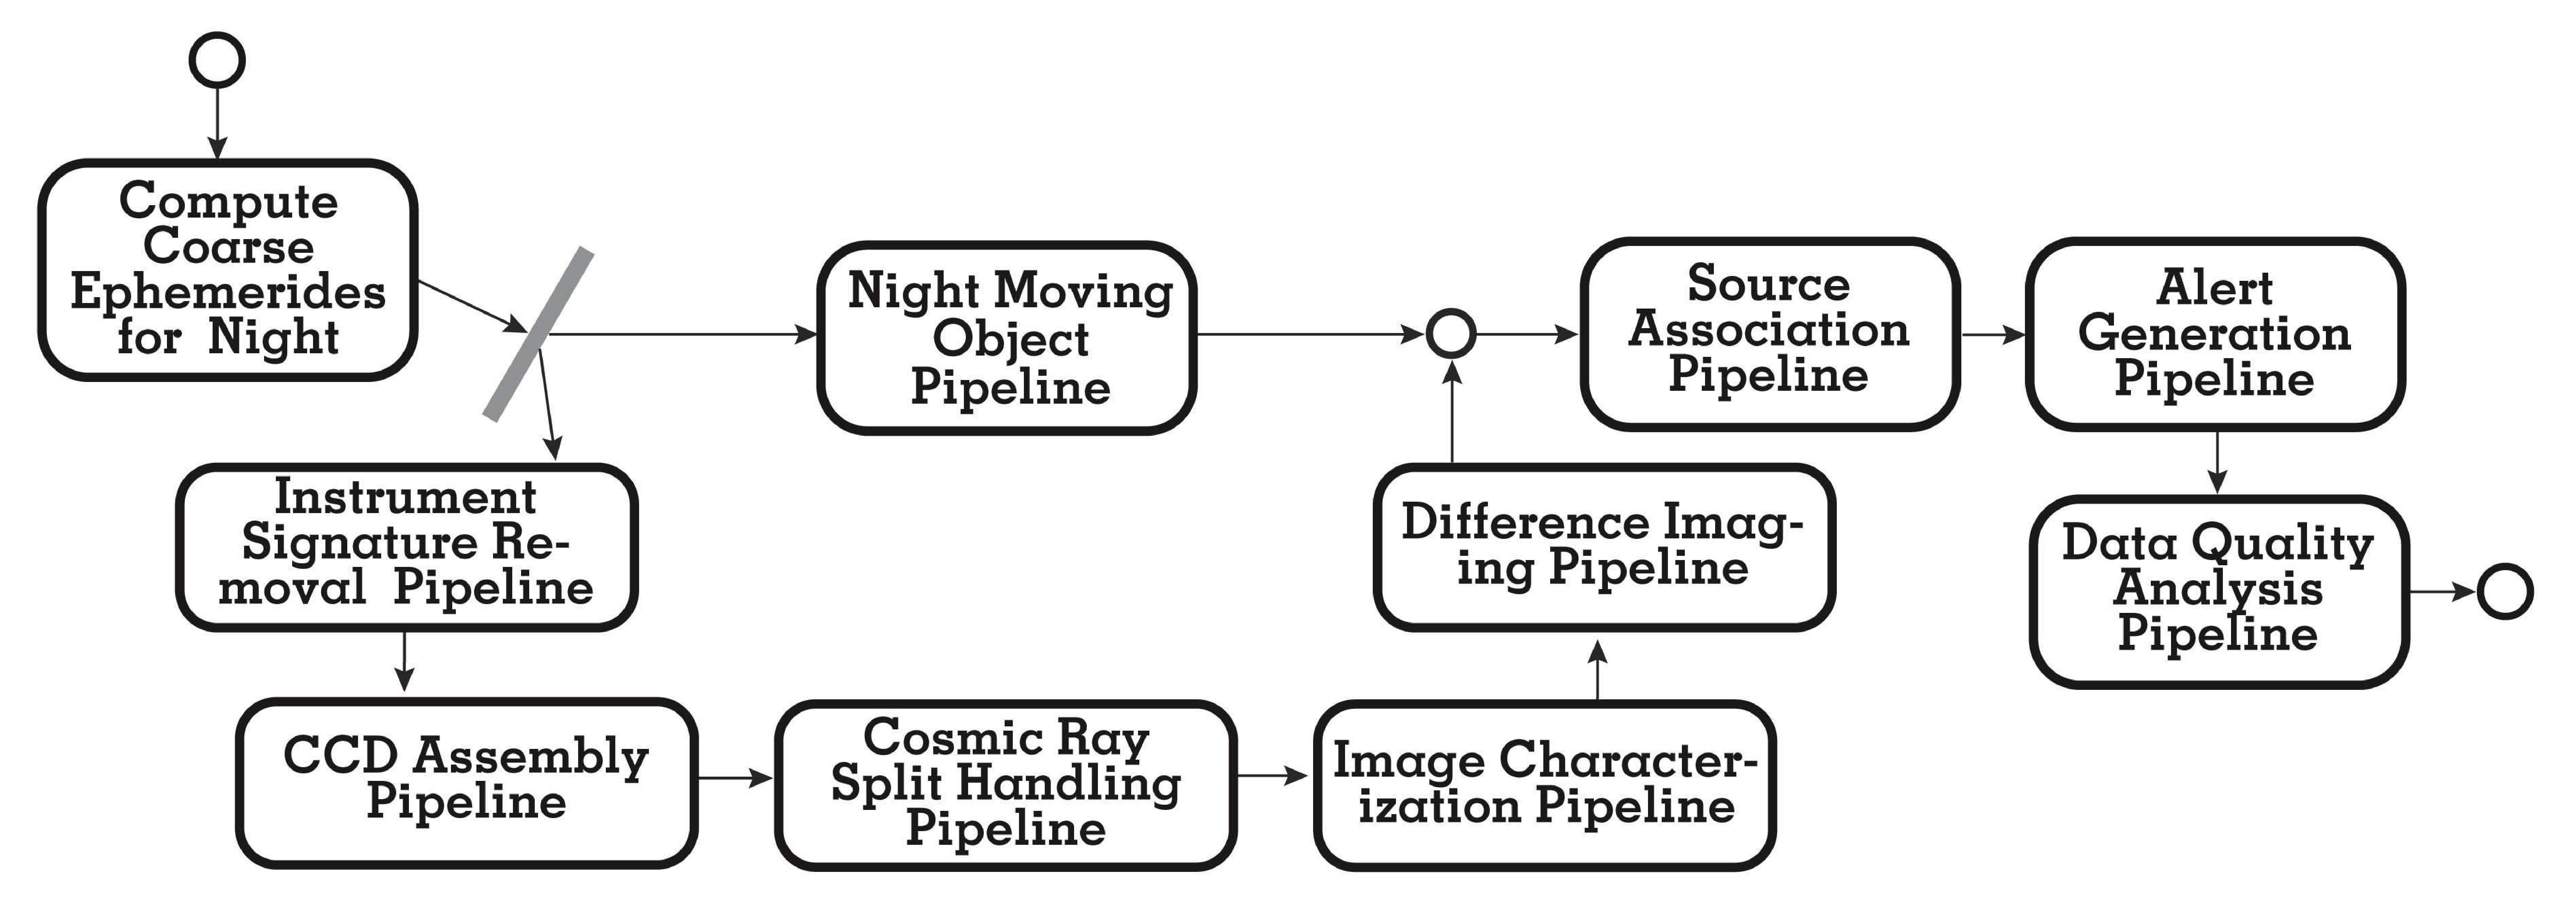
\includegraphics[width=1.0\hsize,clip]{DMp4.pdf}
%\includegraphics[width=1.0\hsize,clip]{DMfig14.pdf}
%\vskip -0.4in
\caption{The structure of nightly (``alert generation'') pipelines. 
Their main task is to compare new data to the previously accumulated data and search for 
transient, variable and moving objects.} 
\label{Fig:DM5}
\end{figure}

\begin{figure*}[t!]
\hskip 0.3in
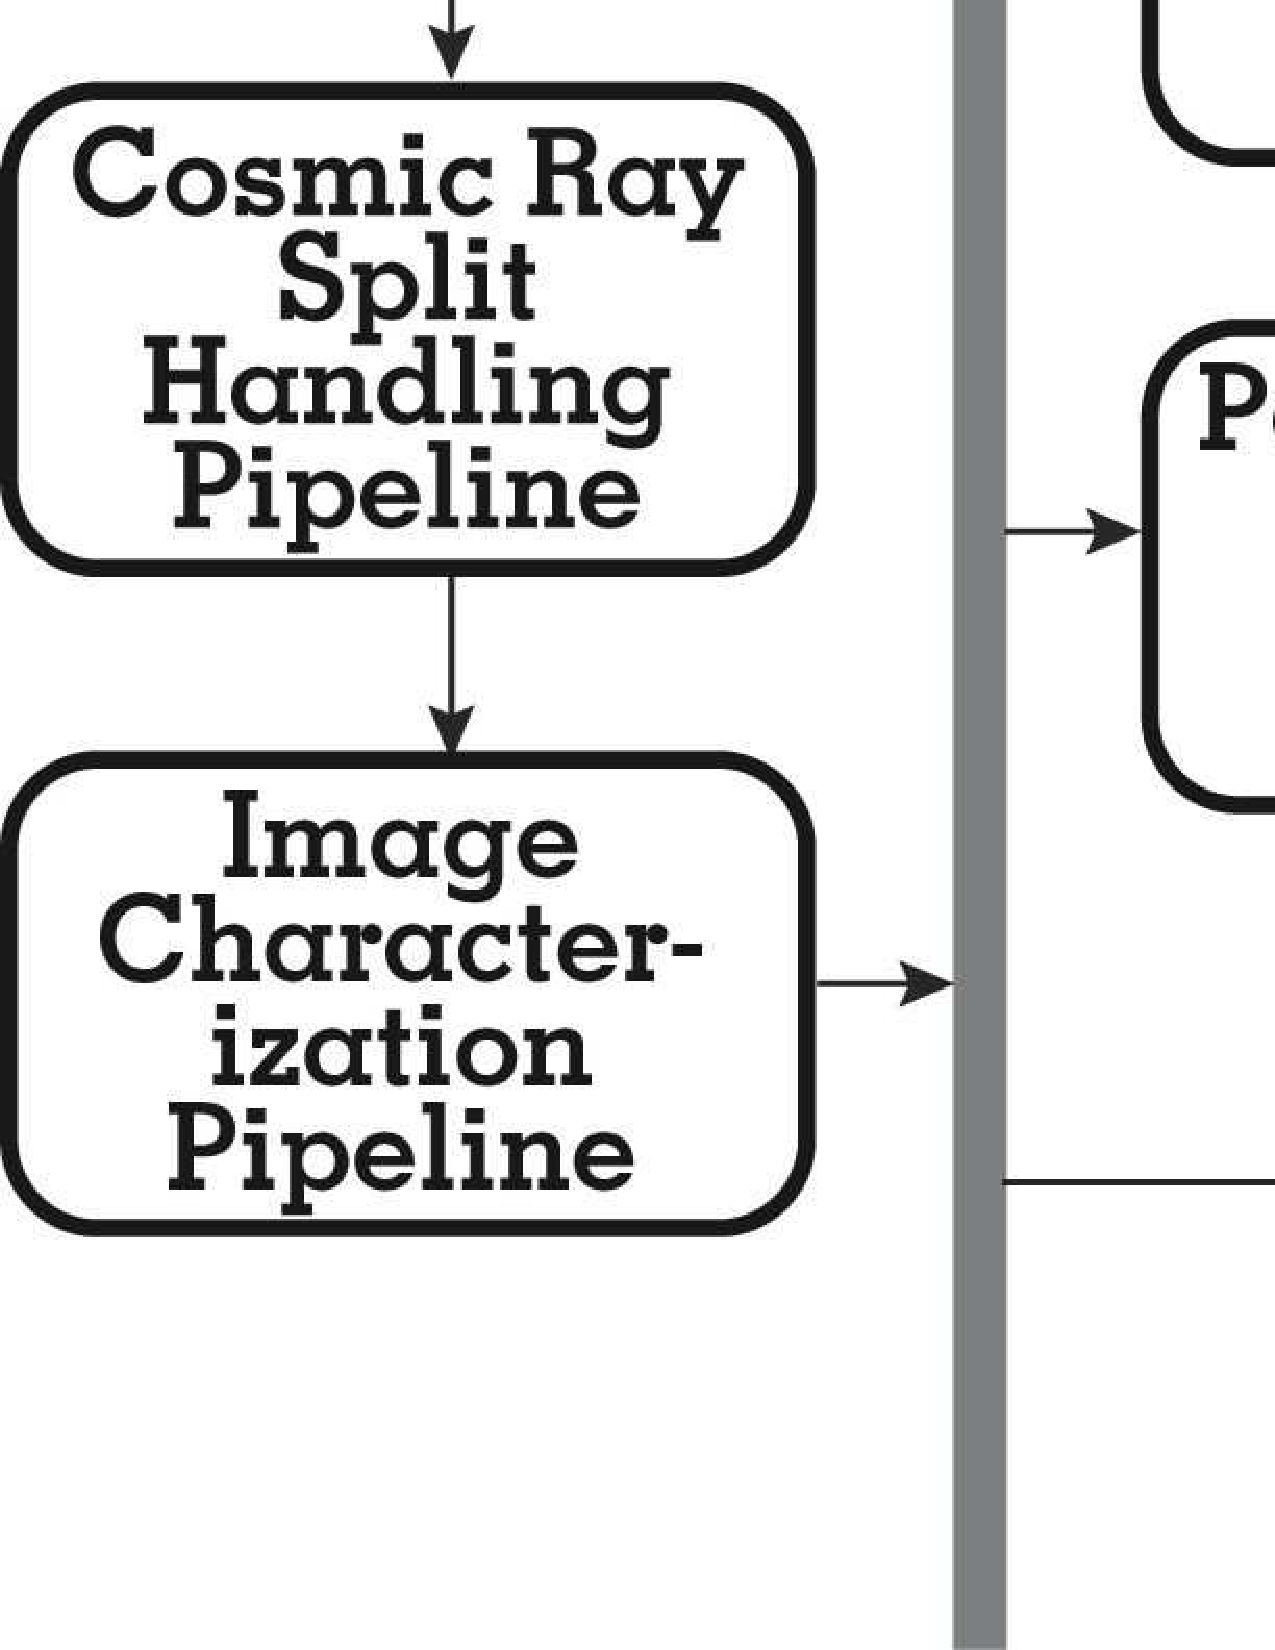
\includegraphics[width=0.92\hsize,clip]{DMp3.pdf}
\caption{The structure of data release pipelines.
These pipelines are intended to produce the most completely analyzed data products 
of the survey, and will consume most of the computing power of the data management 
system.} 
\label{Fig:DM6}
\end{figure*}


\begin{figure*}
\hskip 0.5in
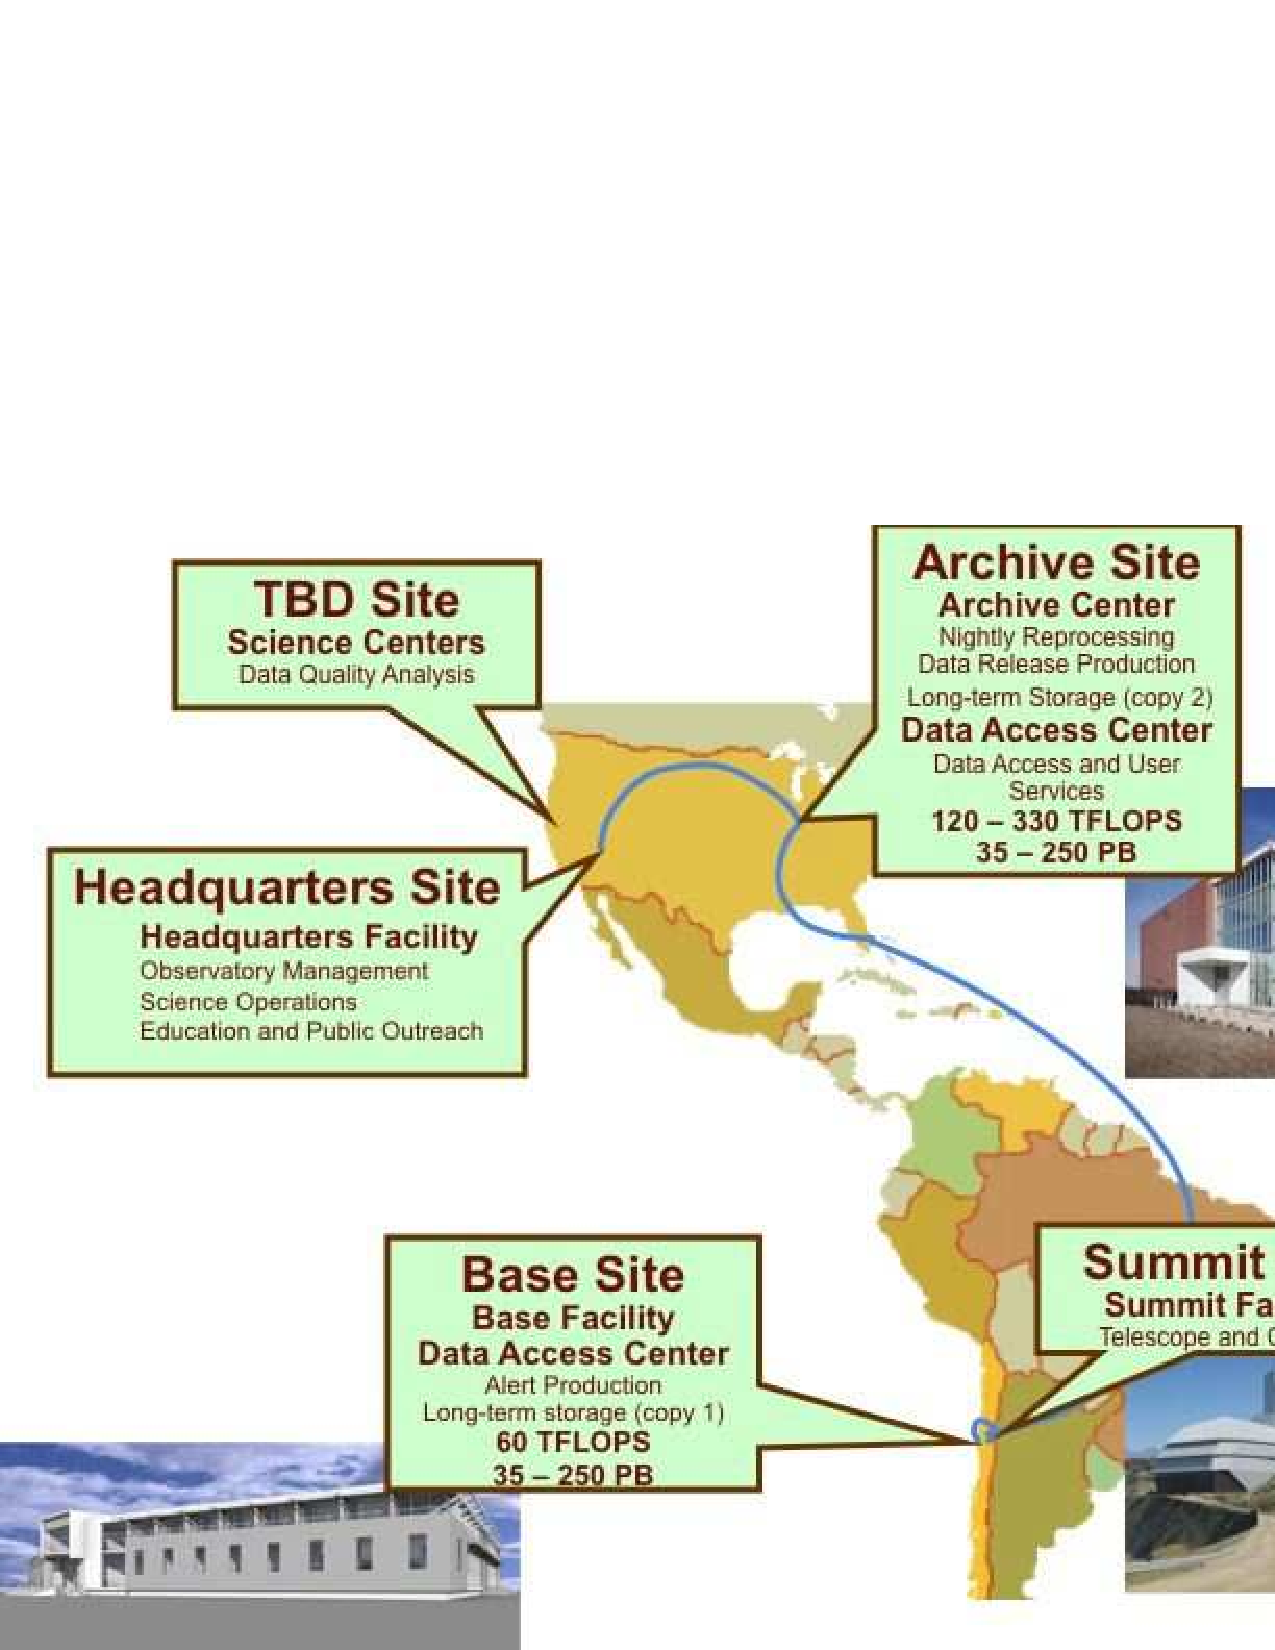
\includegraphics[width=0.9\hsize,clip]{DMX2.pdf}
\caption{The LSST data flow from the mountain summit/base facility in
Chile to the data access center and archive centers in the U.S.} 
\label{Fig:DM2}
\end{figure*}



\B{
\vskip 0.4in
\subsection{Simulating the LSST System}


Throughout its design, construction and commissioning, the LSST needs
to be able demonstrate that it can achieve the requirements laid out
in the Science Requirements Documents (SRD) given its design and
as-delivered components, that the system can be calibrated to the
required level of fidelity, that the data management software can
extract the appropriate astrophysical signals, and that this can be
achieved with sufficient efficiency such that the telescope can
complete its primary objectives within the ten years of its duration
(including surveying 18,000 sq degrees of the sky, and completing the
Deep Drilling Fields, \citealt{jones2013}).


Realizing these objectives requires that the project can characterize
the performance of the LSST including the performance of the
opto-mechanical systems, the response of the detectors and their
electronics, and the capabilities of the analysis software. A
simulation framework provides such a capability; delivering a virtual
prototype LSST against which design decisions, optimizations
(including descoping), and trade studies can be evaluated (Connolly,
et al. 2010).


The framework underlying the LSST simulations is designed to be
extensible and scalable (i.e. capable of being run on a single
processor or across many-thousand core compute clusters). It comprises
four primary components: a simulation of the survey scheduler,
databases of simulated astrophysical catalogs of stars, galaxies,
quasars and solar system objects, a system for generating observations
based on the pointing of the telescope and a series of algorithms for
simulating LSST images. Computationally intensive routines are written
in $C/C^{++}$ with the overall framework and database interactions
using $Python$.  The purpose of this design is to enable the
generation of a wide range of data products for use by the
collaboration; from all-sky catalogs used in simulations of the LSST
calibration pipeline, to studies of the impact of survey cadence on
recovering variability, to simulated images of a single LSST focal
plane.


\subsection{ The LSST Operations Simulator }

The LSST Operations Simulator was developed to enable a 
detailed quantitative analysis of the various science tradeoffs described in 
this paper. It contains detailed models of site conditions, hardware and
software performance, and an algorithm for scheduling observations which will, 
eventually, drive the largely robotic observatory. 
Observing conditions include a model for seeing derived from an extensive body
of on-site MASS/DIMM (Multi-Aperture Scintillation Sensor and Differential
Image Motion Monitor) measurements obtained during site selection and
characterization (see Fig.~\ref{Fig:seeing}). It not only reproduces the 
observed seeing distribution, but includes 
the auto-correlation spectrum of seeing with time over intervals from minutes 
to seasons. Weather data are taken from ten years of hourly measurements at
nearby Cerro Tololo. The time history of site conditions is important if the 
simulation is to faithfully reproduce a sequence of observations. Thus, for
example, the simulator correctly represents the variation of limiting
magnitude between pairs of observations used to detect NEOs and the
correlation between, for example, seasonal weather patterns and observing
conditions at any given point on the sky. The signal-to-noise ratio of each 
observation is determined using a sky background model which includes the dark
sky brightness in each filter, the effects of seeing and atmospheric
transparency, and a detailed model for scattered light from the moon and/or 
twilight at each observation. The time taken to move from one observation to
the next is given by a detailed model of the camera, telescope, and dome. It 
includes such effects as the acceleration/deceleration profiles employed in 
moving in altitude, azimuth, camera rotator, dome azimuth, and wind/stray
light screen altitude, the time taken to damp vibrations excited by each slew, 
cable wrap, time taken for active optics lock and correction as a function of 
slew distance, filter change, and focal plane readout. The time required for
observatory maintenance is also simulated. 

Observations are scheduled by a ranking algorithm. After a given exposure, all 
possible next observations are assigned a score which depends upon their locations, times,
and filters according to a set of scientific requirements which can vary with 
time and location. For example, if an ecliptic field has been observed in the
$r$ band, the score for another $r$-band observation of the same field will 
initially be quite low, but it will rise in time to peak about an hour after
the first observation, and decline thereafter. This results in these
observations being acquired as pairs roughly an hour apart, which enables
efficient association of NEO detections. To ensure uniform 
sky coverage, fields with fewer previous observations will be scored more
highly than those which have already been observed more frequently.
 
Once all possible next observations have been scored for scientific
priority, their scores are modified according to observing conditions
(e.g., seeing, airmass, and sky brightness) and to criteria such as
low slew time to move from the current position, time required to
change filters, etc. The highest-ranked observation is then performed,
and the cycle repeats. The result of a simulator run is a detailed
history of which locations on the sky were observed when, in what
filter, and with what sky background, seeing and other observing
conditions.  It takes a few days to produce a decade-long simulation
using an average PC.

\subsubsection{Catalog Generation}

The simulated astronomical catalogs are stored in an SQL
database. This base catalog is queried using sequences of observations
derived from the Operations Simulator. Each simulated
pointing provides a position and time of the observation together with
the appropriate sky conditions (e.g. seeing, moon phase and angle, sky
brightness and sky transparency). Positions of sources are propagated
to the time of observation (including proper motion for stars and
orbits for Solar System sources). Magnitudes and source counts are
derived using the atmospheric and filter response functions
appropriate for the airmass of the observation and after applying
corrections for source variability.  The resulting catalogs are then
formatted for either output to users, or fed into an image
simulator. Images are generated by ray-tracing individual photons
through the atmosphere, telescope and camera systems. Photons are
drawn from the spectral energy distributions that define the simulated
sources and ray-traced through the atmosphere and optical system
before conversion to electrons by simulating the camera physics.
Images are read out using a simulation of the camera electronics and
amplifier layout and formatted for ingestion into the LSST data
management system. All observing conditions, defined by the Operations
Simulator, are propagated through the catalog and image generation to
preserve fidelity and consistency between the derived catalogs and
images.
 
The current version of the LSST simulation framework incorporates
galaxies derived from an N-body simulation of a $\Lambda$-CDM
cosmology, quasars/AGNs, stars that match the observed stellar
distributions within our Galaxy, asteroids generated from simulations
of our Solar System, and a 3-D model for Galactic extinction.  Stellar
sources are based on the Galactic structure models of Juri\'{c} et
al. (2008) and include thin-disk, thick-disk, and halo star
components. The distribution and colors of the stars match those
observed by SDSS. Each star in the simulation is matched to a template
spectral energy distribution (SED). Kurucz (1993) model spectra are
used to represent main-sequence F, G, and K stars as well as RGB
stars, blue horizontal branch stars, and RR Lyrae variables.  SEDs for
white dwarf stars are taken from Bergeron et al. (1995).  SEDs for M,
L, and T dwarfs are generated from a combination of spectral models
and by stacking spectra from the SDSS (e.g., Cushing et al. 2005,
Bochanski et al. 2007, Burrows et al. 2006, Petterson \& Hawley 1989,
Kowalski et al. 2010). The adopted metallicity for each star is based
on a model from Ivezi\'{c} et al. (2008a), and proper motions are
based on the kinematic model of Bond et al. (2010).  Light curve
templates are randomly assigned to a subset of the stellar population
so that variability may also be simulated. For Galactic reddening, a
value of $E(B-V)$ is assigned to each star using the three-dimensional
Galactic model of Amores \& Lepine (2005). To provide consistency with
extragalactic observations the dust model in the Milky Way is
re-normalized to match the Schlegel et al. (1998) dust maps at a
fiducial distance of 100 kpc.

Galaxy catalogs are derived from the Millennium simulations of de
Lucia et al. (2006).  These models extend the dark matter N-body
simulations to include gas cooling, star formation, supernovae and
AGN, and are designed to reproduce the observed colors, luminosities,
and clustering of galaxies as a function of redshift. To generate the
LSST simulated catalogs, a light-cone, covering redshifts $0<z<6$, was
constructed from 58 500h$^{-1}$Mpc simulation snapshots. This
light-cone extends to a depth of approximately $r=28$ and covers a
4.5$^\circ$$\times$4.5$^\circ$ footprint on the sky. Replicating this
catalog across the sky simulates the full LSST footprint. As with the
stellar catalog, an SED is fit to the colors of each source using
Bruzual \& Charlot (2003) spectral synthesis models. These fits are
undertaken separately for the bulge and disk components and, for the
disk, include inclination dependent reddening. Morphologies are
modeled using two Sersic profiles. The bulge-to-disk ratio and disk
scale lengths are taken from de Lucia et al. (2006). Half-light radii
for bulges are estimated using the empirical absolute-magnitude
vs. half-light radius relation given by Gonzalez et
al. (2009). Comparisons between the redshift and number-magnitude
distributions of the simulated catalogs with those derived from deep
imaging and spectroscopic surveys showed that the de Lucia et
al. models under-predict the density of sources at faint magnitudes
and high redshifts. To correct for these effects, sources are cloned
in magnitude and redshift space until their densities reflect the
average observed properties.

Quasar/AGN catalogs are generated using the Bongiorno et al. (2007)
luminosity function for $M_B < -15$, and over an area of 100
deg$^2$. Their observed SEDs are generated using a composite
rest-frame spectrum derived from SDSS data by Vanden Berk et
al. (2001). The host galaxy is selected to have the closest match to
the preferred stellar mass and color at the AGN's redshift, following
the results from Xue et al. (2010).  Each galaxy hosts at most one
AGN, and no explicit distinction is made between fainter AGN and
''quasars" that dramatically outshine their host galaxies. The light
curve for each AGN is generated using a damped random walk model and
prescriptions given by MacLeod et al. (2010).

Asteroids are simulated using the Solar System models of Grav et
al. (2007). They include: Near Earth Objects (NEOs), Main Belt
Asteroids, the Trojans of Mars, Jupiter, Saturn, Uranus, and Neptune,
Trans Neptunian Objects, and Centaurs. Spectral energy distributions
are assigned using the C and S type asteroids of DeMeo et
al. (2009). Positions for the 11 million asteroids in the simulation
are stored within the base catalog (sampled once per night for the ten
year duration of the LSST survey). Querying the base catalog returns
all sources within a given LSST pointing for which we generate
accurate ephemerides using the $PyOrb$ software package (Granvik et
al. 2009). With typically 8000 sources per LSST field of view, this
procedure was developed to decrease the computational resources
required to simulate asteroid ephemerides.



\subsubsection{Image Simulations}

The framework described above provides a parametrized view of the sky
above the atmosphere. To generate images, photons are drawn from the
spectral energy distribution of each source (scaled to the appropriate
flux density based on the apparent magnitude of a source and
accounting for the spatial distribution of light for extended
sources). Each photon is ray-traced through the atmosphere, telescope
and camera to generate a CCD image. The atmosphere is modeled using a
Taylor frozen screen approximation (with the atmosphere described by
six layers). The density fluctuations within these screens are
described by a Kolmogorov spectrum with an outer scale (typically 10m
to 200m). All screens move during an exposure with velocities derived
from NOAA measurements of the wind velocities above the LSST site in
Chile.  Typical velocities are on the order of 20 m s$^{-1}$, and are
found to have a seasonable dependence that is modeled when generating
the screens. Each photon's trajectory is altered due to refraction as
it passes through each screen.

After the atmospheric refraction, photons are reflected and refracted
by the optical surfaces within the telescope and camera. The mirrors
and lenses are simulated using geometric optics techniques in a fast
ray-tracing algorithm and all optical surfaces include a spectrum of
perturbations based on design tolerances. Each optic moves according
to its six degrees of freedom within tolerances specified by the LSST
system. Fast techniques for finding intercepts on the aspheric surface
and altering the trajectory of a photon by reflection or
wavelength-dependent refraction have been implemented to optimize the
efficiency of the simulated images. Wavelength and angle-dependent
transmission functions are incorporated within each of these
techniques, including simulation of the telescope spider.

Ray tracing of the photons continues into the silicon of the
detector. The conversion probability, refraction as a function of
wavelength and temperature, and charge diffusion within the silicon
are modeled for all photons. Photons are pixelated and the readout
process simulated including blooming, charge saturation, charge
transfer inefficiency, gain and offsets, hot pixels and columns, and
QE variations. The sky background is added as a post-processing step,
and includes Rayleigh scattering of the moon's light, based on SEDs
for the full moon and the dark sky. The background is vignetted
according to the results of ray-trace simulations.

The simulator generates $\sim$300,000 photons per second on an average
workstation. To produce simulated data corresponding to a night of
regular LSST operations requires approximately 0.5-1 million CPU hours
and, therefore, necessitates the use of large compute clusters.  An
example of a simulated image is shown in Fig.~\ref{Fig:ImSimExample}.
}

\begin{figure*}
\vskip -1in
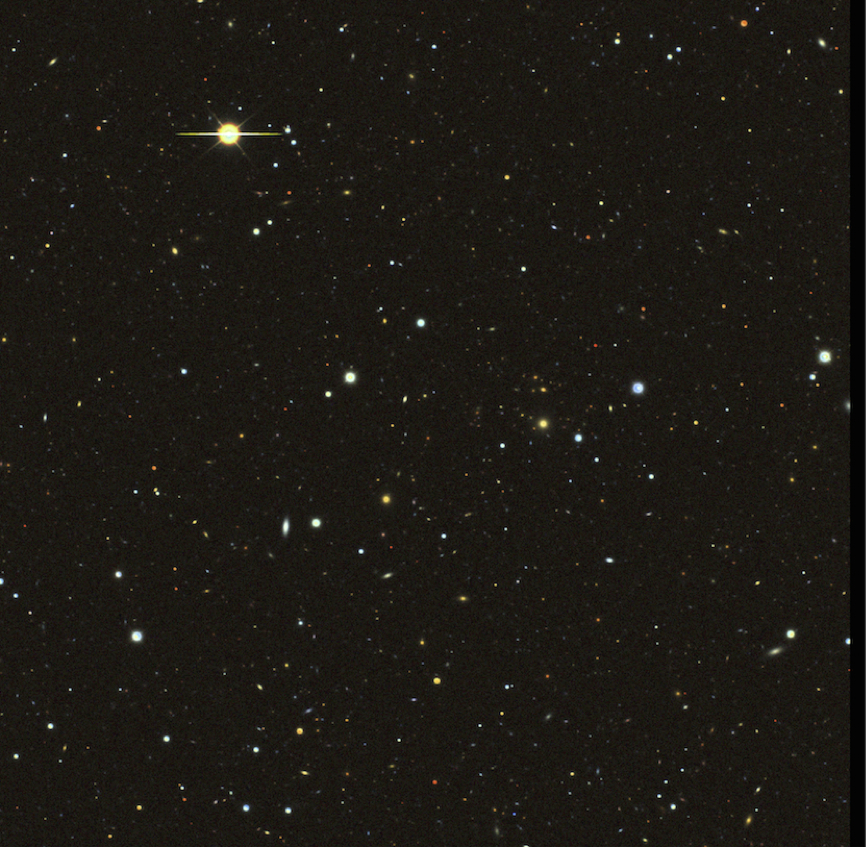
\includegraphics[width=1.0\hsize,clip]{chip2014.png}
\vskip -1in
\caption{ A simulated image of a single LSST CCD (covering a
  $13.3\times13.3$ arcmin$^2$ region of the sky). The image is a color
  composite from a set of 15 second $gri$ exposures.}
\label{Fig:ImSimExample}
\end{figure*}



\section{    ANTICIPATED DATA PRODUCTS AND THEIR CHARACTERISTICS    }
\label{Sec:dataprod}

The LSST observing strategy is designed to maximize the scientific
throughput by minimizing slew and other downtime and by making appropriate
choices of the filter bands given the real-time weather conditions. We first
describe an operations simulator that has been developed to evaluate this process and then
illustrate with two examples how its outputs have been used to predict LSST
performance. 


\subsection{ The Baseline LSST Surveys }

The fundamental basis of the LSST concept is to scan the sky deep, wide, and
fast, and to obtain a dataset that simultaneously satisfies the majority
of the science goals. This concept, the so-called ``universal cadence'', will
yield the main deep-wide-fast survey (typical single visit depth of $r\sim24.5$)
and use about 90\% of the observing time. The remaining 10\% of observing 
time will be used to obtain improved coverage of parameter space such as 
very deep ($r\sim26$) observations, observations with very short revisit 
times ($\sim$1 minute), and observations of ``special'' regions such as the 
Ecliptic, Galactic plane, and the Large and Small Magellanic Clouds. 
We are also considering a third type of survey, micro-surveys, that would 
use about 1\% of the time (which still represents 25 nights on a unique 
8m-class telescope). 

\subsubsection{ The Main Deep-Wide-Fast Survey }


\begin{figure}
%\includegraphics[width=1.0\hsize,clip]{rbandSky.pdf}
%\includegraphics[width=0.78\hsize,angle=90.0,clip]{rvisits_SciBook.pdf}
\vskip -1.0in
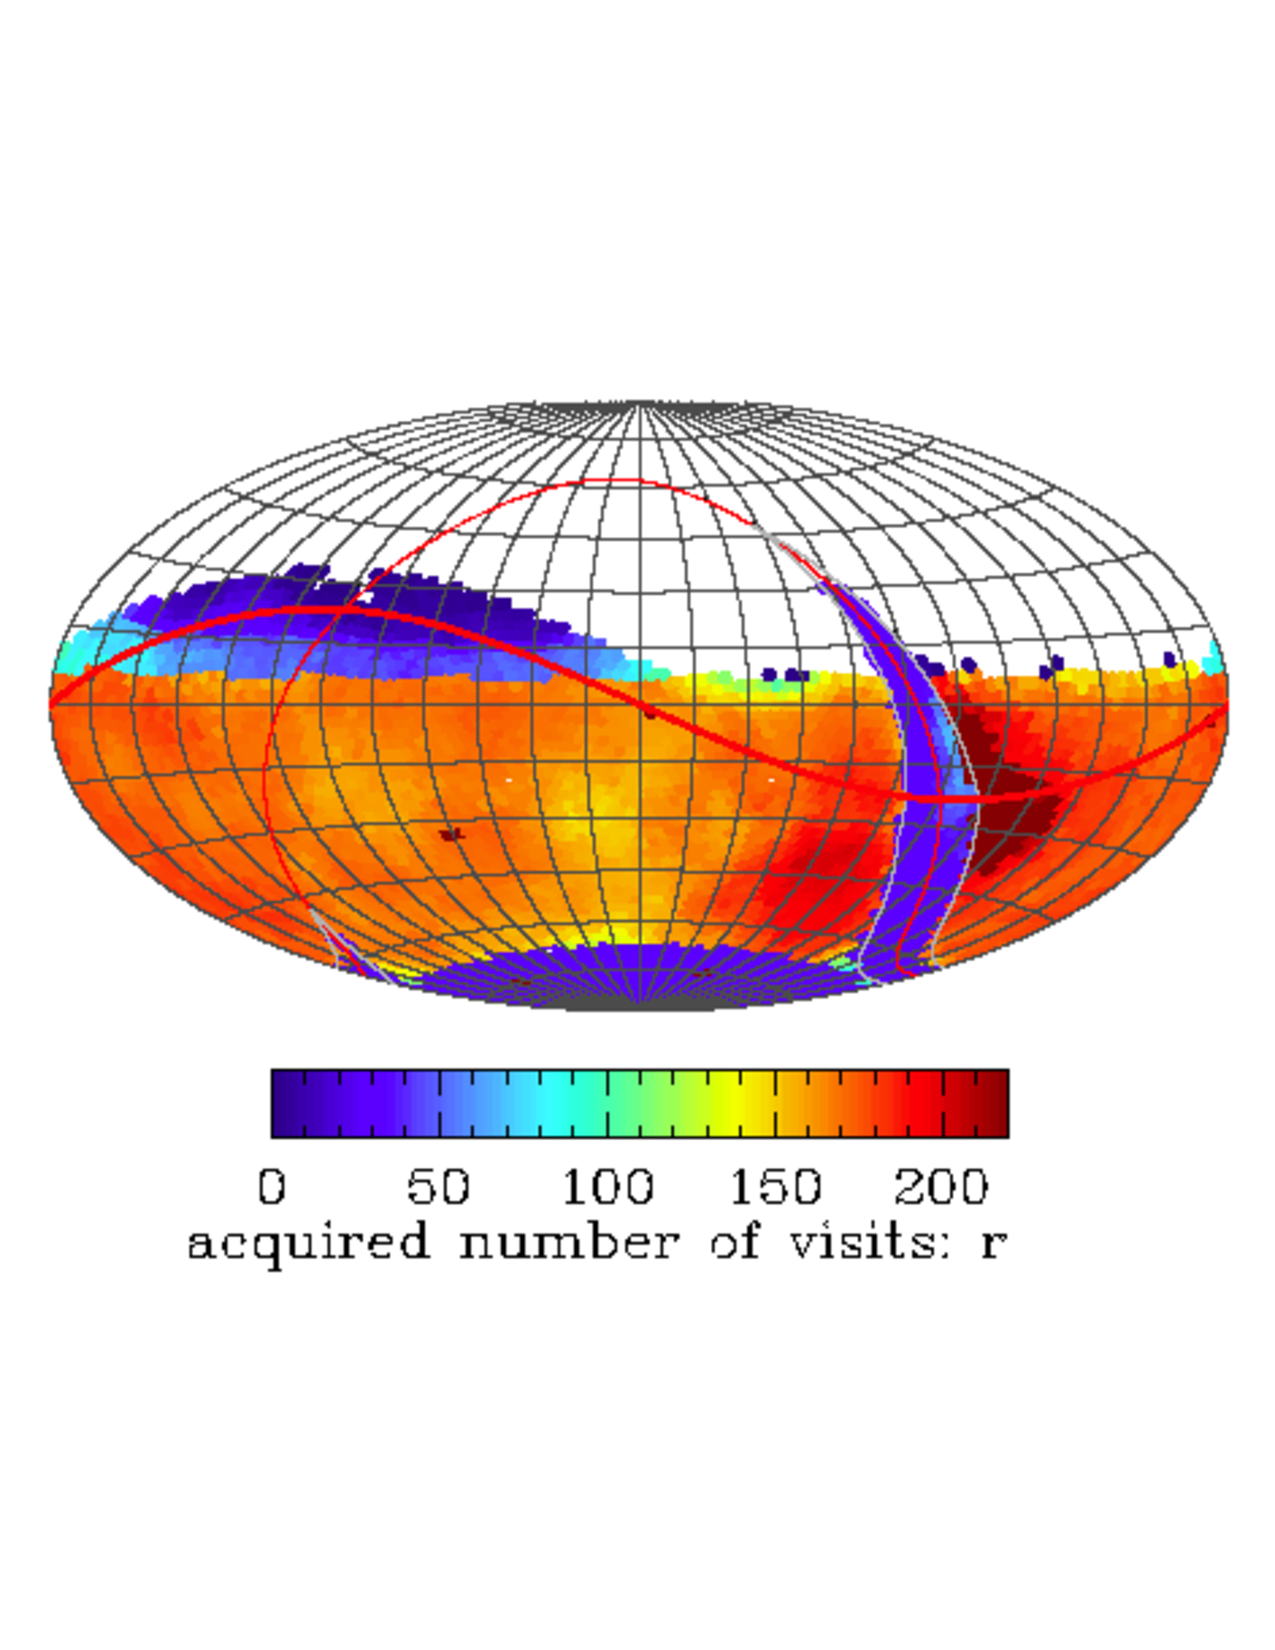
\includegraphics[width=1.0\hsize,clip]{rBandWhite.pdf}
\vskip -1.0in
\caption{The distribution of the $r$ band visits on the sky for one simulated 
realization of the baseline main survey. The sky is shown in Aitoff projection 
in equatorial coordinates (the vernal equinoctial point is in the center, and 
the right ascension is increasing from right to left) and the number of visits for 
a 10-year survey is color-coded according to the inset. The three regions with 
smaller number of visits than the main survey (``mini-surveys'') are the Galactic 
plane (arc on the right), the so-called ``northern Ecliptic region'' (upper left), and
the region around the South Celestial Pole (bottom).} 
\label{Fig:rbandSky}
\end{figure}

The observing strategy for the main survey will be optimized for the homogeneity
of depth and number of visits. In times of good seeing and at low airmass, preference 
is given to $r$-band and $i$-band observations. As often as possible, each field will be 
observed twice, with visits separated by 15-60 minutes. This strategy will provide motion 
vectors to link detections of moving objects in the Solar System, and fine-time sampling 
for measuring short-period variability. The ranking criteria also ensure that the 
visits to each field are widely distributed in position angle on the sky and 
rotation angle of the camera in order to minimize systematic effects in galaxy shape 
determination.

The universal cadence provides most of LSST's power for detecting Near Earth 
Objects (NEO) and naturally incorporates the southern half of the ecliptic 
within its 20,000 square degrees (the northern half lies above the desired airmass 
limits, $X\la1.5$). NEO survey completeness for the smallest bodies ($\sim$140m in 
diameter, per the Congressional NEO mandate) is greatly enhanced, however, by the 
addition of a crescent on the sky within 10 degrees of the northern ecliptic
(see Fig.~\ref{Fig:rbandSky}). Thus, the ``northern Ecliptic proposal'' (here ``proposal''
refers to an observing program) extends the universal cadence to this region using the
$r$ and $i$ filters only, along 
with more relaxed limits on airmass and seeing. Relaxed limits on airmass and 
seeing are also adopted for $\sim$700 deg$^2$ around the South Celestial 
Pole, allowing coverage of the Large and Small Magellanic Clouds.

Finally, the universal cadence proposal excludes observations in a region of 
1,000 square degrees around the Galactic Center, where the high stellar
density leads to a confusion limit at much brighter magnitudes than those 
attained in the rest of the survey. Within this region, the Galactic Center
proposal provides 30 observations in each of the six filters, distributed 
roughly logarithmically in time (it may not be necessary to use the
$u$ and $g$ filters for this heavily extincted region). 

The resulting sky coverage for the LSST baseline
cadence, based on detailed operations simulations, is shown for the 
$r$ band in Fig.~\ref{Fig:rbandSky}. The anticipated total number of visits 
for a ten-year LSST survey is about 2.8 million ($\sim$5.6 million 15-second long
exposures). The per-band allocation of these visits is shown in Table 1.



\subsubsection{ Mini-surveys}
\label{Sec:minisurveys}

Although the uniform treatment of the sky provided by the universal cadence
proposal can satisfy the majority of LSST scientific goals, roughly 10\%
of the time will be allocated to other strategies that significantly enhance the 
scientific return.  These surveys aim to extend the parameter space accessible 
to the main survey by going deeper or by employing different time/filter
sampling. 

As an example of a mini-survey, consider a program that uses one hour of
observing time per night to observe a relatively small region of sky to
substantially greater depth in individual visits. Accounting for
read-out time and filter changes, it could obtain about 50 consecutive
15-second exposures in each of four filters in an hour. If a field is visited
every two days over four months, about 600 deg$^2$ can be observed with this 
cadence over 10 years. Taking weather into account, the selected fields would 
each have on average about 40 hour-long sequences of 200 exposures each. Each 
observation in a sequence would have an equivalent 5-$\sigma$ depth of
$r\sim24$, and each filter subsequence when coadded would be 2 magnitudes 
deeper than the main survey visits ($r\sim26.5$). When all 40 sequences and 
the main survey visits are coadded, they would extend the depth to $r\sim28$. 

This data set would be excellent for a wide variety of science programs. The 
individual sequences would be sensitive to 1\% variability on hourly time 
scales, allowing discovery of planetary eclipses. If these fields were selected 
at Galactic latitudes of $|b|\sim30$ deg, they would include about 10 million 
stars with $r<21$ observed with signal-to-noise ratio above 100 in each visit.
When subsequences from a given night were coadded, they would 
provide dense time sampling to a faint limit of $r\sim26.5$ (assuming observations
in 4 bands, every 2 days over 120 days, and accounting for weather losses), and thus 
enable deep searches 
for SN, trans-Neptunian objects, and other faint transient, moving and 
variable sources.  For example, the SN sample
would be extended to redshifts of $z\sim1.2$, with more densely sampled light
curves than obtained from the universal cadence. Such sequences would also
serve as excellent tests of our photometric calibration procedures. 


The baseline universal cadence is by no means the definitive plan for the entire
survey. Rather, it represents a proof of concept that it is indeed possible to 
design a universal cadence which addresses a wide variety of science goals in a nearly 
optimal way. We are undertaking a vigorous and systematic research effort to explore 
the enormously large parameter space of possible surveys. The commissioning period 
will be used to test the usefulness of various observing modes and to explore 
alternative strategies. Proposals from the community, through the science collaborations
(see \S~\ref{Sec:community}), for specialized cadences (such as mini-surveys and
micro-surveys) will also be considered.  



\begin{table}
\caption{The Parameters From Eqs.~\ref{ggg} and \ref{m5}}
\begin{tabular}{|r|r|r|r|r|r|r|}
\hline  
              &   $u$  &   $g$   & $r$   &  $i$  & $z$  & $y$  \\
\hline  
   $m_{\rm sky}^a$ &   22.9    & 22.3    & 21.2    & 20.5    & 19.6    &  18.6  \\
   $\theta^b$      &   0.77    & 0.73    & 0.70    & 0.67    &  0.65   &  0.63  \\
  $\gamma^c$       &   0.037   & 0.038   & 0.039   & 0.039   & 0.040   & 0.040 \\
  $C_m^d$        &   23.05   & 24.40   & 24.60   & 24.22   & 23.92   & 23.17 \\
    $k_m^e$       &    0.451   &  0.163   &  0.087   &  0.065   &  0.043   &  0.138 \\
    $m_5^f$        &   23.9    & 25.0    & 24.7    &  24.0   & 23.3    & 22.1  \\
    $\Delta m_5^g$ &   0.21    & 0.15   & 0.14    &  0.13   & 0.13    & 0.15  \\
\hline                         
\end{tabular}
  \\ \vskip 0.05in
  $^a$ The expected median zenith sky brightness at Cerro Pach\'on, derived 
       from the median dark sky brightness observed by SDSS (AB mag arcsec$^{-2}$). \\
  $^b$ The expected delivered median zenith seeing (arcsec). For larger
       airmass, $X$, seeing is proportional to $X^{0.6}$. \\
  $^c$ The band-dependent parameter from Eq.~\ref{ggg}. \\
  $^d$ The band-dependent parameter from Eq.~\ref{m5}. \\
  $^e$ Adopted atmospheric extinction. \\
  $^f$ The typical 5$\sigma$ depth for point sources at zenith, assuming exposure time of 
       2$\times$15 sec, and observing conditions as listed. For larger
       airmass the 5$\sigma$ depth is brighter; see the bottom row. \\
  $^g$ The loss of depth at the median airmass of $X=1.2$ due to seeing degradation 
       and increased atmospheric extinction. \\
\end{table}



\subsection{  Detailed Analysis of Simulated Surveys  } 

As examples of analysis enabled by the Operations Simulator, we describe 
determination of the completeness of the LSST NEO survey, and estimation 
of errors expected for trigonometric parallax and proper motion measurements. 
In both examples, the conclusions crucially depend on assumed signal-to-noise
ratios, described next.

\subsubsection{  Expected Signal-to-Noise Ratio } 

The output of operations simulations is a data stream consisting of 
a position on the sky and the time of observation, together with 
observing conditions such as seeing and sky brightness. The expected 
photometric error (the inverse of the signal-to-noise ratio) for a single visit
can be written as
\begin{equation}
         \sigma_1^2 = \sigma_{sys}^2 + \sigma_{rand}^2,
\end{equation}
where $\sigma_{rand}$ is the random photometric error and $\sigma_{sys}$ is 
the systematic photometric error (includes errors due to, e.g., imperfect
modeling of the point spread function, but does not include errors in 
absolute photometric zeropoint). The calibration system and procedures
are designed to maintain $\sigma_{sys}<0.005$ mag. Based on 
SDSS experience (Sesar et al. 2007), the random photometric error, as
a function of magnitude, is well described\footnote{Eq.~\ref{ggg} can 
be derived from $\sigma_{rand}=N/S$, where $N$ is noise and $S$ is signal, 
and by assuming that $N^2 = N_o^2 + \alpha S$. The constants $N_o$ and 
$\alpha$ can be expressed in terms of a single unknown constant $\gamma$ 
by using the condition that $\sigma_{rand}=0.2$ for $m=m_5$.} by
\begin{equation}
\label{ggg}
  \sigma_{rand}^2 = (0.04-\gamma)\, x + \gamma \, x^2 \,\,\, {\rm (mag^2),}
\end{equation}
with $x = 10^{0.4\,(m-m_5)}$. Here $m_5$ is the 5$\sigma$ depth (for
point sources) in a given band, and $\gamma$ depends on the sky 
brightness, readout noise, etc. Using the LSST exposure time 
calculator\footnote{Available at http://dls.physics.ucdavis.edu/etc.} 
(Gee et al. 2007), we have obtained the values of $\gamma$ 
listed in Table 2. The 5$\sigma$ depth for point sources is determined from 
\begin{eqnarray}
\label{m5}
  m_5 = C_m + 0.50\,(m_{sky}-21) + 2.5\,\log_{10}(0.7/\theta) +  \nonumber \\
        + 1.25\,\log_{10}(t_{vis}/30) - k_m(X-1) \phantom{xxxxx}
\end{eqnarray}
where $m_{sky}$ is the sky brightness (AB mag arcsec$^{-2}$), $\theta$ is 
the seeing (FWHM, in arcsec), $t_{vis}$ is the exposure time (seconds),
$k$ is the atmospheric extinction coefficient, and $X$ is airmass. 
The constants $C_m$ depend on the overall throughput of the instrument
and are 
\B{computed from the design requirements for $m_5$ listed in the
LSST Science Requirements Document. The available throughput data for
optical elements and sensors are consistent with the resulting $C_m$ values 
listed in Table 2, and the differences in performance between LSST and,
for example, SDSS are easily understood\footnote{SDSS data 
typically reach a 5$\sigma$ depth for point sources of $r=22.5$ 
with an effective aperture of $D=2.22$m, an exposure time of $t_{vis}=54$ 
sec, the median $r$ band sky brightness of $r_{sky}=20.9$ mag arcsec$^{-2}$, 
the median seeing of $\theta=1.5$ arcsec, and the median airmass of $X=1.3$.
In comparison, the LSST loss of depth is 0.32 mag due to shorter exposures,
while the gains are 1.17 mag due to larger aperture, 0.83 mag due to better 
seeing, 0.20 mag due to fainter sky, and 0.10 mag due to better throughput,
for the net gain of $\sim$2.0 mag.}.}


\subsubsection{   The NEO Completeness Analysis    } 
\label{Sec:NEOc}
To assess the LSST completeness for PHAs, the PHA 
population is represented by a size-limited complete sample of 800 true
PHAs whose orbital elements are taken from the Minor Planet Center.
The simulated baseline survey is used to determine which PHAs are present in
each exposure and at what signal-to-noise ratio they were observed. In 
addition to  seeing, atmospheric transparency, and sky background effects
(see eq.~\ref{m5}), the signal-to-noise computation takes into account losses 
due to non-optimal filters and object trailing. Using SDSS observations
of asteroids (Ivezi\'c et al. 2001), we adopt the following mean colors to 
transform limiting (AB) magnitudes in LSST bandpasses (listed in Table 2)
to an `effective'' limiting magnitude in the standard $V$ band: 
$V-m=(-2.1, -0.5, 0.2, 0.4, 0.6, 0.6)$ for $m=(u,g,r,i,z,y)$. Due to 
very red $V-u$ colors, and the relatively bright limiting magnitude in the $y$ 
band, the smallest objects are preferentially detected in the $griz$ bands.
The correction for trailing is implemented by subtracting from the right-hand 
side of eq.~\ref{m5}
\begin{equation}
 \Delta m_5^{\rm trailing} = 1.25\,\log_{10}(1+0.0267{v \,t_{vis} \over \theta}),
\end{equation}
where the object's velocity, $v$, is expressed in deg.~day$^{-1}$. For the nominal
exposure time of 30 seconds and $\theta=0.7$ arcsec, the loss of limiting 
magnitude is 0.16 mag for $v=0.25$ deg.~day$^{-1}$, typical for objects in the main 
asteroid belt, and 0.50 mag for $v=1.0$ deg.~day$^{-1}$, typical of NEOs passing
near Earth. 

Above 60\% completeness, one magnitude of depth is roughly
equivalent to 10\% in completeness.  An object's orbit is considered to be 
cataloged if the object was detected on at least three nights during a single 
lunation, with a minimum of two visits per night. The same criterion
was used in NASA studies\footnote{The NASA 2007 NEO study is available from
http://neo.jpl.nasa.gov/neo/report2007.html.}, and is confirmed as
reliable by a detailed analysis of orbital linking and determination using
the MOPS code (Jedicke et al. 2005) developed by the Pan-STARRS project (and 
adopted by LSST in a collaborative effort with Pan-STARRS). The MOPS software
system and its algorithms are significantly more advanced than anything
fielded for this purpose to date. Realistic MOPS simulations show 
$>$99\% linking efficiency across all classes of solar system objects. 
For the LSST baseline cadence, objects
counted as cataloged are observed on 20 different nights on average over ten
years. A more stringent requirement that an object must be detected on at least 
five nights decreases the completeness by typically 3\%. The completeness is also a
function of the assumed size distribution of NEOs: the flatter the distribution, the 
higher the completeness. If the latest results for the NEO size
distribution by A. Harris (priv. comm.) are taken into account, the
completeness increases by 1-2\%. Due to these issues, the completeness
estimates have a systematic uncertainty of at least 2\%. 

The LSST baseline cadence provides orbits for 82\% of PHAs larger than 140
meters after 10 years of operations. With a minor change of this cadence, such as
requiring that all observations in the so-called NE region (North Ecliptic 
region, defined by $\delta >+5^\circ$) are obtained in the $r$ band, the completeness 
for 140m and larger PHAs is 84\%, with 90\% completeness reached for 200m and 
larger objects. The completeness curve as a function of an object's size is shown 
in Fig.~\ref{Fig:Cneo} (lower curve). This cadence spends 5\% of the total 
observing time on NEO-optimized observations in the NE region. 



\begin{figure}
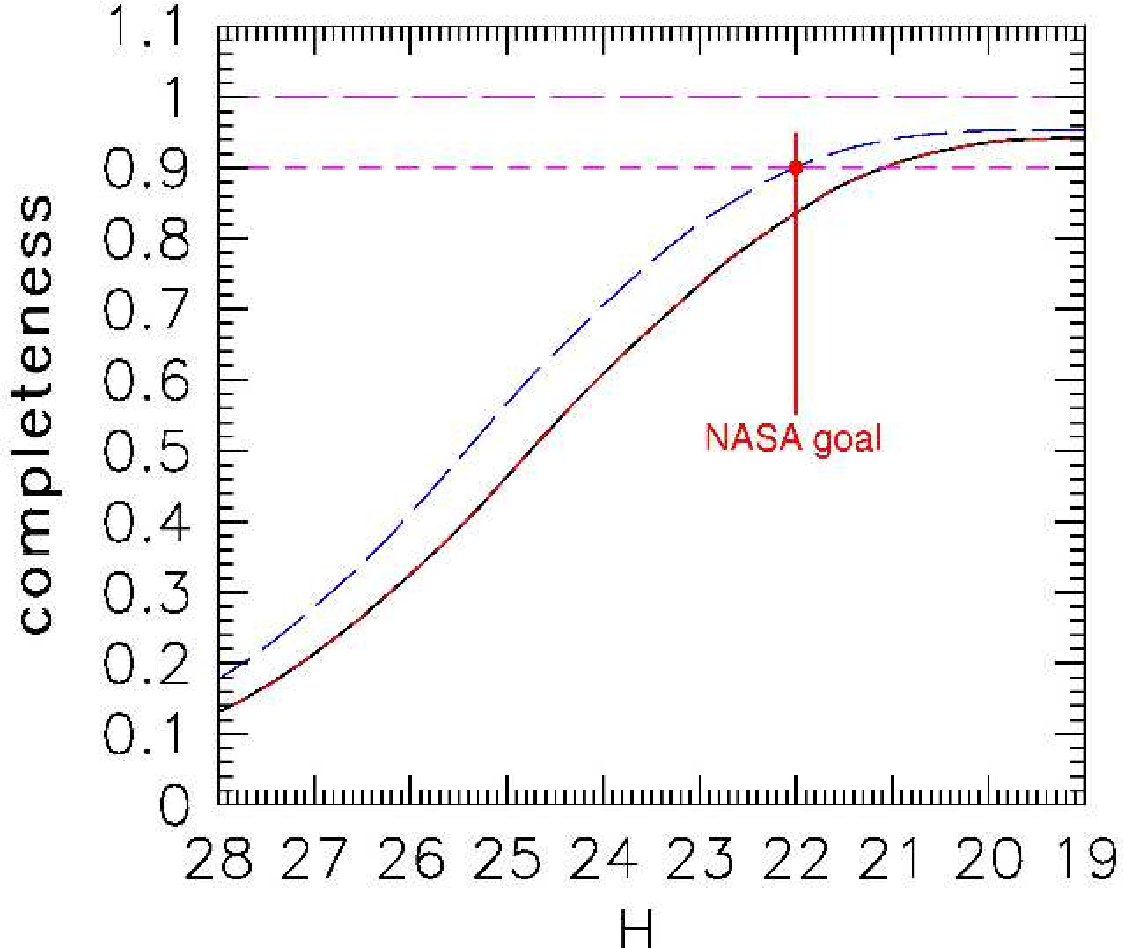
\includegraphics[width=1.0\hsize,clip]{Cneo.pdf}
\caption{Completeness of the LSST survey for PHAs brighter than a given absolute
magnitude (related to the size of the object and albedo; 
$H$=22 mag is equivalent to a typical 140m asteroid and $H$=24 mag is
equivalent to a 50m asteroid). Two scenarios are shown: the lower curve is the 
10-year long baseline survey with a 5\% NEO optimization, and it reaches a 
completeness of 84\%. The upper dashed curve results from spending 15\% of the 
observing time in an NEO optimized mode, and running the survey for 12 years.  
It meets the 90\% completeness level for 140m objects mandated by the Congress.} 
\label{Fig:Cneo}
\end{figure}

Various adjustments to the baseline cadence can boost the completeness for
140m and larger PHAs to 90\%. We find that such variations can have an unacceptably 
large impact on other science programs, if the 90\% completeness is to be reached 
within the 10 year survey lifetime. However, with a minor adjustment of the 
baseline cadence, such that 15\% of the time is spent in the NE region to reach
fainter limiting magnitudes, this completeness level can be reached with a 12-year 
long survey, and with a negligible effect on other science goals. The completeness 
curve as a function of an object's size for such a modified cadence is shown in 
Fig.~\ref{Fig:Cneo} (upper curve).

Our analysis assumes that no NEOs are known prior to LSST. Currently known
NEOs do not have a significant impact on this calculation. However, if a precursor 
survey, such as Pan-STARRS 4, operated for three years prior to LSST, the time to
fulfill the Congressional mandate by LSST could be shortened by about a year.


\subsubsection{The Expected Accuracy of Trigonometric Parallax and Proper Motion Measurements } 

%\vskip -0.1in
Given the observing sequence for each sky position in the main survey, we
generate a time sequence of mock astrometric measurements. The assumed astrometric 
accuracy is a function of signal-to-noise ratio. Random astrometric errors per
visit are modeled as $\theta/SNR$, with $\theta=700$ mas and $SNR$ determined using
eq.~\ref{m5}. The estimated proper motion and parallax accuracy at the bright end
($r<20$) is driven by systematic errors due to the atmosphere. Systematic
errors of 10 mas are added in quadrature, and are assumed to be {\it uncorrelated} 
between different observations of a given object. Systematic and random
errors become similar at about $r=22$, and there are about 100 stars per LSST 
sensor (0.05 deg$^2$) to this depth (and fainter than the LSST saturation limit at
$r\sim16$) even at the Galactic poles. 

Data from the Subaru telescope indicate that systematic errors of 
10 mas on spatial scales of several arcminutes are realistic. Even a drift-scanning 
survey such as SDSS delivers uncorrelated systematic errors (dominated by seeing 
effects) at the level of 20-30 mas (measured from repeated scans; Pier et al. 2003);
the expected image quality for LSST will be twice as good as for SDSS. Furthermore, 
there are close to 1000 galaxies per sensor with $r<22$, which will provide exquisite 
control of systematic astrometric errors as a function of magnitude, color and other 
parameters, and thus enable absolute proper motion measurements.

The astrometric transformations for a given CCD and exposure, and 
proper motion and parallax for all the stars from a given CCD, are simultaneously
solved for using an iterative algorithm. The astrometric transformations from
pixel to sky coordinates are modeled using low-order polynomials and standard
techniques developed at the U.S. Naval Observatory (Monet et al. 2003). The expected 
proper motion and 
parallax errors for a 10-year long baseline survey, as a function of apparent 
magnitude, are summarized in Table 3. Blue stars (e.g., F/G stars) fainter than 
$r\sim23$ will have about 50\% larger proper motion and parallax errors than 
given in the table due to decreased numbers of $z$ and $y$ band detections. The 
impact on red stars is smaller due to a relatively small number of observations 
in the $u$ and $g$ bands, but extremely red objects, such as L and T dwarfs, 
will definitely have larger errors, depending on details of their spectral 
energy distributions.  After the first three years of the survey, 
{\it the proper motion errors will be about five times as large, and parallax
errors will be about twice as large,} as the values given in Table 3; the errors
scale as $t^{-3/2}$ and $t^{-1/2}$, respectively. This error behavior is 
a strong independent argument for a survey lifetime of at least 10 years 
(c.f. \S 2).  




\begin{table}
\caption{The expected proper motion, parallax and accuracy for a 10-year long baseline survey.}
\begin{tabular}{|l|c|c|c|c|c|}
\hline  
    $r$   &  $\sigma^a_{xy} $  & $\sigma^b_\pi$  &   $\sigma^c_\mu$   &  $\sigma^d_1$  &  $\sigma^e_C$  \\
    mag &       mas            &      mas  & mas/yr &   mag   &    mag  \\
\hline  
       21 &  11  &  0.6  &  0.2   &   0.01  &   0.005 \\
       22 &  15  &  0.8  &  0.3   &   0.02  &   0.005 \\
       23 &  31  &  1.3  &  0.5   &   0.04  &   0.006 \\
       24 &  74  &  2.9  &  1.0   &   0.10  &   0.009 \\
\hline                         
\end{tabular}
\\ \vskip 0.05in
  $^a$ Typical astrometric accuracy (rms per coordinate per visit); \\
  $^b$ Parallax accuracy for 10-year long survey; \\
  $^c$ Proper motion accuracy for 10-year long survey; \\
  $^d$ Photometric error for a single visit (two 15-second exposures); \\
  $^e$ Photometric error for coadded observations (see Table 1). \\
\end{table}



For comparison with Table 3, the SDSS-POSS proper motion measurements have an 
accuracy of $\sim$5 mas yr$^{-1}$ per coordinate at $r=20$ (Munn et al. 2004). Gaia
is expected to deliver parallax errors of 0.3 mas and proper motion errors of 
0.2 mas yr$^{-1}$ at its faint end at $r\sim20$ (Perryman et al. 2001). Hence, LSST will smoothly 
extend Gaia's error vs. magnitude curve 4 magnitudes fainter.



\subsection{             Data Products                    } 

\subsubsection{ Standard processing and data products}

The LSST data system is being designed to enable as wide a range of science as 
possible. Standard data products, including calibrated images and catalogs of
detected objects and their attributes, will be provided both for individual 
exposures and the deep incremental data coaddition. About 2 billion objects 
will be routinely monitored for photometric and astrometric changes, and any 
transient events (non-recurrent objects with statistically significant photometric 
change; about 10,000 per night on average) will be posted in less than 60 seconds 
via web portals including the Virtual Observatory. 
For the ``static'' sky, there will be yearly database releases listing many 
attributes for billions of objects. This database will grow in size to about 
30 PB and about 20 billion objects\footnote{It is assumed that about 10 billion stars
and 10 billion galaxies will be detected by LSST. The estimate of about 10 billion
detected stars is sensitive to assumptions about the distribution of the 
interstellar dust in the Galactic plane, and cadence details. Plausible variations
in these assumptions yield stellar samples 
ranging from 5 billion to 20 billion stars.} in ten years, and will 
include other metadata (parameter error estimates, system data, seeing
summary, etc). For a comparison, the SDSS Data Release 7 imaging database
includes about 357 million unique objects\footnote{http://www.sdss.org/dr7/}. 

The SDSS experience is that the distribution of sizes of data portal requests 
follows a power law, ranging from frequent simple queries or image cutout
downloads to infrequent major downloads or large calculations. The same 
distribution is expected for LSST, and we are designing the system to enable this 
entire distribution. This data archive server will involve different resources deployed 
in different ways. We plan to optimize the mix by shipping algorithms to the data 
for those cases that need it (and offering local parallel computation) and 
transferring the data to the user for other use cases. While the data archive will 
be at the National Center for Supercomputing Applications at the University of
Illinois, we plan multiple data portals for community access to both the 
pixel data and the database. We are designing for a wide range of queries and 
access patterns in order to serve the broadest range of scientists, as well as 
interested amateurs. The LSST database will be inter-operable with those of 
surveys in other wavebands, via the Virtual Observatory. 


\subsubsection{ Non-standard data processing and data access}

The database is designed to allow evolution in the nature of the science queries. 
This design is more than simply configuring it
to allow for expected growth in query complexity with time. For
example, we anticipate that some users will submit queries on the images 
themselves. We plan for two pathways outside of the database query system
for non-standard pixel processing. The first is through a pipeline interface
that would allow a user group to attach their own pipeline processing system
at a Data Access Center. This approach is appropriate for major undertakings 
such as a weak lensing analysis starting at the image level,
or new ways to coadd the data. The second approach is simply to include the 
desired processing, such as a new quantity to be included in the Object database, 
within the data release processing, and execute it on the next data release 
run. Much of the science will be statistical in nature and will involve large 
correlation calculations with user-specified precision. We plan to enable
open source community-driven applications development. Finally, special data 
pipelines developed by the Science Collaborations (see \S~\ref{Sec:community}) 
will populate new parameters in the database. 



\begin{figure}
\hskip -0.8in
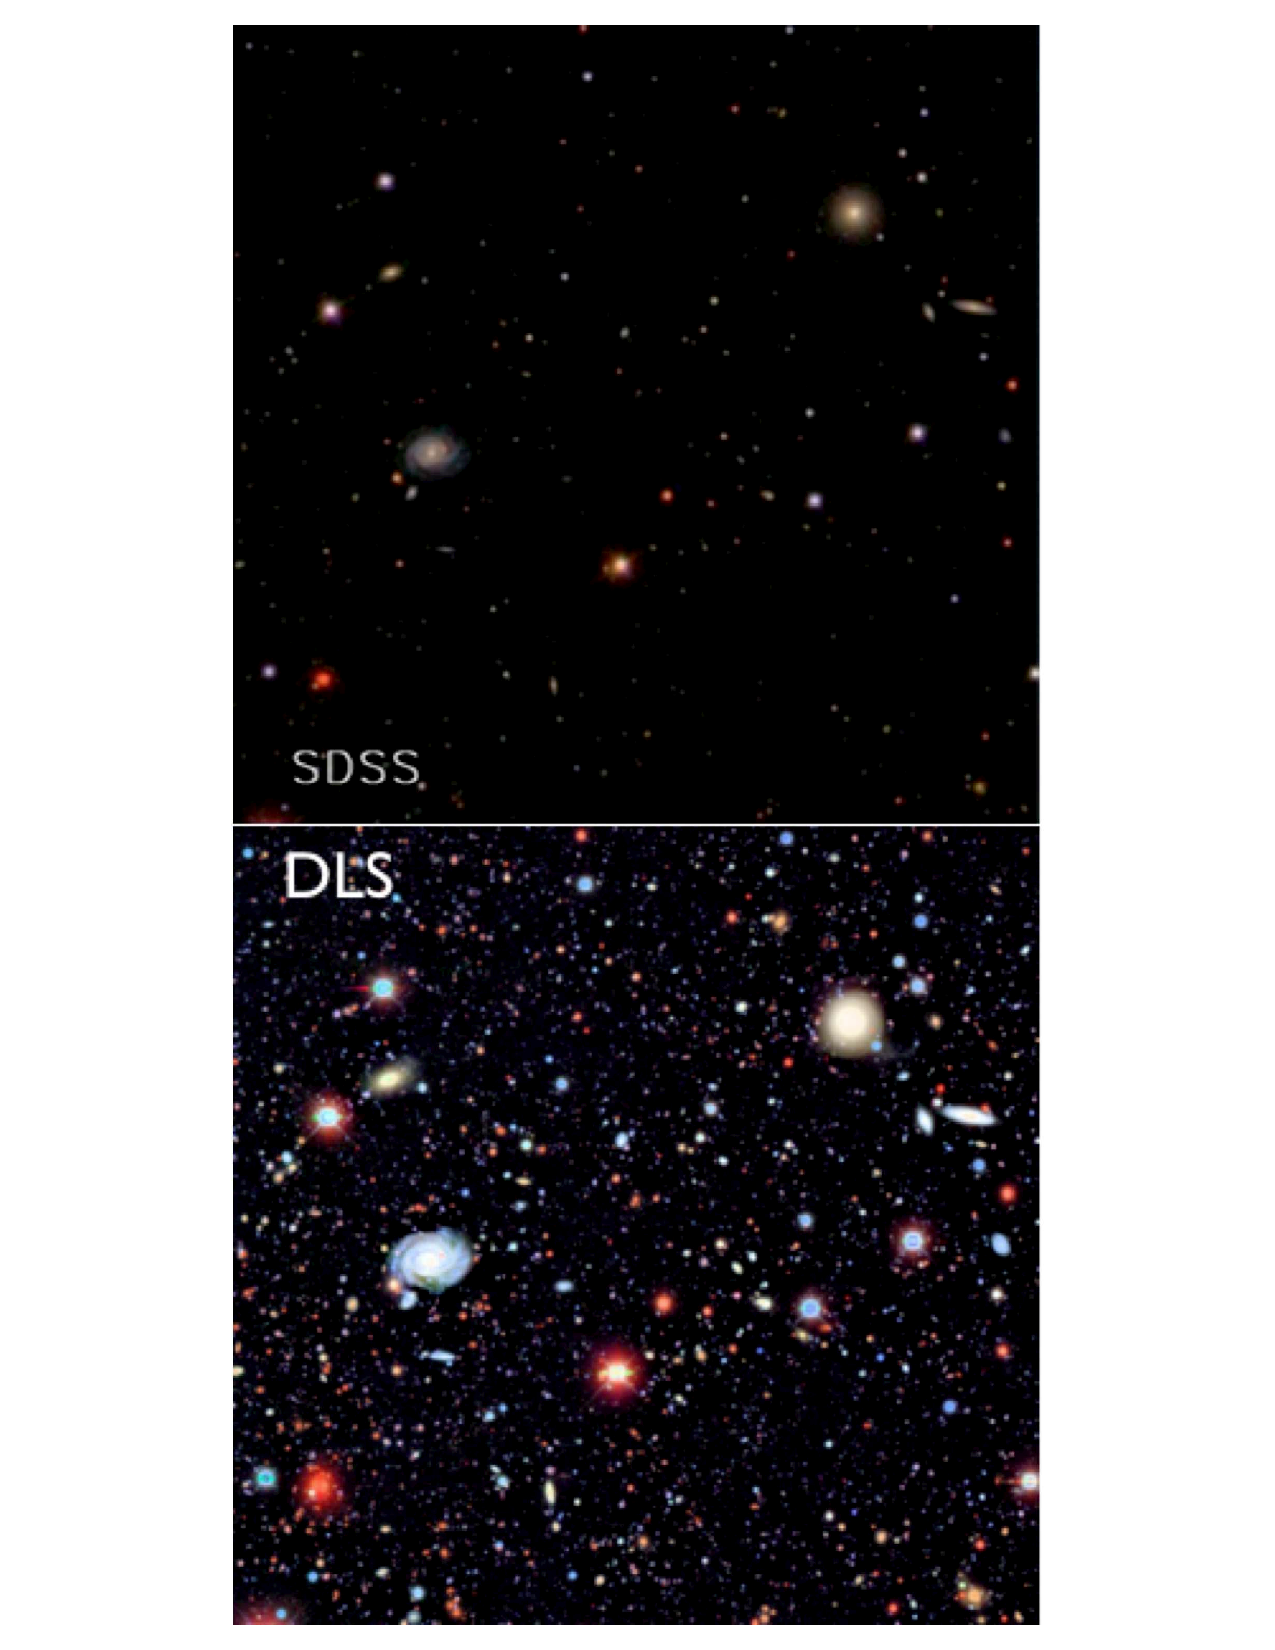
\includegraphics[width=1.5\hsize,clip]{panels1_2.pdf}
\caption{A comparison of $\sim7.5\times7.5$ arcmin$^2$ images of
the same area of sky (centered on $\alpha$=9$^h$ 20' 47'' and 
$\delta$=30$^\circ$ 8' 12'') obtained by the SDSS (top, $r<22.5$) and 
the Deep Lens Survey (bottom, $r<24.5$). The depth gain for the bottom image
is mostly due to the lower surface brightness limit, which is also responsible 
for the apparent increase of galaxy sizes. LSST will obtain $\sim$100 $gri$ 
color images to the same depth ($\sim$200 for the $riz$ composites) of each point 
over half the Celestial sphere (20,000 deg$^2$, equivalent to 1.3 million $\sim7.5\times7.5$
arcmin$^2$ regions), and with better seeing. After their coaddition, the final 
image will be another $\sim3$ mag deeper (a faint limit of $r=27.5$ for point 
sources).} 
\label{Fig:panels1}
\end{figure}

\begin{figure}
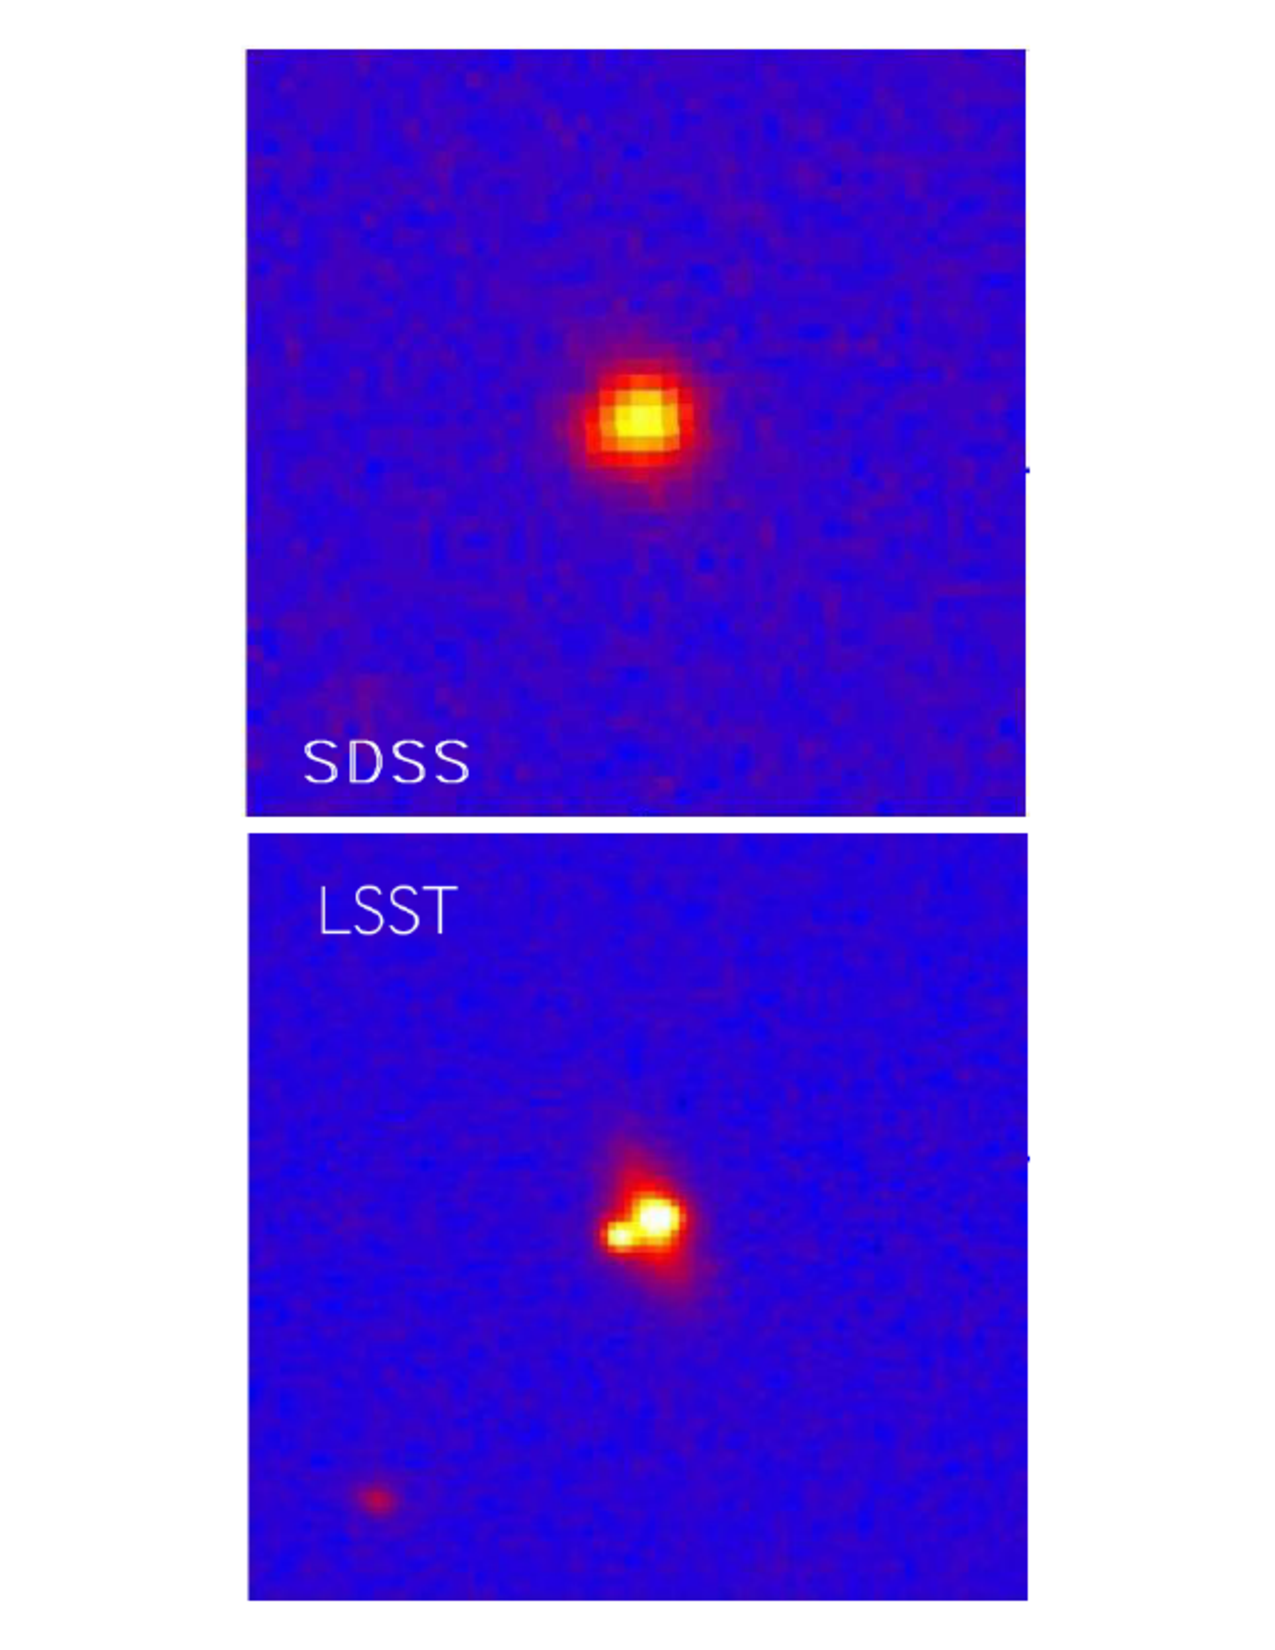
\includegraphics[width=1.0\hsize,clip]{panels2.pdf}
\caption{A comparison of angular resolution for $20\times20$ arcsec$^2$ images obtained 
by the SDSS (top, median seeing of 1.5 arcsec) and expected from LSST (bottom,
seeing of 0.7 arcsec). The images show a lensed SDSS quasar (SDSS J1332+0347,
Morokuma et al. 2007); the bottom image was taken with Suprime-cam at Subaru. 
Adapted from Blandford et al. (2008).} 
\label{Fig:panels2}
\end{figure}



\B{
\subsubsection{Data Mining Challenges}

The characterization (unsupervised machine learning) and classification (supervised machine learning) of 
massive, multivariate data catalogs such as those generated by the LSST are major research challenges for 
data-intensive astronomy (Tyson et al. 2008b; Ivezi\'{c} et al. 2008b; Bloom et al. 2008; Borne 2008,
2009). To address these questions the statistics and machine-learning research 
communities are collaborating with LSST scientists to develop new algorithms that will enable the full 
scientific potential of the LSST, including:
\begin{itemize}
\item Rapid characterizations and probabilistic classifications for the 100,000-1,000,000 sources
          detected in difference images each night.
\item Identification of unusual classes of astronomical sources using outlier detection techniques that are 
          robust to noise and image processing defects.
\item Characterization of novel and unexpected behavior in the time domain from time series data.
\item Measurements of the clustering of stars and galaxies (including higher order statistics) using fast 
          algorithms for point processes.
\item The application of dimensionality-reduction techniques to determine important physical correlations 
          within large multi-variate catalogs.
\item Model or hypothesis testing that can verify existing (or generate new) astronomical hypotheses with 
          strong statistical confidence, using millions of training samples.
\end{itemize}

The broad range of science that will benefit from statistically rigorous and computationally efficient algorithms 
has led to the creation of the Informatics and Statistical Science Research Collaboration for the LSST
 (see \S~\ref{Sec:community}) . This 
collaboration's goal is to develop, implement, and validate data mining algorithms that will scale to the size and 
complexity of the LSST data. 
}





\section{                EXAMPLES OF LSST SCIENCE PROJECTS                    }
\label{Sec:science}


The design and optimization of the LSST system leverages its unique capability 
to scan a large sky area to a faint flux limit in a short amount of time. 
The main product of the LSST system will be a multi-color $ugrizy$ image of about 
half the sky to unprecedented depth ($r\sim27.5$). For a comparison, the best 
analogous contemporary dataset is that of SDSS, which provides $ugriz$ images
of about a quarter of the sky to $r\sim22.5$, with twice as large seeing
(see Figs.~\ref{Fig:panels1} and \ref{Fig:panels2}). A major advantage of LSST 
is the fact that this deep sky map will be produced by taking hundreds of
shorter exposures (see Table 1). Each sky position within the main survey area 
will be observed about 1000 times, with time scales spanning seven orders of 
magnitude (from 30 sec to 10 years), and produce over {\it a trillion 
photometric measures} of celestial sources.

It is not possible to predict all the science that LSST data will enable.
We now briefly discuss a few projects to give a flavor of anticipated studies,
organized by the four science themes that drive the LSST design 
(although some projects span more than one theme). 
\B{For an in-depth discussion of LSST science cases, we refer the reader to the 
LSST Science Book.}
 
\begin{figure}
%\includegraphics[width=1.0\hsize,clip]{DEellipses1.pdf}
%\includegraphics[width=0.95\hsize,clip]{DEellipses2.pdf}
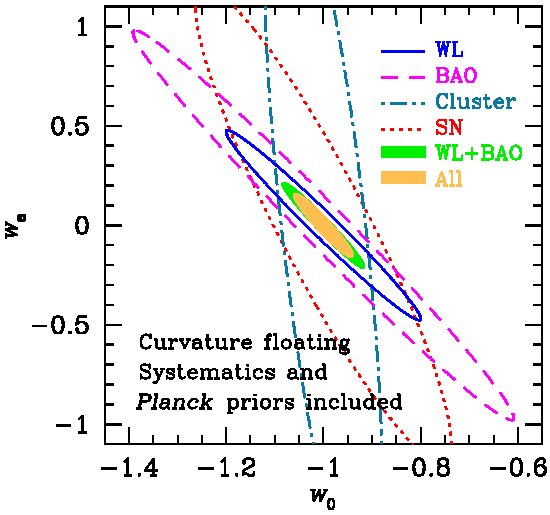
\includegraphics[width=1.0\hsize,clip]{cswb.pdf}
\caption{
LSST BAO (dashed line), cluster counting (dash-dotted line), 
supernovae (dotted line), WL (solid line), joint BAO and WL 
(green shaded area), and all combined (yellow shaded area).
The BAO and WL results are based on galaxy--galaxy, galaxy--shear,
and shear--shear power spectra only. 
Adding other probes such as strong lensing time delay
and higher-order galaxy and shear statistics will further improve 
the constraints.} 
\label{Fig:DEellipses}
\end{figure}


\vskip 0.3in
\subsection{ Probing Dark Energy and Dark Matter }

A unique aspect of LSST as a probe of dark energy and dark matter is the use of 
multiple cross-checking probes that reach unprecedented precision (see
Fig.~\ref{Fig:DEellipses}). The joint analysis of LSST weak lensing and BAO is 
particularly powerful in constraining the dynamical behavior of dark energy, 
i.e., how it evolves with cosmic time or redshift (Hu \& Jain 2004; Zhan 2006).
By simultaneously measuring the growth of large-scale structure, 
and luminosity and angular distances as functions of redshift (via weak lensing, 
BAO, SN, and cluster counting), LSST data can reveal whether the recent cosmic 
acceleration is due to dark energy or modified gravity (Lue, Scoccimarro \& Starkman 
2004; Knox, Song \& Tyson 2006; Ishak, Upadhye \& Spergel 2006; Jain \& Zhang 2008). 
Over a broad range of accessible redshifts, the simple linear model
for the dark energy equation of state is a poor representation of more
general dark energy theories. Barnard et al. 
(2008) have shown that in a high-dimensional dark energy model space, 
LSST data could lead to a hundred- to thousand-fold increase in precision over 
precursor experiments about to be undertaken, thereby confirming its status as 
a premier Stage IV experiment\footnote{See the Dark Energy Task Force report 
(Albrecht et al. 2006) for a definition of Stage IV experiments.}. 

The power and accuracy of LSST dark energy and dark matter probes are derived 
from samples of several billion galaxies and millions of Type Ia
supernovae. The nominal high-SNR galaxy sample defined by $i<25.3$ (SNR$>$20 for point
sources) will include four billion galaxies (56 arcmin$^{-2}$; the surface density of galaxies 
used for weak lensing analysis will be about 40 arcmin$^{-2}$) with a mean 
photometric redshift accuracy of 1-2\% (relative error for $1+z$), and with 
only 10\% of the sample with redshift errors larger than 4\%. The median redshift for 
this sample will be $z\sim$1.2, with the third quartile at $z\sim2$. For a 
subsample of 2 billion galaxies further constrained by flux limits in the 
$g$ and $z$ bands, the photometric redshift errors will be about two times 
smaller. It will be possible to further improve photometric redshift calibration
using non-conventional methods (Newman 2008). 


\begin{figure}
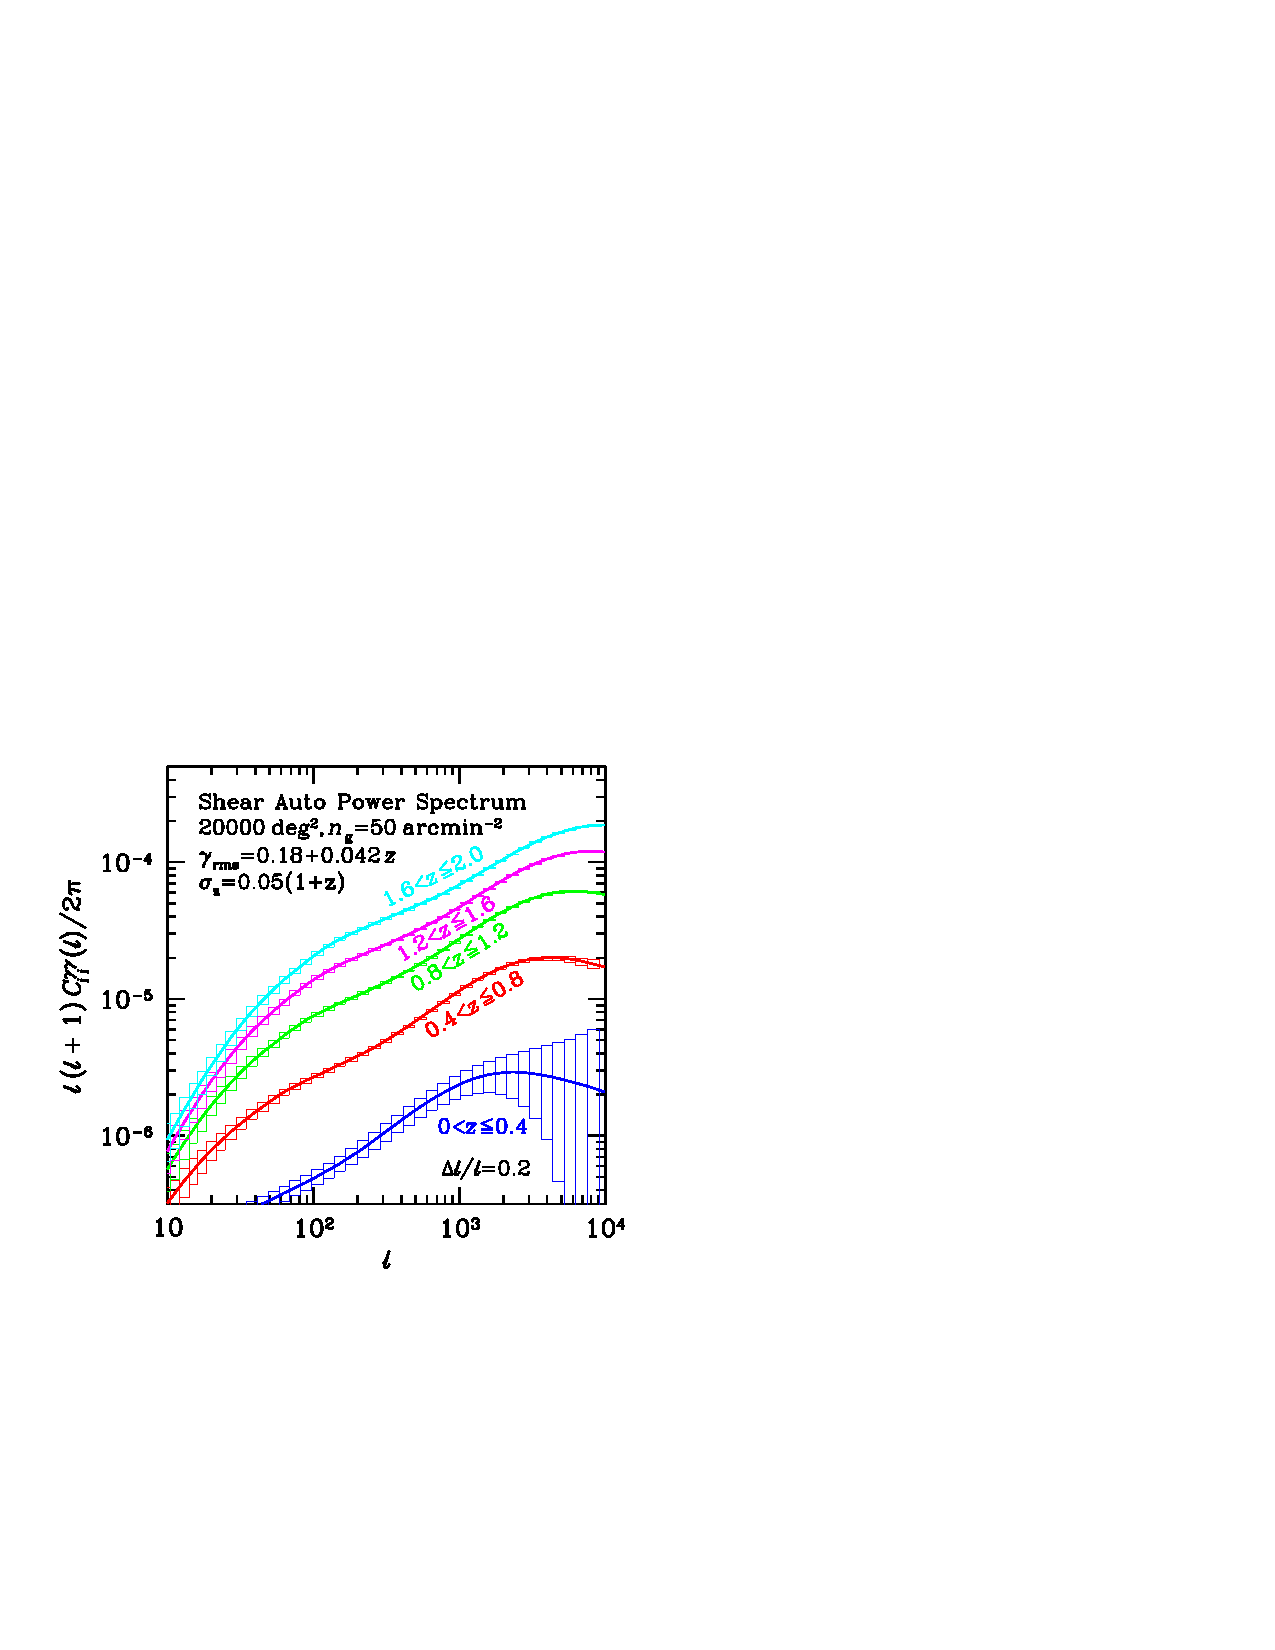
\includegraphics[width=1.0\hsize,clip]{cls.pdf}
\caption{The lensing shear auto power spectra constructed from 5 redshift bins 
($l$ is the multipole moment of the distribution on the sky). Only the 5 auto-power 
spectra of each redshift bin among the available 15 cospectra are displayed, and the 
solid curves show the predictions for the concordance $\Lambda$CDM model. The boxes 
show the expected 1-$\sigma$ measurement error ($\Delta l/l=0.2$) from the full LSST 
10-year survey due to the sample (i.e., cosmic) variance which dominates at about 
$l< 100$, and intrinsic ellipticities which dominate at $l> 1000$ (Zhan 2006).} 
\label{Fig:wlPk}
\end{figure}


\begin{figure}
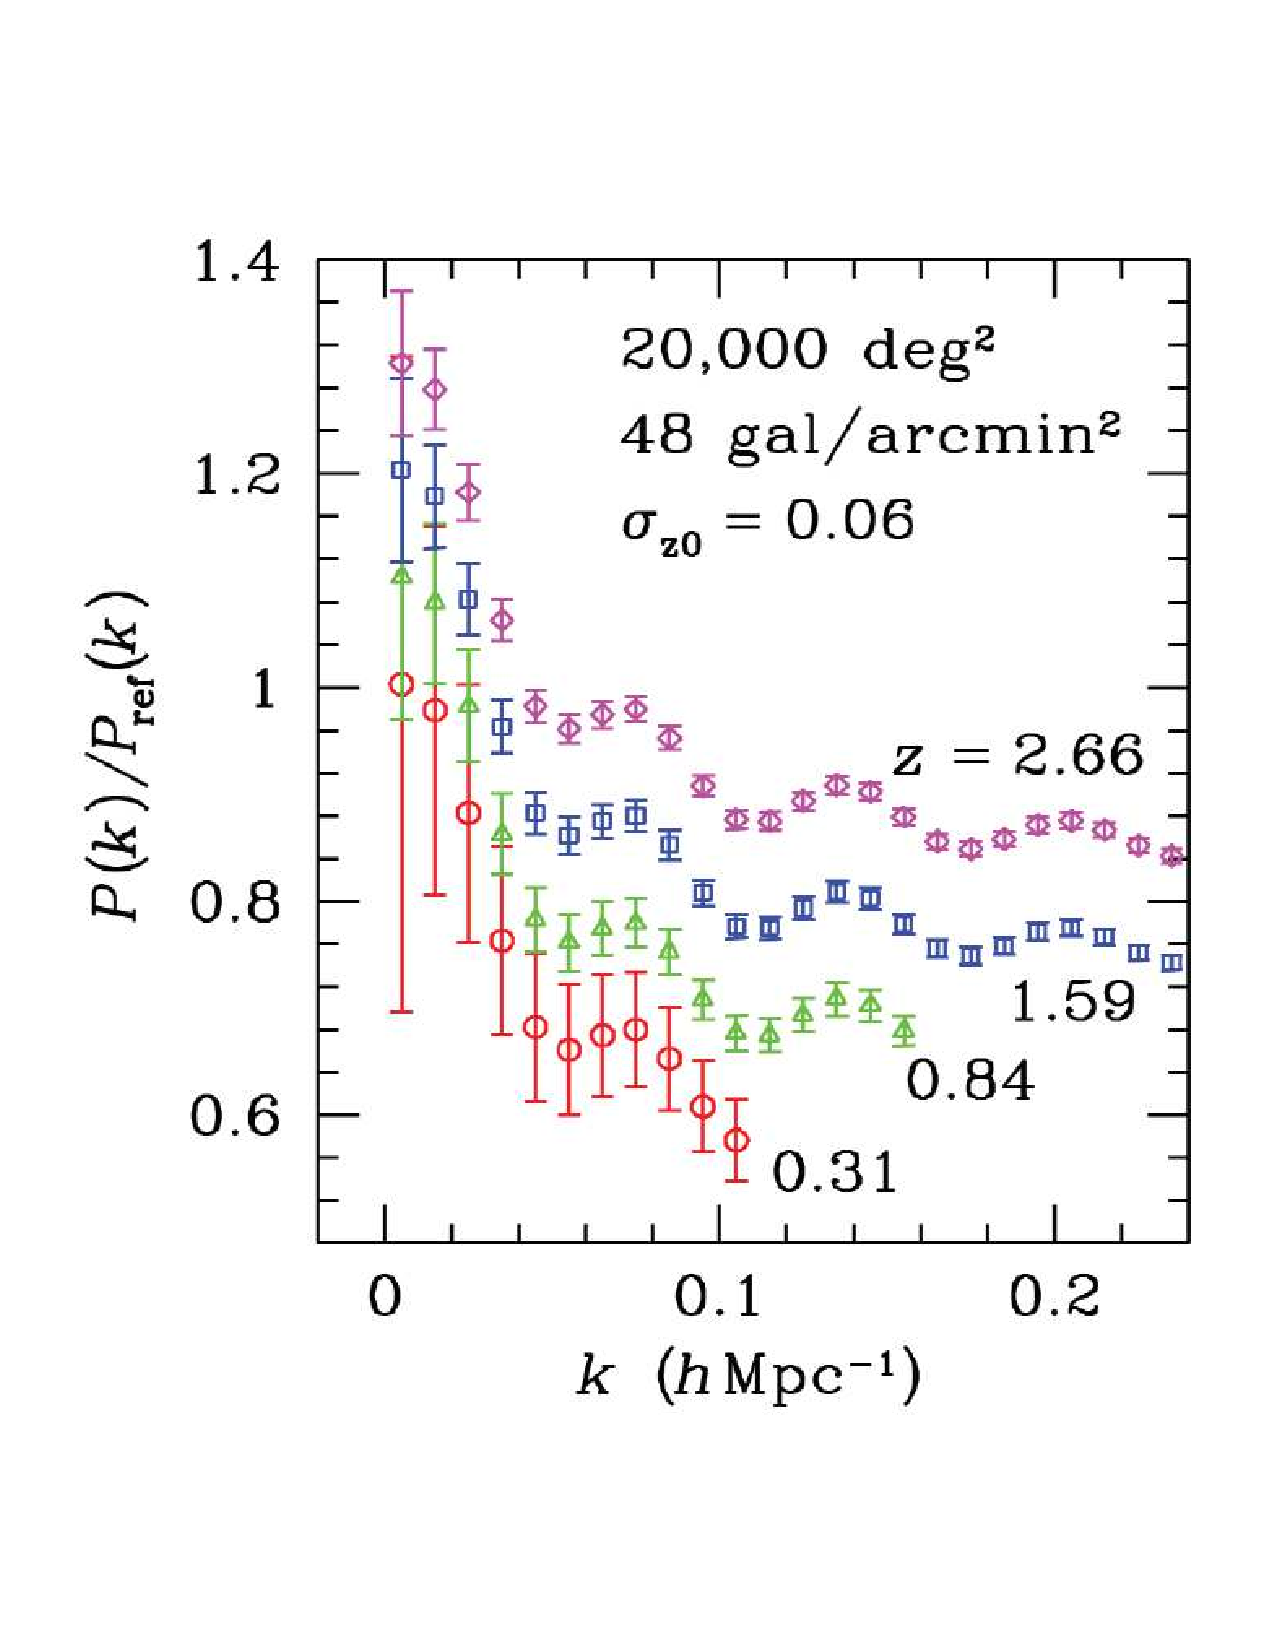
\includegraphics[width=1.0\hsize,clip]{bao.pdf}
\caption{Simulations of the ratio of the measured galaxy power spectrum to 
a featureless reference power spectrum in various redshift bins (shifted vertically 
for clarity), for the full LSST survey using conservative photometric redshift
errors. The several peaks visible in each curve are the signature of baryon acoustic 
oscillations (Eisenstein et al. 2005; Cole et al. 2005). LSST will measure the 
angular diameter distance over this redshift range with an accuracy of $\sim1$\% 
(Zhan \& Knox 2006).} 
\label{Fig:bao}
\end{figure}



\begin{figure}
%\includegraphics[width=1.0\hsize,clip]{dgcon.pdf}
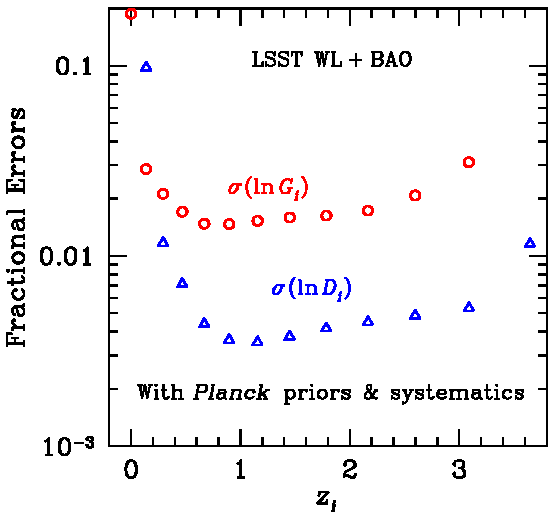
\includegraphics[width=1.0\hsize,clip]{dges.pdf}
\caption{Marginalized $1\sigma$ errors on the comoving distance 
(open triangles) and growth factor (open circles) parameters from 
the joint analysis of LSST BAO and WL (galaxy--galaxy, galaxy--shear,
and shear--shear power spectra) with a 
conservative level of systematic uncertainties in the photometric redshift error 
distribution and additive and multiplicative errors in the shear and 
galaxy power spectra. The maximum multipole used for WL is 
2000, and that for BAO is 3000 [with the additional requirement
$\Delta_\delta^2(\ell/D_{A};z) < 0.4$].
The growth parameters, $G_0 \ldots G_{14}$, are evenly spaced in 
$\log(1+z)$ between $z = 0$ and 5, and the distance parameters, 
$D_1 \ldots D_{14}$, start at $z_1 = 0.14$ (see text for details).
The error of each distance (growth) parameter is marginalized 
over all the other parameters including growth (distance) parameters. The joint constraints on 
distance are relatively insensitive to the assumed systematics
(Zhan, Knox \& Tyson 2009).} 
\label{Fig:bao2}
\end{figure}


The main LSST deliverables in the context of dark energy and matter will be

\begin{itemize}
\item Multiple cosmic two-point shear probes (Fig.~\ref{Fig:wlPk}). There will be 
over 50 of these auto and cross power spectra constructed using 3-D shear tomography 
(correlation of shear of a galaxy at one redshift bin with another galaxy in 
a different redshift bin, averaged over all pairs of billions of galaxies; Jain \& Taylor 2003).
\item Higher-order shear and galaxy statistics that can improve dark energy 
constraints and provide self-calibration of various systematics (Takada \& Jain 2004; 
Dolney, Jain \& Takada 2006; Huterer et al 2006). They are also probes of both
primordial non-Gaussianities and those caused by non-linear structure.
\item Baryon Acoustic Oscillations in the galaxy angular correlation functions.
The standard ruler of the sound horizon at decoupling which is imprinted on the mass 
distribution at all redshifts provides a direct way of measuring the angular diameter
distance as a function of redshift (Fig.~\ref{Fig:bao}; Eisenstein, Hu \& Tegmark 1998;
Cooray et al. 2001; Blake \& Glazebrook 2003; Hu \& Haiman 2003; Linder 2003; Seo \& 
Eisenstein 2003). LSST photo-z BAO will achieve percent level precision on the angular 
diameter distance at $\sim$10 redshifts logarithmically spaced between z = 0.4 to 3.6 
with this CMB-calibrated standard ruler. When combined with CMB 
and weak lensing (WL) cosmic shear, this combination of probes yields tight constraints on the 
dynamical behavior of dark energy (Fig.~\ref{Fig:bao2}). In particular, high-redshift BAO data can break 
the degeneracy between curvature and dark energy, and constrain $\Omega_k$ to within 
0.001, which is about ten times better than the most accurate current result based on WMAP 
and SDSS data (Komatsu et al. 2009; Percival et al. 2010). 
\item Supernovae. The two LSST observing programs are complementary: the main survey will 
obtain light curves in six bands and photometric redshifts of about 300,000 Type
Ia supernovae per year (permitting a search for a ``third parameter'' which,
if not understood, may introduce systematic error in luminosity evolution; 
Wood-Vasey et al. 2007), and the rapid sampling ``mini-survey'' of selected
areas will yield well-sampled light curves of tens of thousands of supernovae
to a limiting redshift beyond one (leading to an independent test of dark energy 
dynamics; Riess et al. 2007). 
\item The distribution of strongest WL shear peaks with redshift. This is a simultaneous 
probe of the universal mass function and the growth of structure, and provides a useful 
constraint on dark energy (Wang et al. 2005). LSST will find over 200,000 such 
shear peaks on galaxy cluster scales. 
\item Unique constraints on anisotropy of cosmological parameters over the sky using
SN, WL and BAO, which will test fundamental cosmological assumptions of homogeneity and isotropy.
\item The shape of the power spectrum of dark matter fluctuations measured by
the LSST weak lensing maps will constrain the sum of neutrino masses with an accuracy 
of 0.04 eV or better (Cooray 1999; Song \& Knox 2004; Hannestad, Tu \& Wong 2006). 
The current best limit, as derived from a combination of WMAP, the SDSS power spectrum, 
SN, and the Ly$\alpha$ forest, is 0.17 eV (Seljak et al. 2006).
\item Several million  galaxy-galaxy lenses will provide the needed statistics to probe dark matter 
halo profiles and substructure (Mandelbaum et al. 2006). The image fluxes in several thousand well-measured
lensed quasars will enable constraints of the dark matter mass function on small scales (Dalal \& Kochanek 2002).
\item The abundance of galaxy clusters as a function of mass and redshift is sensitive to cosmological parameters
(SciBook, Ch.~13). LSST will produce a large catalog of clusters detected through their member galaxy population 
out to and beyond redshift unity.  In addition, LSST will identify optical counterparts and provide deep optical
imaging for clusters detected in other wavebands (e.g., Staniszewski et al. 2009). 
\item LSST will discover several hundred galaxy clusters that produce multiple-image lenses of background objects.
Cluster mass reconstruction based on the multiple image positions
 can probe the cluster inner mass profile, and can provide a separate test of cosmology, especially 
in cases with strongly lensed background objects at different redshift (Porciani \& Madau 2000; Oguri \& Kawano 2003).
\item Time delays of galaxy-scale lensed quasar sample will allow one to measure Hubble's constant 
(e.g. Suyu et al 2010) in hundreds or thousands of systems; sub-percent level precision in 
$H(z)$ should be achievable (Coe \& Moustakas 2009), providing a further independent dark energy probe. 
Time delays for quasars multiply lensed by clusters as a function of redshift are an independent test
of dark energy (Kundi\'{c} et al. 1997). The natural timescale (many months to years) is well matched
to the LSST survey (Marshall \& Oguri 2010). 
\end{itemize}

\subsection{Taking an Inventory of the Solar System}


The small bodies of the Solar System, such as main-belt asteroids,
the Trojan populations of the giant planets and the Kuiper Belt objects,
offer a unique insight into its early stages because they provide
samples of the original solid materials of the solar nebula. 
Understanding these populations, both physically and in their number 
and size distribution, is a key element in testing various theories of
the Solar System formation and the evolution. 

The baseline LSST cadence will result in orbital parameters for several
million objects; these will be dominated by main-belt asteroids, with 
light curves and multi-color photometry for a substantial fraction of detected objects. 
This dataset will yield 10 to 100 times more objects than are currently
available with orbits, colors, and variability information. As already
discussed in detail (\S~\ref{Sec:NEOc}), LSST is capable of reaching the Congressional target 
completeness of 90\% for PHAs larger than 140 m, and will detect over 30,000 TNOs 
brighter than $r\sim24.5$ using its baseline cadence. LSST will be capable
of detecting objects like Sedna to beyond 100 AU, thus enabling {\it in situ} exploration
far beyond the edge of the Kuiper belt at $\sim$50 AU. Because most of these
objects will be observed several hundred times, accurate orbital elements, 
colors, and variability information will also be available.

Among the Solar System studies, these data will enable: 
\begin{itemize}
\item Studies of the distribution of orbital elements for over 5 million main-belt 
asteroids as a function of color-based taxonomy (see Fig.~\ref{Fig:asteroids})
and size; size distributions of asteroid families (Parker et al. 2008) and their
correlations with age (Jedicke et al. 2004; Nesvorn\'{y} et al. 2005); dynamical 
effects (Bottke et al. 2001); and studies of object shapes and structure using 
light curves (Pravec \& Harris 2000). 
\item Studies of the distribution of orbital elements for about 100,000 NEOs as a 
function of color and size (Rabinowitz 1993; Dandy, Fitzsimmons \& Collander-Brown 2002);
correlations with the analogous distributions for 
main-belt objects, and studies of object shapes and structure using light curves. 
\item Studies of the distribution of orbital elements for close to 300,000 Jovian Trojan 
asteroids as a function of color and size (Jewitt, Trujillo \& Luu 2000; Yoshida \& 
Nakamura 2005; Szabo et al. 2007); the search for dynamical families (Kne\v{z}evi\'{c} 
\& Milani 2005); studies of shapes and structure using light curves. 
\item Studies of the distribution of orbital elements for about 40,000 TNOs (see 
Fig.~\ref{Fig:Af9}) as a function of color and size; the search for dynamical families;
studies of shapes and structure using light curves (Duncan \& Levison 1995;
Trujillo, Jewitt \& Luu 2001; Gladman et al. 2001; Bernstein et al. 2004; 
Elliot et al. 2005; Jones et al. 2006; Doressoundiram et al. 2007).
\item An unbiased and complete census of both Jupiter-family and Oort-cloud
comets; six-band sub-arcsecond spatial profiles to a faint surface brightness
limit; temporally resolved activity (Lowry et al. 1999; A'Hearn 2004). 
\item The search for objects with perihelia at several hundred AU. For example,
an object like Sedna (Brown, Trujillo \& Rabinowitz 2004) will be detectable at 130 AU. 
\item Mapping the propagation of interplanetary coronal mass ejections using induced 
 activity in a large sample of comets at different heliocentric distances
(SciBook Ch.~5).
\end{itemize}


\begin{figure}
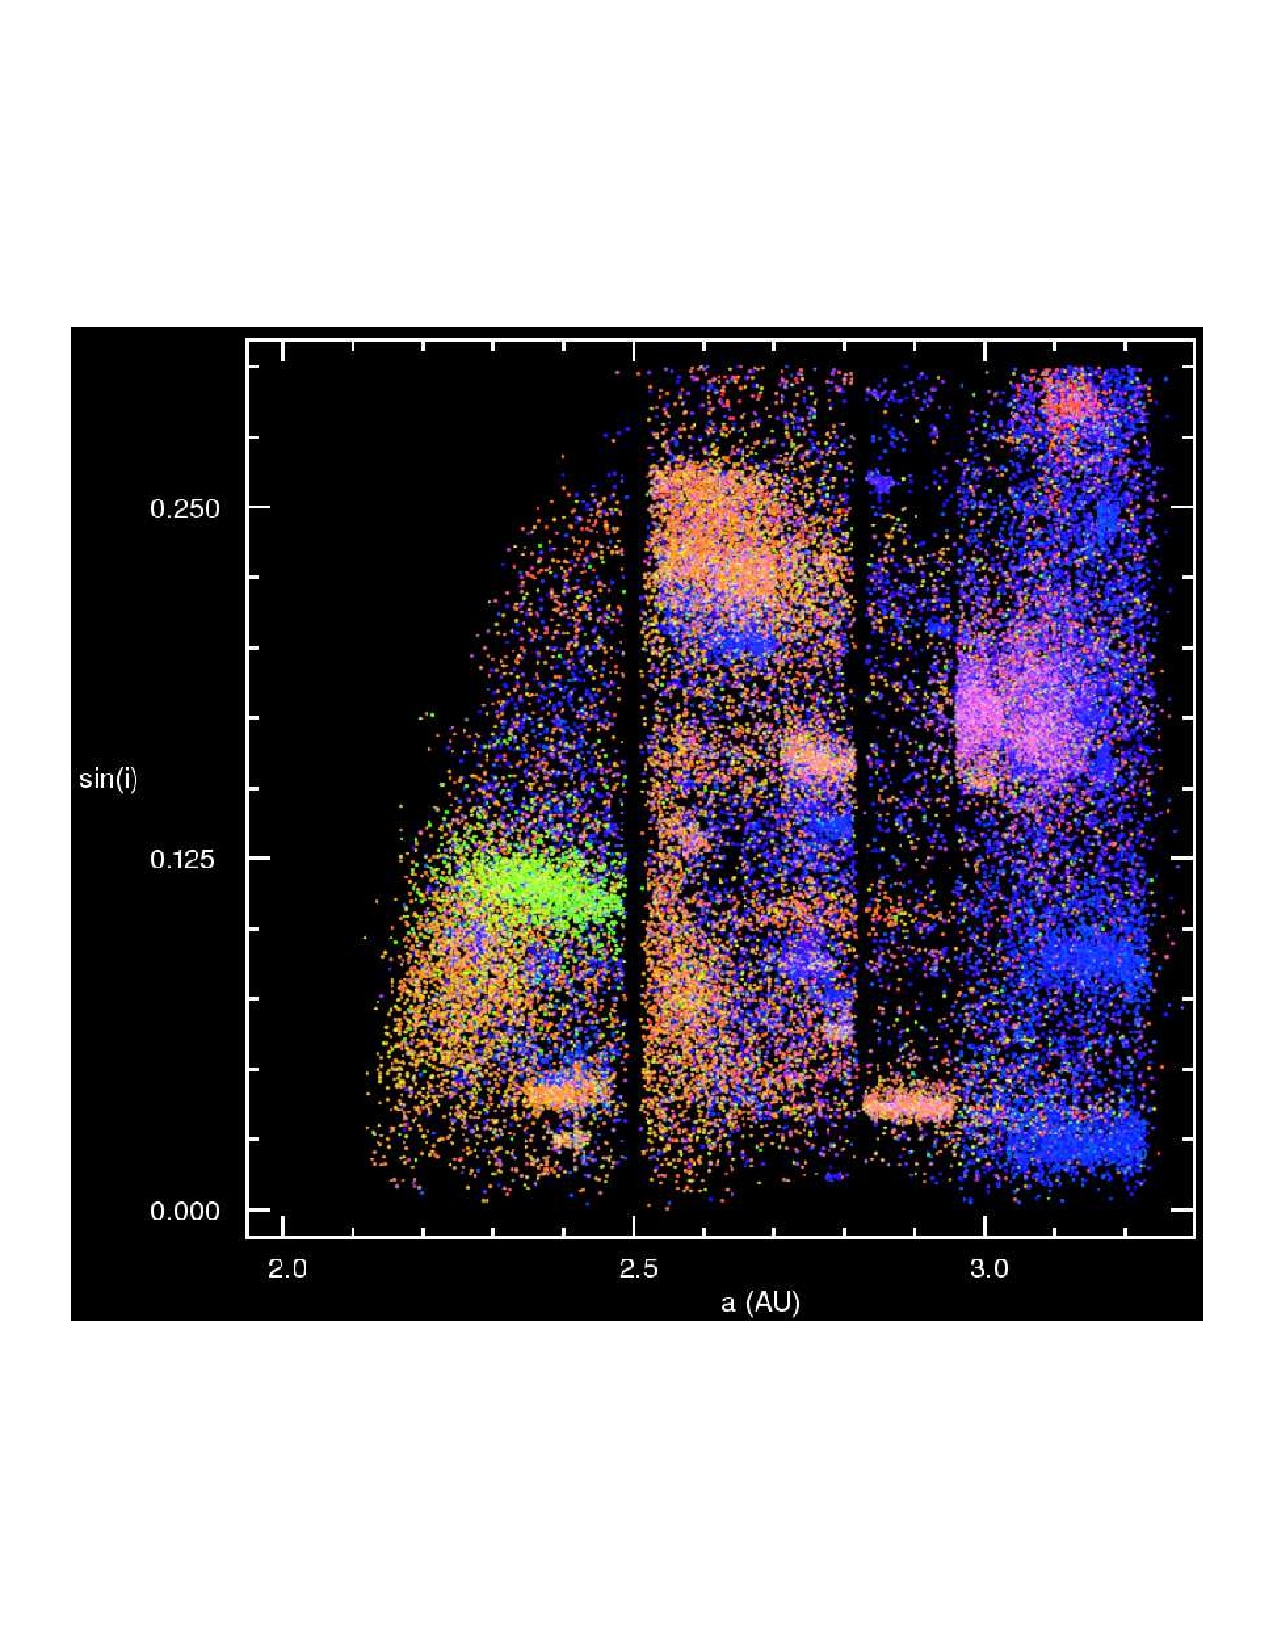
\includegraphics[width=1.0\hsize,clip]{asteroids.pdf}
\caption{An example of color-based asteroid taxonomy. The figure
shows the distribution of asteroids in the proper semi-major axis vs. $\sin(i)$
plane for 45,000 asteroids with colors measured by SDSS (Parker et al. 2008). 
The color of each dot is representative of the object's color.
Note the strong correlation between asteroid families (objects in distinct regions
of the plane) and colors. There are
at least five different taxonomic types distinguishable with SDSS measurements;
LSST color measurements of asteroids will be more than twice as accurate
and will increase the number of objects by $\sim$2 orders of magnitude.} 
\label{Fig:asteroids}
\end{figure}

\begin{figure}
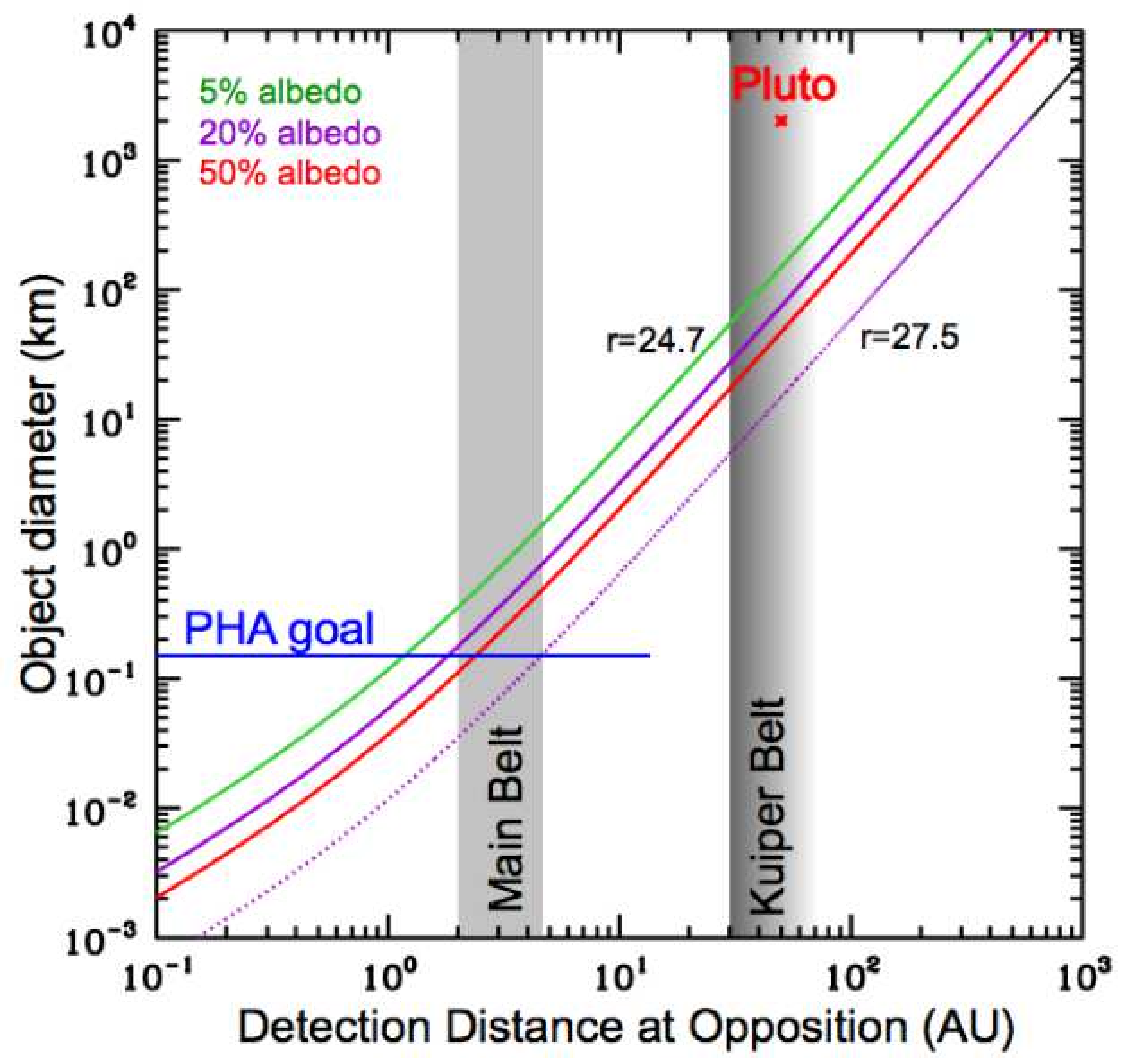
\includegraphics[width=1.0\hsize,clip]{Af9.pdf}
\caption{The LSST detection limits for distant solar system objects.
Moving objects with diameters as small as 100m in the main asteroid belt and 
100km in the Kuiper Belt (TNOs) will be detected. Specialized deeper observations 
(see \S~\ref{Sec:minisurveys}) will detect TNOs as small as 10 km. Adapted from 
Jones et al. (2007).} 
\label{Fig:Af9}
\end{figure}


\subsection{ Exploring the Transient Optical Sky }


\begin{figure}
\hskip -0.1in
\vskip -0.1in
%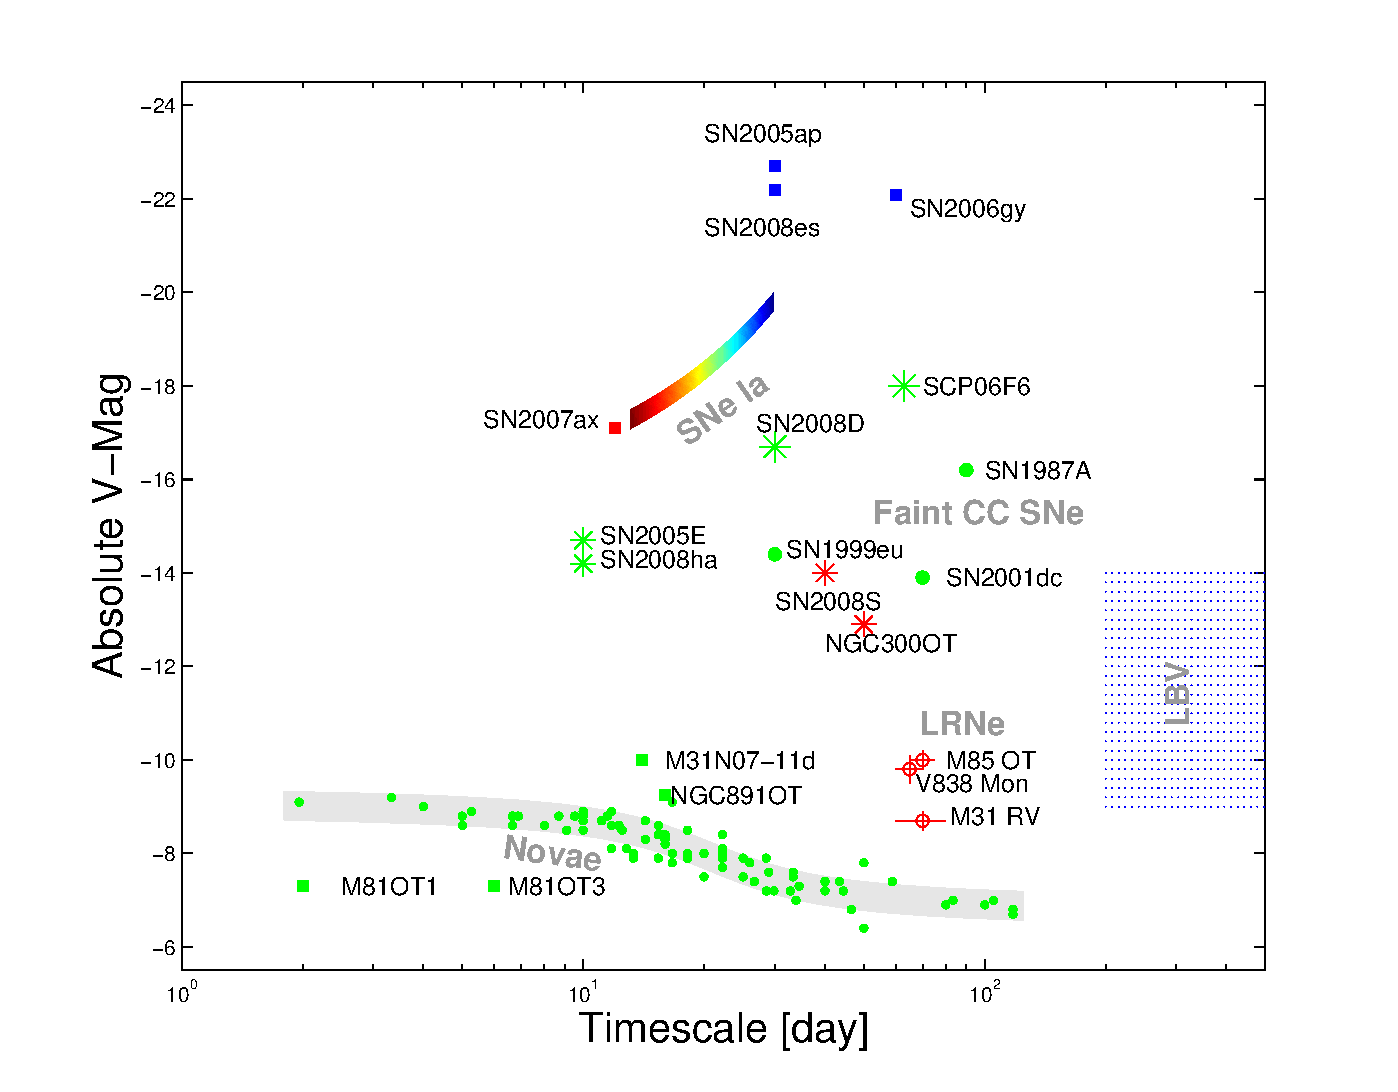
\includegraphics[width=1.1\hsize,clip]{shri2.pdf}
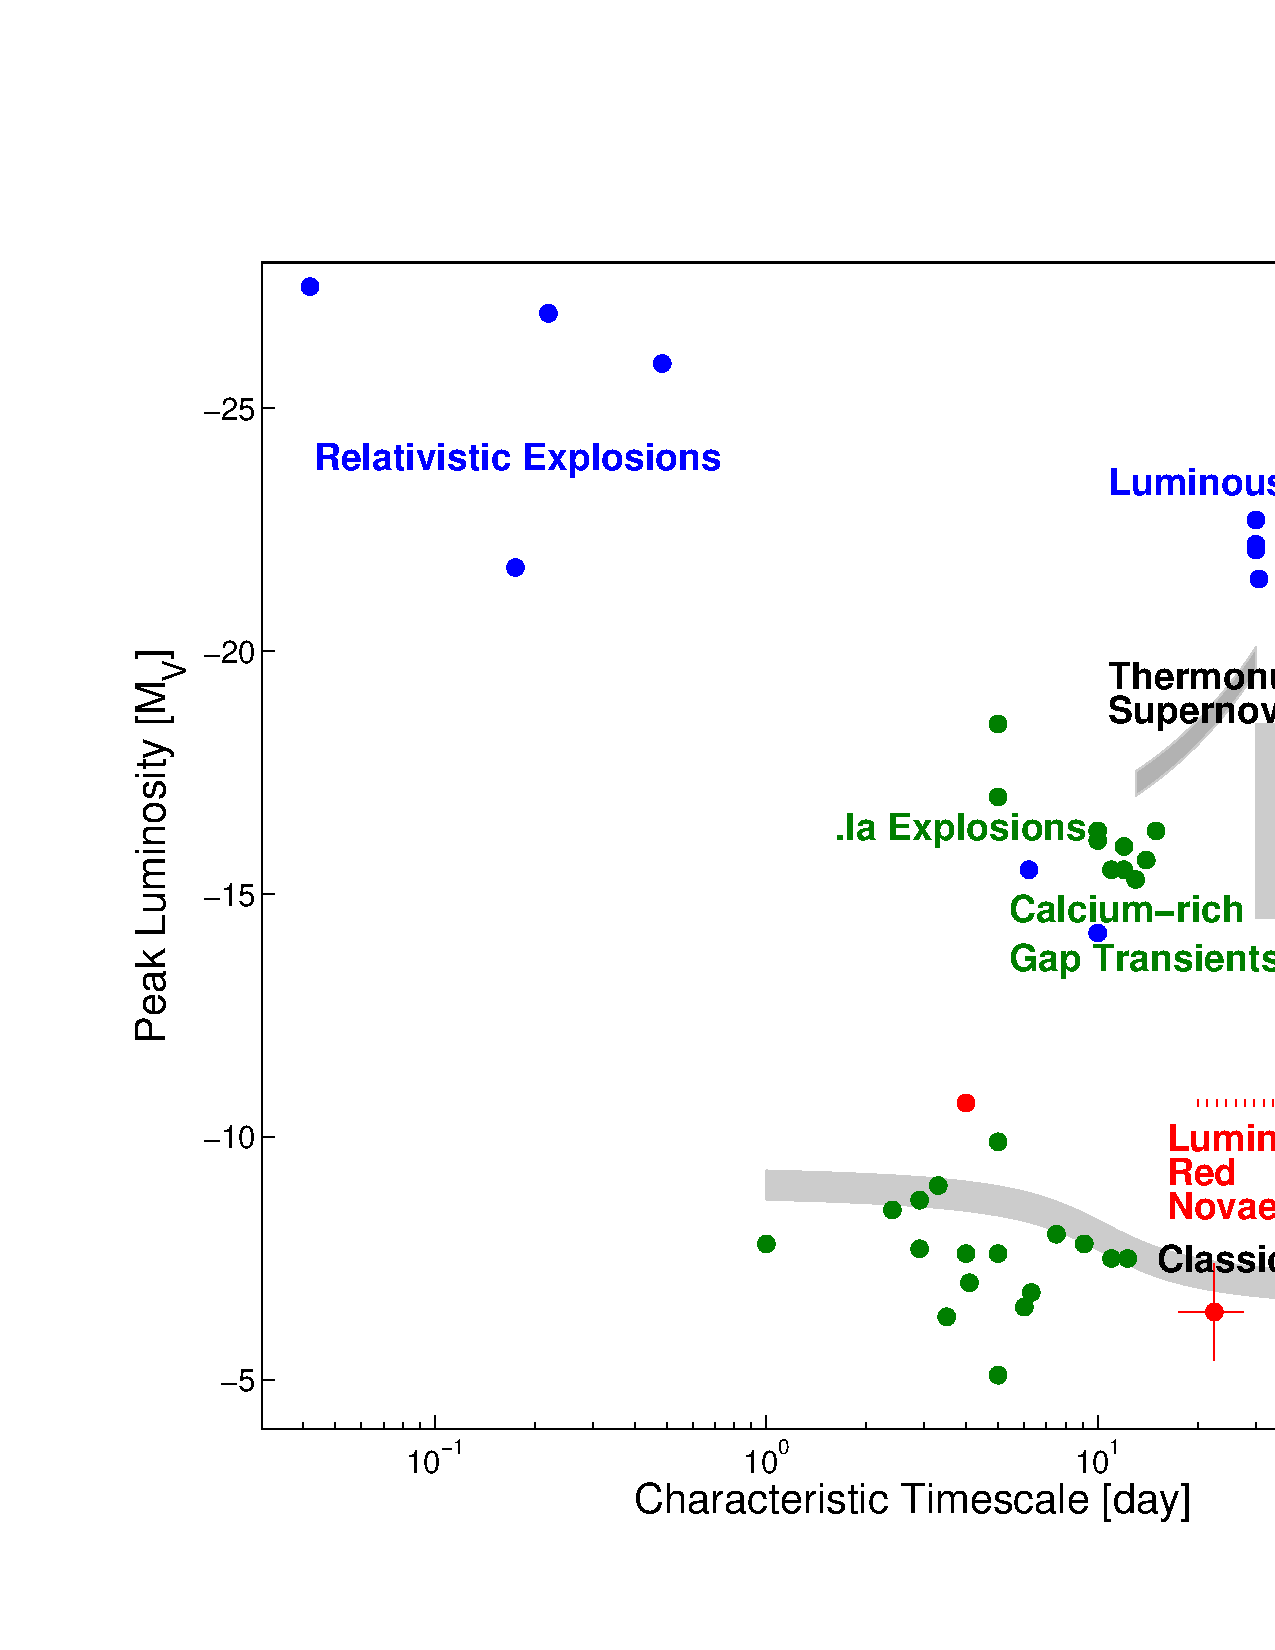
\includegraphics[width=1.0\hsize,clip]{taumv.pdf}
%\vskip -0.1in
\caption{The phase space of cosmic explosive and eruptive transients as
represented by their absolute $V$ band peak brightness and the 
event timescale (adapted from Kulkarni et al. 2007). LSST will open up large 
regions of this phase space for systematic exploration by extending
time-volume space 1000 times over existing surveys.} 
\label{Fig:shri}
\end{figure}



Time domain science will greatly benefit from LSST's unique capability to simultaneously
provide large area coverage, dense temporal coverage, accurate color information,
good image quality, and rapid data reduction and classification. Since LSST extends 
time-volume space a thousand times over current surveys (e.g., Morokuma et al. 2008), 
the most interesting science may well be the discovery of new classes of objects.  
There are many projects that LSST data products will enable:

\begin{itemize}
\item Detection and measurement of gamma-ray burst afterglows and transients 
      (e.g., Zhang \& M\'{e}sz\'{a}ros 2004) to high redshift ($\sim$7.5).
\item Studies of optical bursters (those varying faster than 1 mag hr$^{-1}$) to $r\sim25$ mag. 
\item Gravitational micro-lensing in the Local Group and beyond (de Jong, Kuijken \& H\'{e}raudeau 2008).
\item Studies of known and unusual SN populations and parametrization of their light curves 
         (e.g., Hoeflich, Wheeler \& Thielemann 1998; Howell et al. 2007).
\item Studies of dwarf novae, including their use as probes of stellar populations and 
      structure in the Local Group (Neill \& Shara 2005).
\item A deep search for new populations of novae and supernova progenitors 
      (Kulkarni et al. 2007; see Fig.\ref{Fig:shri}). 
\item Search for stellar tidal disruptions by nuclear supermassive black
       holes (Evans \& Kochanek 1989; Gezari et al. 2008), \B{as well as binary supermassive black holes 
      in the in-spiral phase (e.g., Cuadra et al. 2009).}
\item A study of quasar variability using 1-2\% accurate, multicolor light
      curves for $\sim$2 million quasars, leading to constraints on the accretion physics
      and nuclear environments (de Vries, Becker \& White 2003; Vanden Berk et al. 2004, MacLeod 
      et al. 2010). Relations between quasar variability properties and luminosity, redshift, 
      rest-frame wavelength, time scale, color, radio-jet emission, black-hole 
      mass, and Eddington-normalized luminosity will be defined with massive
      statistics. Microlensing events will also be monitored in the $\sim$4000 gravitationally-lensed 
      quasars discovered by LSST and used to measure the spatial structure of quasar accretion disks.
\item The superb continuum light curves of AGN will enable economical ``piggyback" 
      reverberation-mapping efforts using emission lines. These results 
      will greatly broaden the luminosity-redshift plane of reverberation-mapped AGNs
      with black-hole mass estimates. For LSST data alone, the inter-band continuum lags 
      will provide useful structural information. 
\item LSST data will allow good constraints on AGN lifetimes, or at least the timescales over which 
         they make distinct accretion-state transitions, due to large sample
         size and survey lifetime (e.g., Martini \& Schneider 2003).
\item Optical identifications for transients and variables detected at other wavelengths,
      from gamma-rays to radio, as well as by means other than electro-magnetic
      radiation (e.g., LIGO\footnote{http://www.ligo.caltech.edu}, 
%     LISA\footnote{http://lisa.nasa.gov}, 
      ICECUBE\footnote{http://icecube.wisc.edu}).
\end{itemize}



\subsection{ Mapping the Milky Way }

The LSST will map the Galaxy in unprecedented detail, and by doing so revolutionize 
the fields of Galactic Astronomy and Near-field Cosmology. The great detail with which 
the Milky Way can be studied complements the statistical power of extra-galactic 
observations.  The overarching goal of near-field cosmology is to use spatial, kinematic, 
and chemical data sets of stars to reveal the structure and evolution history
of the Milky Way and its environment. LSST will reveal this fossil record in
great detail and provide a Rosetta Stone for extragalactic astronomy by
setting the context within which we interpret these broader data
sets. Moreover, by providing a census of faint satellites and stellar streams
in the halo, this map will offer a unique means to constrain the 
particle nature of dark matter because candidate supersymmetric particle dark
matter models predict different mass clustering on small scales, with a
corresponding range of mass profiles in low-mass systems. 


The LSST will produce a massive and exquisitely accurate photometric and astrometric data 
set for about 10 billion Milky Way stars. The coverage of the Galactic plane
will yield data for numerous star-forming regions, and the $y$ band data 
will penetrate through the interstellar dust layer. Photometric metallicity
measurements (see Figs.~\ref{Fig:FeH} and \ref{Fig:FeH3}) will be available for about 
200 million main-sequence F/G stars which will sample the halo to distances of 100 kpc 
(Ivezi\'{c} et al. 2008a). No other existing or planned survey will provide
such a powerful dataset to study the outer halo, including Gaia
which is flux limited at $r=20$, the SkyMapper (Keller et al. 2001) which is flux limited to $r=22.6$
(but will nicely complement SDSS in the Southern hemisphere), and Pan-STARRS 
which lacks the $u$ band (which is necessary for estimating metallicity). 
The LSST in its standard surveying mode will be able to detect RR Lyrae 
variables (pulsating stars and standard candles) and classical novae
(exploding stars and standard candles) at a distance of 400 kpc and hence
explore the extent and structure of our  halo out to half the distance to 
the Andromeda galaxy. Thus, the LSST will enable studies of 
the distribution of main-sequence stars beyond the presumed edge of the 
Galaxy's halo (see Fig.~\ref{Fig:halo}), of their metallicity distribution 
throughout most of the halo, and of their kinematics beyond the thick
disk/halo boundary. LSST will also obtain direct distance measurements via
trigonometric parallax below the hydrogen-burning limit for a representative 
thin-disk sample. 

In addition to the study of hydrogen burning stars, LSST will uncover the largest 
sample of stellar remnants to date. Over 97\% of all stars eventually exhaust their 
fuel and cool to become white dwarfs. Given the age of the Galactic halo, most of 
the mass in this component now resides in these remnant stars (e.g., Alcock et al. 
2000) and therefore their discovery directly constraints the Galactic mass budget.  
These large populations of disk and halo white dwarfs will provide unprecedented 
constraints on the luminosity function of these stars, which will directly yield 
independent ages for the Galactic disk and halo (e.g., through the initial-final mass 
relation, Kalirai et al. 2008).

The sky coverage of LSST naturally targets both field stars and star clusters.  
To date, no systematic survey of the stellar populations of Southern hemisphere clusters 
has been performed (e.g., such as the CFHT Open Star Cluster Survey or the WIYN Open 
Star Cluster Survey in the North; Kalirai et al. 2001; Mathieu 2000).  
Multiband imaging of these co-eval, co-spatial, and iso-metallic systems will provide 
vital insights into fundamental stellar evolution.  For example, the depth of 
LSST will enable construction of  luminosity and mass functions for nearby open clusters 
down to the hydrogen burning limit and beyond.  Variations in the initial mass function will be 
studied as a function of environment (e.g., age and metallicity).  The wide-field 
coverage will also allow us to track how the stellar populations in each cluster vary 
as a function of radius, from the core to beyond the tidal radius. Fainter remnant 
white dwarfs will be uncovered in both open and globular clusters (the nearest of which 
are all in the South), thereby providing a crucial link to the properties of the now 
evolved stars in each system. 


\begin{figure}
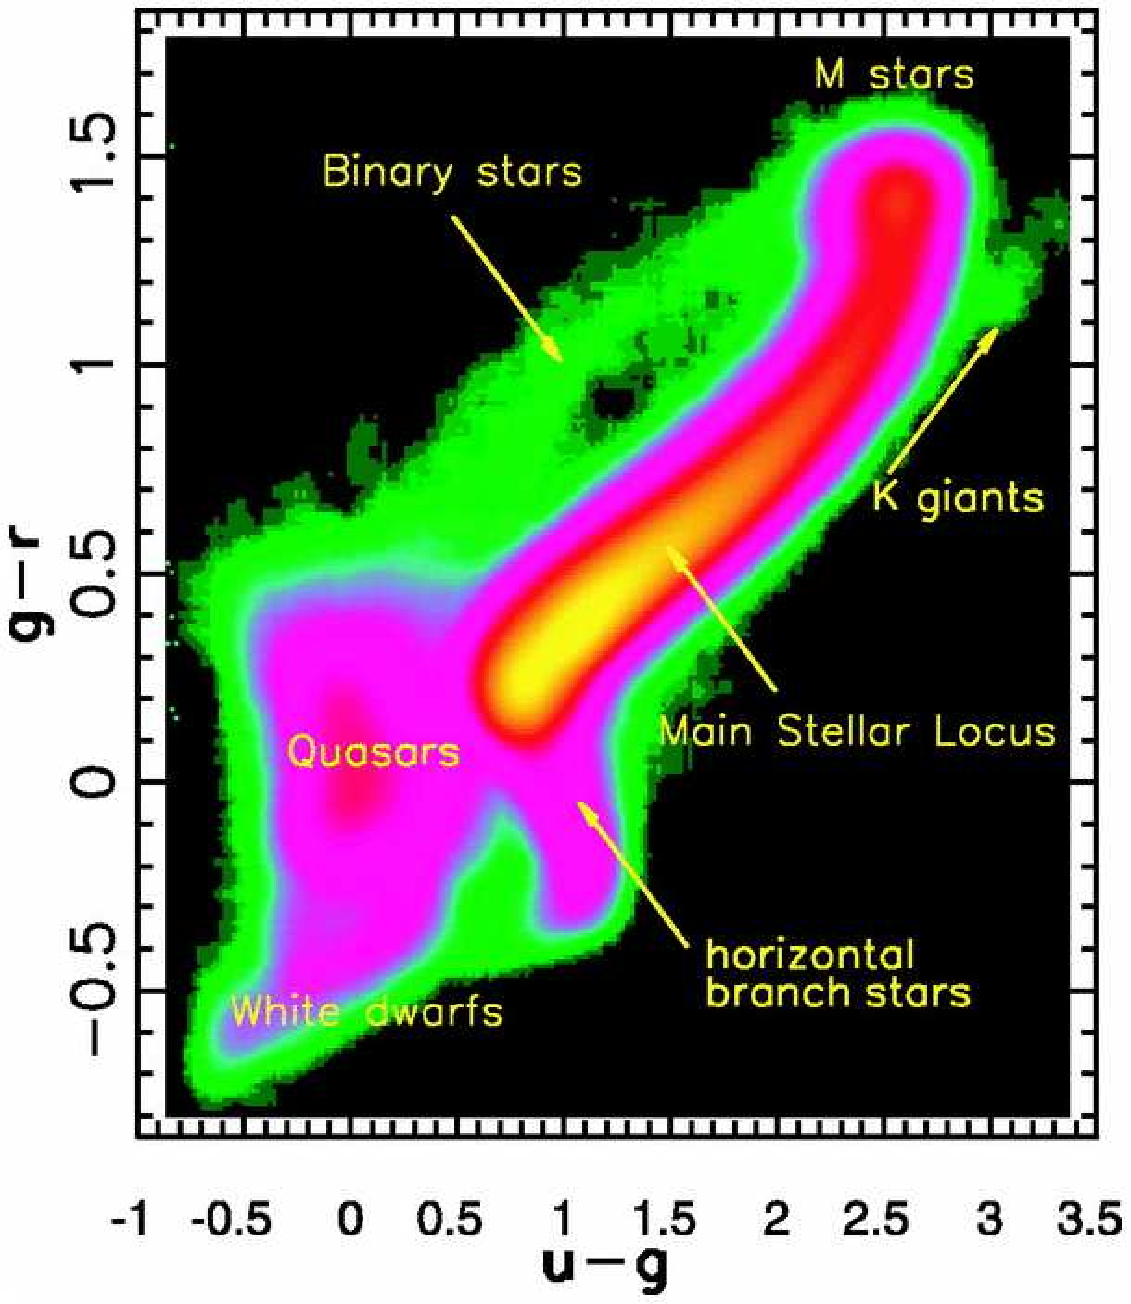
\includegraphics[width=1.0\hsize,clip]{smolcic.pdf}
\caption{The $g-r$ vs. $u-g$ color-color diagram for two million stars measured by 
SDSS (adapted from Smol\v{c}i\'{c} et al. 2004). Accurate multi-color photometry 
contains information that can be used for source classification and determination of 
detailed stellar properties such as effective temperature and metallicity. LSST will 
enable such measurements for billions of stars.} 
\label{Fig:FeH}
\end{figure}

\begin{figure}
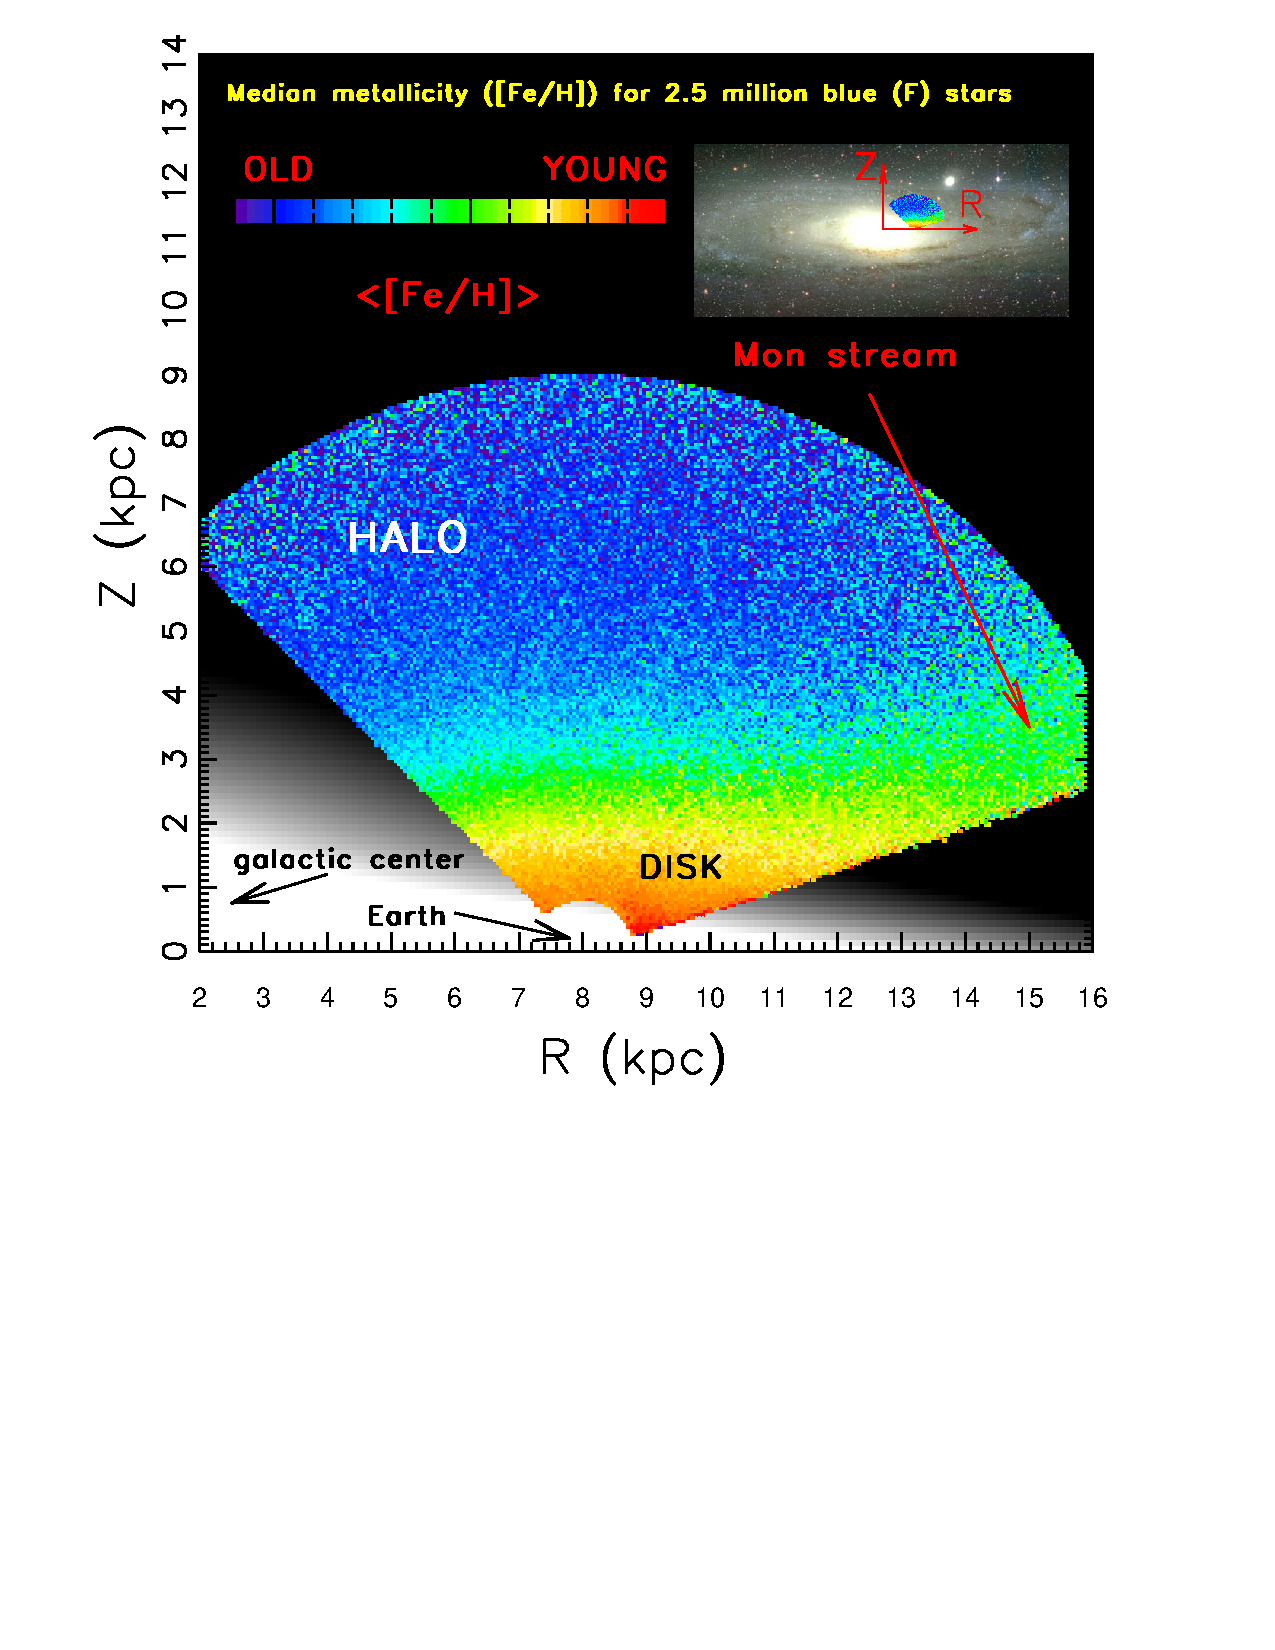
\includegraphics[width=1.0\hsize,clip]{panelsLSST.pdf}
\caption{
The median metallicity map for 2.5 million main-sequence F-type stars within 10 kpc 
from the Sun (adapted from Ivezi\'{c} et al. 2008a). The metallicity is estimated using 
$u-g$ and $g-r$ colors measured by SDSS. The position and size of the mapped 
region, relative to the rest of the Milky Way, is illustrated in the top right 
corner, where the same map is scaled and overlaid on an image of the Andromeda 
galaxy. The gradient of the median metallicity is essentially parallel
to the $Z$ axis, except in the Monoceros stream region, as marked. LSST 
will extend this map out to 100 kpc, using a sample of over 100 million 
main-sequence F stars.} 
\label{Fig:FeH3}
\end{figure}


\begin{figure}
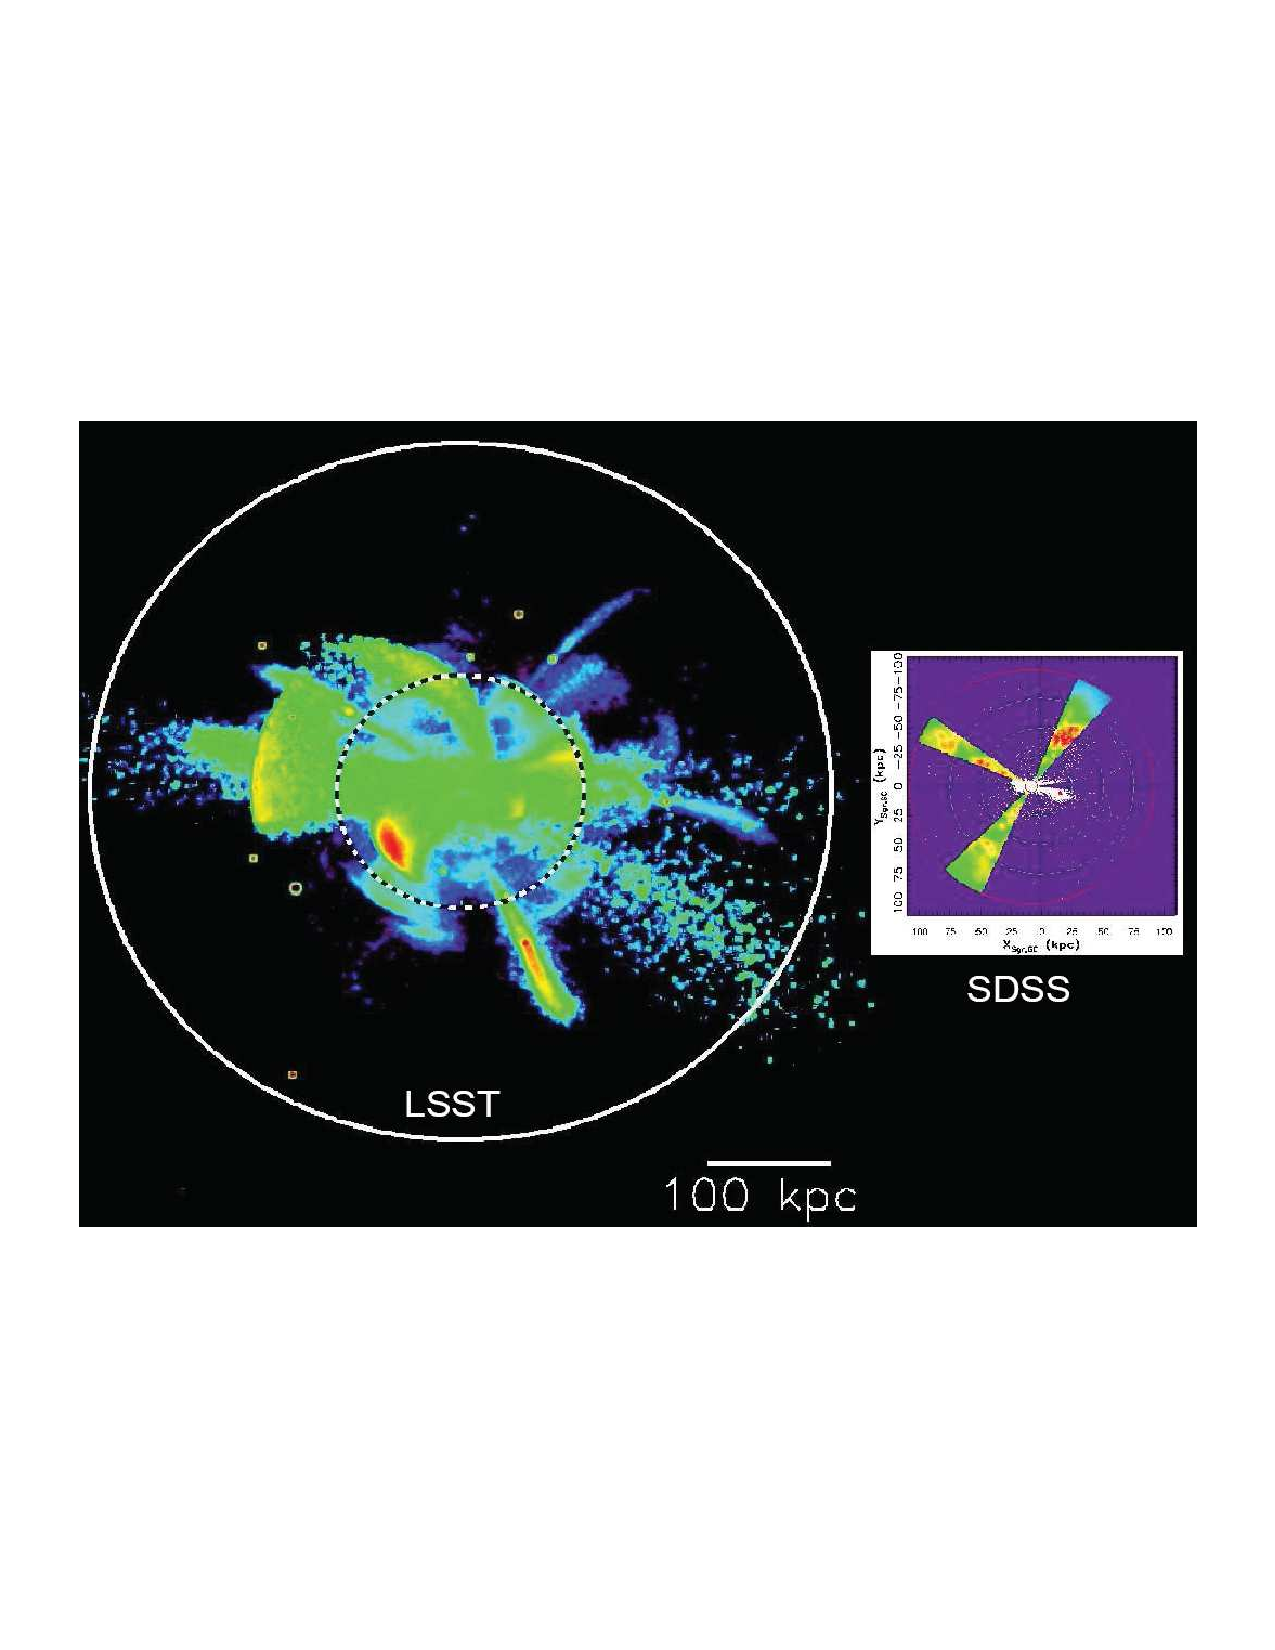
\includegraphics[width=1.0\hsize,clip]{halo.pdf}
\caption{A simulation of the outer regions of the Milky Way (left), compared to the 
current state-of-the-art data (right), shown on the same spatial scale. The data panel 
presents the number density multiplied by the cube of the Galactocentric
radius (logarithmic scale with dynamic range of 1000, from blue to red), for $\sim$1000 
SDSS RR Lyrae stars within 10$^\circ$ of the Sgr dwarf tidal stream plane (Ivezi\'{c} et 
al. 2003). The same color coding was used to visualize stellar number density for a Milky 
Way type galaxy simulation from Bullock and Johnston (2005), shown on the left. Set with 
an $\Lambda$CDM merger history, these simulations track the accretion and 
disruption of hundreds of dwarf galaxies into Milky-Way size halos. With LSST, RR Lyrae 
stars will be found beyond the presumed Milky Way tidal radius ($\sim$300 kpc, white circle), 
and the much more numerous main-sequence stars will trace the structure out to 100 kpc 
(dashed circle), with similar fidelity as shown in Figure~\ref{Fig:FeH3}. The latter 
distance range can now be probed only using RR Lyrae stars and other rare 
non-main-sequence stars.} 
\label{Fig:halo}
\end{figure}
 

\begin{figure}
\vskip -1in
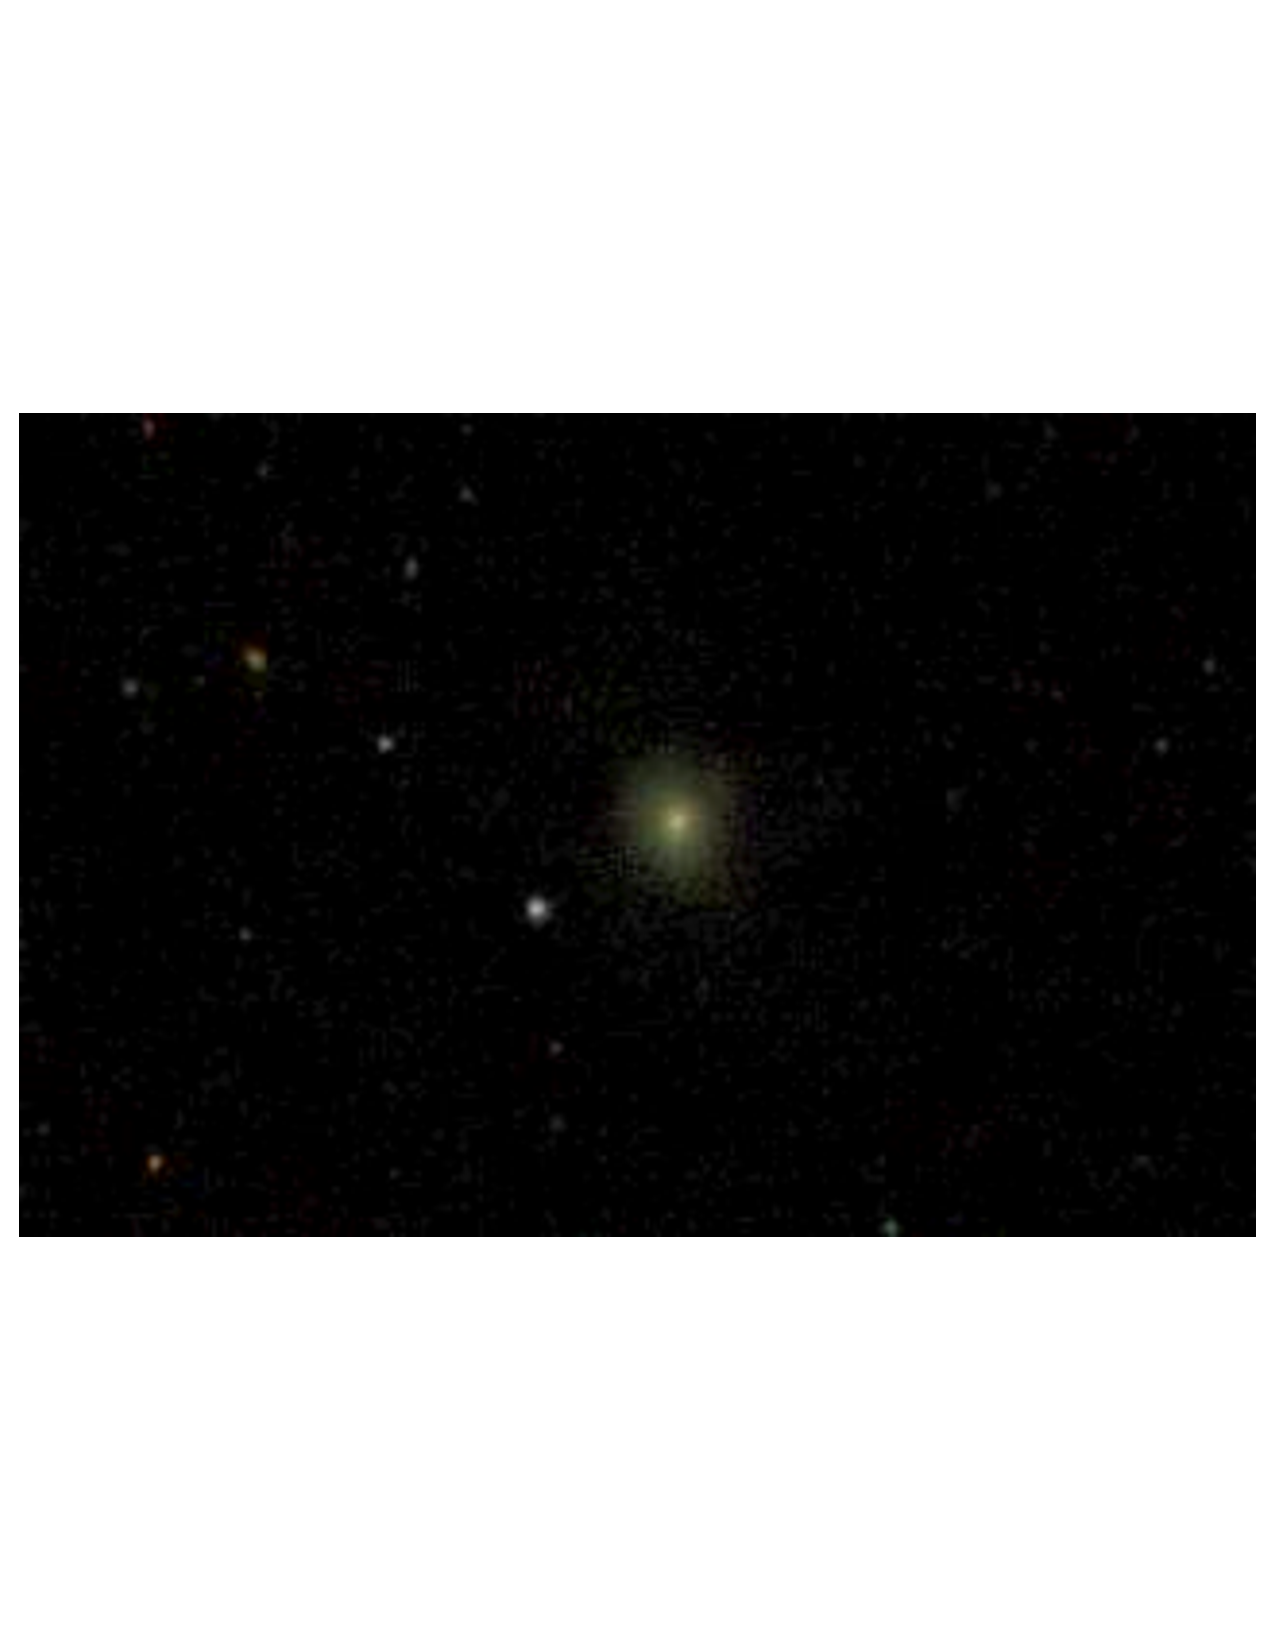
\includegraphics[width=1.0\hsize,clip]{musycSDSS.pdf}
\vskip -1.9in
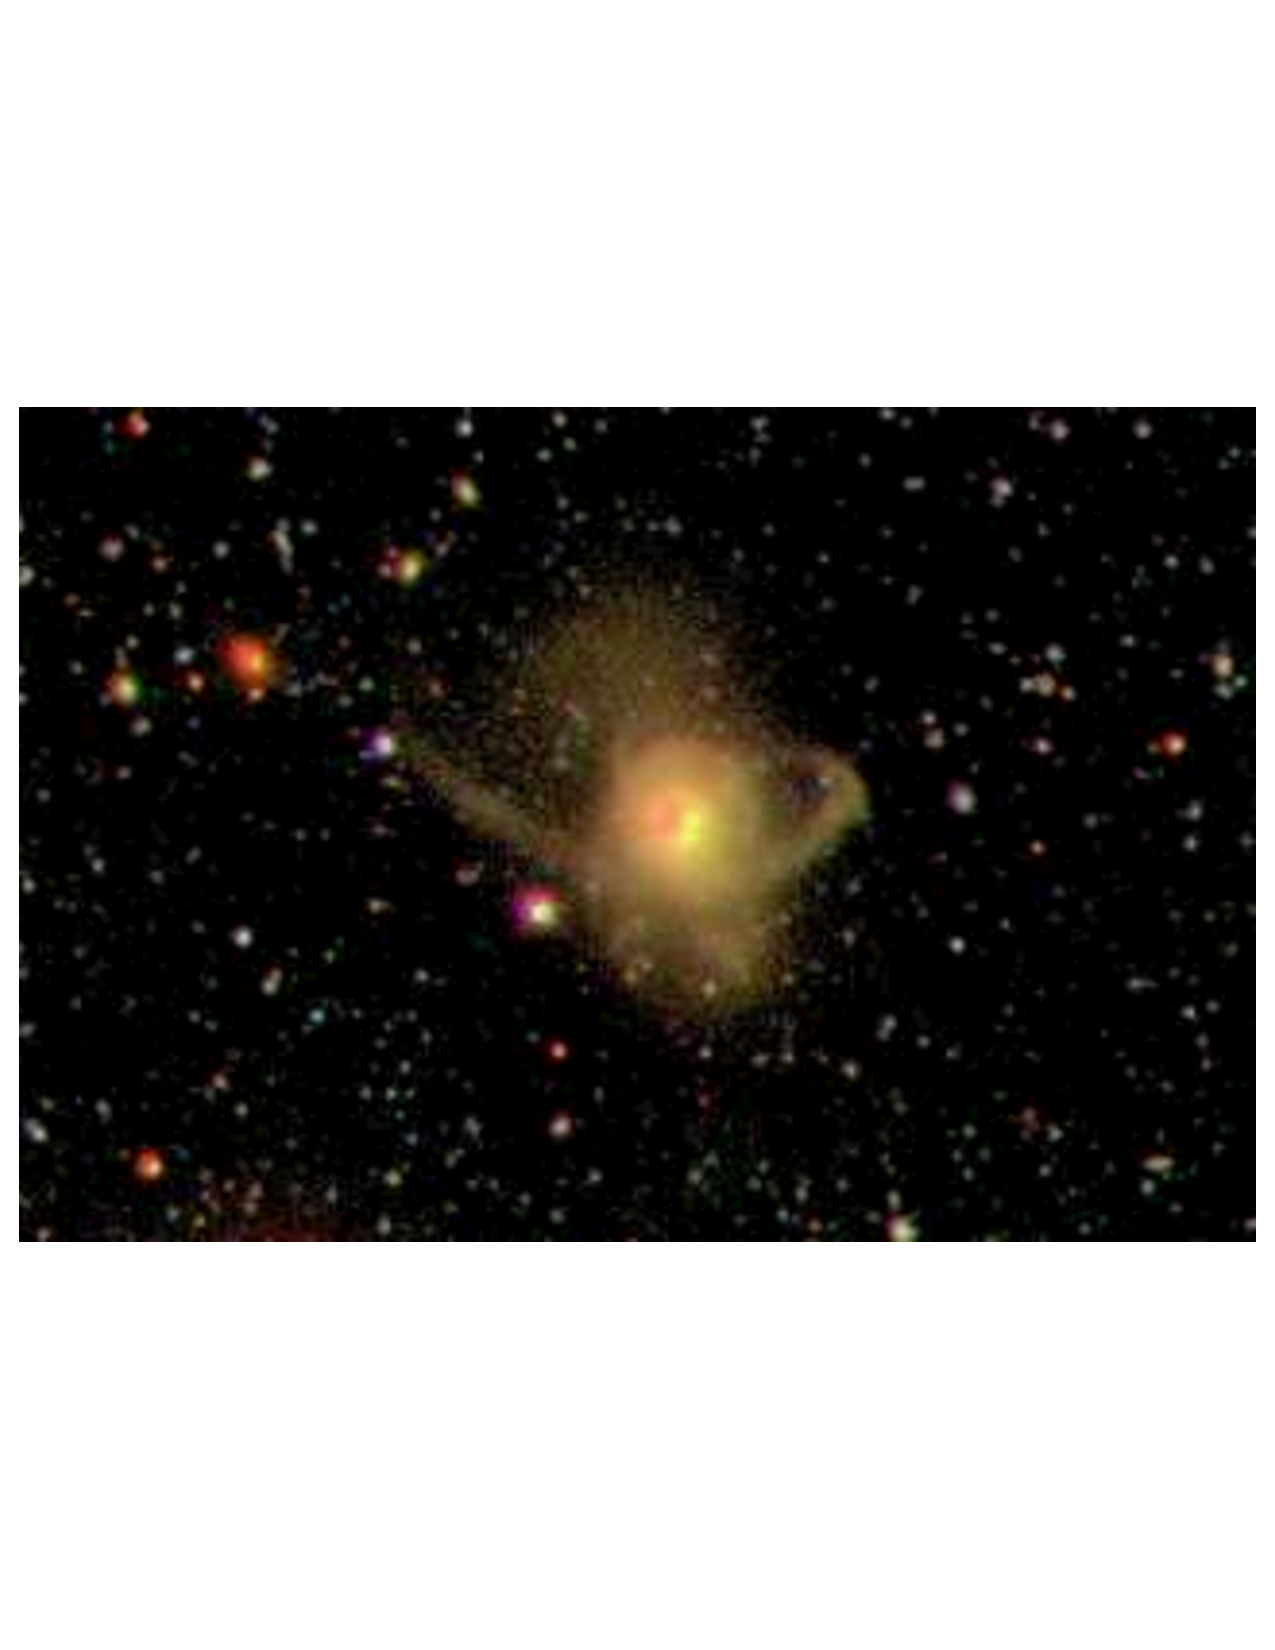
\includegraphics[width=1.0\hsize,clip]{musyc.pdf}
\vskip -1in
\caption{
A comparison of an SDSS image (2$\times$4 arcmin$^2$ $gri$ composite) showing a typical galaxy at 
a redshift of $\sim$0.1 (top) with a similar $BVR$ composite image of the same field obtained by the MUSYC survey (bottom; 
Gawiser et al. 2006). The MUSYC image is about 4 mag deeper than the SDSS image (and about 1 mag less deep 
than anticipated LSST 10-year coadded image). Note the rich surface brightness structure seen in the MUSYC 
image that is undetectable in the SDSS image.} 
\label{Fig:musyc}
\end{figure}


In summary, the LSST data will revolutionize studies of the Milky Way and the entire
Local Group (Saha et al. 2007). We list a few specific Galactic science programs that 
LSST will enable: 

\begin{itemize} 
\item High-resolution studies of the distribution of stars in the outer halo
      in the six-dimensional space spanned by position, metallicity and proper
      motions (e.g., Girard et al. 2006; Bell et al. 2008; Juri\'{c} et al. 2008;
      Ivezi\'{c} et al. 2008a; Bond et al. 2010).
\item The faintest ever search for halo streams, and galaxy satellites and intergalactic stars 
      over much of the Local Group (e.g., Grillmair 2006ab; Ibata et al. 2007; Walsh, 
      Jerjen \& Willman 2007; Belokurov et al. 2007a).
\item Deep and highly accurate color-magnitude diagrams for over half of the known 
      globular clusters, including tangential velocities from proper motion 
      measurements (Casetti-Dinescu et al. 2007; Clem, VandenBerg \& Stetson 2008). 
\item Mapping the metallicity, kinematics and spatial profile of the Sgr dwarf tidal 
      stream (e.g., Ibata et al. 2001; Majewski et al. 2003; Law, Johnston \& Majewski 2005)
       and the Magellanic stream (Zaritsky et al. 2004). 
\item Studies of the clumpiness of the gravitational potential in the Galaxy using 
      fragile wide-angle binaries selected with the aid of trigonometric and 
      photometric parallaxes, and common proper motion (e.g., Yoo, Chanam\'{e} \& Gould 2004).
\item Detailed studies of variable star populations; 2\% or better accurate 
      multicolor light curves will be available for a sample of at least 50 
      million variable stars (Sesar et al. 2007), enabling studies of
      cataclysmic variables, eclipsing binary systems, and rare types of variables.
\item Discovery of rare and faint high proper motion objects: probing the
      faint end of the stellar mass function (Lepine 2008), and searching for 
      free-floating planet candidates (Lucas \& Roche 2000).
\item Direct measurement of the faint end of the stellar luminosity function 
      using trigonometric parallaxes (Gratton et al. 1997) and a complete census of the 
      solar neighborhood to a distance of 100 pc based on trigonometric parallax measurements 
      for objects as faint as $M_r=17$. For example, LSST will deliver 10\% or
      better distances for a sample of about 2,500 stars with
      18$<M_r<$19. There are only a handful of such stars known today 
      (Gaia will detect fewer than 100). 
\item The separation of halo M sub-dwarfs from disk M dwarfs, using 
      the $z-y$ color which is sensitive to their rich molecular band structure
      (West et al. 2004; Lepine \& Scholz 2008).
\item \B{Studies of white dwarfs using samples of several million objects, 
    including the determination of the halo white dwarf luminosity function  
     (SciBook Ch.~6). }
\item \B{Measurements of physical properties of stars using large samples  
        of eclipsing binary stars (SciBook Ch.~6). }
\item Planetary transits: the data set may include a mini survey of 600
      deg$^2$ of sky which will collect about 40 hour-long sequences of 200 
      observations each over a 4-month period (see \S~\ref{Sec:minisurveys}). 
      There would be an additional 800 observations over 10 years of these
      same fields as part of the main survey. With about 10 million or more stars 
      in the sample (depending on where the fields are placed), this would
      provide excellent base material to study the planet frequency as a
      function of stellar type, metallicity, and distance from the Galactic plane
      (e.g., Charbonneau et al. 2000; Konacki et al. 2003).
\item A census of AGB stars in the Galaxy by searching for 
      resolved envelopes and optical identifications of IR counterparts (e.g., from 
      IRAS and Spitzer surveys), and by using long-term variability and color 
      selection (Ivezi\'{c} 2007c).
\item A complete census of faint populations in nearby star forming regions using 
      color and variability selection (e.g., Briceno et al. 2005). 
\item High-resolution three-dimensional studies of interstellar dust using 5-color 
      SEDs of main sequence stars (McGehee 2004; Meyer et al. 2005). 
\end{itemize} 

\begin{figure}
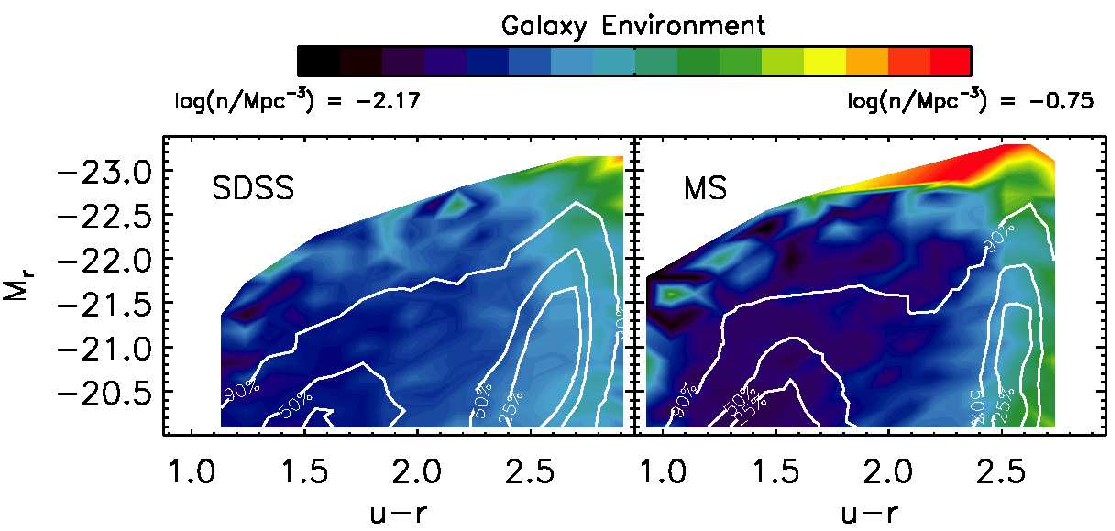
\includegraphics[width=1.0\hsize,clip]{cowan.pdf}
\caption{A comparison of the distribution of galaxies in  
luminosity--color--density space measured by SDSS (left) and a model based
on the Millennium simulation (right). The linearly-spaced contours outline
the distribution of volume-limited sample of galaxies in the plotted diagram, and
the color-coded background shows the median environmental density (computed
using the ten nearest neighbors) for galaxies
with the corresponding luminosity and color. Such multi-variate distributions
encode rich information about formation and evolution of galaxies. Galaxies 
detected by SDSS are representative of the low-redshift Universe (the median 
redshift is $\sim$0.1). The LSST will enable such studies as a function of 
redshift, to $z\sim$2. Adapted from Cowan \& Ivezi\'{c} 
(2008).} 
\label{Fig:cowan}
\end{figure}


\begin{figure}
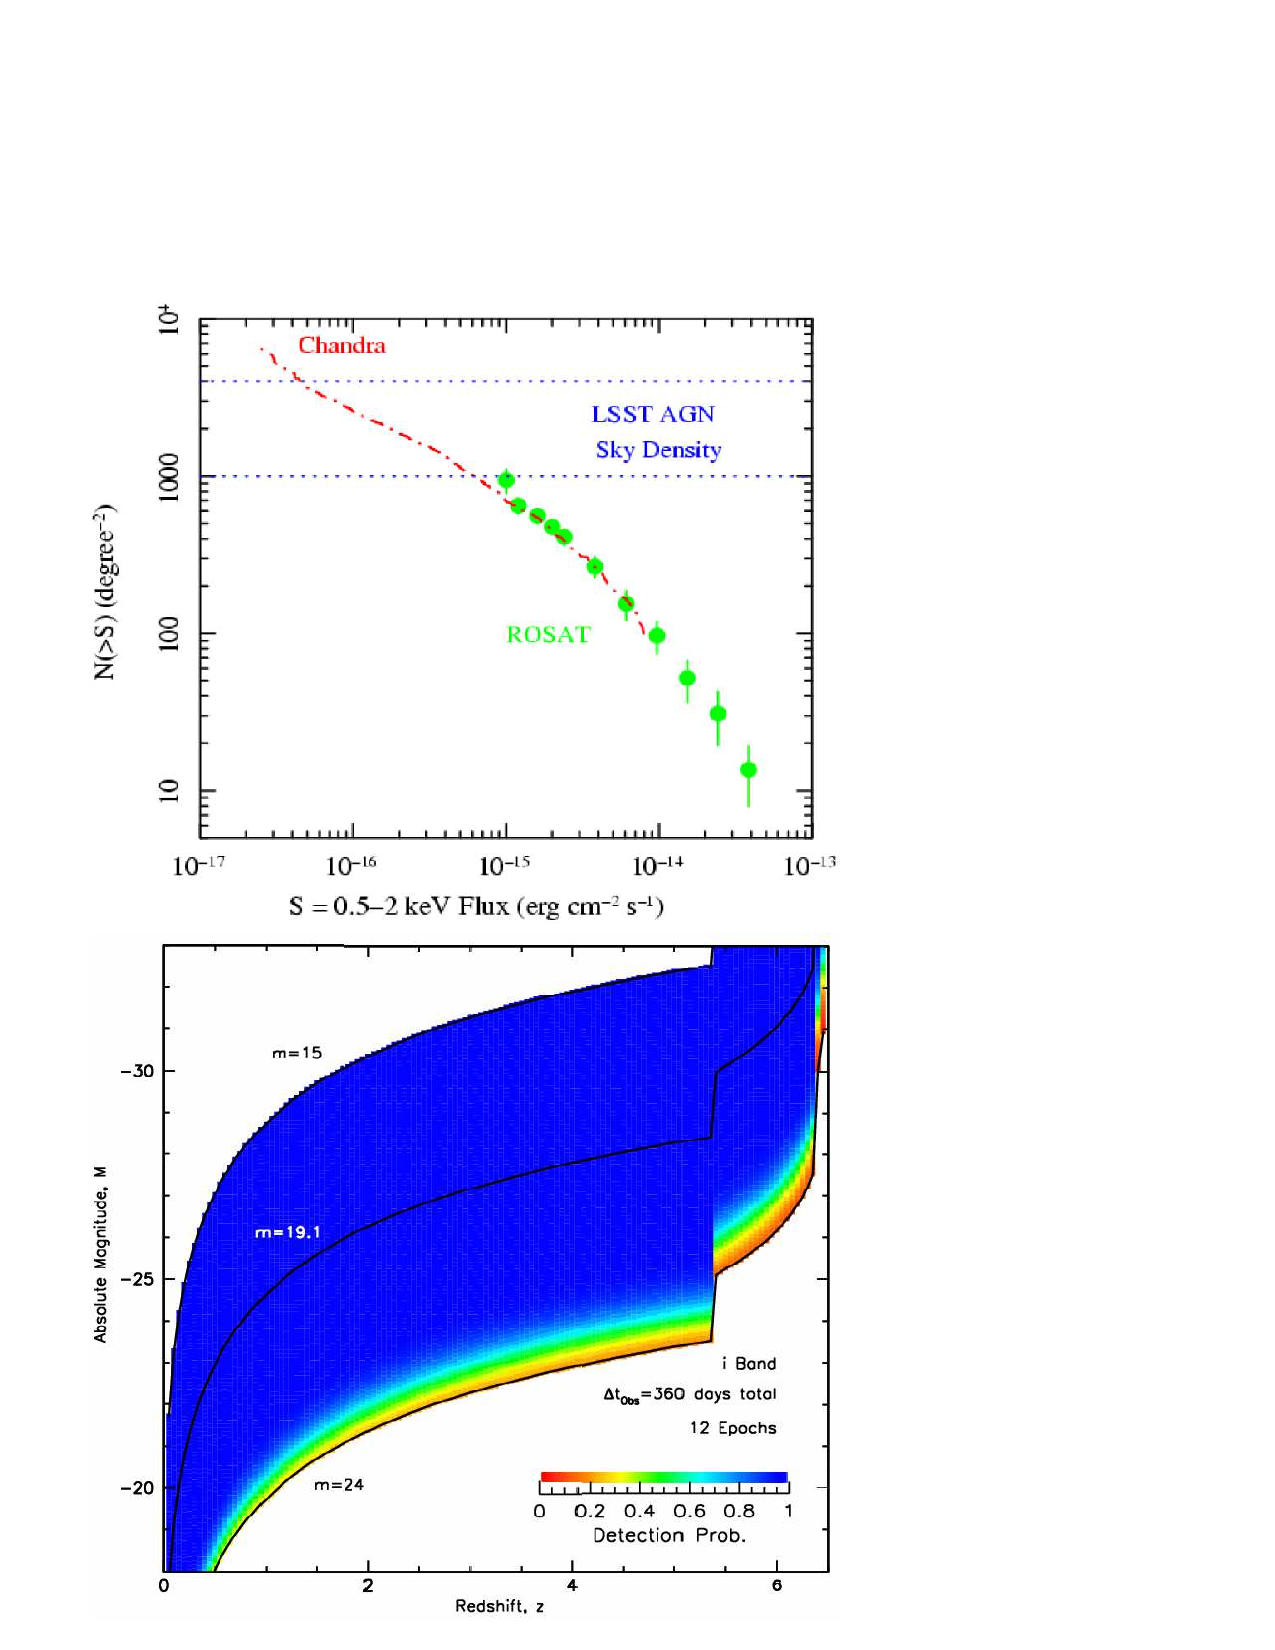
\includegraphics[width=1.0\hsize,clip]{panels3.pdf}
\caption{The LSST will deliver AGN sky densities of 1000-4000 deg$^{-2}$, which is 
competitive with the deepest pencil-beam surveys to date, such as the Chandra
Deep Fields (top panel). The total LSST AGN yield, selected using colors and
variability, should be well over 10 million objects. 
The bottom panel shows the expected distribution of these objects in the 
absolute magnitude vs. redshift plane, color-coded by the probability for
an object to be
detected as variable after 1 year of observations. Note that quasars will
be detected to their formal luminosity cutoff ($M< -23$) even at redshifts
of $\sim$5. Adapted from Brandt et al. (2007).} 
\label{Fig:panels3}
\end{figure}


\subsection{  Additional Science Projects}

The experience with any large survey (e.g., SDSS, 2MASS, GALEX, to name but a 
few) is that much of their most interesting science is often unrelated to 
the main science drivers, and is often unanticipated at the time the survey is 
designed. LSST will enable even more diverse science than encompassed by the 
four themes that drive the system design. We list a few anticipated major 
programs.

\begin{itemize}
\item Detailed studies of galaxy formation and evolution using their distribution in 
luminosity-color-morphology space as a function of redshift. For example, LSST will 
enable studies of the rest-frame UV emission, similar to those based on GALEX data 
for local galaxies, to a redshift of $\sim$2. These studies project onto many axes:
\begin{itemize}
  \item the evolution of the galaxy luminosity function with redshift, as a function of 
        morphology and color;
  \item the evolution of the galaxy color distribution over a wide range of rest-frame 
        wavelengths, and as a function of luminosity and morphology; 
  \item bulge-disk decomposition, as a function of luminosity and color, over 
        a large redshift range; 
  \item detailed distribution of satellite galaxies in luminosity-color-morphology space 
        as a function of luminosity, color, and morphology of the primary galaxy; 
  \item correlations of luminosity, color and morphology with local environment, and
        as a function of redshift (see  Figs.~\ref{Fig:musyc} and \ref{Fig:cowan});
  \item the properties of galaxy groups as a function of cosmic time.
\end{itemize}
\item AGN census to very faint luminosity and large redshift limit, yielding
      at least 10 million objects (see Fig.~\ref{Fig:panels3}). By reaching substantially further 
      down the AGN luminosity function over a very large solid angle, LSST data 
      will test evolutionary cosmic downsizing scenarios, and lead 
      to a much clearer understanding of black-hole growth during the first Gyr. For
      example, LSST should discover $\sim$1000 AGNs at $z\sim6-7.5$,
      representing a dramatic increase over the present samples 
      (Brandt et al. 2007, see also LSST Science Book).
\item The first wide field survey of ultra low surface brightness galaxies, with 
      photometric redshift information. The currently available samples are highly
      incomplete, especially in the Southern Hemisphere (see Fig.~7 in Belokurov et al. 2007a). 
\item Search for strong gravitational lenses to a faint surface brightness limit (e.g., 
      Bartelmann et al. 1998; Tyson, Kochanski \& Dell'Antonio 1998; Belokurov et al. 2007b).
\item Multi-wavelength studies of faint optical sources using gamma-ray, X-ray, IR and
      radio data: \B{LSST will synergistically add value to archives of other observatories.}
      For example, the SDSS detected only 1/3 of all 20cm FIRST sources 
      (Becker et al. 1995) because it was too shallow by $\sim$4 mag for a complete 
      optical identification. 
\end{itemize}


\subsubsection{  Synergy with other projects }

LSST will not operate in isolation and will greatly benefit from other precursor and coeval 
data at a variety of wavelengths, depths, and timescales. For example, most of the Celestial 
Sphere will be covered to a limit several magnitudes fainter than LSST saturation 
($r\sim16$), first by the combination of SDSS, PS1 and SkyMapper (Keller et al. 2001), 
and then by the Gaia survey. The SkyMapper survey will obtain imaging data in the southern
sky to similar depths as SDSS, the Pan-STARRS surveys will provide multi-epoch data deeper 
than SDSS in the northern sky, and the Dark Energy Survey (Flaugher 2006) will scan 
$\sim$5000 deg$^2$ to similar depth as Pan-STARRS in the southern sky. Despite the lack of 
the $u$ band data and a depth about a magnitude shallower, the Pan-STARRS surveys
will represent a valuable complement to LSST in providing North sky coverage to a limit 
fainter than that of SDSS and SkyMapper. LSST and Gaia will 
be complementary datasets for studying the Milky Way in the multi-dimensional space of 
three-dimensional positions, proper motions and 
metallicity. The Gaia survey will provide calibration checks at the bright end for proper 
motions and trigonometric parallax measurements by LSST, and LSST will extend the 
Gaia survey by four magnitudes. The LSST data stream will invigorate subsequent 
investigations by numerous other telescopes that will provide 
additional temporal, spectral and spatial resolution coverage. 

LSST will provide a crucial complementary capability to space 
experiments operating in other bands, such as the planned 
%Black Hole Finder Einstein Probe 
NuSTAR Mission\footnote{http://www.nustar.caltech.edu/}, and the already successful {\it Fermi} 
Gamma-ray Space Telescope (e.g., Atwood et al. 2010) which plausibly will be continuing its high 
energy time-domain survey of the sky contemporaneously with LSST. 
%The Laser Interferometer Space Antenna (LISA) and the 
The Laser Interferometer Gravitational 
Wave Observatory (LIGO) may detect ultracompact binaries and black hole mergers through the 
gravitational wave outburst that should be emitted during the final stages of such events. 
LSST has the potential to measure the electromagnetic signal that accompanies the gravitational wave emission, 
thereby providing an accurate position on the sky for the system, which is 
crucial for subsequent observations. LSST will also add new value to the archives for 
billion-dollar class space missions such as Chandra, XMM-Newton, Spitzer,
etc., because deep optical multi-color data will enable 
massive photometric  studies of sources from these missions;
any areas of the sky --whether by design or by serendipity --in which past, present, or future 
multiwavelength surveys overlap with LSST sky coverage, will be further promoted by LSST 
investigations to ``optical plus multiwavelength Selected Areas''.   
Last but not least, the huge samples of various astronomical source
populations will yield extremely rare objects for investigations by powerful
facilities such as JWST (Gardner et al. 2006) and GSMT (Kan \& Antebi 2003).

In summary, the diversity of science enabled by LSST will be 
unparalleled, extending from the physics of gravity and the
early Universe to the properties of ``killer'' asteroids. While
there are other projects that aim to address some of the same
science goals, no other project matches this diversity and 
LSST's potential impact on society in general. 


\section{   COMMUNITY INVOLVEMENT   }
\label{Sec:community}

LSST has been conceived as a public facility: the database that it will
produce, and the associated object catalogs that are generated from that
database, will be made available to the \B{U.S. and Chilean} scientific communities,
and to the public at large, with no proprietary period. We are working with foreign partners 
to make LSST data products available worldwide. The LSST data management 
system will provide user-friendly tools to access this database and to support
user-initiated queries, run on LSST computers, either at the archive facility 
or at the data access centers. We expect that many, perhaps even the majority,
of LSST discoveries will come from research astronomers with no formal
affiliation to the project, from students, and from interested amateurs, 
intrigued by the accessibility to the Universe that this facility uniquely 
provides. For example, because of its interest in the large public data access 
of the LSST program, Google has joined the LSST team. 

The SDSS provides a good example for how the scientific 
community can be effective in working with large, publicly available
astronomical data sets. The SDSS has published a series of large incremental
data releases via a sophisticated database, roughly once per year, together with 
a paper describing the content of each data release, and extensive on-line 
documentation giving instructions on downloading the catalogs and image data
(see http://www.sdss.org). Over 60\% of the more than 3200 refereed papers based 
on SDSS data to date (September 2010) have been written by scientists from outside the project, and 
include many of the most high-profile results that have come from the facility. 

Nevertheless, it is clear that many of the highest priority LSST science
investigations will require organized teams of professionals working together
to optimize science analyses and to assess the importance of systematic 
uncertainties on the derived results. To meet this need, eleven science
collaborations have been established by the project in core science
areas. As of the time of this contribution, there 
are over 250 participants in these collaborations, mostly from LSST 
member institutions. Periodic
calls for applications for membership are issued to the professional 
community at large\footnote{See http://www.noao.edu/lsst/collab\_prop/Scicollab.htm}.
It is anticipated that the LSST science collaborations 
will perform their analyses using LSST computational facilities, and the 
system has been sized accordingly. 

As we design our observing strategies, we are actively seeking and implementing
input by the wide community of scientists in the LSST Science Collaborations. 
Their task, among others, is to enhance the LSST science case and provide
advice on how to optimize their science with choices in cadence, software, 
and data systems. The Science Collaborations are expected to play a major role 
in the system optimization during the commissioning period. We will continue 
this review when the survey starts, and will maintain our design of flexible 
cadence structure.



\section{   EDUCATIONAL AND SOCIETAL IMPACTS    }
\label{Sec:impact}

\R{
The impact -- and enduring societal significance -- of the LSST will exceed 
its direct contributions to advances in physics and astronomy. With an open 
database available in real time to the non-specialist public, LSST has the 
capacity to literally bring the Universe home to everyone. The ``movie of 
the Universe'' will offer a new window on the sky for curious minds of all 
ages. Any interested amateur, anywhere in the world, will be able to log on 
to their computer and look at the latest images of any part of the 
sky\footnote{At the angular resolution of LSST, it would take over 3 million 
HDTV sets (with 1080$\times$1920 pixel resolution) to display a single-epoch 
LSST image of half the Celestial Sphere (and about 1000 such images will be 
obtained over 10 years).}. 
In the context of open source development, as we have witnessed recently in 
community contributions to Google Sky, the value added for public interest 
and interaction is enormous. LSST will allow people to see that they are
part of a dynamic Universe. User-friendly visualization interfaces will 
enable new research as well as being a vehicle for education and public 
involvement. Elementary school students in Earth science classes can participate 
in the discovery of new asteroids. High school and college students can discover 
supernovae and measure their light curves, thereby learning about both measurement 
processes and cosmology. The implications for all levels of scientific, engineering, 
and technical education cannot be overstated. 

The LSST Education and Public Outreach (EPO) program will provide tools for 
the public, museum visitors, and students not only to examine and understand 
the achievements of LSST, but also to participate in the process of scientific 
discovery. With partners and collaborators such as Google, the American Museum of 
Natural History, the Adler Planetarium, the Las Cumbres Observatory Global 
Telescope Network, and others, a number of innovative programs have been 
devised: an internet-based public outreach system called involving citizen-scientists,
advanced visualization demonstrations at the Hayden and Adler planetaria, formal
educational programs focused on solar system science and cosmology, teacher 
training, and the development of new software EPO tools. LSST is perfectly 
positioned to bring such a transformative EPO program to fruition. 
}

\B{
The impact -- and enduring societal significance -- of the LSST will exceed its direct contributions 
to advances in physics and astronomy.  LSST is uniquely positioned to have high impact with the interested 
public and K-12 educational programs. Engaging the public in LSST activities has, therefore, been part of 
the project design from the beginning. 
With its open data policy, survey mode of operations and 
data products that offer vast potential for discovery, LSST facilitates the active engagement of a 
broad community with pathways to lifelong learning.  LSST will contribute to the national goals of 
enhancing science literacy and increasing the global competitiveness of the US science and technology 
workforce.  We intend to develop in our audience the awareness that they are part of a dynamic universe 
that changes on many time scales.  

We will use three primary techniques to accomplish these goals: visualization, utilization of real data, 
and active engagement in the research process. These techniques will be executed via three primary components: 
a dynamic, immersive public web presence featuring LSST discoveries; a physical presence in classrooms 
and science centers; and an emphasis on citizen science, that is, participation in the research process by 
non-specialists.  LSST's ``movie of the Universe'' will offer a new window on the sky for curious minds of 
all ages.  It is not unreasonable to anticipate tens of millions of public users browsing the LSST 
sky\footnote{At the angular resolution of LSST, it would take over 3 million  HDTV sets (with 1080$\times$1920 
pixel resolution) to display a single-epoch  LSST image of half the Celestial Sphere (and about 1000 such 
images will be  obtained over 10 years).}, exploring discoveries as they are broadcast and monitoring objects 
of interest.  For users just browsing, interfaces such as Sky in Google Earth or Microsoft's World Wide Telescope 
will serve images.  For those wanting a deeper experience, LSST will provide a value-added interface for 
web-based immersive delivery of dynamic multi-media content related to LSST discoveries.

LSST data can become a key part of projects emphasizing student-centered research in middle school, high 
school, and undergraduate settings. Web-based instructional materials, on-line professional development, and 
software tools will facilitate both formal and lifelong learning opportunities.  Citizen science is an integral 
component of the overall LSST EPO program, allowing us to actively engage a large and broad community in 
the excitement of exploration.  LSST EPO expects to operate at least one ``Citizen Science'' project at all times and provide 
properly constructed data products, tools, and interfaces to facilitate efforts outside LSST.   A few dozen 
``power users'' at major science centers, which in turn will reach 10-20 million participants annually, will incorporate 
LSST skymaps, discoveries,  and scientists into displays and live sky shows.  We will provide a specialized data 
access interface to expedite access at digital planetariums; kiosks bridging museum experiences to classroom 
and lifelong learning will be developed. This 
involvement and active participation will allow LSST to fulfill its public responsibility and extend its scientific 
potential –- a truly transformative idea for the 21$^{st}$ century telescope system.
}



\section{SUMMARY AND CONCLUSIONS} 
\label{Sec:conclusions}

Until recently, most astronomical investigations have focused on small 
samples of cosmic sources or individual objects. Over the past decade, 
however, advances in technology have made it possible to move beyond the 
traditional observational paradigm and to undertake large-scale sky 
surveys, such as SDSS, 2MASS, GALEX and many others. This observational 
progress, based on a synergy of advances in telescope construction, detectors, 
and above all, information technology, has had a dramatic impact on nearly all 
fields of astronomy, many areas of fundamental physics, and society in 
general. The LSST builds on the experience of these surveys and addresses
the broad goals stated in several nationally endorsed reports by the U.S. 
National Academy of Sciences. The recent 2010 report ``New Worlds, New Horizons 
in Astronomy and Astrophysics'' by the Committee for a Decadal Survey of Astronomy and 
Astrophysics\footnote{http://www.nap.edu/catalog.php?record\_id=12951}
ranked LSST as its top priority for ground-based programs.

The realization of the LSST involves extraordinary engineering and 
technological challenges: the fabrication of large, high-precision optics; 
construction of a huge, highly-integrated array of sensitive, wide-band 
imaging sensors; and the operation of a data management facility 
handling tens of terabytes of data each day. The design and development 
effort, which has been underway since 2006 and will continue through the 
onset of construction, includes structural, thermal, and optical analyses 
of all key hardware subsystems, vendor interactions to determine 
manufacturability, explicit prototyping of high-risk elements, prototyping 
and development of data management systems, and extensive systems engineering 
studies. Over 100 technical personnel at a range of institutions are currently 
engaged in this program. 

In September 2007, LSST passed the NSF Conceptual Design Review for construction, 
which puts it on track for the Preliminary Design Review in 2011.  
The casting of the primary/tertiary mirror has been completed\footnote{Please see
http://www.lsst.org/News/highfire\_event.shtml} and it is currently being polished. 
The LSST design and development phase will continue for another two years under 
NSF support along with in-kind contributions and private gifts.  It is 
proposed that the U.S. Department of Energy support the cost of constructing the 
camera. LSST has high visibility in the high-energy physics community,
both at universities and government laboratories. The project is scheduled to 
%have first \B{engineering} light in 2017 and the beginning of science operations in 2018.
begin the regular survey operations before the end of this decade
(it will take about five years from the start of federal construction phase
to full system integration and the beginning of commissioning period). 

The LSST survey will open a movie-like window on objects that 
change brightness, or move, on timescales ranging from 10 seconds to 10 years.
The survey will have a raw data rate of about 15 TB per night (about the same as one
complete Sloan Digital Sky Survey per night), and will collect over 100 PB
of data over its lifetime, resulting in an incredibly rich and extensive
public archive that will be a treasure trove for breakthroughs in many areas 
of astronomy and physics. About 10 billion galaxies and a similar number of stars
will be detected -- {\it for the first time in history, the number of cataloged 
celestial objects will exceed the number of living people!} About a thousand
observations of each position across half of the Celestial Sphere will
represent the greatest movie of all time: assuming HDTV resolution (2.1
Mpix/frame) with 30 frames per second, and 270 color images per position
(e.g., the $ugr$ and $izy$ color-composites, c.f. Table 1), it would take 
about eleven uninterrupted months to view this color movie (equivalent
to about 4,000 feature films). 

The cost estimate for LSST is \R{\$389M} \B{\$455M} for construction and 
\R{\$37M} \B{\$38M} per year for 
operations (in \R{2006} \B{2010} U.S. dollars). LSST will be much more 
efficient than the current state-of-the-art massive optical survey, the 
SDSS. For example, for each \$100 spent, the SDSS obtained 
single-epoch $ugriz$ photometry for $\sim$200 sources and a spectrum for 
a single source. In contrast, for \$100 LSST will obtain $ugrizy$ 
photometry for more than 2,000 sources (to a limit 5 magnitudes deeper 
than SDSS) and a 1000-point light curve for $\sim$200 sources. Compared
to the SDSS, LSST will produce about 2,000 times larger data volume with
an increase in total cost of less than a factor of ten.

LSST has been conceived as a public facility: the database that it will
produce, and the associated object catalogs that are generated from that
database, will be made available to the \R{world's} \B{U.S. and Chilean}
scientific communities and to the public at large with no proprietary period. 
\B{We are working with prospective foreign partners to make LSST data more broadly 
available}. 
The software which creates the LSST database will be open source. {\it LSST will 
be a significant milestone in the globalization of the information revolution.}
LSST will put terabytes of data each night into the hands of anyone that
wants to explore it, and in some sense will become an internet telescope:
the ultimate network peripheral device to explore the Universe, and
a shared resource for all humanity. 

\vskip 0.15in
%\section*{ACKNOWLEDGMENTS}
\centerline{ACKNOWLEDGMENTS}

In 2003, the LSST Corporation was formed as a non-profit 501(c)3 Arizona corporation 
with headquarters in Tucson, AZ.  Membership has since expanded to more than thirty members including Adler Planetarium,
Brookhaven National Laboratory, California Institute of Technology,  Carnegie Mellon University, 
Chile,  Cornell University, Drexel University, Fermi National Accelerator Laboratory, 
George Mason University,
Google Inc., Harvard-Smithsonian Center for Astrophysics, Institut de Physique Nuclaire et de 
Physique des Particules, Johns Hopkins University, Kavli Institute for Particle Astrophysics and 
Cosmology - Stanford University, Las Cumbres Observatory Global Telescope Network, Inc., 
Lawrence Livermore National Laboratory, Los Alamos National Laboratory,  National Optical 
Astronomy Observatory, Princeton University, Purdue University, Research Corporation, 
Rutgers University, SLAC National Accelerator Laboratory,
Space Telescope Science Institute, 
Texas A\&M University, The Pennsylvania State University, The University of Arizona, University 
of California at Davis, University of California at Irvine, University of Illinois at Urbana-Champaign, 
University of Michigan, University of Pennsylvania, University of Pittsburgh, University of Washington, 
and Vanderbilt University. 

LSST is a public-private partnership.  Design and development activity is
supported by in part the National Science Foundation under Scientific
Program Order No. 9 (AST-0551161), Scientific Program Order No. 1
(AST-0244680) through Cooperative Agreement AST-0132798, and grant AST-0441069. 
Portions of this work are supported by the Department of Energy under contract
DE-AC02-76SF00515 with the Stanford Linear Accelerator Center, contract
DE-AC02-98CH10886 with Brookhaven National Laboratory, contract
DE-AC52-07NA27344 with Lawrence Livermore National Laboratory, and grant
DE-FG02-07ER41505. A portion of this work was conducted at the Jet Propulsion 
Laboratory, California Institute of Technology, under a contract with NASA.
Gifts by the Charles Simonyi Fund for Arts and Sciences,
and Bill Gates, and grants by W. M. Keck Foundation and the TABASGO Foundation
are gratefully acknowledged. Additional funding has been provided by private gifts, grants 
to universities, and in-kind support at Department of Energy laboratories and other 
LSSTC Institutional Members.  

NOAO is operated by the Association of Universities for Research in Astronomy,
Inc. (AURA) under cooperative agreement with the National Science Foundation.

We thank Chris Borden, Seth Digel, Tim Knauer and Branimir Sesar for valuable 
comments.


\appendix{\bf Version History }

\vskip 0.06in
Version 1.0 (May 15, 2008): the first posting. 
\vskip 0.06in
Version 2.0 (June 7, 2011): acknowledged the Decadal Survey 2010 report; updated construction schedule;
updated expected performance in Table 2; added sections on LSST simulations and data mining;
updated several figures; updated references; expanded author list. 
\vskip 0.06in
Version 3.0 (August 7, 2014): corrected Observatory coordinates 



% References
\vskip 0.3in
\begin{thebibliography}{}

\bibitem[()]{} A'Hearn, M.F. 2004, in Comets II, M.C. Festou, H.U. Keller, and H.A. Weaver (eds.), 
             University of  Arizona Press, Tucson, 745 pp., p.17-22 

\bibitem[()]{} Albrecht, A. \& Bernstein, G. 2007, Physical Review D, 75, 3003

\bibitem[()]{} Alcock, C., Allsman, R.A., Alves, D.R., et al. 2000, Astrophysical Journal, 542, 281  

\bibitem[()]{} Amores, E.B. \& L\'{e}pine, J.R.D. 2005, Astronomical Journal, 130, 659

\bibitem[()]{} Anderson, G.P., Berk, A., Acharya, P.K., et al. 1999, in ``Optics in
             Atmospheric Propagation and Adaptive Systems III'',  A. Kohnle \& J.D. Gonglewski,
             eds., Proceedings of the SPIE, 3866, 2

\bibitem[()]{} Anderson, S.F., Haggard, D., Homer, L., et al. 2005, Astronomical Journal, 130, 2230

\bibitem[()]{} Angel, R., Lesser, M. \& Sarlot, R. 2000, in  ``Imaging the Universe in Three 
             Dimensions: Astrophysics with Advanced Multi-wavelength Imaging Devices'',
             W. Bruegel and J. Bland-Hawthorn, eds., ASP Conference Series, 195, 81

\bibitem[()]{} Atwood, W.B., Abdo, A.A., Ackerman, M., et al., 2009, Astrophysical Journal, 697, 1071

\bibitem[()]{} Barnard, M., Abrahamse, A., Albrecht, A., Bozek, B. \& Yashar, M., 2008, Physical Review D, 78, 043528

\bibitem[()]{} Bartelmann, M. \& Schneider, P. 2001, Physics Reports, 340, 291
	
\bibitem[()]{} Bartelmann, M., Huss, A., Colberg, J.M., Jenkins, A. \& Pearce, F.R. 1998, Astronomy \& 
             Astrophysics, 330, 1

\bibitem[()]{} Beaulieu, J.P., Bennett, D.P., Fouqu\'{e}, P., et al. 2006, Nature, 439, 437

\bibitem[()]{} Becker, A.C., Wittman, D.M., Boeshaar, P.C., et al. 2004, Astrophysical Journal, 611, 418

\bibitem[()]{} Becker, R.H., White, R.L., \& Helfand, D.J. 1995, Astrophysical Journal, 450, 559

\bibitem[()]{} Bell, E.F., Zucker, D.B., Belokurov, V. et al. 2008, Astrophysical Journal, 680, 295
	
\bibitem[()]{} Belokurov, V., Zucker, D.B., Evans, N.W., et al. 2007a, Astrophysical Journal, 654, 897

\bibitem[()]{} Belokurov, V., Evans, N.W., Moiseev, A., et al. 2007b, Astrophysical Journal, 671, L9

\bibitem[()]{} Bergeron, P., Wesemael, F. \& Beauchamp, A. 1995, Publications of the Astronomical Society
                   of the Pacific, 107, 1047

\bibitem[()]{} Bernstein, G.M., Trilling, D.E., Allen, R.L., et al. 2004, Astronomical Journal, 128, 1364

\bibitem[()]{} Blake, C. \& Glazebrook, K. 2003, Astrophysical Journal, 594, 665

\bibitem[()]{} Blandford, R.D., Marshall, P., Oguri, M.,et al. 2008, 
                           American Astronomical Society, AAS Meeting \#211, \#137.07
	
\bibitem[()]{} Bloom, J.S., Perley, D.A., Li, W., et al. 2009, Astrophysical Journal, 691, 723

\bibitem[()]{} Bloom, J.S., Starr, D.L., Butler, N.R. et al. 2008, Astronomische Nachrichten, 329, 284

\bibitem[()]{} Bochanski, J.J., West, A.A., Hawley, S.L. \& Covey, K.R. 2007, Astronomical Journal, 133, 531

\bibitem[()]{} Bond, N.A.,  Ivezi\'{c}, \v{Z}., Sesar, B., et al. 2010, Astrophysical Journal, 716, 1

\bibitem[()]{} Bongiorno, A., Zamorani, G., Gavignaud, I., et al. 2007, Astronomy \& Astrophysics, 472, 443 

\bibitem[()]{} Borne, K. 2008, Astronomische Nachrichten, 329, 255

\bibitem[()]{} Borne, K., Laher, R., Ivezi\'{c}, \v{Z}., et al. 2009, BAAS, 41, 372

\bibitem[()]{} Bottke, W.F., Vokrouhlick\'{y}, D., Bro\v{z}, M., Nesvorn\'y, D. \& Morbidelli, A. 2001, 
             Science, 294, 1693

\bibitem[()]{} Brandt, N., Anderson, S.F., Ballantyne, D.R., et al. 2007, American Astronomical 
             Society, AAS Meeting \#211, \#137.09

\bibitem[()]{} Briceno, C., Calvet, N., Hernandez, J., et al. 2005, Astronomical Journal, 129, 907

\bibitem[()]{} Brown, M.E., Trujillo, C. \& Rabinowitz, D. 2004, Astrophysical Journal, 617, 645

\bibitem[()]{} Bruzual, G. \& Charlot, S. 2003, MNRAS, 344, 1000

\bibitem[()]{} Budav\'{a}ri, T., Connolly, A.J., Szalay, A.S., et al. 2003, Astrophysical Journal, 595, 59

\bibitem[()]{} Bullock, J.S. \& Johnston, K.V. 2005,  Astrophysical Journal, 635, 931

\bibitem[()]{} Burke, D., Axelrod, T., Bartlett, J., et al. 2007, 
             American Astronomical Society, AAS Meeting \#211, \#137.23

\bibitem[()]{} Burrows, D., Sudarsky, D. \& Hubeny, I. 2006, Astrophysical Journal, 640, 1063

\bibitem[()]{} Carollo, D., Beers, T.C., Lee, Y.S., et al. 2007, Nature, 450, 1020	

\bibitem[()]{} Casetti-Dinescu, D.I., Girard, T.M., Herrera, D., et al. 2007, Astronomical 
             Journal, 134, 195
	
\bibitem[()]{} Charbonneau, D., Brown, T.M., Latham, D.W. \& Mayor, M. 2000, Astrophysical 
             Journal, 529, L45

\bibitem[()]{} Clem, J.L., VandenBerg, D.A. \& Stetson, P. 2008, Astronomical Journal, 135, 682

\bibitem[()]{} Coe, D. \& Moustakas, L.A. 2009, Astrophysical Journal, 706, 45 

\bibitem[()]{} Cole, S., Percival, W.J., Peacock, J.A., et al. 2005, Monthly Notices of the Royal 
             Astronomical Society, 362, 505

\bibitem[()]{} Connolly, A.J. 2010, Proc. SPIE 7738

\bibitem[()]{} Cooray, A.R. 1999, Astronomy \& Astrophysics, 348, 31
	
\bibitem[()]{} Cooray, A.R., Hu, W., Huterer, D. \& Joffre, M. 2001, Astrophysical Journal, 557, L7 

\bibitem[()]{} Cowan, N. \& Ivezi\'{c}, \v{Z}. 2008, Astrophysical Journal, 674, L13

\bibitem[()]{} Cuadra, J., Armitage, P.J., Alexander, R.D., Begelman, M.C. 2009, MNRAS, 393, 1423 

\bibitem[()]{} Cushing, M.C., Rayner, J.T. \& Vacca, W.D. 2005, Astrophysical Journal, 623, 1115

\bibitem[()]{} Dalal, N. \& Kochanek, C.S. 2002, Astrophysical Journal, 575, 25

\bibitem[()]{} Dandy, C.L., Fitzsimmons, A. \& Collander-Brown, S.J. 2002, Icarus, 163, 363  

\bibitem[()]{} De Lucia, G., Springel, V., White, S.D.M., Croton, D. \& Kauffmann, G. 2006, MNRAS, 366, 499
	
\bibitem[()]{} de Jong, J.T.A., Kuijken, K.H. \& H\'{e}raudeau, P. 2008, Astronomy \& 
             Astrophysics, 478, 755

\bibitem[()]{} DeMeo, F.E., Binzel, R.P., Slivan, S.M. \& Bus, S.J. 2009, Icarus, 202, 160

\bibitem[()]{} de Vries, W.H., Becker, R.H., \& White, R.L. 2003, Astronomical Journal, 126, 1217

\bibitem[()]{} Dolney, D., Jain, B. \& Takada, M. 2006, MNRAS, 366, 884

\bibitem[()]{} Doressoundiram, A., Peixinho, N., Moullet, A., et al. 2007, Astronomical Journal, 134, 2186

\bibitem[()]{} Duncan, M.J. \& Levison, H.F. \& Budd, S.M. 1995, Astronomical Journal, 110, 3073

\bibitem[()]{} Eisenstein, D.J., Zehavi, I., Hogg, D.W., et al. 2005, Astrophysical Journal, 633, 560

\bibitem[()]{} Eisenstein, D.J., Hu, W. \& Tegmark, M. 1998, Astrophysical Journal, 504, L57

\bibitem[()]{} Elliot, J.L., Kern, S.D., Clancy, K.B., et al. 2005,  Astronomical Journal, 129, 1117

\bibitem[()]{} Evans, C.R. \& Kochanek, C.S. 1989, Astrophysical Journal, 346, L13

\bibitem[()]{} Flaugher, B. 2006, Proc. of SPIE, Vol. 6269, 62692C

\bibitem[()]{} Fukugita, M., Ichikawa, T., Gunn, J.E., et al. 1996, Astronomical Journal, 111, 1748

\bibitem[()]{} Gardner, J.P., Mather, J.C., Clampin, M., et al. 2006, Space Science Reviews, 123, 485

\bibitem[()]{} Garnavich, P.M., Smith, R.C., Miknaitis, G., et al. 2005, 
             American Astronomical Society, AAS Meeting \#205, \#108.18 	

\bibitem[()]{} Gawiser, E., van Dokkum, P.G., Herrera, D., et al. 2006, Astrophysical Journal Supplement, 162, 1 

\bibitem[()]{} Gee, P., Tyson, J.A., Pinto, P., et al. 2007, 
             American Astronomical Society, AAS Meeting \#211, \#137.28
	
\bibitem[()]{} Gezari, S., Basa, S., Martin, D.C., et al. 2008, Astrophysical Journal, 676, 944

\bibitem[()]{} Girard, T.M., Korchagin, V.I., Casetti-Dinescu, D.I., et al. 2006, Astronomical 
             Journal, 132, 1768

\bibitem[()]{} Gladman, B., Kavelaars, J.J., Petit, J-M., et al. 2001, Astronomical Journal, 122, 1051

\bibitem[()]{} Gonz\'{a}lez, J.E., Lacey, C.G., Baugh, C.M., Frenk, C.S. \& Benson, A.J. 2009, MNRAS, 397, 1254

\bibitem[()]{} Granvik, M., Virtanen, J., Oszkiewicz, D. \& Muinonen, K. 2009, Meteoritics \& Planetary Science, 44, 1853

\bibitem[()]{} Gratton, R.G., Fusi Pecci, F., Carretta, E., et al. 1997, Astrophysical Journal, 491, 749

\bibitem[()]{} Grav, T., Jedicke, R., Denneau, L., Holman, M.J.  \& Spahr, T. 2007, BAAS, 211, 4721

\bibitem[()]{} Grillmair, C.J. 2006a, Astrophysical Journal, 645, L37

\bibitem[()]{} Grillmair, C.J. 2006b, Astrophysical Journal, 651, L29

\bibitem[()]{} Gunn, J.E., Carr, M., Rockosi, C., et al. 1998, Astronomical Journal, 116, 3040

\bibitem[()]{} Gunn, J.E., Siegmund, W.A., Mannery, E.J., et al. 2006, Astronomical Journal, 131, 2332

\bibitem[()]{} Hannestad, S., Tu, H. \& Wong, Y.Y. 2006, Journal of Cosmology and Astroparticle 
             Physics, 6, 25

\bibitem[()]{} Helmi, A., Ivezi\'{c}, \v{Z}., Prada, F., et al. 2003, Astrophysical Journal, 586, 195

\bibitem[()]{} Hoeflich, P., Wheeler, J.C. \& Thielemann, F.K. 1998, Astrophysical Journal, 495, 617

\bibitem[()]{} Howell, D.A., Sullivan, M., Conley, A. \& Carlberg, R. 2007, Astrophysical Journal, 667, 37

\bibitem[()]{} Hu, W. \& Tegmark, M. 1999, Astrophysical Journal, 514. L65

\bibitem[()]{} Hu, W. \& Haiman, Z. 2003, Physical Review D, 68, 063004

\bibitem[()]{} Hu, W. \& Jain, B. 2004, Physical Review D, 70, 3009

\bibitem[()]{} Huterer, D., Takada, M., Bernstein, G. \& Jain, B. 2006, MNRAS, 366, 101
	
\bibitem[()]{} Ibata, R., Irwin, M., Lewis, G.F. \& Stolte, A. 2001, Astrophysical Journal, 547, L133
	
\bibitem[()]{} Ibata, R., Martin, N.F., Irwin, M., et al. 2007, Astrophysical Journal, 671, 1591

\bibitem[()]{} Ishak, M., Upadhye, A. \& Spergel, D.N. 2006, Physical Review D, 74, 043513

\bibitem[()]{} Ivezi\'{c}, \v{Z}., Tabachnik, S., Rafikov, R., et al. 2001, Astronomical Journal, 122, 2749
	
\bibitem[()]{} Ivezi\'c, \v Z., Lupton, R.H., Schlegel, D., et al. 2003, astro-ph/0309075

\bibitem[()]{} Ivezi\'{c}, \v{Z}, Tyson, J.A., Juri\'{c}, M. et al. 2007a, Proceedings of IAU Symposium 
             236. Edited by G.B. Valsecchi and D. Vokrouhlick\'{y}. Cambridge: Cambridge University 
             Press, 353 (also astro-ph/0701506)

\bibitem[()]{} Ivezi\'{c}, \v{Z}., Smith, J. A., Miknaitis, G., et al. 2007b, Astronomical Journal, 134, 973

\bibitem[()]{} Ivezi\'{c}, \v{Z}. 2007c, ASP Conference Series, Vol. 378, 485 (also astro-ph/0701507)

\bibitem[()]{} Ivezi\'c, \v Z., Sesar, B., Juri\'{c}, M., et al. 2008a, Astrophysical Journal, 684, 287

\bibitem[()]{} Ivezi\'c, \v Z., Axelrod, T., Becker, A. C., et al. 2008b, in American Institute of
                           Physics Conference Series, ed. C. A. L. Bailer-Jones, Vol. 1082, 359 (also arXiv:0810.5155)

\bibitem[()]{} Jain, B. \& Taylor, A. 2003, Physical Review Letters, 91, 1302	

\bibitem[()]{} Jain, B. \& Zhang, P. 2008, Physical Review D, 78, 063503 
 
\bibitem[()]{} Jedicke, R., Nesvorn{\'y}, D., Whiteley, R., Ivezi{\'c}, {\v Z}., \& Juri{\'c}, M. 2004, 
             Nature, 429, 275 

\bibitem[()]{} Jedicke, R., Denneau, L., Grav, T., et al. 2005, American Astronomical Society, AAS 
             Meeting \#207, \#121.02

\bibitem[()]{} Jewitt, D.C., Trujillo, C.A. \& Luu, J.X. 2000, Astronomical Journal, 120, 1140

\bibitem[()]{} Jones, R.L., Gladman, B., Petit, J.-M., et al. 2006, Icarus, 185, 508

\bibitem[()]{} Jones, R.L., Chesley, S., Connolly, A.J., et al. 2007, American Astronomical Society, AAS 
             Meeting \#211, \#137.14

\bibitem[()]{} Juri\'{c}, M., Ivezi\'c, \v Z., Brooks, A., et al. 2008, Astrophysical Journal, 673, 864

\bibitem[()]{} Kaiser, N., Aussel, H., Burke, B.E., et al. 2002, in ``Survey and Other Telescope 
             Technologies and Discoveries'', Tyson, J.A. \& Wolff, S.,
             eds. Proceedings of the SPIE, 4836, 154 

\bibitem[()]{} Kalirai, J.S., Hansen, B.M.S., Kelson, D.D., et al. 2008, Astrophysical Journal, 676, 594

\bibitem[()]{} Kalirai, J.S., Richer, H.B., Fahlman, G.G., et al. 2001, Astronomical Journal, 122, 257
	
\bibitem[()]{} Kan, F.W. \& Antebi, J. 2003, in ``Future Giant Telescopes'', Angel, J.R.P. \& Gilmozzi, R., 
             eds., Proceedings of the SPIE, 4840, 485

%\bibitem[()]{} Kashikawa, N., Takata, T., Ohyama, Y., et al. 2003, Astronomical Journal, 125, 53

\bibitem[()]{} Kaspi, S., Brandt, W.N., Maoz, D., et al. 2007, Astrophysical Journal, 659, 997

\bibitem[()]{} Keller, S.C., Schmidt, B.P., Bessell, M.S., et al. 2007, Publications of the Astronomical 
             Society of Australia, 24, 1

\bibitem[()]{} Kne\v{z}evi\'{c}, Z. \& Milani, A. 2005, Highlights of Astronomy, Ed. O. Engvold. San 
             Francisco, CA, p.~758

\bibitem[()]{} Knox, L., Song, Y., Tyson, J.A. 2006, Physical Review D, 74, 3512 

\bibitem[()]{} Komatsu, E., Dunkley, J., Nolta, M.R., et al. 2009, Astrophysical Journal, 180, 330 
	
\bibitem[()]{} Konacki, M., Torres, G., Jha, S. \& Sasselov, D.D. 2003, Nature, 421, 507

\bibitem[()]{} Kowalski, A., Hawley, S.L., Holtzman, J.A., Wisniewski, J.P. \& Hilton, E.J. 2010, Astrophysical Journal, 714, L98

\bibitem[()]{} Kulkarni, S., Ofek, E.O., Rau, A., et al.  2007, Nature, 447, 458

\bibitem[()]{} Kundi\'{c}, T., Turner, E.L., Colley, W.N., et al. 1997, Astrophysical Journal, 482, 75

\bibitem[()]{} Kurucz, R.L. 1979, Astrophysical Journal Supp., 40, 1

\bibitem[()]{} Kurucz, R.L. 1993, ``CD-ROM No.13”, Cambridge, Mass., Smithsonian Astrophysical Observatory

\bibitem[()]{} Law, D.R., Johnston, K.V. \& Majewski, S.R. 2005,  PASP, 121, 1395

\bibitem[()]{} Law, N.M., Kulkarni, S.R., Dekany, R.G., et al. 2009, Astrophysical Journal, 619, 807

\bibitem[()]{} Lenz, D.D., Newberg, J., Rosner, R., et al. 1998, Astrophysical Journal Supp., 119, 121

\bibitem[()]{} Lepine, S. 2008, Astronomical Journal, 135, 2177

\bibitem[()]{} Lepine, S. \& Scholz, R-D. 2008, Astrophysical Journal, 681, L33

\bibitem[()]{} Linder, E.V. 2003, Physical Review D, 68, 083504
	
\bibitem[()]{} Lowry, S.C., Fitzsimmons, A., Cartwright, I.M. \& Williams, I.P. 1999, Astronomy \& 
             Astrophysics, 349, 649

\bibitem[()]{} Lucas, P.W. \& Roche, P.F. 2000, MNRAS, 314, 858
	
\bibitem[()]{} Lue, A., Scoccimarro, R. \& Starkman, G. 2004, Physical Review D, 69, 4005

\bibitem[()]{} MacLeod, C.L., Ivezi\'{c}, \v{Z}., Kochanek, C.S., et al. 2010, Astrophysical Journal, 721, 1014

\bibitem[()]{} Majewski, S.R., Skrutskie, M.F., Weinberg, M.D. \& Ostheimer, J.C. 2003, 
             Astrophysical Journal, 599, 1082

\bibitem[()]{} Mamajek, E.E. 2012, arXiv:1210.1616

\bibitem[()]{} Mandelbaum, R. Seljak, U., Kauffmann, G., Hirata, C.M. \& Brinkmann, J. 2006, MNRAS, 368, 715

\bibitem[()]{} Martin, D.C., Fanson, J., Schiminovich, D., et al. 2006, Astrophysical Journal, 619, L1

\bibitem[()]{} Martini, P. \& Schneider, D.P. 2003, Astrophysical Journal, 597, 109

\bibitem[()]{} Mathieu, R. 2000, Proceedings from ASP Conference, 198, R. Pallavicini, G. Micela, and 
             S. Sciortino, eds. 517

\bibitem[()]{} McGehee, P.M. 2004, Proceedings of ASP Conference 317. D. Clemens, R.Shah, and T. Brainerd, 
                    eds. San Francisco: Astronomical Society of the Pacific, p.199

\bibitem[()]{} Meyer, J.M., Ivezi\'{c}, \v{Z}., Finkbeiner, D.P., et al. 2005, American Astronomical 
             Society, AAS Meeting \#207, \#131.01

\bibitem[()]{} Monet, D.G., Levine, S.E., Canzian, B., et al. 2003, Astronomical Journal, 125, 984

\bibitem[()]{} Morokuma, T., Inada, N., Oguri, M., et al. 2007, Astronomical Journal, 133, 214

\bibitem[()]{} Morokuma, T., Mamoru D., Naoki Y., et al. 2008, Astrophysical Journal, 676, 163	

\bibitem[()]{} Munn, J.A., Monet, D.G., Levine, S.E., et al. 2004, Astronomical Journal, 127, 3034
	
\bibitem[()]{} Neill, J.D. \& Shara, M.M. 2005, Astronomical Journal, 129, 1873

\bibitem[()]{} Nemiroff, R.J. 2003, Astronomical Journal, 125, 2740

\bibitem[()]{} Nesvorn\'{y}, D., Jedicke, R., Whiteley, R. \& Ivezi\'{c}, \v{Z}. 2005, Icarus 173, 132

\bibitem[()]{} Newman, J., 2008, Astrophysical Journal, 684, 88

\bibitem[()]{} Oguri, M. \& Kawano, Y. 2003, MNRAS, 338, L25 

\bibitem[()]{} Padmanabhan, N., Schlegel, D., Finkbeiner, D., et al. 2008, Astrophysical Journal, 674, 1217

\bibitem[()]{} Parker, A., Ivezi\'{c}, \v{Z}, Juri\'{c}, M., et al. 2008, Icarus, 198, 138

\bibitem[()]{} Percival, W.J., Reid, B.A., Eisenstein, D.J., et al. 2010, MNRAS, 401, 2148 

\bibitem[()]{} Perlmutter, S., Aldering, G., Goldhaber, G., et al. 1999, Astrophysical Journal, 517, 565

\bibitem[()]{} Perryman, M.A.C., de Boer, K.S., Gilmore, G., et al. 2001; Astronomy \& 
             Astrophysics, 369, 339

\bibitem[()]{} Pettersen, B.R. \& Hawley, S.L. 1989, Astronomy \& Astrophysics, 217, 187

\bibitem[()]{} Pier, J.R., Munn, J.A., Hindsley, R.B., et al. 2003, Astronomical Journal, 125, 1559

\bibitem[()]{} Pinto, P.A., Smith, R.C., Garnavich, P.M., et al. 2005, 
              American Astronomical Society, AAS Meeting \#205, \#108.20

\bibitem[()]{} Porciani, C. \& Madau, P. 2000, Astrophysical Journal, 532, 679

\bibitem[()]{} Pravec, P. \& Harris, A.W. 2000, Icarus, 148, 12

\bibitem[()]{} Rabinowitz, D.L. 1993,  Astrophysical Journal, 407, 412

\bibitem[()]{} Richards, G.T., Fan, X., Newberg, H.J., et al. 2002, Astronomical Journal, 123, 2945

\bibitem[()]{} Riess, A.G., Filippenko, A.V., Challis, P., et al. 1998, Astronomical Journal, 116, 1009

\bibitem[()]{} Riess, A.G., Strolger, L-G., Casertano, S., et al. 2007, Astrophysical Journal, 659, 98

\bibitem[()]{} Saha, A., Olsen, K., Monet, D.G., et al. 2007, American Astronomical Society, AAS 
             Meeting \#211, \#137.13

\bibitem[()]{} Schlegel, D.J., Finkbeiner, D.P. \& Davis, M. 1998, Astrophysical Journal, 500, 525

\bibitem[()]{} Scranton, R., Connolly, A., Krughoff, S., et al. 2007, astro-ph/0709.0752

\bibitem[()]{} Seljak, U., Makarov, A., McDonald, P., et al. 2005,  Physical Review D, 71, 3515

\bibitem[()]{} Seo, H-J. \& Eisenstein, D.J. 2003, Astrophysical Journal, 598, 720

\bibitem[()]{} Sesar, B., Ivezi\'{c}, \v{Z}, Lupton, R.H., et al. 2007, Astronomical Journal, 134, 2236

\bibitem[()]{} Shields, G.A. \& Bonning, E.W. 2008,  Astrophysical Journal, 682, 758 

\bibitem[()]{} Skrutskie, M.F., Cutri, R.M., Stiening, R., et al. 2006, Astronomical Journal, 131, 1163.

\bibitem[()]{} Smol{\v c}i{\'c}, V., Ivezi\'{c}, \v{Z.}, Knapp, G.R., et al. 2004, Astrophysical 
             Journal, 615, L141 

\bibitem[()]{} Song, Y-S. \& Knox, L. 2004, Physical Review D, 70, 63510

\bibitem[()]{} Spergel, D.N., Verde, L., Peiris, H.V., et al. 2007, Astrophysical Journal Supp., 148, 175

\bibitem[()]{} Staniszewski, Z., Ade, P.A.R., Aird, K.A., et al. 2009,  Astrophysical  Journal, 701, 32

\bibitem[()]{} Stubbs, C.W. \& Tonry, J., 2006, Astrophysical Journal, 646, 1436

\bibitem[()]{} Stubbs, C.W., High, F.W., George, M.R., et al. 2007, PASP, 119, 1163 

\bibitem[()]{} Suyu, S.H., Marshall, P.J., Auger, M.W., et al. 2010, Astrophysical Journal, 711, 201

\bibitem[()]{} Szab\'o, Gy.M., Ivezi\'c, \v{Z}., Juri\'c, M., \& Lupton, R. 2007, MNRAS, 377, 1393

\bibitem[()]{} Takada, M. \& Jain, B. 2004, MNRAS, 348, 897

\bibitem[()]{} Tokovinin, A. 2002, PASP, 114, 1156

\bibitem[()]{} Trujillo, C.A., Jewitt, D.C. \& Luu, J.X. 2001, Astronomical Journal, 122, 457
	
\bibitem[()]{} Tyson, J.A., Kochanski, G.P. \& Dell'Antonio, I.P. 1998, Astrophysical Journal, 498, L107

\bibitem[()]{} Tyson, J.A., Roat, C., Bosch, J. \& Wittman, D. 2008a, Astronomical 
             Data Analysis Software and Systems XVII, ASP Conference Series, 
             J. Lewis, R. Argyle, P. Bunclarck, D. Evans, and E. Gonzales-Solares, eds.     

\bibitem[()]{} Tyson, J. A., and LSST collaboration, 2008b, see 
                 http://universe.ucdavis.edu/docs/LSST\_petascale\_challenge.pdf 

\bibitem[()]{} Vanden Berk, D.E., Richards, G.T., Bauer, A., et al. 2001, Astronomical Journal, 122, 549

\bibitem[()]{} Vanden Berk, D.E., Wilhite, B.C., Kron, R.G., et al. 2004, Astrophysical Journal, 601, 692

\bibitem[()]{} Walsh, S.M., Jerjen, H. \& Willman, B. 2007, Astrophysical Journal, 662, L83

\bibitem[()]{} Wang, S., Haiman, Z., May, M. \& Kehayias, J. 2005, astro-ph/0512513

\bibitem[()]{} West, A.A., Hawley, S.L., Walkowicz, L.M., et al. 2004, Astronomical Journal, 128, 426

\bibitem[()]{} Wood-Vasey, W.M., Miknaitis, G., Stubbs, C.W., et al. 2007, Astrophysical Journal, 666, 694 

\bibitem[()]{} Xue, Y.Q., Brandt, W.N., Luo, B., et al, 2010,  Astrophysical Journal, 720, 368

\bibitem[()]{} Yoo, J., Chanam\'{e}, J. \& Gould, A. 2004, Astrophysical Journal, 601, 311

\bibitem[()]{} York, D.G., Adelman, J., Anderson, S., et al. 2000, Astronomical Journal, 120, 1579 

\bibitem[()]{} Yoshida, F. \& Nakamura, T. 2005, Astronomical Journal, 130, 2900 

\bibitem[()]{} Zaritsky, D., Harris, J., Thompson, I. B., \& Grebel, E. K., 2004, Astronomical Journal, 128, 1606

\bibitem[()]{} Zhan, H. 2006, Journal of Cosmology \& Astroparticle Physics, 8, 8

\bibitem[()]{} Zhan, H. \& Knox, L. 2006,  Astrophysical Journal, 644, 663

\bibitem[()]{} Zhan, H. \& Knox, L. \& Tyson, J.A. 2009,  Astrophysical Journal, 690, 923
	
\bibitem[()]{} Zhang, B. \& M\'{e}sz\'{a}ros, P. 2004, International Journal of Modern Physics A, 19, 2385

\end{thebibliography}


\end{document}





0) ABSTRACT: Ivezic

1) INTRODUCTION: Kahn/Ivezic/Tyson

2) FROM SCIENCE DRIVERS TO REFERENCE DESIGN:
2.1: The Main Science Drivers: Ivezic
  -> 2.1.1: Probing Dark Energy and Dark Matter: Jain, Tyson, et al. 
  2.1.2: Taking an Inventory of the Solar System: Jones & Brown 
  -> 2.1.3: Exploring the Transient Optical Sky: Walkowitz & Mahabal 
  -> 2.1.4: Mapping the Milky Way: Willman & Geza
2.1.5: A Summary and Synthesis of Science-driven Constraints on Data Properties: Ivezic
2.2: The Main System Design Parameters:  Ivezic
2.3: System Design Trade-offs: Ivezic
 ? 2.4: The Filter Complement: Ritz 
 ? 2.5: The Calibration Methods: Stubbs
2.6: The LSST  Reference Design 
 ? 2.6.1: Telescope and Site: Claver
 ? 2.6.2: Camera: Ritz 
 ? 2.6.3: Data Management: Juric
 ? 2.7: Simulating the LSST System: Connolly

3) ANTICIPATED DATA PRODUCTS AND THEIR CHARACTERISTICS
 ? 3.1: The LSST Operations Simulator: Connolly
3.2: The Baseline LSST Surveys: Ivezic
3.3: Detailed Analysis of Simulated Surveys: Ivezic  
 ? 3.4: Data Products: Juric 

4) EXAMPLES OF LSST SCIENCE PROJECTS 
 -> 4.1: Probing Dark Energy and Dark Matter: Jain, Tyson, et al. 
4.2: Taking an Inventory of the Solar System: Jones & Brown 
-> 4.3: Exploring the Transient Optical Sky: Walkowitz & Mahabal 
-> 4.4: Mapping the Milky Way: Willman & Geza
-> 4.5: Additional Science Projects: Brandt
-> 4.6: Synergy with other projects: Brandt

-> 5) COMMUNITY INVOLVEMENT: Jacoby
-> 6) EDUCATIONAL AND SOCIETAL IMPACTS: Jacoby

7) SUMMARY AND CONCLUSIONS: Kahn/Ivezic/Tyson









% latex lsst; dvips -Ppdf -o lsst.ps lsst.dvi; ps2pdf14 lsst.ps lsst.pdf
